\documentclass[11pt]{book}
\usepackage{macros}
% \usepackage[style=numeric]{biblatex}
% \usepackage{biblatex}
% \usepackage{natbib}
\pagenumbering{roman}\pagestyle{plain}
\begin{document}
\begin{titlepage}
	% \thisfancypage{
		\setlength{\fboxsep}{1pt}
		\setlength{\fboxrule}{1.2pt}
	% 	\doublebox
 % }{}
	\vspace*{-0.5cm}
	\begin{center}
		{\fontsize{13pt}{1}\selectfont  ĐẠI HỌC QUỐC GIA HÀ NỘI} \\
			{\fontsize{13pt}{1}\selectfont  TRƯỜNG ĐẠI HỌC KHOA HỌC TỰ NHIÊN} \\
			{\fontsize{13pt}{1}\selectfont  \bf KHOA TOÁN-CƠ-TIN HỌC}\\
   {---------------------o0o--------------------}
	\end{center}
	\vspace*{2.5cm}
	\begin{center}
		{\bf\fontsize{14pt}{1}\selectfont Lê Văn Phong}
	\end{center}
	\vspace*{2.5cm}
	\begin{center}
		{\bf\fontsize{18pt}{1}\selectfont Nhóm con rời rạc của nhóm các phép đẳng cự của mặt phẳng hyperbolic}
	\end{center}
	\vspace*{0.5cm}
	\begin{center}
        {\fontsize{14pt}{1}\selectfont Khoá luận tốt nghiệp đại học hệ chính quy}\\
		{\fontsize{14pt}{1}\selectfont Ngành Toán học}\\
		{\fontsize{14pt}{1}\selectfont Chương trình đào tạo chuẩn}\\
	\end{center}
	\vspace*{0.5cm}
	
	\vfill
	\begin{center}
		{\bf\fontsize{14pt}{1}\selectfont Hà Nội - 2024}
	\end{center}
\end{titlepage}
	%---------------------trang bìa phụ----------------------------------------------------
	\begin{titlepage}
		% \thisfancypage{
		% 	\setlength{\fboxsep}{1pt}
		% 	\setlength{\fboxrule}{1.2pt}
		% 	\doublebox}{}
		\vspace*{-0.5cm}
		\begin{center}
			{\fontsize{13pt}{1}\selectfont  ĐẠI HỌC QUỐC GIA HÀ NỘI} \\
			{\fontsize{13pt}{1}\selectfont  TRƯỜNG ĐẠI HỌC KHOA HỌC TỰ NHIÊN} \\
			{\fontsize{13pt}{1}\selectfont  \bf KHOA TOÁN - CƠ - TIN HỌC}\\
			{---------------------o0o--------------------}
		\end{center}
		\vspace*{2.5cm}
		\begin{center}
			{\bf\fontsize{14pt}{1}\selectfont Lê Văn Phong}
		\end{center}
		\vspace*{2.5cm}
		\begin{center}
			{\bf\fontsize{18pt}{1}\selectfont Nhóm con rời rạc của nhóm các phép đẳng cự của mặt phẳng hyperbolic}
		\end{center}
		\vspace*{0.5cm}
		\begin{center}
            {\fontsize{14pt}{1}\selectfont Khoá luận tốt nghiệp đại học hệ chính quy}\\
			{\fontsize{14pt}{1}\selectfont Ngành Toán học}\\
		{\fontsize{14pt}{1}\selectfont Chương trình đào tạo chuẩn}\\
		\end{center}
		\vspace*{0.5cm}
		\begin{center}
			{\bf\fontsize{14pt}{1}\selectfont Cán bộ hướng dẫn: TS Nguyễn Minh Hoàng }
		\end{center}
		\vfill
		\begin{center}
			{\bf\fontsize{14pt}{1}\selectfont Hà Nội - 2024}
		\end{center}
	\end{titlepage}
\chapter*{\begin{center}
LỜI NÓI ĐẦU
\end{center}} 
\addcontentsline{toc}{chapter}{{\bf{Lời nói đầu}}\rm }
Vào giữa thế kỷ 18, \textit{Gauss} tuyên bố đã khám phá ra hình học mới trong cuốn sách chưa xuất bản của mình mang tên \textit{Hình học phi Euclide} trên mô hình nửa mặt phẳng trên. Vào khoảng năm 1830, \textit{Nikolai Lobachevsky} đã xuất bản hệ thống hoàn chỉnh của hình học hyperbolic , nơi ông đã thay đổi tiên đề song song bằng cách phát biểu rằng, qua một điểm nằm ngoài một đường thẳng có vô số đường thẳng song song với đường thẳng đó.
Vào thế kỷ 19, các nhà toán học bắt đầu nghiên cứu hình học hyperbol một cách rộng rãi và nó vẫn đang được nghiên cứu trên thế giới một cách tích cực. 

Trong khoá luận này chúng ta sẽ mở đầu tìm hiểu về hình học hyperbolic trên mô hình nửa mặt phẳng hyperbolic $\hh$. Trên đó, ta chú tâm đến nhóm các đẳng cự bảo toàn hướng $\PSL(2,\R)$ và đặc biệt là các nhóm con rời rạc của nó.

Bố cục của khóa luận bao gồm 3 chương:
\begin{itemize}
\item Chương 1 của khóa luận trình bày tóm tắt về các kiến thức chuẩn bị và các định lý, bổ đề sẽ được sử dụng trong chứng minh của bài toán. 
\item Chương 2 của khóa luận đi vào trình bày về hình học hyperbolic trên mô hình mặt phẳng hyperbolic.
\item Chương 3 của khóa luận đi vào trình bày về nhóm con rời rạc của nhóm các phép đẳng cự bảo toàn hướng của mặt phẳng hyperbolic.
\end{itemize}
Do thời gian thực hiện khóa luận không nhiều, kiến thức còn hạn chế nên khi làm khóa luận không tránh khỏi những sai sót.
Em mong nhận được sự góp ý và những ý kiến phản biện của quý thầy cô và bạn đọc. 

Em xin chân thành cảm ơn!
\chapter*{\begin{center}
LỜI CẢM ƠN
\end{center}} 
\addcontentsline{toc}{chapter}{{\bf{Lời cảm ơn}}\rm }
Trước khi trình bày nội dung chính của khóa luận, em xin bày tỏ lòng biết ơn
sâu sắc tới TS Nguyễn Minh Hoàng, người đã tận tình hướng dẫn để em có thể hoàn
thành khóa luận này. Trong suốt khoá luận cô luôn yêu cầu em chứng minh chi tiết nhất có thể dù là những chi tiết nhỏ nhất. Em rất biết ơn cô vì điều đó.
Em cũng xin bày tỏ lòng biết ơn chân thành tới toàn thể các thầy cô giáo trong
khoa Toán - Cơ - Tin học, Đại học Khoa Học Tự Nhiên, Đại Học Quốc Gia Hà Nội
đã dạy bảo em tận tình trong suốt quá trình học tập tại khoa.
Nhân dịp này em cũng xin được gửi lời cảm ơn chân thành tới gia đình, bạn bè
đã luôn bên em, cổ vũ, động viên, giúp đỡ em trong suốt quá trình học tập và thực
hiện khóa luận tốt nghiệp.

\begin{flushright}
\textit{Hà Nội, ngày 20 tháng 5 năm 2024}\\
Sinh viên\\
\textbf{Phong}\\
\textbf{Lê Văn Phong}
\end{flushright}

\vspace*{2cm}
% \tableofcontents
\newpage

\tableofcontents{}
\chapter{KIẾN THỨC CHUẨN BỊ}
\pagenumbering{arabic}      
\section{Tác động nhóm. Nhóm topo}
% \begin{defn}[Không gian topo]
%     Cho $X$ là một tập bất kỳ và $\tau$ là một họ các tập con của $X$. Khi đó $\tau$ được gọi là \textit{một topo trên $X$} nếu
%     \begin{enumerate}
%         \item $X, \emptyset \in \tau$.
%         \item $\forall U, V \in \tau$ thì $U \cap V \in \tau$.
%         \item $\forall \{U_i\}_{i \in I} \subset \tau$ thì $\bigcup_{i \in I}{U_i} \in \tau.$
%     \end{enumerate}
%     Khi đó cặp $(X,\tau)$ được gọi là một \textit{không gian topo}. 
    
%     Mỗi phần tử của $\tau$ được gọi là một \textit{tập mở}. 
%     Tập $A\subset X$ được gọi là \textit{đóng} trong $X$ nếu $X\setminus A$ là mở.
% \end{defn}
% \begin{defn}[Ánh xạ liên tục]
%     Cho $(X,\tau_X)$ và $(Y,\tau_Y)$ là các không gian topo. Khi đó ánh xạ $f: (X,\tau_X) \to (Y,\tau_Y)$ được gọi là \textit{liên tục} nếu với mọi $ V \in \tau_Y$ thì $f^{-1}(V) \in \tau_X$. 
% \end{defn}
% \begin{defn}[Không gian topo con và topo cảm sinh]
%     Cho $(X,\tau)$ là một không gian topo và $A$ là một tập con của $X$. Khi đó tập $\tau_A = \{A \cap U~|~U \in \tau\}$
%     được gọi là \textit{topo cảm sinh}  bởi topo $\tau$. 
%     Còn $(A,\tau_A)$ được gọi là một \textit{không gian topo con} của không gian topo $(X,\tau)$.
% \end{defn}
% \begin{defn}[Topo thương]
%     Cho $(X,\tau)$ là một không gian topo và ánh xạ $f:X \to Y$, với $Y$ là một tập hợp. Khi đó tập $\tau_Y \defeq \{A \subset Y~|~f^{-1}(A) \in \tau\}$ được gọi là một \textit{topo thương}.
% \end{defn}
% % \begin{defn}[Không gian topo thương]
% %     Cho $(X,\tau)$ là một không gian topo, và $\sim$ là một quan hệ tương đương trên $X$. Kí hiệu $[x] = \{y \in X~|~y\sim x\}$ là lớp tương đương của phần tử $x\in X$. Khi đó tập 
% %     \[Y \defeq X/\sim = \{[x]~|~x\in X\}\]
% %     được gọi là \textit{không gian thương}.\\
% %     Từ phép chiếu $p: X \to X/\sim,\quad x\mapsto [x]$, ta định nghĩa một topo cảm sinh từ topo trên $X$, tập $V \subset X/\sim$ nếu $p^{-1}(V)$ là mở trong $X$.    
% % \end{defn}
% % \begin{comment*}
% %     Định nghĩa topo cảm sinh trên $Y$ ở trên là một định nghĩa tốt, vì 
% %     \begin{enumerate}
% %         \item $p^{-1}(\emptyset) = \emptyset \in \tau$ và $p^{-1}(X/\sim) = X \in \tau$, nên $\emptyset, Y = X/\sim$ là mở trong $Y$.
% %         \item Nếu $V_1,V_2$ mở trong $Y$ thì $p^{-1}(V_1)$ và $p^{-1}(V_2)$ là mở trong $X$. Suy ra $p^{-1}(V_1 \cap V_2) = p^{-1}(V_1) \cap p^{-1}(V_2)$ là mở trong $X$, dẫn đến $V_1 \cap V_2$ mở trong $Y$.
% %         \item Nếu $\{V_i\}_{i\in I}$ là một họ tuỳ ý các tập mở trong $Y$, thì $p^{-1}(V_i), i \in I$ mở trong $X$, dẫn đến $p^{-1}(\bigcup_{i \in I}{V_i}) = \bigcup_{i\in I}{p^{-1}(V_i)}$ là mở trong $X$. Vì vậy, $\bigcup_{i \in I}{V_i}$ là mở trong $Y$.   
% %     \end{enumerate}
% % \end{comment*}
% % \subsubsection{Không gian topo rời rạc và tập con rời rạc}
% % \begin{defn}[Không gian topo Hausdorff]
% %     Không gian topo $(X,\tau)$ được gọi là Hausdorff nếu với mọi $x,y\in X, x \neq y$, tồn tại các lân cận mở $U_x$ chứa $x$ và $U_y$ chứa $y$ sao cho $U_x \cap U_y = \emptyset$.
% % \end{defn}
% % \begin{defn}[Không gian topo rời rạc và tập con rời rạc]
% %     Cho $(X,\tau)$ là một không gian topo. Khi đó,
% %     \begin{enumerate}
% %         \item $X$ được gọi là \textit{không gian topo rời rạc} nếu với mỗi $x\in X$ thì tập $\{x\}$ là mở. Điều này tương đương với mọi tập con của $X$ là mở.
% %         \item Tập con $A$ của $X$ được gọi là \textit{rời rạc} nếu $A$ cùng với topo cảm sinh lập thành một không gian topo rời rạc. Nghĩa là , với mọi $a\in A,$ tồn tại $U_a \in \tau$ sao cho $A \cap U_a = \{a\}$.
% %     \end{enumerate}
% % \end{defn}
% \begin{defn}[Không gian compact và tập con compact]
%     Không gian topo $(X,\tau)$ được gọi là \textit{compact} nếu với mỗi phủ mở $X = \bigcup_{i\in I}{U_i}$, với $U_i \in \tau$, tồn tại một phủ con hữu hạn. Tức là tồn tại $I_0 \subset I$ hữu hạn sao cho $X =  \bigcup_{i\in I_0}{U_i}$.

%     Tập con $A$ của $X$ được gọi là một \textit{tập con compact} nếu $A$ cùng với topo cảm sinh $\tau_A$ tạo thành một không gian compact.
% \end{defn}
% \begin{lem}
%     Mọi tập con đóng và rời rạc của không gian topo compact đều là hữu hạn.
% \end{lem}
% \begin{proof}
%     Giả sử $A$ là một tập con đóng và rời rạc của không gian topo compact $(X,\tau)$. Khi đó với mọi $a \in A$, tồn tại lân cận $U_a \in \tau$ sao cho $U_a \cap A =\{a\}$. Khi đó 
%     \[X = (X\setminus A) \cup \bigcup_{a\in A}{U_a} \]
%     là một phủ mở của $X$. Mà $X$ compact, nên nó tồn tại một phủ con hữu hạn. Tức là tồn tại tập con hữu hạn $B \subseteq A$ sao cho
%     \[X = (X\setminus A) \cup \bigcup_{a\in B}{U_a}. \]
%     Vì vậy $A = (\bigcup_{a\in B}{U_a})\cap A = \bigcup_{a\in B}(U_a \cap A) = \bigcup_{a\in B}\{a\} = B$, là một tập hữu hạn.
% \end{proof}

% \begin{defn}[Tác động nhóm lên không gian topo]
% Cho $G$ là một nhóm tác động lên không gian topo $X$ bởi
% \[\cdot: G \times X \to X,~e_G \cdot x = x,~(gh)\cdot x = g\cdot (h\cdot x)\]
% với mọi $x \in X, g,h\in G$.

% Ta định nghĩa một quan hệ tương đương $\sim_G$ trên $X$ là $x \sim_G y$ khi và chỉ khi tồn tại $g\in G$ sao cho $g\cdot x = y$.

% Khi đó không gian thương 
% \[X/G \defeq X/\sim_G = \{[x] = \{y \in X~|~\exists g \in G: g\cdot x = y\}\} = Gx\] 
% trở thành một không gian topo.
% \end{defn}
% \begin{lem}
%     Cho $G$ là một nhóm \textit{tác động một cách liên tục} trên không gian topo $X$. Khi đó ánh xạ chiếu $p: X \to X/G$ là mở.
% \end{lem}
% \begin{proof}
%     Để chứng minh $p$ là ánh xạ mở ta cần chỉ ra $p(U)$ là mở trong $X/G$ với mọi $U$ mở trong $X$. Tức cần chỉ ra $p^{-1}(p(U))$ là mở trong $X$. Vì ánh xạ $g^{-1}: X\to X,~x\mapsto g^{-1}x$ là liên tục, nên $gU$ là mở với mọi $g\in G$. Do đó $p^{-1}(p(U)) = \bigcup_{g \in G}{gU}$ là mở, do nó là hợp của các tập mở.
% \end{proof}
\subsection{Tác động nhóm}
\begin{defn}[Tác động nhóm]\label{defn 1.1.1}
    Cho $G$ là một nhóm và $X$ là một tập hợp. Một \textbf{tác động} của $G$ trên $X$ là một ánh xạ
    \[\rho: G \times X \to X,\quad \rho(g,x) = \rho_g(x) = gx \]
    thoả mãn hai điều kiện sau
    \begin{enumerate}
        \item Với mọi $g,h \in G$ và $x\in X$, ta có $g(hx) = (gh)x$.
        \item Với mọi $x\in X$, ta có $1x=x$, trong đó $1$ là phần tử đơn vị của $G$.
    \end{enumerate}
\end{defn}

Hai điều kiện trong định nghĩa có thể viết lại dưới dạng 
\[\rho_g \circ \rho_h = \rho_{gh},\quad \rho_1 = \Id_X\]
với mọi $g,h \in G$. Do đó các ánh xạ $\rho_g: X \to X$ đều là song ánh, và $(rho_g)^{-1} = \rho_{g^{-1}}$. Quy tắc cho tương ứng mỗi phần tử $g \in G$ với song ánh $\rho_g: X\to X$ là một đồng cấu nhóm từ nhóm $G$ vào nhóm $S_X$ các phép thế trên $X$.

\begin{exam*}
    Cho $G$ là một nhóm. Các ánh xạ sau đây là các tác động của nhóm $G$ trên tập hợp nền của chính nhóm này:
    \begin{align*}
        G \times G &\to G,\quad (g,x)\mapsto gx,\\
        G \times G &\to G,\quad (g,x)\mapsto xg^{-1},\\
        G \times G &\to G,\quad (g,x)\mapsto gxg^{-1}.
    \end{align*}
\end{exam*}
\begin{proof}
    Với mọi $g,h,x\in G$ các ánh xạ trên thoả mãn là các tác động của nhóm $G$ lên chính nó
    \begin{enumerate}
        \item $\rho: G \times G \to G,\quad (g,x)\mapsto gx$.
        
        $\rho_g\rho_h(x) = \rho_g(hx) = g(hx)=(gh)x = \rho_{gh}(x)$ và $\rho_1(x) = 1x=x = \Id_G(x)$.

        \item $\rho: G \times G \to G,\quad (g,x)\mapsto xg^{-1}$.
        
        $\rho_g\rho_h(x) = \rho_g(xh^{-1}) = xh^{-1}g^{-1}= x(gh)^{-1} = \rho_{gh}(x)$ và $\rho_1(x) = x1^{-1}=x = \Id_G(x)$.

        \item $\rho: G \times G \to G,\quad (g,x)\mapsto gxg^{-1}$.

        $\rho_g\rho_h(x) = \rho_g(hxh^{-1}) = g(hxh^{-1})g^{-1}= (gh)x(gh)^{-1} = \rho_{gh}(x)$ và $\rho_1(x) = 1x1^{-1}=x = \Id_G(x)$.
    \end{enumerate}
\end{proof}
\begin{prop}\label{prop 1.1.3}
    Cho một tác động của nhóm $G$ lên tập hợp $X$. Khi đó quan hệ hai ngôi trên $X$ định nghĩa bởi 
    \[x\sim y \text{ nếu tồn tại } g\in G \text{ sao cho } gx =y\]
    là một quan hệ tương đương. Lớp tương đương của phần tử $x \in X$ là 
    \[[x]  = \{gx\in X~|~g\in G\}=Gx.\]
\end{prop}
\begin{proof}
    Quan hệ hai ngôi trên thoả mãn 3 tính chất của quan hệ tương đương. Thật vậy, với mọi $x,y,z \in G$ thì
    \begin{enumerate}
        \item (Phản xạ) $x\sim x$ vì tồn tại $1\in G$ sao cho $x1=x$.
        \item (Đối xứng) Nếu $x\sim y$ thì $g \in G$ sao cho $y = gx$. Điều này tương đương tồn tại $g^{-1} \in G$ sao cho $g^{-1}y = g^{-1}(gx) = x$, tức $y \sim x$.
        \item (Bắc cầu) Nếu $x \sim y$ và $y\sim z$ thì tồn tại $g,h \in G$ sao cho $y = gx,~z=hy$. Nên tồn tại $hg \in G$ sao cho $z = hgx$, tức là $x \sim z$.
        \end{enumerate}
\end{proof}
Mỗi lớp tương đương $Gx$ được gọi là một \textbf{quỹ đạo} của $X$ dưới tác động của nhóm $G$. Tập hợp các quỹ đạo được ký hiệu $X/G$. Ta có ánh xạ chiếu chính tắc 
\[\pi: X \to X/G,\quad x\mapsto Gx.\]

\begin{prop}\label{prop 1.1.4}
    Cho một tác động của nhóm $G$ trên tập hợp $X$. Cho $x\in X$.
    \begin{enumerate}
        \item Tập con $G_x = \{g \in G~|~gx=x \}$ của nhóm $G$ là một nhóm con.
        \item Với mọi $h\in G$, hai nhóm $G_x$ và $G_{hx}$ liên hợp với nhau, cụ thể hơn, $G_{hx} = hG_xh^{-1}$.
        \item Với mọi $g,h \in G,~gx=hx$ khi và chỉ khi hai lớp kề trái $gG_x$ và $hG_x$ trùng nhau. Do đó, ta có song ánh giữa các tập hợp các lớp kề trái $G/G_x$ và quỹ đạo $Gx$:
        \[G/G_x \to Gx,\quad gG_x \mapsto gx.\]
    \end{enumerate}
\end{prop}
\begin{proof}
    \begin{enumerate}
        \item Ta có $G_x \neq \emptyset$ vì tồn tại $1 \in G$ sao cho $1x=x$ nên $1\in G_x$. Với mọi $g,h\in G_x$ thì $hx=x=gx$. Suy ra $g^{-1}hx=x$, tức là $g^{-1}h \in G_x$. Vậy $G_x$ là một nhóm con của $G$.
        \item Ta có $g\in G_{hx} \Leftrightarrow g(hx) = hx \Leftrightarrow x = h^{-1}ghx \Leftrightarrow h^{-1}gh \in G_x \Leftrightarrow g = h(h^{-1}gh)h^{-1} \in hG_xh^{-1}$. Chứng tỏ $hG_xh^{-1} = G_x$.

        \item Ta có $gx=hx \Leftrightarrow h^{-1}gx=x \Leftrightarrow h^{-1}g \in G_x \Leftrightarrow hG_x = gG_x$. Và do đó ta có một song ánh giữa tập các lớp kề trái $G/G_x$ và quỹ đạo $Gx$ là $G/G_x \to Gx,\quad gG_x \mapsto gx.$
    \end{enumerate}
\end{proof}

Nhóm $G_x$ được gọi là \textbf{nhóm con dừng} hoặc \textbf{nhóm con ổn định hoá} của phần tử $x$.
\begin{defn}\label{defn 1.1.5}
    Cho $G$ là một nhóm và $X$ là một không gian topo. Một \textbf{tác động liên tục} của $G$ trên $X$ là một tác động $\rho$ của $G$ trên tập hợp nền của $X$ sao cho với mọi $g\in G$, song ánh $\rho_g: X\to X$ là một đồng phôi.
\end{defn}
Trong định nghĩa trên, điều kiện các song ánh $\rho_g$ là các đồng phôi tương đương với điều kiện các song ánh $\rho_g$ là các ánh xạ liên tục. Lý do cho việc này là nghịch đảo của song ánh $\rho_g$ chính là $\rho_{g^{-1}}$.

\begin{prop}\label{prop 1.1.6}
    Cho một tác động liên tục của nhóm $G$ trên không gian topo $X$. Topo của $X$ cảm sinh topo thương trên tập các quỹ đạo $X/G$. Khi đó, ánh xạ chiếu $\pi: X\to X/G$ là một ánh xạ mở. 
\end{prop}
\begin{proof}
    Lấy $U$ là một tập mở bất kỳ trong $X$. Khi đó để chứng minh $\pi$ là một ánh xạ mở, ta sẽ chứng minh $\pi(U) = \{Gx~|~x\in U\}$ là mở trong $X/G$. Điều này xảy ra khi $\pi^{-1}(\pi(U))$ là mở trong $X$.

    Thật vậy, với mọi $x \in \pi^{-1}(\pi(U))\Leftrightarrow Gx = \pi(x) \in \pi(U) = \{Gu~|~u\in U\}\Leftrightarrow \exists u \in U: Gx = Gu\Leftrightarrow \exists u \in U,~\exists g \in G: x = gu \in gU\Leftrightarrow x\in \bigcup_{g\in G}{gU}$. Như vậy $\pi^{-1}(\pi(U)) = \bigcup_{g\in G}{gU}$. Mà mỗi ánh xạ $\rho_g:X\to X,~x\mapsto gx$ là một đồng phôi, nên với $U$ mở trên $X$ thì $\rho_g(U) = gU$ là mở trên $X$. Do đó $\pi^{-1}(\pi(U))$ là hợp của các tập mở trên $X$, vì thế nó cũng mở trên $X$.
\end{proof}

\subsection{Nhóm topo}
\begin{defn}[Nhóm topo]\label{defn 1.1.7}
    Một nhóm topo là một nhóm $G$ đồng thời là một không gian topo thoả mãn hai điều kiện sau
    \begin{enumerate}
        \item Phép toán hai ngôi $G\times G \to G,~(g,h)\mapsto gh$ là liên tục.
        \item Phép nghịch đảo $G\to G,~g \mapsto g^{-1}$ là liên tục.
    \end{enumerate}
\end{defn}
\begin{exam*}
    Cho $G$ là một nhóm. Các ánh xạ sau đây là các tác động của nhóm $G$ lên chính nó
    \begin{align*}
        G \times G &\to G,\quad (g,x)\mapsto gx,\\
        G \times G &\to G,\quad (g,x)\mapsto xg^{-1},\\
        G \times G &\to G,\quad (g,x)\mapsto gxg^{-1}.
    \end{align*}
    đều là các tác động liên tục.
\end{exam*}
Không gian vector thực $\Mat(2,\R)$ là không gian vector định chuẩn, với chuẩn của ma trận $A = \matt$ là 
\[\norm{A} = \sqrt{a^2+b^2+c^2+d^2}.\]
Chuẩn trên $\Mat(2,\R)$ sinh ra metric, và do đó, sinh ra một topo trên $\Mat(2,\R)$. Các tập con $\GL(2,\R)$ và $\SL(2,\R)$ của $\Mat(2,\R)$ được trang bị topo hạn chế từ $\Mat(2,\R)$.
\begin{prop}\label{prop 1.1.9}
    Trang bị topo hạn chế từ $\Mat(2,\R)$, các nhóm con $\GL(2,\R)$ và $\SL(2,\R)$ trở thành các nhóm topo.
\end{prop}
\begin{proof}
    Đầu tiên ta sẽ chỉ ra nhóm $\GL(2,\R)$ là một nhóm topo. 
    
    Vì hàm $\det:\Mat(2,\R) \mapsto \R, \matt \mapsto ad-bc$ là một hàm đa thức 4 biến $a,b,c,d \in \R$, nên nó liên tục. Nên $\GL(2,\R) = \det^{-1}(\R \setminus\{0\})$ là một tập mở trong $\Mat(2,\R)$, vì tập $\R\setminus\{0\}$ là mở trong $\R$ với topo thông thường. Do đó một tập mở trong $\GL(2,\R)$ cũng là mở trong $\Mat(2,\R)$.
    \begin{enumerate}
        \item Phép toán hai ngôi $p: \GL(2,\R) \times \GL(2,\R) \to \GL(2,\R), (A,B)\mapsto AB$ là liên tục.

        Thật vậy, lấy bất kỳ $A, B \in \GL(2,\R)$. 
        
        Khi đó với mọi $X,Y  \in \GL(2,\R)$ mà $X \to A, Y \to B$ ta sẽ chỉ ra $p(X,Y) \to p(A,B)$. Ta có
        \begin{align*}
            \norm{p(X,Y)-p(A,B)} &= \norm{XY - AB} \\
            &= \norm{X(Y-B) + B(X-A)} \\
            &\leq \norm{X(Y-B)} + \norm{B(X-A)} \\
            &\leq \norm{X}\norm{Y-B} + \norm{B}\norm{X-A}
         \end{align*}
         Khi đó $\forall \varepsilon >0,~\exists\delta = \min\left\{\dfrac{\varepsilon}{\norm{A}}, \dfrac{\varepsilon}{\norm{B}}\right\}$ sao cho $\forall~X,Y \in \GL(2,\R): \norm{X-A},\norm{Y-B} \leq \delta$ thì 
         \begin{align*}
             \norm{p(X,Y)-p(A,B)} &\leq (\norm{A}+\delta)\dfrac{\varepsilon}{\norm{A}} + \norm{B}\dfrac{\varepsilon}{\norm{B}} \\
             &\leq \left(\norm{A}+\dfrac{\varepsilon}{\norm{A}}\right)\dfrac{\varepsilon}{\norm{A}} + \norm{B}\dfrac{\varepsilon}{\norm{B}} \\
             &= 2\varepsilon + \dfrac{\varepsilon^2}{\norm{A}^2} \longrightarrow 0 \quad \text{ khi } \varepsilon \to 0
         \end{align*}
         Chứng tỏ $p$ là liên tục.

         \item Phép lấy nghịch đảo $\imath : \GL(2,\R) \to \GL(2,\R),A \mapsto A^{-1}$.

         % Lấy bất kỳ $A \in \GL(2,\R)$. Khi đó với mọi $X \in \GL(2,\R),~X \to A$, ta sẽ chỉ ra $\imath(X) \to \imath(A)$. Ta có
         % \begin{align*}
         %     \norm{\imath(X) - \imath(A)} &= \norm{X^{-1}-A^{-1}}\\
         %     &= 
         % \end{align*}
         
    Mỗi yếu tố của ma trận $AB$ là một hàm đa thức với các biến là các yếu tố của $A$ và $B$, nên các hàm này là liên tục. Vì vậy phép nhân ma trận là liên tục. 
    
    Với mỗi $A \in \GL(2,\R)$ thì các yếu tố của $A^{-1}$ là các hàm phân thức với các biến là các yếu tố của $A$ nên các hàm này là liên tục. Do đó phép lấy ma trận nghịch đảo cũng là liên tục.
    \end{enumerate}
    % Vì $\Mat(2,\R) \cong \R^4$ và chuẩn của mỗi ma trận $A = \matt \in \Mat(2,\R)$ cũng bằng chuẩn của vector $(a,b,c,d) \in \R^4$ tương ứng. Nên ánh xạ $p: \Mat(2,\R) \times \Mat(2,\R) \to \Mat(2,\R), (A,B) \mapsto AB$. 
    
    % Hạn chế $p$ xuống cho các nhóm con $\GL(2,\R)$ và $\SL(2,\R)$ thì $p$ cũng liên tục.

    % Tiếp theo ta chỉ ra phép lấy ma trận nghịch đảo cũng là liên tục. 
    % Thật vậy, 

    Vì vậy, $\GL(2,\R)$ và $\SL(2,\R)$ là các nhóm topo.
    
\end{proof}











    % Với mọi $g\in G$ thì ánh xạ $G \to G,~x\mapsto gx$ cùng với ánh xạ nghịch đảo $G \mapsto G,~y \mapsto g^{-1}y$ là liên tục, nên nó là một đồng phôi trên $G$.
    % Tương tự thì ánh xạ $G\to G, x\mapsto xg$ cũng là một đồng phôi trên $G$.
% \begin{prop}
%     Cho $G$ là một nhóm topo và $e$ là phần tử đơn vị của $G$. Khi đó với mọi tập mở $U\subset G$ ta có
%     \begin{enumerate}
%         \item Với mọi $g\in G$ thì $gU$ và $Ug$ là các tập mở trong $G$.
%         \item $U$ chứa một lân cận mở của $e$ sao cho $VV \subset U$.
%         \item $U$ chứa một lân cận mở của $e$ sao cho $V = V^{-1}$.
%         \item Tồn tại một lân cận $V$ của $e$ trong $G$ sao cho $VV^{-1} \subset U$.
%         \item Cho $H$ là một nhóm con, và mở trong $G$ thì $H$ cũng là một tập đóng.
%         % \item Cho $H, K$ là hai tập con compact trong $G$. Khi đó $HK$ cũng là compact.
%     \end{enumerate}
% \end{prop}
% \begin{proof}
%     \begin{enumerate}
%         \item Vì ánh xạ $G \to G,~x\mapsto gx$ là một đồng phôi trên không gian topo $G$, nên nó biến tập mở $U \subset G$ thành tập mở $gU \subset G$. Tương tự, $Ug$ cũng mở trong $G$.
        
%         \item Vì ánh xạ $\phi: G \times G \to G,~(g,h) \mapsto gh$ là liên tục, nên với $U$ là một lân cận mở của $e = e\cdot e$ thì $\phi^{-1}(U)$ là một lân cận mở trong $G\times G$ chứa $(e,e)$. Do đó tồn tại các lân cận $V_1,V_2$ của $e$ trong $G$ thoả mãn $V_1\times V_2 \subseteq \phi^{-1}(U)$, tức là với mọi $g_1\in V_1, g_2\in V_2$ thì $\phi(g_1,g_2) = g_1g_2 \in U$. Đặt $V = V_1 \cap V_2$, thì $V$ cũng là một lân cận mở của $e$. Khi đó với mọi $g_1,g_2 \in V$ thì $g_1g_2 \in U$. Điều này chứng tỏ $VV \subset U$.

%         \item Vì phép nghịch đảo $\imath: G \to G,~g \mapsto g^{-1}$ là một đồng phôi, nên với $U$ là lân cận mở chứa $e$ trong $G$ thì $\imath(U) = U^{-1}$ cũng là mở trong $G$ và cũng chứa $e^{-1}=e$. Do đó $V = U \cap \imath (U) = U \cap U^{-1}$ là mở chứa $e$, hơn nữa $V = V^{-1}$.

%         \item Kết hợp hai ý $2$ và $3$ ta có được điều phải chứng minh.

%         \item Nếu $H$ là một nhóm con mở trong $G$ thì $G\setminus H$ là một tập con đóng của $G$. Mặt khác $G\setminus H= \bigcup_{g\in G}{gH}$ với $gH$ là các lớp kề của $H$ trong $G$. Mà $H$ mở nên $gH$ cũng mở. Do đó $H\setminus G$ mở, vì nó là hợp của các tập mở. Dẫn đến $H $ là đóng. 

%         % \item Ta có $H, K$ là compact trong $G$ nên $$
%     \end{enumerate}
% \end{proof}
\begin{defn}
    Một nhóm con $H$ của nhóm topo $G$ được gọi là \textit{rời rạc} trong $G$ nếu $H$ là một tập con rời rạc của không gian topo $G$.
\end{defn}
\begin{thm}\label{thm 1.1.11}
    Mọi nhóm con rời rạc $H$ của nhóm topo Hausdorff $G$ là đóng.
\end{thm}
\begin{proof}
    Để chứng minh $H$ đóng trong $G$, ta sẽ chỉ ra $G\setminus H$ là mở trong $G$. Tức là cần chỉ ra với mọi $x \in G\setminus H$, tồn tại một lân cận mở của $x$ sao cho nó giao với $H$ bằng rỗng.
    
    Vì $H$ là một nhóm con rời rạc trong nhóm topo $G$ nên tồn tại lân cận $U$ của $e$ sao cho $U \cap H = \{e\}$. Khi đó tồn tại lân cận mở $U$ của $e$ sao cho $VV^{-1}. \subset U$. 
    
    Xét $Vx$ là một lân cận mở chứa $x$ (do $V$ chứa $e$ nên $Vx$ chứa $x$, hơn nữa $Vx$ mở do $V$ mở), ta sẽ chỉ ra chứng minh $Vx\cap H = \emptyset$. Giả sử phản chứng tồn tại $h \in H\cap Vx$. Do đó tồn tại $a \in V$ sao cho $h = ax \in H$.
    
    Vì $G$ là Hausdorff nên tồn tại lân cận mở $W \subset Vx$ của $x$ mà $W$ không chứa $h$. Ta sẽ chỉ ra $W \cap H = \emptyset$.  
    Thật vậy, giả sử tồn tại $g \in W \cap H,~g\neq h$. Khi đó $g \in H$ và $g \in W\subset Vx$ nên tồn tại $b \in V$ sao cho $g = bx \in H$.
    Với $h =ax,~g = bx,~a\in V, b\in V$, ta được
    \[U \supset VV^{-1} \ni ab^{-1} = (hx^{-1})(gx^{-1})^{-1} = hg^{-1} \in H.\]
    Suy ra $hg^{-1} \in H \cap U = \{e\}$. Tức là $h = g$, điều này mâu thuẫn với $g \neq h$.
\end{proof}
\begin{comment*}
    Định lý trên không còn đúng khi ta xét $H$ như là một không gian topo con của không gian topo $X$ Hausdorff. Ví dụ, tập con $[0,1]$ cùng với topo cảm sinh từ topo tầm thường trên $\R$, là không gian topo con compact, cũng như Hausdorff.  Nhưng tồn tại tập con $\{1/n\}_{n\geq 1} \subset [0,1]$ là rời rạc nhưng không đóng.
\end{comment*}
\begin{cor}\label{cor 1.1.12}
    Mọi nhóm con rời rạc của một nhóm topo compact và Hausdorff thì đều hữu hạn.
\end{cor}
\begin{proof}
    Giả sử $H$ là một nhóm con rời rạc của một nhóm topo compact và Hausdorff $G$. Khi đó, $H$ là đóng. Mặt khác ta đã chứng minh mọi tập con đóng và rời rạc của không gian topo compact thì hữu hạn. Do đó $H$ là hữu hạn.
\end{proof}
\begin{thm}\label{thm 1.1.13}
    Nhóm thương của một nhóm topo cũng là một nhóm topo. 
\end{thm}
\begin{proof}
    Giả sử $G$ là một nhóm topo và $H$ là một nhóm con chuẩn tắc của $G$. Khi đó ta sẽ chỉ ra nhóm thương $G/H$ cũng là một nhóm topo với topo thương cảm sinh bởi phép chiếu $\pi: G \to G/H, x\mapsto xH$.
    
    Gọi $\imath_G: G \to G, g\mapsto g^{-1}$ là phép lấy phần tử nghịch đảo trên nhóm $G$ và $p_G: G\times G \to G, (g,h)\mapsto gh$ là phép toán trên $G$.
    
    Ta sẽ chỉ ra các ánh xạ 
    \[\imath: G/H \to G/H,~xH \mapsto (xH)^{-1} = x^{-1}H\] và \[p: G/H \times G/H \to G/H,~(xH,yH)\mapsto (xH)(yH) = (xy)H\] là các ánh xạ liên tục với mọi $xH, yH \in G/H$.

    
    Ta có $\imath \circ \pi = \pi \circ \imath_G$. Vì cả phép chiếu $\pi$ và phép lấy nghịch đảo $\imath_G$ là liên tục. Nên $\imath \circ \pi$ cũng là liên tục. Do đó $\imath$ là liên tục.

    Tiếp theo ta chỉ ra ánh xạ $p$ là liên tục.
    
    Với mọi tập $U \subset G/H$ mở, ta sẽ chỉ ra $p^{-1}(U)$ là mở trong $G/H \times G/H$. 
    
    Thật vậy, lấy bất kỳ $(xH,yH) \in p^{-1}(U)$ thì $\pi^{-1}(U)$ là mở chứa $xy$, do $\pi$ liên tục và \[\pi(xy) = xyH = (xH)(yH) = p(xH,yH) \in U.\] 
    Vì $p_G$ là liên tục nên tồn tại các tập mở $V $ chứa $x$ và $W$ chứa $y$ trong $G$ sao cho $p_G(V \times W) \subset \pi^{-1}(U)$.

    Do đó $\pi(V) \times \pi(W)$ là một lân cận mở của $(xH,yH)$. 
    Khi đó với mọi $(aH,bH) \in \pi(V) \times \pi(W),~a\in V,~b\in W$ ta được
    \[p(aH,bH) = abH = \pi(ab) \in \pi(p_G(V\times W))\subset \pi(\pi^{-1}(U)) = U\]
    Do đó $(aH,bH) \in p^{-1}(U)$. Tức $\pi(V) \times \pi(W) \in p^{-1}(U)$, do đó $p^{-1}(U)$ là mở. Điều phải chứng minh.
\end{proof}
\section{Không gian xạ ảnh}
% \begin{defn}[Không gian xạ ảnh]
%     Cho $V$ là một không gian vector trên trường $\F$. Khi đó không gian xạ ảnh của $V$ là 
%     \[P(V):= (V\setminus \{0\})/\sim\] 
%     với $\sim$ là một quan hệ tương đương trên $V$, cụ thể $u \sim v $ khi và chỉ khi tồn tại $\lambda \in \F^* = \F\setminus \{0\}$ sao cho $u = \lambda v$.

%     Khi đó, với mỗi vector $v \neq 0$ trong $V$, kí hiệu 
%     \[[v]:=\{\lambda v~|~\lambda \in \F^*\}\]
%     được gọi là \textit{điểm (xạ ảnh)} của $P(V)$.
% \end{defn}
% \begin{comment*}
%     Với mọi $\lambda \neq 0$ và với mọi $v\neq 0$ thì $[\lambda v] = [v]$.
% \end{comment*}
\begin{defn}[Không gian xạ ảnh]
    Cho $\F$ là một trường và $V$ là một không gian vector trên trường $\F$. Không gian xạ ảnh $P(V)$ là tập hợp các lớp tương đương của $V\setminus \{0\}$ đối với quan hệ tương đương định nghĩa bởi $u \sim v$ nếu tồn tại vô hướng $\lambda \in \F\setminus\{0\}$ sao cho $u = \lambda v$.

    Khi $V$ hữu hạn chiều, ta định nghĩa số chiều của $P(V)$ là $\dim P(V) = \dim(V) -1$.
\end{defn}
Xét không gian xạ ảnh $P(V)$. Ta có ánh xạ chiếu chính tắc
\[\pi: V\setminus\{0\} \to P(V),\quad v \mapsto [v]=\{\lambda v~|~\lambda \in \F\setminus\{0\}\}.\]
Trong trường hợp $V = \F^{n+1}$, ta kí hiệu lại không gian xạ ảnh $P(\F^{n+1})$ là $P^{n}(\F)$. Khi đó, với vector $v=(a_0,a_1,\ldots,a_n) \in \F^{n+1}\setminus\{0\}$, lớp tương đương $[v]$ được kí hiệu lại là $[a_0:a_1:\cdots:a_n]$.

Nếu $\F = \R$ hoặc $\F =\C$ thì $\F^{n+1}$ là một không gian vector topo. Ta trang bị cho không gian xạ ảnh $P^n(\F)$ topo thương của $\F^{n+1}\setminus\{0\}$.
\begin{exam*}
    Không gian xạ ảnh $0-$chiều $P^0(\F)$ chỉ có đúng một điểm, $P^0(\F) =\{[1]\}$.

    Xét đường thẳng xạ ảnh $P^1(\F)$. Mỗi điểm của $P^1(\F)$ có dạng $[a_0:a_1]$, ta có hai trường hợp sau
    \begin{itemize}
        \item Nếu $a_1 = 0$ thì $[a_0:a_1] = [a_0:0]=[1:0]$.
        \item Nếu $a_1\neq 0$ thì $[a_0:a_1] = \left[\dfrac{a_0}{a_1}:1\right]$. Hơn nữa, hai điểm $[a:1]$ và $[b:1]$ của $P^1(\F)$ trùng nhau khi và chỉ khi $a=b$.
    \end{itemize}
    Như vậy \[P^1(\F) = \{[a:1]~|~a\in \F\} \sqcup \{[1:0]\}.\]
\end{exam*}
Xét đơn cấu 
\[\imath: \F^n \to \F^{n+1},\quad (a_0,a_1,\ldots,a_{n-1}) \mapsto (a_0,a_1,\ldots,a_{n-1},0).\]
Ta thấy rằng hai vector $u,v \in \F^{n}\setminus\{0\},~u\sim v$ khi và chỉ khi $\imath(u) \sim \imath(v)$. Do đó, đơn cấu $\imath: \F^n \to \F^{n+1}$ cảm sinh đơn ánh 
\[P^{n-1}(\F) \to P^{n}(\F),\quad [a_0:a_1:\cdots:a_{n-1}] \mapsto [a_0:a_1:\cdots:a_{n-1}:0].\]
Sử dụng đơn ánh này, ta thường coi $P^{n-1}(\F)$ là một tập con của $P^n(\F)$. Ta nhận được một dãy lồng nhau các không gian xạ ảnh
\[P^0(\F) \hookrightarrow P^1(\F) \hookrightarrow P^2(\F) \hookrightarrow P^3(\F)\hookrightarrow \cdots\]
Tiếp theo ta mô tả $P^{n}(\F) \setminus P^{n-1}(\F)$. Xét đơn ánh
\[j: \F^n \to \F^{n+1},\quad (a_0,a_1,\ldots,a_{n-1})\mapsto (a_0,a_1,\ldots,a_{n-1},1).\]
Ta thấy rằng hai vector $u,v\in \F^n,~u=v$ khi và chỉ khi $j(u) \sim j(v)$. Do đó, đơn ánh $j:\F^n \to \F^{n+1}$ cảm sinh đơn ánh
\[\F^{n}\to P^n(\F),\quad (a_0,a_1,\ldots,a_{n-1})\mapsto [a_0:a_1:\cdots:a_{n-1}:1].\]
Sử dụng đơn ánh này, ta thường coi $\F^n$ là một tập con của $P^n(\F)$. Khi đó $P^n(\F)\setminus P^{n-1}(\F) = \F^n$, tức là
\[P^n(\F) = \F^n \sqcup P^{n-1}(\F).\]
Ta nhận được dãy các đơn ánh chính tắc
\[\begin{tikzcd}
	{P^0(\F)} & {P^1(\F)} & {P^2(\F)} & {P^3(\F)} & \cdots \\
	& \F & {\F^2} & {\F^3} & \cdots
	\arrow[hook, from=1-1, to=1-2]
	\arrow[hook, from=1-2, to=1-3]
	\arrow[hook, from=1-3, to=1-4]
	\arrow[hook, from=1-4, to=1-5]
	\arrow[hook, from=2-2, to=1-2]
	\arrow[hook, from=2-3, to=1-3]
	\arrow[hook, from=2-4, to=1-4]
\end{tikzcd}\]
\begin{prop}
    Giả sử $\F = \R$ hoặc $\F = \C$. Khi đó, các đơn ánh
        \[\begin{tikzcd}
        	P^{n-1}(\F) & P^n(\F) \\
        	& \F^n
        	\arrow[hook, from=1-1, to=1-2]
        	\arrow[hook, from=2-2, to=1-2]
        \end{tikzcd}\]
        là các phép nhúng các không gian topo.
\end{prop}
\begin{remark*}
    Topo trên $P^n(\F)$ được định nghĩa dựa trên phép chiếu
    \[\pi: \F^{n+1}\setminus\{0\} \to P^n(\F),~x\mapsto [x]\]
    nói rõ hơn, tập $U \subset P^{n}(\F)$ được gọi là mở nếu $\pi^{-1}(U) = \{u \in \F^{n+1}\setminus\{0\}: [u] \in U\}$ là mở trong $\F^{n+1}\setminus\{0\}$, với topo trên $\F^{n+1}\setminus\{0\}$ được cảm sinh bởi bởi topo trên $\F^{n+1}$. Mặt khác, $\F^{n+1}\setminus\{0\}$ là mở trong $\F^{n+1}$ nên tập mở trong $\F^{n+1}\setminus\{0\}$ cũng chính là tập mở trong $\F^{n+1}$.
    Suy ra $U$ là mở trong $P^n(\F)$ khi và chỉ khi $\pi^{-1}(U)$ là mở trong $\F^{n+1}$.
    
    Nhắc lại rằng, một đơn ánh liên tục $f:X\to Y$ giữa hai không gian topo $X$ và $Y$ được gọi là một phép nhúng các không gian topo nếu $f$ là một đồng phôi giữa $X$ và $f(X)$, trong đó topo trên $f(X)$ được cảm sinh từ topo trên $Y$. Vì $f: X \to f(X)$ là một song ánh liên tục. Nên để chỉ ra $f$ là đồng phôi giữa $X$ và $f(X)$ ta cần chỉ ra $f$ là ánh xạ mở, tức chỉ ra $f(U)$ mở trong $f(X)$ với mọi $U$ mở trong $X$.
\end{remark*}
% \begin{proof}    
%     Với $\F = \R$ hoặc $\F = \C$ và với mỗi $n \geq 0$.

%     Xét đơn ánh
%     $\imath: P^{n-1}(\F) \to P^n(\F), [a_0:a_1:\cdots:a_{n-1}]\mapsto [a_0:a_1:\cdots:a_{n-1}:0]$ 
%     có \[\imath(P^{n-1}(\F)) = \{[a_0:a_1:\cdots:a_{n-1}:0]~|~[a_0:a_1:\cdots:a_{n-1}] \in P^{n-1}(\F)\}\]
%     % Giả sử $U$ là một tập mở trong $P^{n-1}(\F)$, ta sẽ chứng minh $\imath(U)$ là mở trong $P^n(\F)$. Như lưu ý trên $\imath(U)$ là mở trong $P^n(\F)$ nếu $\pi^{-1}(\imath(U))$ là mở trong $\F^{n+1}$. Thật vậy, lấy $x =(x_0,x_1,\ldots,x_n) \in \pi^{-1}(\imath(U))$ khi đó $\pi(x) =[x_0:x_1:\cdots:x_n]\in \imath(U)$. Khi đó tồn tại $[a_0:a_1:\cdots:a_{n-1}:0] \in \imath(U)$ sao cho $[x_0:x_1:\cdots:x_{n-1}:x_n] = [a_0:a_1:\cdots:a_{n-1}:0]$. Điều này xảy ra khi $x_n = 0$ và tồn tại $\lambda \neq 0$ sao cho $x_i = \lambda a_i$ với mọi $i=0,\ldots,n-1$. Như vậy, mỗi $x\in \pi^{-1}(\imath(U))$ đều có dạng $(a_0,a_1,\cdots,a_{n-1},0)$.
% \end{proof}
\begin{prop}

    Đường thẳng xạ ảnh phức $P^1(\C)$ đồng phôi với mặt cầu đơn vị $\mathbb{S}^2 \subset \R^3$. Đặc biệt, $P^1(\C)$ là một không gian compact.
    
\end{prop}
% \begin{proof}
    
% \end{proof}
Ánh xạ nhúng chính tắc số thực vào số phức $\R \to \C$ cảm sinh đơn ánh
\[P^n(\R) \hookrightarrow P^n(\C)\]
với mọi số tự nhiên $n$.
\begin{prop}

    Đường thẳng xạ ảnh thực $P^1(\R)$ đồng phôi với đường tròn đơn vị $\mathbb{S}^1\subset \R^2$. Đặc biệt, $P^1(\R)$ là một không gian compact. Hơn nữa, đơn ánh $P^1(\R) \hookrightarrow P^1(\C)$ là một phép nhúng các không gian topo.
\end{prop}
% \begin{proof}
    
% \end{proof}







% \begin{defn}
%     Cho $V$ là một $\F-$không gian vector $n+1-$chiều, thì $P(V)$ được gọi là không gian xạ ảnh $n$ chiều. Khi đó, với mọi $v = (x_0,x_1,\ldots,x_n) \in V\setminus\{0\}$ ta kí hiệu điểm xạ ảnh 
%     \[[v] = [x_0:x_1:\cdots:x_n] = \{(\lambda x_0,\lambda x_1,\ldots,\lambda x_n)~|~\lambda \in \F^*\}.\]
%     Đặc biệt, khi $V$ có số chiều lần lượt là 1, 2 và 3 thì không gian xạ ảnh $P(V)$ có số chiều là $0, 1 \text{ và } 2$ và lần lượt được gọi là \textit{điểm xạ ảnh, đường thẳng xạ ảnh và mặt phẳng xạ ảnh}.
% \end{defn}
% \begin{remark*}
%     Khi $V = \F^{n}$ thì ta còn kí hiệu $P^{n-1}(\F) = P(\F^n)$.
% \end{remark*}
% \begin{exam*}
%     \begin{enumerate}
%         \item Khi $V$ là không gian $1$ chiều thì $P(V) = \{[v]\}$, với $v$ là một vector khác 0 bất kì trong $V$.
%         \item $P^1(\F) = \{[x:y]~|x,y \in \F\} = \{[z:1]~|~z\in \F\} \cup \{[1:0]\}$. 

%         Nhận thấy tồn tại một song ánh giữa $\{[z:1]~|~z\in \F\} $ và $\F$, gửi $[z:1] \mapsto z$. Nên ta có thể đồng nhất các điểm xạ ảnh $[z:1]$ với $z$ tương ứng thuộc $\F$, và \textit{kí hiệu điểm xạ ảnh $[1:0]$ bởi $\infty$}, khi đó ta có thể viết 
%             \[P^1(\F) = \F \cup \{\infty\}\] 
%         \item Lập luận hoàn toàn tương tự thì 
%         \begin{align*}
%         P^2(\F) &= \{[x:y:1]~|~x,y\in \F\} \cup \{[x:1:0]~|~x\in \F\} \cup \{[1:0:0]\} \\
%         &= \F^2 \cup \F \cup \{\infty\}.
%         \end{align*}
%         Một cách tổng quát, bằng phương pháp quy nạp ta được
%         \[P^n(F) = \F^n \cup \F^{n-1} \cup \cdots \cup \F \cup \{\infty\}.\]
%         \item Trong $P^1(\F)$, hai điểm xạ ảnh $[z_1:1] = [z_2:1]$ thì $z_1 = z_2$.
%     \end{enumerate}
% \end{exam*}
\begin{defn}[Không gian xạ ảnh con]
    Nếu $U $ là một không gian con không tầm thường của $V$ thì $P(U):=\{[u]~|~u\in U, u\neq 0\}$ được gọi là một \textit{không gian xạ ảnh con} của $P(V)$.
\end{defn}
\subsubsection{Phép biến đổi xạ ảnh}
\begin{defn}[Đồng cấu xạ ảnh]
    Cho $f: V \to V'$ là một \textit{đơn cấu tuyến tính} giữa hai $\F-$không gian vector $V$ và $V'$. Khi đó ánh xạ
    \[\widehat{f}: P(V) \to P(V'),~\widehat{f}([v]) = [f(v)]\]
    được gọi là \textit{đồng cấu xạ ảnh} được \textit{cảm sinh} bởi $f$.

    Đặc biệt, nếu $V = V'$ thì $f$ là một tự đẳng cấu trên $V$, khi đó  $\widehat{f}: P(V) \to P(V)$ được gọi là một \textit{tự đẳng cấu xạ ảnh} hay một \textit{phép biến đổi xạ ảnh}.
\end{defn}
\begin{comment*}
    Ở định nghĩa trên, nếu $f$ không đơn cấu thì $\ker(f) \neq \{0\}$, tức tồn tại $v \in V\setminus \{0\}$ sao cho $f(v) = 0$, dẫn đến không tồn tại $[f(v)]$. 
    
    Trên hết, định nghĩa trên là một định nghĩa tốt. Thật vậy, nếu $[u] = [v]$ thì tồn tại $\lambda \in \F^*$ sao cho $u =\lambda v$. Từ đó $f(u) = f(\lambda v)= \lambda f(v)$, kết hợp $f$ đơn cấu nên $f(u), f(v) \neq 0$ ta được $[f(u)] =[f(v)]$, tức $\widehat{f}([u]) = \widehat{f}([v])$.

    Từ đó ta có một tác động của nhóm $\GL(V)$ lên không gian xạ ảnh $P(V)$ được cho bởi
    \[\cdot:\GL(V) \times P(V) \to P(V),~(f,[v]) \mapsto f\cdot [v] \defeq [f(v)].\]
    Thật vậy, đây là một định nghĩa tốt, vì với mọi $f,g \in \GL(V),[v]\in P(V)$ ta có
    \begin{itemize}
        \item $\Id_V \cdot [v] = [\Id_V(v)] = [v]$,
        \item $f\cdot (g \cdot [v]) = f\cdot[g(v)] = [f(g(v))] = [(fg)(v)] = (fg)\cdot [v]$.
    \end{itemize}
    % Khi đó với mỗi $[v] \in P(V)$, \textit{nhóm ổn định của} nó 
    % \begin{align*}
    % \GL(V)_{[v]} 
    %     &= \{f\in \GL(V)~|~f\cdot [v] = [v]\} \\
    %     &= \{f\in \GL(V)~|~[f(v)] = [v]\}\\
    %     &= \{f\in \GL(V)~|~\exists \lambda \in \F^*, f(v) = \lambda v\}
    % \end{align*}
    % là một nhóm con của $\GL(V)$ chứa tất cả các phép biến đổi trên $V$ nhận $v$ làm vector riêng.
    
\end{comment*}
\begin{prop}[Mối liên hệ giữa đồng cấu tuyến tính và đồng cấu xạ ảnh]
    Cho $f: V \to W$ và $f': V \to W$ là hai đơn cấu giữa các $\F-$không gian vector $V$ và $W$. Khi đó $f$ và $f'$ cảm sinh cùng một đồng cấu xạ ảnh khi và chỉ khi $f = \lambda f'$ với $\lambda \in \F^*$ nào đó.
\end{prop}
\begin{proof}
    Giả sử $f = \lambda f'$ với $\lambda \in \F^*$ nào đó, khi đó với $[v] \in P(V)$ thì \[[f(v)]=[(\lambda f')(v)] = [\lambda f'(v)] = [f'(v)],\]
    tức là $f$ và $f'$ cảm sinh cùng một đồng cấu xạ ảnh.

    Ngược lại, giả sử $[f(v)] = [f'(v)]$ với mọi $[v]\in P(V)$, khi đó với mỗi cơ sở $(v_0,\ldots,v_n)$ của $V$, tồn tại các $\lambda_0,\ldots,\lambda_n \in \F^*$ sao cho $f(v_i) = \lambda_i f'(v_i)$. Mặt khác ta cũng có $[f(v_0+\ldots+v_n)] = [f'(v_0+\ldots+v_n)]$, tức tồn tại $\lambda \neq 0$ sao cho 
    \[f(v_0+\ldots+v_n)=\lambda f'(v_0+\ldots+v_n).\]
    Kết hợp ta được
    \[\sum_{i=0}^n\lambda f'(v_i) = \lambda f'\left(\sum_{i=0}^n v_i\right) = f\left(\sum_{i=0}^n v_i\right) = \sum_{i=0}^n f(v_i) = \sum_{i=0}^n \lambda_i f'(v_i).\]
    Tức $\displaystyle \sum_{i=0}^{n}(\lambda - \lambda_i)f'(v_i) = 0$. Mà $f'$ là đơn cấu nên $\{f'(v_i)\}_{i=0}^{n}$ là độc lập tuyến tính. Dẫn đến, $\lambda = \lambda_i$ với mọi $i =0,\ldots,n$. Chứng tỏ $f(v_i) = \lambda f'(v_i)$, vì vậy $f(v) = \lambda f'(v)$ với mọi $v \in V$, hay $f =\lambda f'$.
\end{proof}
% \begin{exam*}
%       Mỗi ma trận $A = \matt$ khả nghịch thì tương ứng với một tự đẳng cấu \[\F^2 \to \F^2,\quad
%       \begin{pmatrix}
%         x \\ y    
%       \end{pmatrix} \mapsto \matt \begin{pmatrix}
%           x \\ y
%       \end{pmatrix} = \begin{pmatrix}
%         ax + by \\ cx+dy    
%       \end{pmatrix}.\]
%       và tự đẳng cấu này cảm sinh tự đồng cấu xạ ảnh 
%       \[\widehat{f}_A: P^1(\F)\to P^1(\F),\quad [x:y]\mapsto [ax+by:cx+dy].\]
%       Một cách chi tiết, ta có
%       \begin{align*}
%       [z:1] &\mapsto [az+b:cz+d]=
%       \begin{cases}
%         \left[\dfrac{az+b}{cz+d}:1\right]   & \text{ nếu } z \neq -\dfrac{d}{c}.\\
%         [1:0]  & \text{ nếu } z= -\dfrac{d}{c}
%       \end{cases}\\
%       [1:0] &\mapsto \left[a:c\right] = \begin{cases}
%           \left[\dfrac{a}{c}:1\right]   & \text{ nếu } c \neq 0,\\
%         [1:0]  & \text{ nếu }  c = 0.
%       \end{cases}
%       \end{align*}
% \end{exam*}
\begin{comment*}
Như vậy, mỗi tự đẳng cấu tuyến tính $f: V \to V$ sẽ cảm sinh một tự đẳng cấu xạ ảnh $\widehat{f}: P(V) \to P(V)$ mà $\widehat{f}$ là một song ánh trên $P(V)$. 
Thật vậy, 
\begin{itemize}
    \item $\widehat{f}$ đơn ánh.
    
        Nếu $\widehat{f}([u]) = \widehat{f}([v])$, tức $[f(u)] = [f(v)]$, tồn tại $\lambda \in \F^*$ sao cho \[f(u) = \lambda f(v) = f(\lambda v).\] Do $f$ là đẳng cấu, nên nó cũng là song ánh, dẫn đến $u = \lambda v$. Vì vậy $[u] = [v]$.    
    \item $\widehat{f}$ toàn ánh.
    
    Với mỗi $[v] \in P(V)$ thì tồn tại $[f^{-1}(v)] \in P(V)$ sao cho \[\widehat{f}([f^{-1}(v)]) = [f(f^{-1}(v))] = [v].\]
\end{itemize}
Vì vậy, tập tất các tự đẳng cấu xạ ảnh $\widehat{f}$, ta kí hiệu là $\mathcal{G}$, được xem như là \textit{nhóm đối xứng} của không gian xạ ảnh $P(V)$ .
\end{comment*}

Ta xây dựng đồng cấu nhóm sau
\[\varphi: \GL(V) \to \mathcal{G}, \quad f \mapsto \varphi(f) = \widehat{f}.\]
Rõ ràng, ánh xạ trên là một toàn ánh và hơn hết là một đồng cấu nhóm, vì với mọi $f, g \in \GL(V)$ và với mọi $[v] \in P(V)$ thì 
\[\varphi(fg)([v])=[(fg)(v)] = [f(g(v)] = \widehat{f}([g(v)])=\widehat{f}~\widehat{g}([v]) = \varphi(f)\varphi(g)([v]).\]
Do đó $\varphi(fg) = \varphi(f)\varphi(g)$.

Hơn nữa, với mọi $f\in \ker(\varphi)$ thì $\widehat{f} = \varphi(f) = \Id_{\mathcal{G}}$, tức với mọi $[v] \in P(V)$ thì \[[f(v)] = \widehat{f}([v]) = \Id_{\mathcal{G}}([v]) = [\Id_V(v)].\]
Dẫn đến $f = \lambda \Id_V$ với $\lambda \in \F^*$, nghĩa là $\ker(\varphi) = \{\lambda \Id_V~|~\lambda \in \F^*\}$.

Vì vậy, theo định lý đồng cấu nhóm thì
\[\mathcal{G} \cong \GL(V)/\{\lambda \Id_V~|~\lambda \in \F^*\}\]
\begin{defn}
    \begin{enumerate}
        \item $Z(V) = \{\lambda \Id_V~|~\lambda \in \F^*\}$.
        \item $SZ(V) = \{f = \lambda \Id_V~|~ \det(f) = (\lambda)^n = 1\}.$
        \item $\SL(V) = \{f \in \GL(V)~|~\det(f) =1\}.$
    \end{enumerate}
\end{defn}
\begin{comment*}
    Rõ ràng ta có các mối quan hê sau 
    \begin{enumerate}
        \item $SZ(V) \triangleleft Z(V)$.
        \item $SZ(V) \triangleleft \SL(V)$.
        \item $Z(V) \triangleleft \SL(V) \triangleleft \GL(V)$.
    \end{enumerate}
\end{comment*}
\begin{defn}[Nhóm tuyến tính xạ ảnh]
    Cho $V$ là một $\F-$không gian vector, khi đó ta định nghĩa \textit{nhóm tuyến tính xạ ảnh tổng quát} bởi
    \[\PGL(V) = \GL(V)/Z(V).\]
    và nhóm tuyến tính xạ ảnh đặc biệt 
    \[\PSL(V) = \SL(V)/ZS(V).\]
\end{defn}
 Từ đó ta có biểu đồ giao hoán sau
\[\begin{tikzcd}
	{SZ(V)} && {Z(V)} \\
	{SL(V)} && {GL(V)} \\
	{PSL(V)} && {PGL(V)}
	\arrow[hook, from=1-1, to=1-3]
	\arrow[hook, from=1-1, to=2-1]
	\arrow[hook, from=1-3, to=2-3]
	\arrow[hook, from=2-1, to=2-3]
	\arrow[two heads, from=2-1, to=3-1]
	\arrow[two heads, from=2-3, to=3-3]
	\arrow[hook, from=3-1, to=3-3]
\end{tikzcd}\]
Xây dựng hoàn toàn tương tự như trên, với 
\[\SL(n,\F) = \{M \in \Mat(n, \F)~|~\det(M) = 1\} \triangleleft \GL(n,\F).\]
\begin{defn}
    Nhóm tuyến tính tổng quát xạ ảnh và nhóm tuyến tính xạ ảnh đặc biệt được định nghĩa bởi
    \begin{align*}
    \PGL(n,\F) &\defeq \GL(n,\F)/\{\lambda I_n~|~\lambda \in \F^*\}\\
    \PSL(n,\F) &\defeq \SL(n,\F)/\{M = \lambda I_n~|~\det(M) = (\lambda)^n =1\}.
    \end{align*}
\end{defn}
\subsubsection{Nhóm tuyến tính xạ ảnh $\PSL(2,\C)$}
\begin{defn}
    Mỗi phần tử của nhóm tuyến tính xạ ảnh đặc biệt
    \[\PSL(2,\C) \cong \SL(2,\C) /\{\pm I_2\}\]
    được coi như là một lớp tương đương của một ma trận trong $\SL(2,\C)$, trong đó lớp tương đương của ma trận $\begin{pmatrix}
        a & b\\
        c & d
    \end{pmatrix}$, ta kí hiệu bởi ma trận
    \[\matt \defeq \begin{pmatrix}
        a & b\\
        c & d
    \end{pmatrix}\{\pm I_2\} = \left\{\pm\begin{pmatrix}
        a & b\\
        c & d
    \end{pmatrix}\right\}.\]
    Cụ thể mỗi phần tử $T$ trong $\PSL(2,\C)$ là một tự đồng cấu xạ ảnh 
    \begin{align*}
        T: P^1(\C) &\to P^1(\C),\quad [z_1:z_2] \mapsto [az_1+bz_2:cz_1+dz_2].
    \end{align*}
    trong đó $\matt$ là \textit{ma trận tương ứng}(ma trận biểu diễn) của $T$.
    
    Một cách chi tiết, với $z \in \C$ ta có
      \begin{align*}
      [z:1] &\mapsto [az+b:cz+d]=
      \begin{cases}
        \left[\dfrac{az+b}{cz+d}:1\right]   & \text{ nếu } z \neq -\dfrac{d}{c}.\\
        [1:0]  & \text{ nếu } z= -\dfrac{d}{c}
      \end{cases}\\
     [1:0] &\mapsto \left[a:c\right] = \begin{cases}
          \left[\dfrac{a}{c}:1\right]   & \text{ nếu } c \neq 0,\\
         [1:0]  & \text{ nếu }  c = 0.
      \end{cases}
      \end{align*}
\end{defn}

Đồng nhất một cách chính tắc điểm xạ ảnh $[z:1] \in P^1(\C)$ với điểm $z \in \C$ và kí hiệu điểm xạ ảnh $[1:0]$ bởi $\infty$. Vì vậy $\C$ được coi như một tập con của $P^1(\C)$, cụ thể ta viết được $P^1(\C) = \C \cup \{\infty\}$.

Khi đó ta có thể viết phép biến đổi $T$ dưới dạng 
\[T: \C \cup \{\infty\} \to \C \cup \{\infty\}, \quad z\mapsto T(z)= \dfrac{az+b}{cz+d}\]
Một cách chi tiết thì 
$T(z) = \begin{cases}
\dfrac{az+b}{cz+d} & \text{ nếu } z \in \C, z\neq -\dfrac{d}{c}, \\
 \infty & \text{ nếu } z= -\dfrac{d}{c},\\
 \dfrac{a}{c}& \text{ nếu } z=\infty, c\neq 0, \\
 \infty & \text{ nếu } z=\infty, c =0.
\end{cases}$

\begin{prop}
    Nhóm tuyến tính xạ ảnh $\PSL(2,\C)$ tác động lên $\C$ bởi các phép đồng phôi.
\end{prop}
\begin{proof}
    Ta có
    \[\cdot: \PSL(2,\C) \times \C \to \C,~ (T,z)\mapsto T\cdot z \defeq T(z)\]
    là một tác động của $\PSL(2,\C)$ trên $\C$, vì $\Id\cdot z = \Id(z) = z$ và $T\cdot (S\cdot z) = T(S(z)) = (TS)\cdot z$.
    
    Mỗi ánh xạ $T(z) = \dfrac{az+b}{cz+d}$ là một song ánh, cùng ánh xạ nghịch đảo \[T^{-1}(z) = \dfrac{dz-b}{-cz+a}\] 
    là các ánh xạ liên tục trên $\C$.
    
    Hơn nữa, $T$ còn là ánh xạ khả vi trong $\C$, với 
    \[T'(z) = \dfrac{ad-bc}{(cz+d)^2} = \dfrac{1}{(cz+d)^2}\cdot\]
    Vì vậy, $\PSL(2,\C)$ tác động lên $\C$ bởi phép đồng phôi.
\end{proof}
% \begin{comment*}
%     Với mọi $A,B\in \SL(2,\C)$ sẽ tương ứng với một phép biến đổi $T_A,T_B$. Khi đó ta có 
%     \[T_{AB} = T_A \circ T_B, \quad T_{A^{-1}} = (T_A)^{-1} .\]
% \end{comment*}

\chapter{HÌNH HỌC HYPERBOLIC}
\section{Hyperbolic metric}
% \subsubsection{Mặt phẳng hyperbolic}
% Đối tượng nghiên cứu chính của chương này là \textit{mặt phẳng hyperbolic}
% \[\hh := \{z\in \C~|~\im(z) > 0\}.\] 
% Nhận thấy $\hh$ là nửa mặt phẳng trên, cũng là một tập con mở của mặt phẳng phức $\C$ với metric Euclid thông thường. Trên $\hh$, ta sẽ trang bị một metric, mà ta gọi là \textit{metric hyperbolic} nhằm giúp ta xác định \textit{khoảng cách, góc} giữa các đối tượng hình học trong $\hh$. Sau đó, ta tìm hiểu về các \textit{phép đẳng cự} trên $\hh$, đặc biệt là tìm hiểu \textit{tác động} của nhóm tuyến tính xạ ảnh đặc biệt $\PSL(2,\R)$ lên $\hh$.
\begin{defn}
    Mặt phẳng hyperbolic $\hh$ là tập con mở của mặt phẳng phức $\C$ bao gồm các điểm có phần ảo dương
    \[\hh=\{z\in \C: \im(z)>0\}\]
    trang bị tích vô hướng hyperbolic trên mỗi không gian vector tiếp xúc như sau. Với mọi điểm $z\in \hh$ và $u,v \in T_z\hh$ là các vector tiếp xúc tại $z$, tích vô hướng hyperbolic của $u$ và $v$ là 
    \[\left<u,v\right>_{hyp}=\dfrac{u\cdot v}{(\im(z))^2}\]
    trong đó $u\cdot v$ là tích vô hướng Euclid của $u$ và $v$.
\end{defn}
Tích vô hướng hyperbolic trên mỗi không gian tiếp xúc của mặt phẳng hyperbolic $\hh$ cho phép ta tính \textbf{độ dài hyperbolic} của các vector tiếp xúc. Cụ thể hơn, độ dài hyperbolic của một vector tiếp xúc $v\in T_z\hh$ là 
\[|v|_{hyp}=\sqrt{\left<u,v\right>_{hyp}} = \dfrac{|v|}{\im(z)}\]
trong đó $|v|$ là độ dài của $|v|$ đối với metric Euclid.

Tích vô hướng hyperbolic này cũng sinh ra các khái niệm vuông góc và góc hyperbolic.
\begin{prop}
    Cho $u,v \in T_z\hh$ là các vector tiếp xúc.
    \begin{enumerate}
        \item Hai vector $u,v$ vuông góc với nhau đối với tích vô hướng hyperbolic khi và chỉ khi chúng vuông góc với nhau đối với tích vô hướng Euclid.
        \item Giả sử $u$ và $v$ khác không. Khi đó, góc của $u$ và $v$ đối với tích vô hướng hyperbolic cũng là góc của $u$ và $v$ đối với tích vô hướng Euclid.
    \end{enumerate}
\end{prop}
\begin{proof}
    Với mọi $u,v \in T_z\hh$
    \begin{enumerate}
        \item Ta có $\left<u,v\right>_{hyp} = 0 \Leftrightarrow \dfrac{u\cdot v}{(\im(z))^2} = 0 \Leftrightarrow u\cdot v = 0$.
        
        Chứng tỏ $u \perp_{hyp}v $ khi và chỉ khi $u \perp_{Euclid} v$.
        \item Nếu $u,v$ khác không, khi đó góc giữa 2 vector $u,v$ thuộc $[0,\pi]$, cụ thể
        \[\cos\widehat{(u,v)}_{hyp} \defeq \dfrac{\left<u,v\right>_{hyp}}{|u|_{hyp}|v|_{hyp}} = \dfrac{\dfrac{u\cdot v}{(\im(z))^2}}{\dfrac{|u|}{\im(z)}\dfrac{|v|}{\im(z)}} = \dfrac{u\cdot v}{|u||v|} = \cos\widehat{(u,v)}_{Euclid}.\]
        Chứng tỏ góc của $u$ và $v$ đối với tích vô hướng hyperbolic cũng là góc của $u$ và $v$ đối với tích vô hướng Euclid.
    \end{enumerate}
\end{proof}

Nhắc lại rằng độ dài Euclid của một đường cong trơn từng khúc $\gamma: [a,b]\to \hh$ là 
\[l(\gamma) = \int_{a}^{b}|\gamma'(t)|dt.\]
Trong công thức trên, $|\gamma'(t)|$ là độ dài Euclid của vector tiếp xúc $\gamma'(t)$. Khi thay độ dài Euclid bởi độ dài hyperbolic, ta nhận được độ dài hyperbolic của một đường cong trơn từng khúc trong $\hh$.

\begin{defn}
    \textbf{Độ dài hyperbolic} của một đường cong trơn từng khúc $\gamma: [a,b]\to \hh$ là
    \[h(\gamma) = \int_a^b|\gamma'(t)|_{hyp}dt.\]
\end{defn}
\begin{exam*}
\begin{enumerate}
    \item Với mỗi $a>0$, xét đường tham số $\gamma_a: [\pi/3, 2\pi/3]\to \hh, t \mapsto ae^{it}$. Ta có
    \begin{itemize}
            \item Độ dài Euclid của $\gamma_a$ là
            \[l(\gamma_a) = \int_{\pi/3}^{2\pi/3}{|\gamma_a'(t)|dt} = \int_{\pi/3}^{2\pi/3}|aie^{it}|dt = a\pi/3.\]
            biến thiên, phụ thuộc vào giá trị của $a>0$. Đây chính là độ dài các cung tròn có số đo góc $\pi/3$ của các đường tròn bán kính $a$.
            \item Độ dài hyperbolic của $\gamma_a$ là
            \[h(\gamma_a) = \int_{\pi/3}^{2\pi/3}|\gamma_a'(t)|_{hyp}dt = \int_{\pi/3}^{2\pi/3}\dfrac{|\gamma_a'(t)|}{\im(\gamma_a(t))}dt = \int_{\pi/3}^{2\pi/3}{\dfrac{1}{\sin(t)}}dt = \ln{3}.\]
            không đổi với mọi giá trị $a>0$.
        \end{itemize}
        \begin{figure}[htp!]
            \centering
            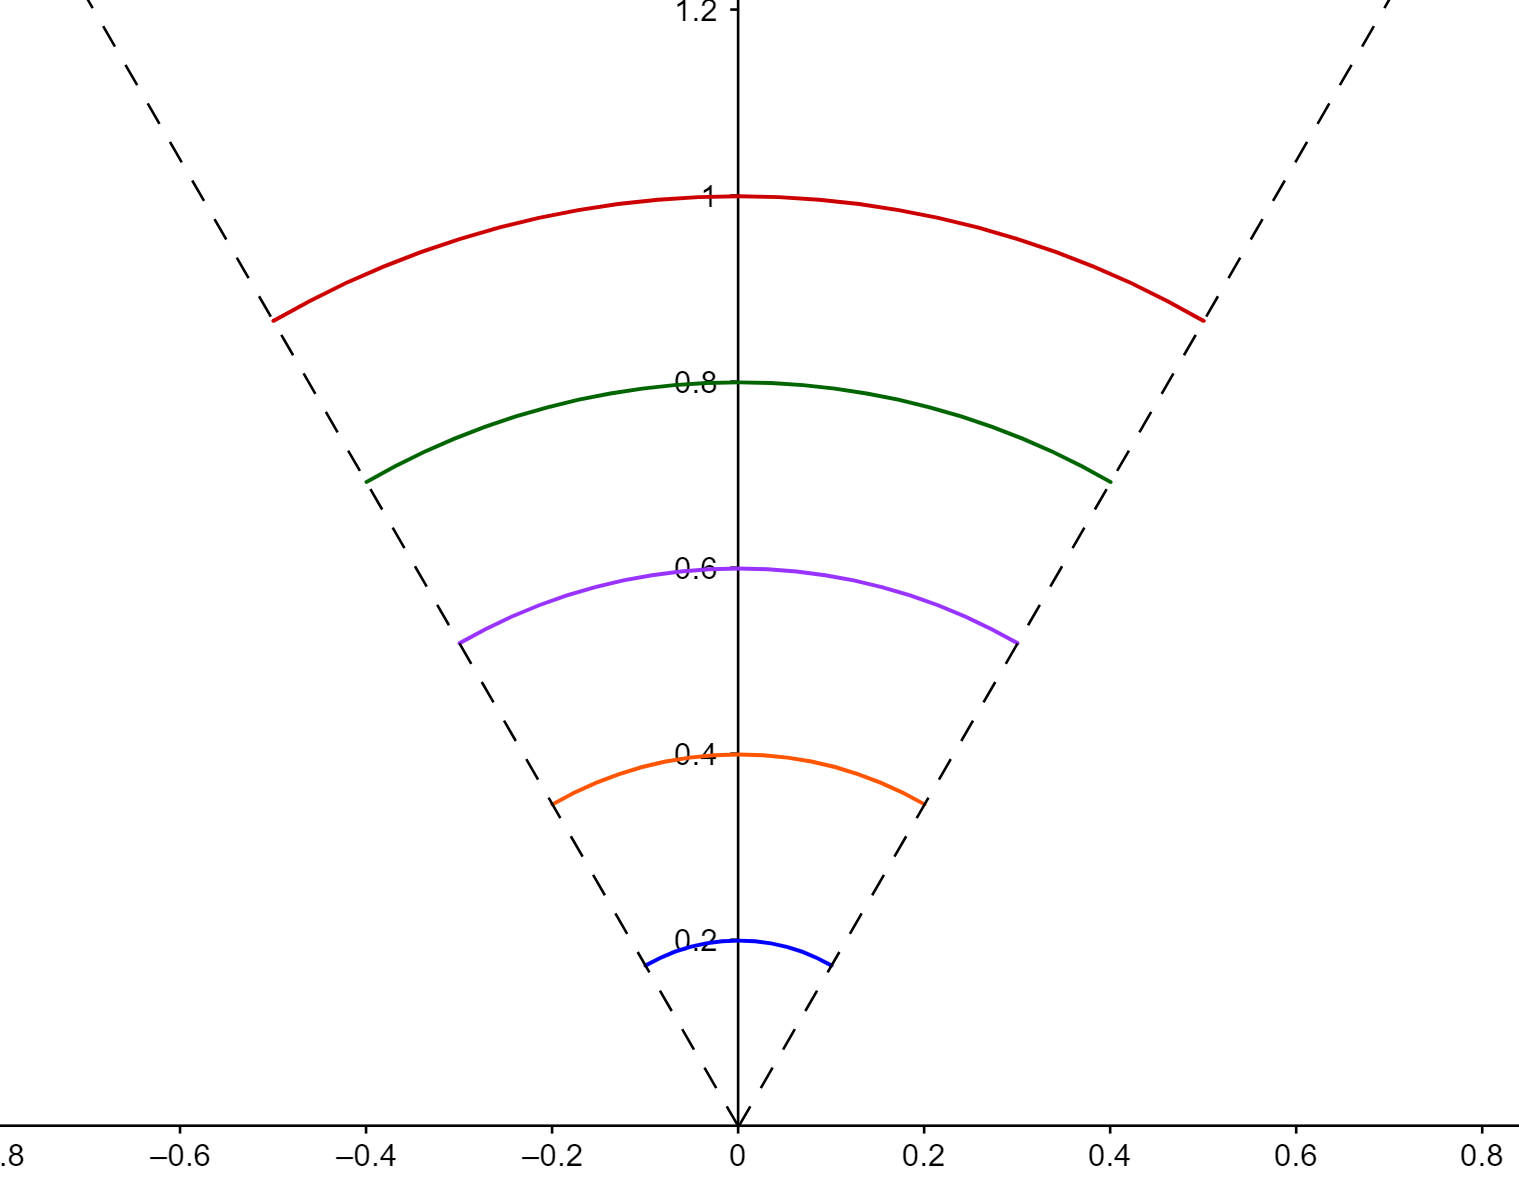
\includegraphics[width=0.4\linewidth]{images/Ex 2.1.4.3.png}
            % \caption{}
            % \label{fig:enter-label}
        \end{figure}


    \item Với mỗi số thực dương $b$, xét đường tham số $\gamma_b:[0,1]\to \hh$ cho bởi $\gamma_b(t) = t+ib$. Khi đó 
        \begin{itemize}
            \item Độ dài Euclid của $\gamma_b$ là
            \[l(\gamma_b) = \int_0^1{|\gamma'(t)|dt} = \int_0^1|1|dt = 1.\]
            không đổi với mọi $b>0$.
            \item Độ dài hyperbolic của $\gamma_b$ là
            \[h(\gamma_b) = \int_0^1|\gamma'(t)|_{hyp}dt = \int_0^1\dfrac{|\gamma'(t)|}{\im(\gamma(t))}dt = \int_0^1{\dfrac{1}{b}}dt = \dfrac{1}{b}.\]
            biến thiên, phụ thuộc vào giá trị của $b>0$. Khi $b \to \infty$ thì $h(\gamma_b) \to 0$. Ngược lại khi $b \to 0$ thì $h(\gamma_b) \to \infty$.
            \begin{figure}[htp!]
                \centering
                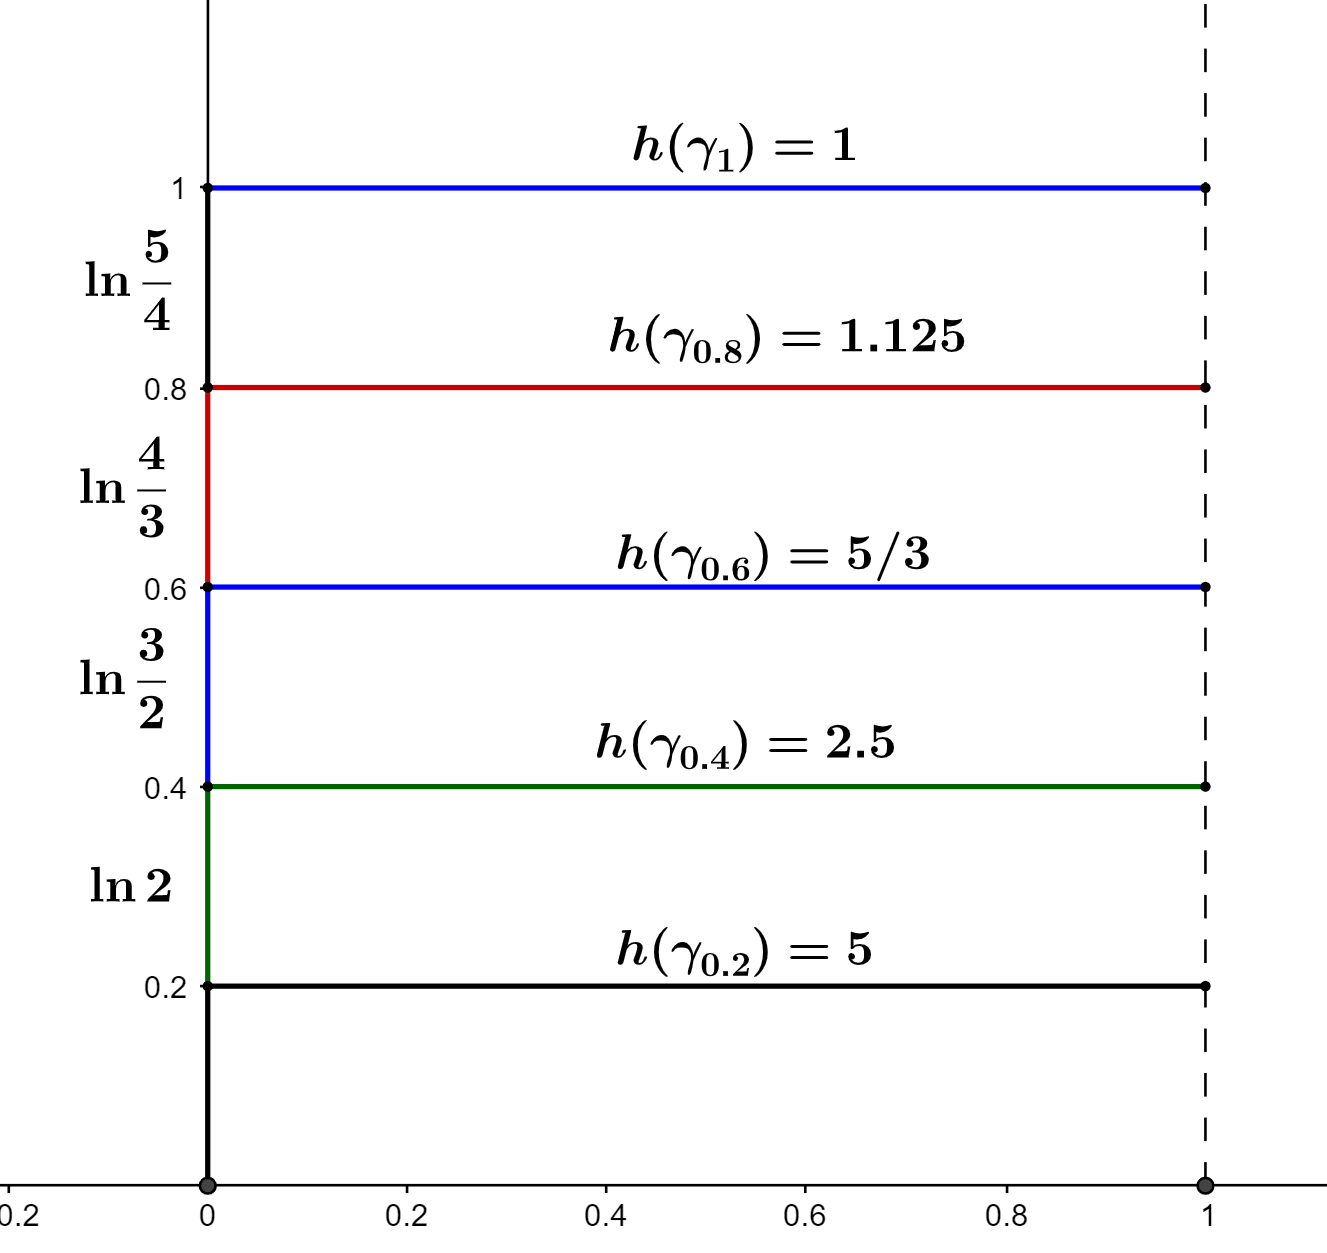
\includegraphics[width=0.5\linewidth]{images/it.png}
                % \caption{}
                % \label{fig:enter-label}
            \end{figure}
        \end{itemize}
    
        
\end{enumerate}
\end{exam*}

\begin{exam*}
    % \begin{enumerate}
        Cho $a<b$ là hai số thực dương. Khi đó độ dài hyperbolic của đường tham số $\gamma:[a,b]\to \hh$ cho bởi $\gamma(t) = it$ là
    \[h(\gamma) = \int_a^b|\gamma'(t)|_{hyp}dt = \int_a^b\dfrac{|\gamma'(t)|}{\im(\gamma(t))}dt = \int_a^b\dfrac{1}{t}dt = \ln{\dfrac{b}{a}}.\]
    %     \item Xét đường tham số $\alpha: [a,b] \to \hh,~t \mapsto ie^t$. Khi đó độ dài hyperbolic của $\gamma$ là
    %         \[h(\alpha) = \int_a^b|\alpha'(t)|_{hyp}dt = \int_a^b\dfrac{|\alpha'(t)|}{\im(\alpha(t))}dt = \int_a^b{\dfrac{e^t}{e^t}}dt = b-a.\]
            
    % \end{enumerate}
\end{exam*}
\begin{defn}
    Cho $z,w\in \hh$. \textbf{Khoảng cách hyperbolic} từ $z$ đến $w$ là 
    \[\rho(z,w) = \inf_{\gamma \in \Gamma[z,w]}{h(\gamma)}\]
    trong đó tập $\Gamma[z,w]$ là tập hợp các đường tham số trơn từng khúc từ $z$ đến $w$.
\end{defn}
Bên dưới, ta sẽ đưa ra công thức tường minh để tính khoảng cách hyperbolic giữa hai điểm bất kỳ trong $\hh$. Mệnh đề sau là vài tính chất đơn giản của hàm khoảng cách hyperbolic. Sau này, ta sẽ chỉ ra rằng hàm khoảng cách hyperbolic là một metric trên $\hh$, hơn nữa, topo sinh ra từ metric này chính là topo thông thường của $\hh$. 

\begin{prop}\label{prop 2.1.7}
    Cho $z,z_1,z_2,z_3 \in \hh$ là các điểm bất kỳ. Khi đó
    \begin{enumerate}
        \item $\rho(z,z) = 0,$
        \item $\rho(z_1,z_2) \geq 0,$
        \item $\rho(z_1,z_2) = \rho(z_2,z_1),$
        \item $\rho(z_1,z_2)+\rho(z_2,z_3) \geq \rho(z_1,z_3)$.
    \end{enumerate}
\end{prop}
\begin{proof}
    Đầu tiên ta chỉ ra $\rho$ là đối xứng, tức $\rho(z_1,z_2) = \rho(z_2,z_1)$ với mọi $z_1,z_2 \in \hh$. Thật vậy, 

        Lấy bất kỳ $\gamma:[a,b]\to \hh$ trong $\Gamma[z_1,z_2]$, cho hợp thành với song ánh khả vi sau 
    \[\tau: [a,b]\to [a,b],~t \mapsto (a+b-t).\]
    Khi đó $\sigma = \gamma\circ \tau:[a,b]\to \hh$ cũng là một hàm trơn từng khúc thoả mãn
    \[\sigma(a) = \gamma\circ \tau(a) = \gamma(b)=z_2,~\sigma(b) = \gamma\circ \tau(b) = \gamma(a)=z_1.\] 
    Chứng tỏ $\sigma \in \Gamma[z_2,z_1]$ và độ dài hyperbolic của $\sigma$ là
    \begin{align*}
        h(\sigma) = \int_{a}^{b}{\dfrac{\left|\sigma'(t)\right|}{\im(\sigma(t))}}dt = \int_{a}^{b}{\dfrac{\left|(\gamma\circ\tau)'(t)\right|}{\im((\gamma\circ\tau)(t))}}dt=\int_{a}^{b}{\dfrac{\left|\gamma'(\tau(t))\tau'(t)\right|}{\im(\gamma(\tau(t)))}}dt.
    \end{align*}
    Đặt $s = \tau(t) = a+b-t$ thì $ds = -dt$. Đổi cận $t=a$ thì $s = b$, $t=b$ thì $s=a$, kết hợp $\tau'(t) = -1$ ta được
    \begin{align*}
        h(\sigma) = -\int_{b}^{a}{\dfrac{\left|\gamma'(s)\right|}{\im(\gamma(s))}}ds = \int_{a}^{b}{\dfrac{\left|\gamma'(s)\right|}{\im(\gamma(s))}}ds = h(\gamma).
    \end{align*}
    Điều này chứng tỏ mỗi $\gamma \in \Gamma[z_1,z_2]$ sẽ tương ứng với $1-1$ với một $\sigma \in \Gamma[z_2,z_1]$, hơn nữa độ dài hyperbolic của hai đường này bằng nhau. 
    Dẫn đến 
    \[\left\{h(\gamma)~|~\gamma \in \Gamma[z_1,z_2]\} = \{h(\sigma)~|~\sigma \in \Gamma[z_2,z_1]\right\}.\]
    Lấy $\inf$ hai vế ta được 
    \[\rho(z_1,z_2) = \inf\{h(\gamma)~|~\gamma \in \Gamma[z_2,z_1]\} = \inf\{h(\sigma)~|~\sigma \in \Gamma[z_2,z_1]\} = \rho(z_2,z_1).\] 

    Tiếp theo ta chỉ ra $\rho$ thoả mãn bất đẳng thức tam giác.

    Thật vậy, giả sử $\gamma_{z_1,z_2}:[a,b]\to \hh$ và $\gamma_{z_2,z_3}:[b,c]\to \hh$ lần lượt thuộc $\Gamma[z_1,z_2]$ và $\Gamma[z_2,z_3]$. Khi đó $\gamma_{z_1,z_3}: [a,c] \to \hh$ cho bởi $\gamma_{z_1,z_3}(t) = \gamma_{z_1,z_2}(t)$ nếu $t\in[a,b]$ và $\gamma_{z_1,z_3}(t) = \gamma_{z_2,z_3}(t)$ nếu $t\in[b,c]$, là đường nối $z_1 \text{ tới }z_3$. Dẫn đến
    \[\rho(z_1,z_3) = \inf_{\gamma \in \Gamma[z_1,z_3]}\{h(\gamma)\} \leq h(\gamma_{z_1,z_3}) = h(\gamma_{z_1,z_2}) + h(\gamma_{z_2,z_3}).\]
    Lấy $\inf$ hai vế theo các đường cong trơn từng khúc nối $z_1 \text{ tới }z_2$ và nối $z_2 \text{ tới }z_3$ ta được
    \[\rho(z_1,z_3) \leq  \inf h(\gamma_{z_1,z_2}) + \inf h(\gamma_{z_2,z_3}) = \rho(z_1,z_2) + \rho(z_2,z_3).\]

    Cuối cùng ta kiểm tra tính xác định dương của $\rho$.

    Lấy $\gamma_0: [a,b] \to \hh, t \mapsto z$ là một đường cong trơn trên $\hh$ qua $z$. Ta có $\gamma_0'(t) = 0$ nên $h(\gamma_0) = 0 $. Vì vậy, $\rho(z,z) = 0$.

    Nếu $z_1 \neq z_2$, ta sẽ chỉ ra $\rho(z_1,z_2) >0$ sau.
\end{proof}
\begin{prop}\label{prop 2.1.8}
    Cho $a,b$ là hai số thực dương. Khoảng cách hyperbolic giữa các điểm $ia, ib$ là 
    \[\rho(ia,ib) = \left|\ln{\dfrac{b}{a}}\right|.\]
\end{prop}
\begin{proof}
    Xét trường hợp $0<a<b$.
    
    Xét đường cong $\gamma_0:[0,1] \to \hh,~t\mapsto x(t) + iy(t) = i(a+(b-a)t$ có đồ thị chính là đoạn thẳng Euclid trên trục ảo nối $ia$ với $ib$. Khi đó độ dài hyperbolic của $\gamma_0$ là 
    \[h(\gamma_0) = \int_{0}^{1}{\dfrac{\sqrt{(x'(t))^2+(y'(t))^2}}{y(t)}}dt = \int_{0}^{1}{\dfrac{b-a}{a+(b-a)t}}dt = \ln{|a+(b-a)t|~\bigg|_{0}^{1}} = \ln \dfrac{b}{a}.\]
    Lấy bất kì đường cong trơn từng khúc $\gamma: [0,1] \to \hh,~t \mapsto \gamma(t) = u(t) + i v(t)$ nối $ia$ và $ib$ (tức $\gamma(0)=u(0)+iv(0)=ia,~\gamma(1)=u(1)+iv(1)=ib$). Khi đó độ dài hyperbolic của $\gamma$ là
    \[h(\gamma) = \int_{0}^{1}{\dfrac{\sqrt{(u'(t))^2+(v'(t))^2}}{v(t)}}dt \geq \int_{0}^{1}{\dfrac{|v'(t)|}{v(t)}}dt \geq \int_{0}^{1}{\dfrac{v'(t)}{v(t)}}dt = \int_{a}^{b}{\dfrac{dv}{v}} = \ln\dfrac{b}{a } = h(\gamma_0)\cdot\]
    Chửng tỏ $\gamma_0$ chính là đường cong có độ dài hyperbolic ngắn nhất nối $ia$ và $ib$ trong $\hh$. Tức là $\rho(ia,ib) = \ln \dfrac{b}{a}\cdot$

    Tương tự cho trường hợp $a>b>0$ ta được $\rho(ia,ib) = \ln \dfrac{a}{b}\cdot$

    Tóm lại $\rho(ia,ib) = \left|\ln{\dfrac{b}{a}}\right|.$
\end{proof}
Để tính khoảng cách giữa hai điểm bất kỳ trong $\hh$, và xác định các trắc địa của $\hh$, ta sẽ sử dụng các đẳng cự của $\hh$.
\begin{defn}
    Một vi phôi $T:\hh \to \hh$ được gọi là một \textbf{đẳng cự} nếu với mọi $z\in \hh$ và mọi vector tiếp xúc $u,v \in T_z\hh$, ta có
    \[\left<DT_z(u),DT_z(v)\right>_{hyp} = \left<u,v\right>_{hyp}.\]
\end{defn}
\begin{prop}\label{prop 2.1.10}
    Cho $T$ là một phép đẳng cự của $\hh$.
    \begin{enumerate}
        \item Cho $\gamma$ là một đường tham số trơn từng khúc trong $\hh$. Khi đó $h(T(\gamma)) = h(\gamma)$.
        \item Cho $z,w$ là hai điểm của $\hh$. Khi đó $\rho(z,w) = \rho(T(z),T(w))$.
    \end{enumerate}
\end{prop}
\begin{proof}
    \begin{enumerate}
        \item Giả sử $\gamma: [a,b] \to \hh$ là một đường cong trơn từng khúc trong $\hh$. Khi đó
        \begin{align*}
            h(T(\gamma)) &= \int_a^b|(T\circ\gamma)'(t)|_{hyp}dt \\
            &= \int_a^b{\sqrt{\left<DT_{\gamma(t)}(\gamma'(t)),DT_{\gamma(t)}(\gamma'(t))\right>_{hyp}}}dt\\
            &= \int_a^b\sqrt{\left<\gamma'(t),\gamma'(t)\right>_{hyp}}dt\\
            &= \int_a^b|\gamma'(t)|_{hyp}dt\\
            &= h(\gamma).
        \end{align*}

        \item Với mọi $z,w \in \hh$, ta có
        \[\rho(z,w) = \inf_{\gamma\in \Gamma[z_1,z_2]}{h(\gamma)} = \inf_{\gamma\in \Gamma[z_1,z_2]}{h(T(\gamma))} = \inf_{\alpha  \in \Gamma[T(z),T(w)]}{h(\alpha)} = \rho(T(z),T(w))\]
    \end{enumerate}
\end{proof}
Tập hợp các phép đẳng cự của mặt phẳng hyperbolic lập thành một nhóm đối với phép toán hợp thành. Ta ký hiệu nhóm này là $\Isom(\hh)$ và gọi là nhóm các phép đẳng cự trên $\hh$.
\begin{prop}\label{prop 2.1.11}
    Cho $A = \matt \in \SL(2,\R)$. Xét các phép biến đổi xạ ảnh $T_A:P^1(\C) \to P^1(\C)$.
    \begin{enumerate}
        \item Với mọi $z\in \hh, T_A(z) \in \hh$. Hơn nữa
        \[T_A(z) = \dfrac{az+b}{cz+d}.\]
        \item Ánh xạ hạn chế $T_A: \hh \to \hh$ là một vi phôi.
    \end{enumerate}
\end{prop}
\begin{proof}
    \begin{enumerate}
        \item Với mọi $z\in \hh$, ta có 
            \begin{align*}
            \im(T_A(z)) &= \dfrac{1}{2i}\left(T_A(z) - \overline{T_A(z)}\right)\\
            &= \dfrac{1}{2i}\left(\dfrac{az+b}{cz+d} - \dfrac{a\overline{z}+b}{c\overline{z}+d}\right) \quad (\text{do } a,b,c,d \in \R)\\
            &= \dfrac{1}{2i}\left(\dfrac{(ad-bc)(z-\overline{z})}{|cz+d|^2}\right)\\
            &= \dfrac{\im(z)}{|cz+d|^2} > 0\quad(\text{do } z \in \hh \text{ nên } \im(z) >0).
            \end{align*}
            Chứng tỏ $T_A(z) \in \hh$ với mọi $z\in \hh$.

            \item Ta có $T_A$ là một song ánh khả vi liên tục và nghịch ảnh của nó $T_A^{-1}(z) = \dfrac{dz-b}{-cz+a}$ cũng thuộc $\PSL(2,\R)$ và cũng khả vi liên tục. Do đó $T_A$ là một vi phôi trên $\hh$.
            % \[T_A'(z) = \dfrac{ad-bc}{(cz+d)^2} = \dfrac{1}{(cz+d)^2}.\]
    \end{enumerate}
\end{proof}

Ta nói ánh xạ hạn chế $T_A: \hh \to \hh$ là phép biến đổi của mặt phẳng hyperbolic sinh bởi ma trận $A$.
\begin{prop}\label{prop 2.2.12}
    Cho $A\in \SL(2,\R)$. Khi đó, phép biến đổi $T_A:\hh \to \hh$ của mặt phẳng hyperbolic sinh ra bởi ma trận $A$ là một đẳng cự.
\end{prop}
\begin{proof}
    Giả sử $A = \matt$.  Khi đó phép biến đổi của mặt phẳng hyperbolic sinh bởi $A$ là $T_A(z) = \dfrac{az+b}{cz+d}$. Với mọi $z\in \hh$ và với mọi $u,v \in T_z\hh$ ta có
    \begin{align*}
        \left<(DT_A)_z(u),(DT_A)_z(v)\right>_{hyp} 
        &= \left<\dfrac{1}{(cz+d)^2}(u),\dfrac{1}{(cz+d)^2}(v)\right>_{hyp} \\
        & = \dfrac{\dfrac{1}{(cz+d)^2}(u) \cdot \dfrac{1}{(cz+d)^2}(v)}{\im^2(T_A(z))}\\
        &= \dfrac{\left|\dfrac{1}{(cz+d)^2}\right|u\cdot v}{\left(\dfrac{\im(z)}{|cz+d|^2}\right)}\\
        &= \dfrac{u\cdot v}{\im^2(z)}\\
        &= \left<u,v\right>_{hyp}.
    \end{align*}
    Chứng tỏ $T_A$ là một đẳng cự trên $\hh$.
\end{proof}

Ta nhận được đồng cấu nhóm 
\begin{equation}\label{equ 2.1.1}
\SL(2,\R) \to \Isom(\hh),\quad A \mapsto T_A.
\end{equation}
\begin{prop}\label{prop 2.1.13}
    Hạt nhân của đồng cấu nhóm \ref{equ 2.1.1} là nhóm con của $\SL(2,\R)$ bao gồm hai ma trận $\begin{bmatrix}
        1 & 0\\
        0 & 1
    \end{bmatrix}, \begin{bmatrix}
        -1 & 0\\
        0 & -1
    \end{bmatrix}$. Do đó đồng cấu nhóm \ref{equ 2.1.1} cảm sinh đơn cấu $\PSL(2,\R) \to \Isom(\hh)$. 
\end{prop}
\begin{proof}
    Đồng cấu nhóm $\phi: \SL(2,\R) \to \Isom(\hh),A \mapsto T_A$ có hạt nhân \[\ker(\phi) = \{A \in \SL(2,\R): T_A = \Id\}\]

    Để $A  = \matt \in \ker(\phi)$ thì $z = T_A(z) = \dfrac{az+b}{cz+d}$  với mọi $z\in \hh$.
    Đồng nghĩa với việc phương trình $cz^2+(d-a)z+b = 0$ có vô số nghiệm. Điều này xảy ra khi và chỉ khi $c=d-a=b=0$. Kết hợp $ad-bc=1$ ta thu được $b=c=0, a=d=\pm 1$. Do đó $\ker(\phi)= \{\pm I_2\}$, với $I_2$ là ma trận đơn vị cỡ 2.

    Khi đó $\PSL(2,\R) = \SL(2,\R)/\ker(\phi) \cong \im(\phi) \leq \Isom(\hh)$ cảm sinh một đơn cấu $\PSL(2,\R) \to \Isom(\hh)$.
\end{proof}
Sử dụng đơn cấu $\PSL(2,\R) \to \Isom(\hh)$ trong mệnh đề trên, ta thường coi $\PSL(2,\R)$ là một nhóm con của $\Isom(\hh)$.
% \begin{exam*}
%     Tính khoảng cách hyperbolic giữa hai điểm $z=1+i$ và $w=-3+4i$ trong $\hh$. Xác định các đường tham số $\gamma$ nối $z$ đến $w$ sao cho $h(\gamma) =\rho(z,w)$.

%     Dựa vào mệnh đề \ref{prop 2.1.8} và mệnh đề \ref{prop 2.1.10}, ta sẽ tìm một đẳng cự $T(z) = \dfrac{az+b}{cz+d}$ gửi hai điểm $1+i$ và $-3+4i$ thành hai điểm có phần ảo dương trên trục ảo.

%     Ta tìm $a,b,c,d \in \R$ thoả mãn $ad-bc = 1$ và $T(1+i) = i$ và $\re(T(w)) = 0$. 
%     \begin{itemize}
%         \item  $T(i+1) = i \Leftrightarrow \dfrac{a(1+i)+b}{c(1+i)+d}=i \Leftrightarrow (a+b)+ia = -c +(c+d)i \Leftrightarrow a+b = -c,~a = c+d$.

%         \item $\re(T(w)) = 0 \Leftrightarrow \dfrac{1}{2}\left(\dfrac{aw+b}{cw+d}+\dfrac{a\overline{w}+b}{c\overline{w}+d}\right) = 0 \Leftrightarrow ac|w|^2+(ad+bc)\re(w)+bd = 0\Leftrightarrow 25ac-3(ad+bc) +bd = 0$.
%         \item Suy ra $25ac -3a(a-c)-3c(-c-a) +(-c-a)(a-c) = 0 \Leftrightarrow 4c^2+31ca-4a^2 = 0 \Leftrightarrow c = \dfrac{-31\pm 5\sqrt{41}}{8}a$. Ta chọn $c = \dfrac{-31+ 5\sqrt{41}}{8}a$

%         Kết hợp $1 = ad-bc = a(a-c)-(-c-a)c = a^2+c^2$, ta được $a= \dfrac{8}{\sqrt{2050-310\sqrt{41}}}$. 
        
%         Dẫn đến $c = \dfrac{-31+5\sqrt{41}}{\sqrt{2050-310\sqrt{41}}}$. Suy ra $b = \dfrac{-23-5\sqrt{41}}{\sqrt{2050-310\sqrt{41}}},~d = \dfrac{39-5\sqrt{41}}{\sqrt{2050-310\sqrt{41}}}.$

%         Do đó $T(w) = i\im(T(w)) = i \dfrac{1}{|cw+d|^2} = i\dfrac{2050-310\sqrt{41}}{38792-6040\sqrt{41}}.$

%         Khi đó $\rho(z,w) = \rho(T(z),T(w)) = \rho\left(i,i\dfrac{2050-310\sqrt{41}}{38792-6040\sqrt{41}}\right) = \ln{\dfrac{38792-6040\sqrt{41}}{2050-310\sqrt{41}}}.$

%         Do đó ta chọn được $\gamma: [1, \im(T(w))] \to \hh, ~t \to T^{-1}(it)$ là đường cong trơn qua $z,w$ thoả mãn $h(\gamma) = \rho(z,w)$.
%     \end{itemize}
    
% \end{exam*}
\begin{exam*}
    Tính khoảng cách hyperbolic giữa hai điểm $z=1+i$ và $w=-2+2i$ trong $\hh$. Xác định các đường tham số $\gamma$ nối $z$ đến $w$ sao cho $h(\gamma) =\rho(z,w)$.

    Dựa vào mệnh đề \ref{prop 2.1.8} và mệnh đề \ref{prop 2.1.10}, ta sẽ tìm một đẳng cự $T(z) = \dfrac{az+b}{cz+d}$ gửi hai điểm $1+i$ và $-2+2i$ thành hai điểm có phần ảo dương trên trục ảo.

    Ta tìm $a,b,c,d \in \R$ thoả mãn $ad-bc = 1$ và $T(1+i) = i$ và $\re(T(w)) = 0$. 
    \begin{itemize}
        \item  $T(i+1) = i \Leftrightarrow \dfrac{a(1+i)+b}{c(1+i)+d}=i \Leftrightarrow (a+b)+ia = -c +(c+d)i \Leftrightarrow b = -c-a,~d = a -c$.

        \item $\re(T(w)) = 0 \Leftrightarrow \dfrac{1}{2}\left(\dfrac{aw+b}{cw+d}+\dfrac{a\overline{w}+b}{c\overline{w}+d}\right) = 0 \Leftrightarrow ac|w|^2+(ad+bc)\re(w)+bd = 0$.
        \item Suy ra $8ac -2a(a-c)-2c(-c-a) +(-c-a)(a-c) = 0 \Leftrightarrow c^2+4ca-a^2 = 0 \Leftrightarrow c = (-2\pm \sqrt{5})a$. Ta chọn $c = (-2+ \sqrt{5})a$. 

        Kết hợp $1 = ad-bc = a(a-c)-(-c-a)c = a^2+c^2$, ta được $a^2=\dfrac{1}{10-4\sqrt{5}}$. 
        
        Chọn $a = \dfrac{1}{\sqrt{10-4\sqrt{5}}}$. Suy ra $c = \dfrac{-2+\sqrt{5}}{\sqrt{10-4\sqrt{5}}}, b = \dfrac{1-\sqrt{5}}{\sqrt{10-4\sqrt{5}}},~d = \dfrac{3-\sqrt{5}}{\sqrt{10-4\sqrt{5}}}.$

        Do đó $T(w) = i\im(T(w)) = i \dfrac{\im(w)}{|cw+d|^2} = i\dfrac{7+3\sqrt{5}}{2}.$

        Khi đó $\rho(z,w) = \rho(T(z),T(w)) = \rho\left(i,i\dfrac{7+3\sqrt{5}}{2}\right) = \ln{\dfrac{7+3\sqrt{5}}{2}}.$

        Do đó ta chọn được $\gamma: [1, \im(T(w))] \to \hh, ~t \to T^{-1}(it)$ là đường cong trơn qua $z,w$ thoả mãn $h(\gamma) = \rho(z,w)$.
    \end{itemize}
    
\end{exam*}

\section{Trắc địa}
\begin{defn}
    Một đường tham số tốc độ đơn vị $\gamma: I\to \hh$ được gọi là một \textbf{trắc địa} nếu với mọi $t,s \in I$ với $t\leq s$, ta có
    \[\rho(\gamma(s),\gamma(t)) = h(\gamma|_{[t,s]}).\]
\end{defn}
\begin{remark*}
    Đường tham số $\gamma: I\to \hh$ được gọi là có tốc độ đơn vị
    nếu với mọi $t\in I$ thì \[1 = |\gamma'(t)|_{hyp} = \dfrac{|\gamma'(t)|}{\im(\gamma(t))} \Leftrightarrow |\gamma'(t)| = \im(\gamma(t)).\]
\end{remark*}
Trong định nghĩa trên, nhận xét rằng $\gamma|_{[t,s]}$ là đường cong từ $\gamma(t)$ đến $\gamma(s)$. Do đó ta luôn có 
\[\rho(\gamma(t),\gamma(s)) \leq h(\gamma|_{[t,s]}).\]
Mặt khác, vì ta giả sử $\gamma$ là một đường tham số tốc độ đơn vị nên $h(\gamma_{[t,s]}) = s-t$.

Ta thấy rằng các đường trắc địa trong mặt phẳng hyperbolic $\hh$ là sự tương tự của các đoạn thẳng trong mặt phẳng Euclid $\R^2$.

Ta thường đồng nhất trắc địa $\gamma$ trong $\hh$ với vết của nó, và do đó, ta cũng gọi vết của trắc địa $\gamma$ là một trắc địa trong $\hh$.

\begin{exam*}
    Đường tham số $\gamma:\R \to \hh$ cho bởi $\gamma(t) = ie^{t}$ là một trắc địa của $\hh$. Vết của $\gamma$ là $\{ir~|~r\in \R_{>0}\}$.

    Thật vậy, ta có với mọi $t\in \R$ thì $|\gamma'(t)|_{hyp} = \dfrac{|\gamma'(t)|}{\im(\gamma(t))} = \dfrac{|ie^t|}{\im(ie^t)} = \dfrac{e^t}{e^t} = 1$.
    
    Chứng tỏ $\gamma$ là một đường tham số tốc độ đơn vị. 
    Nên với mọi $t\leq s$ thì \[h(\gamma|_{[t,s]}) = \int_t^s|\gamma'(t)|_{hyp}dt = s-t.\]

    Mặt khác, theo mệnh đề \ref{prop 2.1.8} thì $ \rho(\gamma(t),\gamma(s)) = \gamma(ie^t,ie^s) = \left|\ln{\dfrac{e^t}{e^s}}\right| = s-t$.

    Vì vậy $\rho(\gamma(t),\gamma(s)) = h(\gamma|_{[t,s]})$.
\end{exam*}
Ta muốn xác định tất cả các trắc địa của mặt phẳng hyperbolic $\hh$.
\begin{prop}\label{prop 2.2.3}
    Cho $T$ là một phép đẳng cự của $\hh$ và $\gamma$ là một trắc địa của $\hh$. Khi đó, đường tham số $T(\gamma)$ cũng là một trắc địa của $\hh$.
\end{prop}
\begin{proof}
    Giả sử $\gamma: I \to \hh$ là một trắc địa của $\hh$. Khi đó với mọi $t,s \in I, t \leq s$ thì
    \[\rho(\gamma(s),\gamma(t)) = h(\gamma_{[t,s]})\]
    
    Với $T$ là một đẳng cự trong $\hh$ thì $T\circ \gamma: I \to \hh, t \mapsto T(\gamma(t))$. Khi đó, với mọi $t,s \in I, t \leq s$, sử dụng mệnh đề \ref{prop 2.1.10} ta có
    \[\rho(T(\gamma(s)),T(\gamma(t))) = \rho(\gamma(s),\gamma(t)) = h(\gamma_{[t,s]}) = h(T(\gamma)|_{[t,s]})\]
    Chứng tỏ $T(\gamma)$ cũng là một trắc địa của $\hh$.
\end{proof}
\begin{cor}\label{cor 2.2.4}
    Với mỗi ma trận $\matt \in \SL(2,\R)$, đường cong 
    \[\left\{\dfrac{iar+b}{icr+d}: r \in \R_{>0}\right\} \subset \hh\]
    là một trắc địa của $\hh$.
\end{cor}
\begin{proof}
    Ta có $T(z) = \dfrac{az+b}{cz+d}$ là một đẳng cự trên $\hh$ và $\gamma: \R_{>0} \to \hh, t\mapsto ie^t$ là một trắc địa của $\hh$. Do đó theo mệnh đề \ref{prop 2.2.3} thì $T(\gamma)$ cũng là một trắc địa của $\hh$. Vết của $T(\gamma)$ là $\left\{\dfrac{iae^t+b}{ice^t+d}: t \in \R_{>0}\right\} = \left\{\dfrac{iar+b}{icr+d}: r \in \R_{>0}\right\}$.
\end{proof}
Ta muốn mô tả hình học cho các trắc địa của $\hh$ trong hệ quả trên. Muốn vậy, ta cần sử dụng một số kết quả cơ bản của phép biến đổi phân tuyến tính của $P^1(\C)$.
\begin{defn}
    Một \textbf{đường tròn suy rộng} trong $P^1(\C)$ là một đường tròn trong $\C$ hoặc hợp của một đường thẳng trong $\C$ với $\{\infty\}$.
\end{defn}
\begin{exam*}
    Một đường tròn suy rộng trong $P^1(\C)$ là $P^1(\R) = \R \cup \{\infty\}$.
\end{exam*}
Mệnh đề sau cho ta cách mô tả chung cho tất cả các đường tròn suy rộng.
\begin{prop}\label{prop 2.2.7}
    Đường tròn suy rộng trong $P^1(\C)$ là tập các điểm $[z:w]$ thoả mãn một phương trình có dạng
    \[(z\quad w)H\binom{\overline{z}}{\overline{w}} = 0\]
    trong đó $H \in \Mat(2,\C)$ là một ma trận Hermite, tức là $\overline{H} = H^T$.
\end{prop}
\begin{proof}
    Giả sử $C$ là một đường tròn suy rộng trong $\C$. Khi đó ta có hai trường hợp sau
    \begin{enumerate}
        \item $C$ là một đường tròn trong $\C$, giả sử tâm $\alpha \in \C$, bán kính $r>0$.

        Khi đó 
        $r^2 = |z-\alpha|^2 ~\forall z \in C$, tức là
        $r^2 = (z-\alpha)\overline{(z-\alpha)} = z\overline{z}-z\overline{\alpha} - \alpha \overline{z} + |\alpha|^2$.

        Do đó
        \[(z\quad 1)\begin{pmatrix}
            1 & -\overline{\alpha}\\
            -\alpha & |\alpha|^2-r^2
        \end{pmatrix}
        \begin{pmatrix}
            \overline{z}\\ 1
        \end{pmatrix} = 0\]
        với $\begin{pmatrix}
            1 & -\overline{\alpha}\\
            -\alpha & |\alpha|^2-r^2
        \end{pmatrix}$ là một ma trận Hermite.
        
        Vậy mọi $[z:w] \in C$ đều thoả mãn \[(z\quad w)\begin{pmatrix}
            1 & -\overline{\alpha}\\
            -\alpha & |\alpha|^2-r^2
        \end{pmatrix}\binom{\overline{z}}{\overline{w}} = 0.\]
        \item $C$ là hợp của một đường thẳng $L$ trong $\C$ với $\{\infty\}$, trong đó $L$ tạo với đường thẳng $\{z\in \C~|~\re(z) = r\}$ một góc $\theta$. Tức là $L = e^{i\theta}\{z\in \C~|~\re(z) = r\}.$

        Khi đó $z\in L \Leftrightarrow \re(e^{-i\theta}z) = r \Leftrightarrow e^{i\theta}\overline{z} + e^{-i\theta}z - 2r = 0 \Leftrightarrow (z \quad 1)\begin{pmatrix}
            0 & e^{-i\theta}\\
            e^{i\theta} & -2r
        \end{pmatrix}\begin{pmatrix}
            \overline{z} \\ 1
        \end{pmatrix} = 0$,
        
        trong đó $\begin{pmatrix}
            0 & e^{-i\theta}\\
            e^{i\theta} & -2r
        \end{pmatrix}$ là một ma trận Hermite.

        Nói riêng, $(1 \quad 0)\begin{pmatrix}
            0 & e^{-i\theta}\\
            e^{i\theta} & -2r
        \end{pmatrix}\begin{pmatrix}
            1 \\ 0
        \end{pmatrix} = 0.$

        Do đó, mọi điểm $[z:w]$ của $C = L \cup \{\infty\}$ đều thoả mãn 
        $(z\quad w)\begin{pmatrix}
            0 & e^{-i\theta}\\
            e^{i\theta} & -2r
        \end{pmatrix}\begin{pmatrix}
            \overline{z}\\ \overline{w}
        \end{pmatrix} = 0$. 
    \end{enumerate}
\end{proof}
Như vậy, các ma trận Hermite tương ứng với các đường tròn suy rộng $C$ trong $P^1(\C)$ có dạng 
\begin{enumerate}
    \item $H = \begin{pmatrix}
            1 & -\overline{\alpha}\\
            -\alpha & |\alpha|^2-r^2
        \end{pmatrix}$ nếu $C$ là đường tròn tâm $\alpha$ bán kính $r$.
    \item $H = \begin{pmatrix}
            0 & e^{-i\theta}\\
            e^{i\theta} & -2r
        \end{pmatrix}$ với $C$ là hợp của một đường thẳng trong $\C$ với $\{\infty\}$.
\end{enumerate}
Khái niệm ma trận Hermite là phiên bản phức của khái niệm ma trận đối xứng hệ số thực. Hơn nữa, một ma trận $\hh \in \Mat(2,\R)$ là một ma trận Hermite khi và chỉ khi nó là một ma trận đối xứng. 
\begin{prop}\label{prop 2.2.8}
    Cho $A \in \GL(2,\C)$. Khi đó, phép biến đổi xạ ảnh $T_A: P^1(\C)\to P^1(\C)$ biến một đường tròn suy rộng thành một đường tròn suy rộng.
\end{prop}
\begin{proof}
    Giả sử $C$ là một đường tròn suy rộng trong $P^1(\C)$. Khi đó, mọi điểm xạ ảnh $[z:w] \in C$ đều thoả mãn \[(z\quad w)H\binom{\overline{z}}{\overline{w}} = 0,\]
    trong đó $H$ là một ma trận Hermite.
    
    Đặt $[z':w'] = T_A([z:w])$, khi đó $\begin{pmatrix}
        z'\\w'
    \end{pmatrix} = A\begin{pmatrix}
        z\\w
    \end{pmatrix} \Leftrightarrow \begin{pmatrix}
        z\\w
    \end{pmatrix} = B\begin{pmatrix}
        z'\\w'
    \end{pmatrix}$, với $B = A^{-1}$.

    Khi đó
    \begin{align*}
        (z\quad w)H\begin{pmatrix}
            \overline{z}\\
            \overline{w}
        \end{pmatrix} = 0 \Leftrightarrow (z' \quad w')B^TH\overline{B}\begin{pmatrix}
            \overline{z'}\\
            \overline{w'}
        \end{pmatrix} = 0.
    \end{align*}
    Vì $(B^TH\overline{B})^T = \overline{B}^TH^TB = \overline{B^T}~\overline{H}~ \overline{\overline{B}}=\overline{B^TH\overline{B}}$, nên nó là một ma trận Hermite. 
    
    Do đó $T_A(C)$ là một đường tròn suy rộng trong $P^1(\C)$.
\end{proof}
\begin{cor}\label{cor 2.2.9}
    Với mỗi ma trận $\matt \in \SL(2,\R)$, trắc địa 
    \[\left\{\dfrac{iar+b}{icr+d}: r \in \R_{>0}\right\} \subset \hh\]
    chứa trong một đường thẳng hoặc một đường tròn của $\C$.
\end{cor}
Để xác định các trắc địa của mặt phẳng hyperbolic $\hh$, các đường tròn suy rộng mà chúng ta quan tâm đặc biệt là các đường tròn suy rộng vuông góc với $P^1(\R)$. 
\begin{figure}
    \centering
    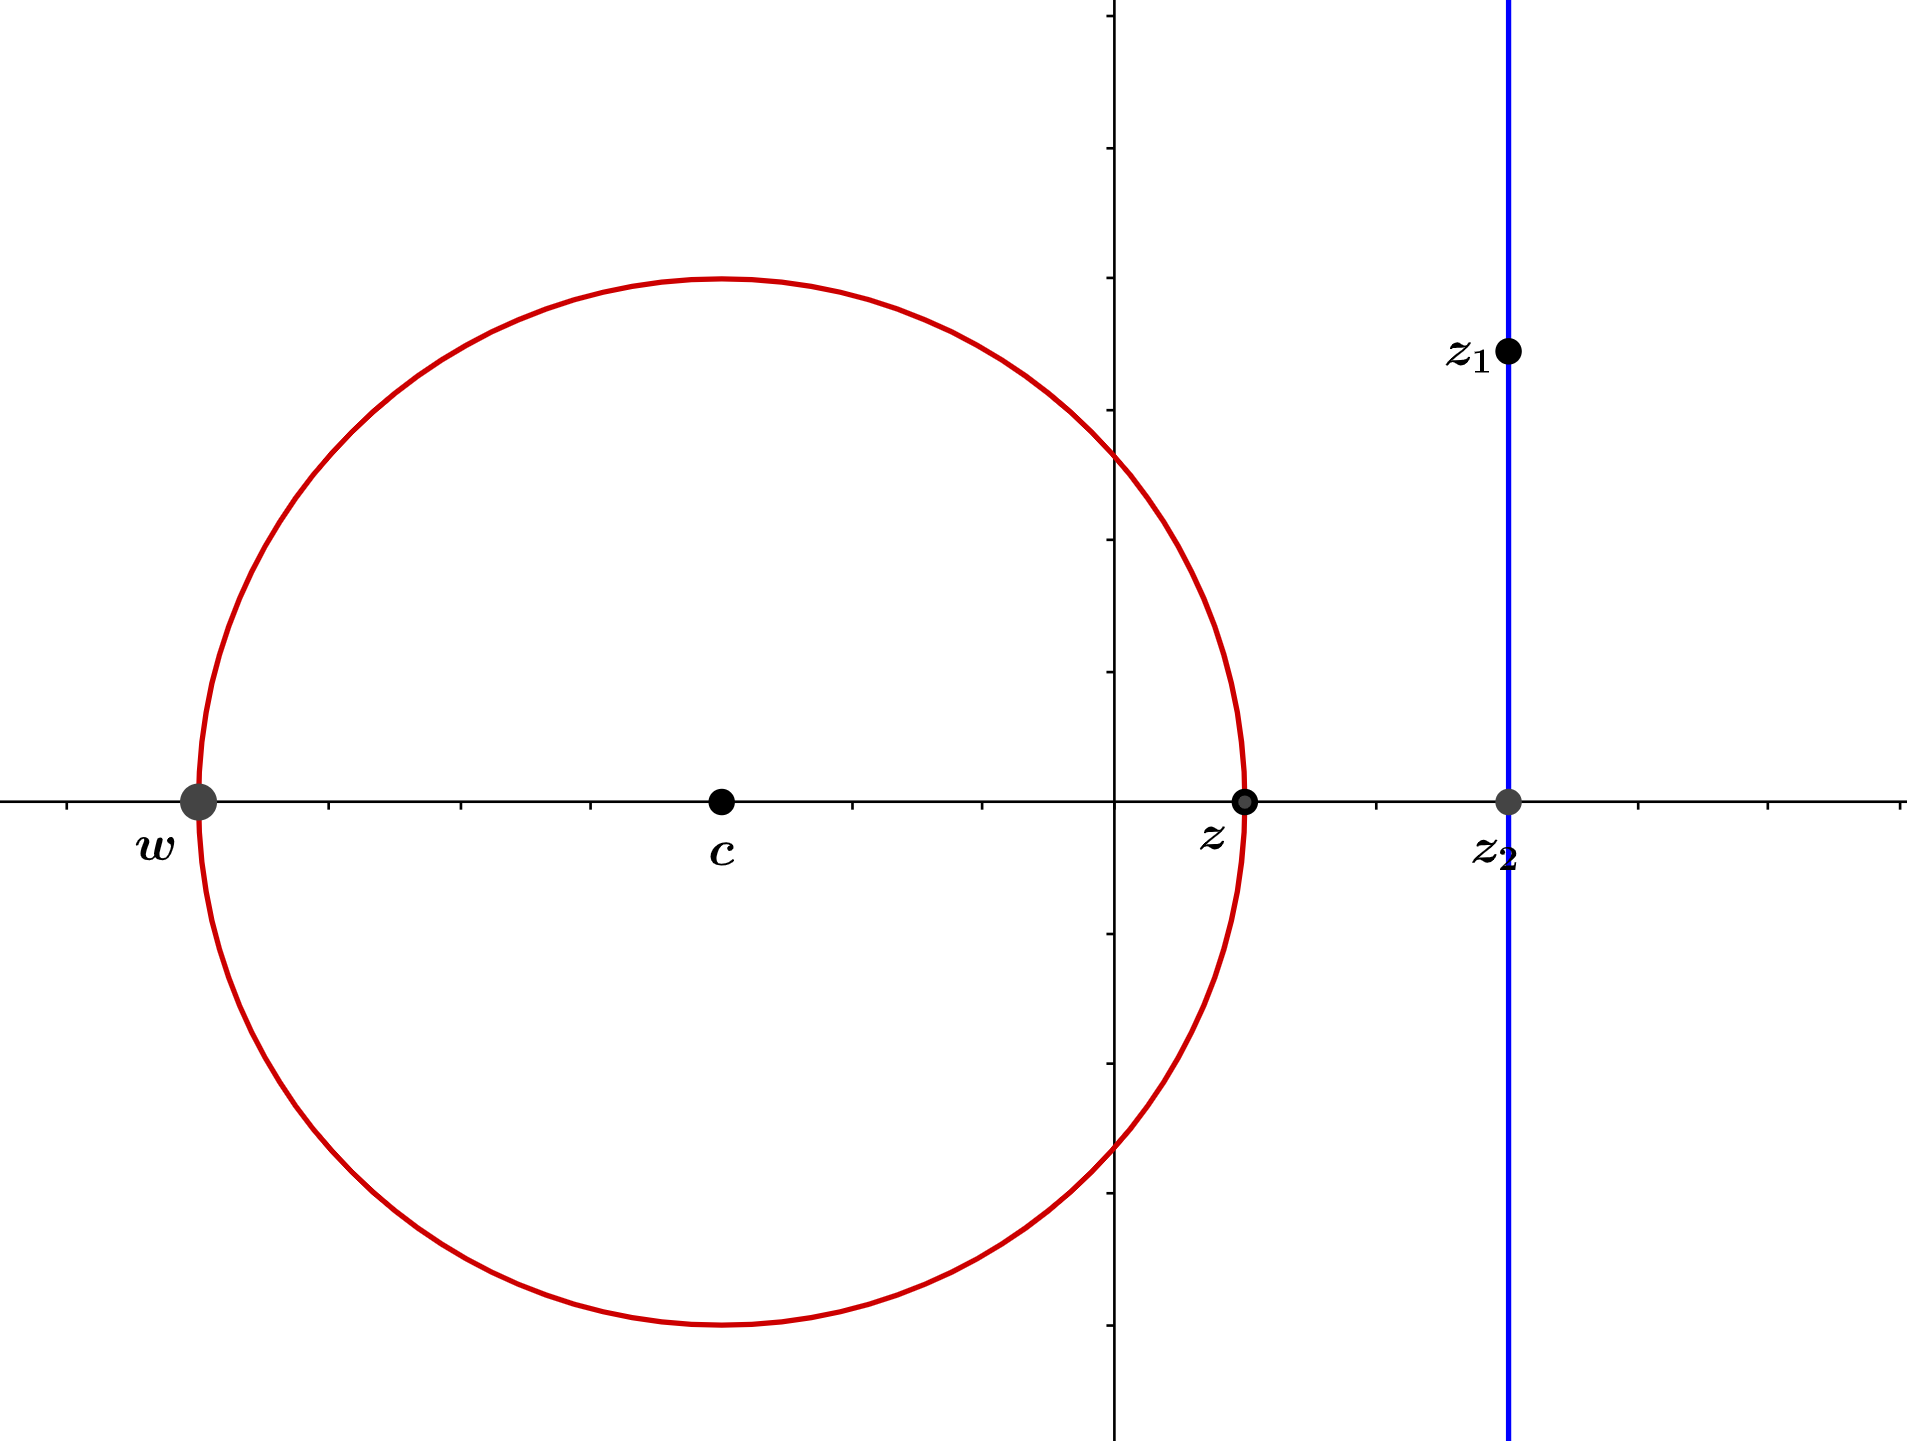
\includegraphics[width=0.55\linewidth]{images/Đường tròn trực giao R.png}
    \caption{Đường tròn suy rộng trực giao với $P^1(\R)$}
    % \label{fig:enter-label}
\end{figure}
\begin{prop}\label{prop 2.2.10}
    Các đường tròn suy rộng trong $P^1(\C)$ mà trực giao với đường tròn suy rộng $P^1(\R)$ là các đường tròn có phương trình
    \[(z\quad w)H\begin{pmatrix}
        \overline{z}\\ \overline{w}
    \end{pmatrix}\]
    trong đó $H \in \Mat(2,\C)$ là một ma trận Hermite hệ số thực.
\end{prop}
\begin{proof}
    Giả sử $C$ là một đường tròn suy rộng trong $P^1(\C)$. Khi đó, theo mệnh đề \ref{prop 2.2.7} thì ma trận Hermite tương ứng của $C$ là 
    \begin{itemize}
        \item $H = \begin{pmatrix}
            1 & -\overline{\alpha}\\
            -\alpha & |\alpha|^2-r^2
        \end{pmatrix}$ nếu $C$ là đường tròn tâm $\alpha$ bán kính $r$.

        Để $C$ trực giao với đường tròn suy rộng $P^1(\R)$ thì tâm $\alpha$ phải thuộc $\R$. Dẫn đến $H$ là một ma trận đối xứng thực. Và do đó là một ma trận Hermite hệ số thực.
        \item $H = \begin{pmatrix}
            0 & e^{-i\theta}\\
            e^{i\theta} & -2r
        \end{pmatrix}$ với $C$ là hợp của một đường thẳng $L$ trong $\C$ với $\{\infty\}$, trong đó $L$ tạo với đường thẳng $\{z\in \C~|~\re(z) = r\}$ góc $\theta$.

        Để $C$ trực giao với đường tròn suy rộng $P^1(\R)$ thì $C$ phải vuông góc với trục thực, tức là $\theta = 0$. Khi đó $H = \begin{pmatrix}
            0 & 1\\
            1 & -2r
        \end{pmatrix}$ là một ma trận đối xứng thực. Và do đó là một ma trận Hermite hệ số thực.
    \end{itemize}
\end{proof}
\begin{cor}\label{prop 2.2.11}
    Cho $A\in \SL(2,\R)$. Phép biến đổi xạ ảnh $T_A: P^1(\C) \to P^1(\C)$ biến một đường tròn suy rộng vuông góc với $P^1(\R)$ thành một đường tròn suy rộng cũng vuông góc với $P^1(\R)$.
\end{cor}
\begin{proof}
    Áp dụng mệnh đề \ref{prop 2.2.8} thì $T_A$ biến một đường tròn suy rộng $C$, có ma trận Hermite tương ứng là $H$, thành một đường tròn suy rộng $C'$, có ma trận Hermite tương ứng là $B^TH\overline{B}$, trong đó $B = A^{-1}$.

    Nếu $C$ trực giao với $P^1(\R)$ thì $H$ là một ma trận Hermite hệ số thực. Mà $B=A^{-1}$ cũng là ma trận hệ số thực nên $\overline{B} = B$. Từ đó $B^TH\overline{B}$ cũng là một ma trận Hermite hệ số thực. Tức là $C'$ cũng trực giao với $P^1(\R)$.

\end{proof}

\begin{defn}
    Một \textbf{đường hyperbolic} của $\hh$ là giao của $\hh$ với một đường tròn suy rộng vuông góc với $P^1(\R)$.
    
    Với $r,s \in P^1(\R)$ là hai điểm phân biệt, kí hiệu $h-line(r,s)$, là đường hyperbolic ứng với đường tròn suy rộng đi qua $r,s$.
\end{defn}
Nhận xét rằng đường hyperbolic $h-line(r_1,s_1)$ trùng với đường hyperbolic $h-line(r_2,s_2)$ khi và chỉ khi $\{r_1,s_1\} = \{r_2,s_2\}$.
\begin{exam*}
    Cho $r,s \in \R$ là hai số thực phân biệt.
    \begin{itemize}
        \item Đường hyperbolic $h-line(r,\infty)$ là một nửa đường thẳng.
        \item Đường hyperbolic $h-line(r,\infty)$ là một trắc địa của $\hh$.
        \item Đường hyperbolic $h-line(r,s)$ là một nửa đường tròn.
    \end{itemize}
\end{exam*}
\begin{lem}\label{lem 2.2.14}
    Tồn tại duy nhất một đường hyperbolic của $\hh$ đi qua hai điểm phân biệt bất kỳ.
\end{lem}
\begin{proof}
    Với $z_1,z_2 \in \hh, z_1 \neq z_2$, khi đó có hai trường hợp xảy ra
    \begin{enumerate}
        \item $\re(z_1) = \re(z_2) = r\in \R$.
        
        Tồn tại duy nhất đường tròn suy rộng $C = \{ z\in \C~|~\re(z) = \re(z_1)\}\cup \{\infty\}$ qua $z_1,z_2$ và vuông góc với $P^1(\R)$. Khi đó $C \cap \hh = h-line(r,\infty)$ là  đường hyperbolic duy nhất qua $z_1,z_2$.
        
        \item $\re(z_1) \neq \re(z_2)$.
        
        Khi đó không tồn tại đường thẳng vuông góc với trục thực qua $z_1,z_2$. Gọi giao điểm duy nhất của trục thực và đường trung trực của đoạn thẳng Euclid nối $z_1,z_2$ là $c$. Khi đó giao của đường tròn suy rộng tâm $c$, bán kính $|c-z_1|$ với $\hh$ chính là nửa đường hyperbolic qua $z_1,z_2$.
        \begin{figure}[htp!]
            \centering
            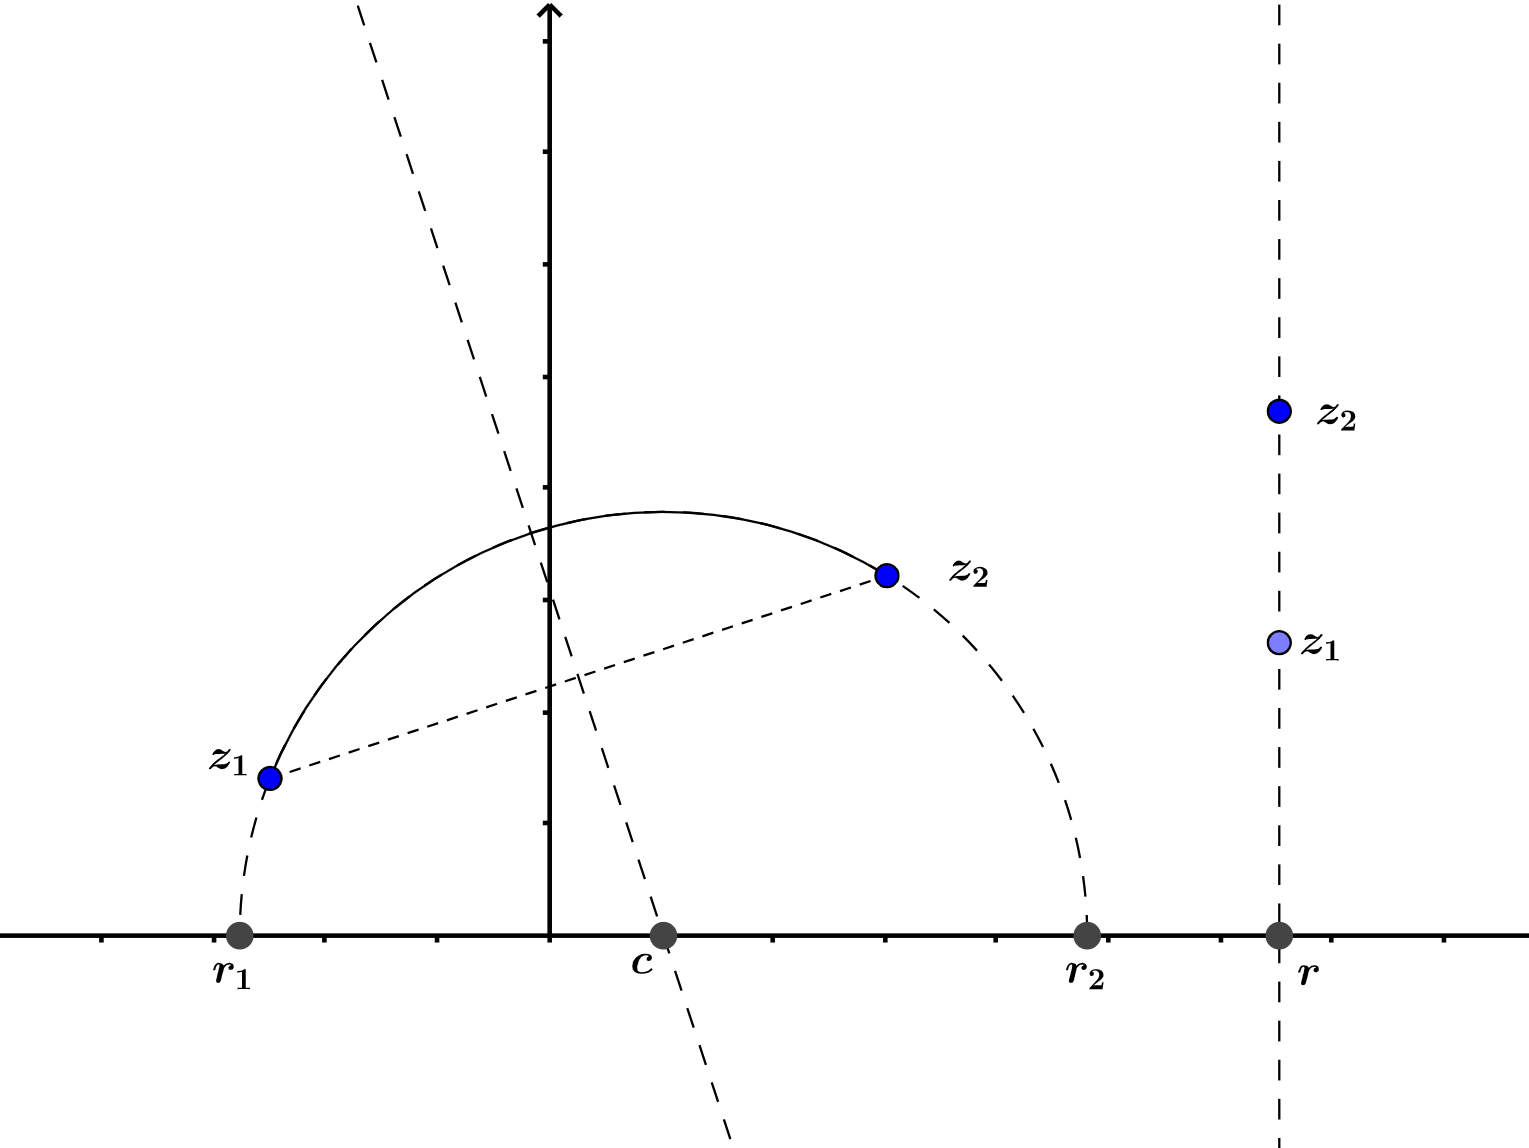
\includegraphics[width=0.5\linewidth]{images/hyperbolic-line.png}
            \caption{Đường hyperbolic trong $\hh$}
            \label{}
        \end{figure}
    \end{enumerate}
\end{proof}
\begin{prop}\label{prop 2.2.15}
    Cho $r,s \in P^1(\R)$. Tồn tại phép biến đổi $T(z) = \dfrac{az+b}{cz+d}$ của $\hh$ biến đường hyperbolic $h-line(r,s)$ thành đường hyperbolic $h-line(0,\infty)$.
\end{prop}
\begin{proof}
    Giả sử $r = [a:b], s = [c:d] \in P^1(\R)$. 
    
    Vì $r \neq s$ nên hai vector $(a,b),(c,d)$ là độc lập tuyến tính trong $\R^2$, do đó $A = \begin{pmatrix}
        a & c\\
        b & d
    \end{pmatrix}$ khả nghịch. 
    
    Đặt $k = \det(A) \neq 0$. Khi đó $\det\begin{pmatrix}
        a/k & b\\
        c/k & d
    \end{pmatrix} = 1$. Dẫn đến $ B = \begin{pmatrix}
        a/k & b\\
        c/k & d
    \end{pmatrix} \in \SL(2,\R)$. Phép biến đổi $T_B(z) = \dfrac{(a/k)z+b}{(c/k)z+d}$ của $\hh$, cảm sinh phép biến đổi xạ ảnh
    \[T_B: P^1(\C) \to P^1(\C),~ [z_1:z_2]\mapsto [(a/k)z_1+bz_2:(c/k)z_1+dz_2]\]
    Khi đó $[1:0] \mapsto [(a/k):(b/k)] = [a:b]$ và $[0:1]\mapsto [c:d]$, tức $T_B$ gửi $0\mapsto s,~\infty \mapsto r$.

    Dẫn đến phép biến đổi $T_B^{-1}$ gửi $s \mapsto 0,~r\mapsto \infty$. Nghĩa là biến $T_B^{-1}$ biến đường tròn suy rộng $C_{r,s}$ qua $r,s$ và vuông góc với $P^1(\R)$, thành đường tròn suy rộng $C_{0,\infty}$ qua $0,\infty$ và vuông góc với $P^1(\R)$. Do đó $T_B^{-1}$ biến $h-line(r,s)$ thành $h-line(0,\infty)$.
\end{proof}
\begin{cor}\label{cor 2.2.16}
    Tất cả các đường hyperbolic của $\hh$ đều là trắc địa của $\hh$.
\end{cor}
\begin{proof}
    Giả sử $r,s$ là hai điểm phân biệt trong $P^1(\R)$. Khi đó, theo mệnh đề \ref{prop 2.2.15}, tồn tại phép biến đổi $T$ của $\hh$ biến đường hyperbolic $h-line(r,s)$ thành đường hyperbolic $h-line(0,\infty)$.

    Ta đã biết $h-line(0,\infty)$ là một trắc địa trên $\hh$.
    
    Khi đó với mỗi đường cong $\gamma$ có vết trên $h-line(r,s)$ ta có
    \[\rho(\gamma(a),\gamma(b)) \leq h(\gamma|_{[a,b]}) = h(T(\gamma)|_{[a,b]}) = \rho(T(\gamma(a)),T(\gamma(b))) = \rho(\gamma(a),\gamma(b)).\]
    Dẫn đến $\rho(\gamma(a),\gamma(b)) =  h(\gamma|_{[a,b]})$, hay $\gamma$ là một trắc địa của $\hh$. 
    
    Do đó $h-line(r,s)$ cũng là một trắc địa của $\hh$.
\end{proof}
\begin{prop}\label{prop 2.2.17}
    Mọi trắc địa cực đại của $\hh$ đều là một đường hyperbolic của $\hh$.
\end{prop}
\begin{proof}
    Với mọi $p\in \hh$ và $v \in T_p\hh$. Khi đó tồn tại duy nhất một đường trắc địa cực đại $\gamma: I \to \hh$ thoả mãn $\gamma(0) = p, \gamma'(0) = v$. 
    
    Mặt khác qua $p$ có duy nhất một đường hyperbolic tiếp xúc với $v$. Thật vậy, nếu $v$ có phương vuông góc với trục thực thì tồn tại duy nhất đường hyperbolic qua $p$ và tiếp xúc với $v$ là $h-line(\re(p),\infty)$. Còn nếu $v$ có phương không vuông góc với trục thực, qua $p$ kẻ đường thẳng vuông góc với $v$, đường thẳng này cắt trục thực tại điểm duy nhất. Giả sử là $c$. Khi đó tồn tại duy nhất một đường hyperbolic qua $p$ và tiếp xúc với $v$ là nửa đường tròn có tâm $c$ và bán kính $|c-p|$.

    Mặt khác mọi đường hyperbolic đều là đường trắc địa trong $\hh$. Do đó đường hyperbolic qua $p$ và tiếp xúc với $v$ tại $p$ nói trên chính là đường trắc địa cực đại.
    \begin{figure}[htp!]
        \centering
        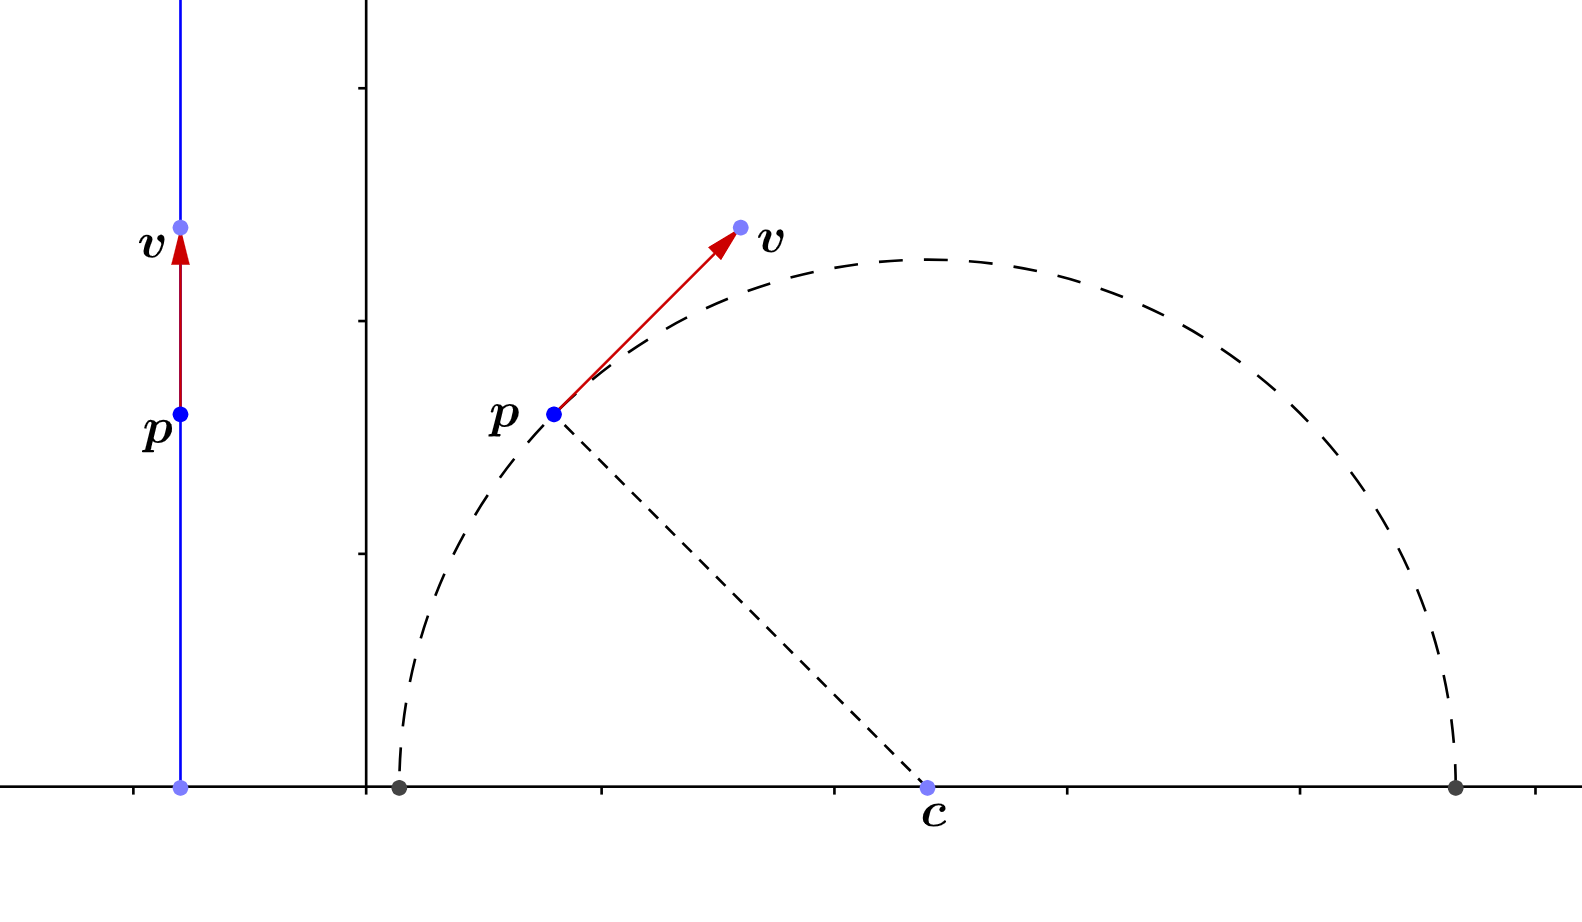
\includegraphics[width=0.5\linewidth]{images/maximum_geodesic.png}
        \caption{đường trắc địa cực đại}
        \label{fig:enter-label}
    \end{figure}
    
\end{proof}
Như vậy, ta đã xác định tất cả các trắc địa cực đại của $\hh$.
\begin{cor}\label{cor 2.2.18}
    Tồn tại duy nhất một trắc địa cực đại của $\hh$ đi qua hai điểm phân biệt bất kỳ.
\end{cor}
\begin{proof}
    Do qua hai điểm bất kì có duy nhất một đường hyperbolic và các đường hyperbolic thì là trắc địa cực đại nên tồn tại duy nhất một trắc địa cực đại của $\hh$ đi qua chúng.
\end{proof}






% \subsection{Đường hyperbolic}
% \begin{defn}[Các đường hyperbolic]

% \begin{enumerate}
%     \item Một \textit{đường thẳng hyperbolic} trong $\hh$ là tập giao của $\hh$ với đường thẳng Euclid vuông góc với trục thực. Nếu giao điểm của đường thẳng trên với trục thực là tại $r\in \R$, thì đường thẳng hyperbolic được kí hiệu bởi $\Axis(r)$. 

%     Nói riêng, $\Axis(0)$ chính là trục ảo của mặt phẳng $\hh$.
    
%     \item Một \textit{nửa đường tròn hyperbolic} trong $\hh$ là tập giao của $\hh$ với một đường tròn Euclid có tâm nằm trên trục thực và cắt trục thực tại 2 điểm phân biệt. Nếu hai giao điểm đó là $r_1,r_2$, thì nửa đường tròn hyperbolic được kí hiểu bởi $\Cir(r_1,r_2)$.
%     \end{enumerate}
% \end{defn}

% \begin{thm}\label{2.2.2}
% Mỗi cặp điểm phân biệt trong $\hh$ có duy nhất một đường hyperbolic đi qua chúng.
% \end{thm}
% \begin{proof}
%     Với $z_1,z_2 \in \hh, z_1 \neq z_2$, khi đó có hai trường hợp xảy ra
%     \begin{enumerate}
%         \item $\re(z_1) = \re(z_2)$.
        
%         Tồn tại duy nhất đường thẳng Euclid $l = \{ z\in \C~|~\im(z) = \re(z_1)\} \subset \C$ qua $z_1,z_2$ và vuông góc với trục thực. Khi đó $\Axis(\re(z_1)) = l \cap \hh $ là  đường thẳng hyperbolic duy nhất qua $z_1,z_2$.
        
%         \item $\re(z_1) \neq \re(z_2)$.
        
%         Khi đó không tồn tại đường thẳng vuông góc với trục thực qua $z_1,z_2$. Gọi giao điểm duy nhất của trục thực và đường trung trực của đoạn thẳng Euclid nối $z_1,z_2$ là $c$. Khi đó giao của đường tròn Euclid tâm $c$, bán kính $|c-z_1|$ với $\hh$ chính là nửa đường tròn hyperbolic qua $z_1,z_2$.
%         \begin{figure}[htp!]
%             \centering
%             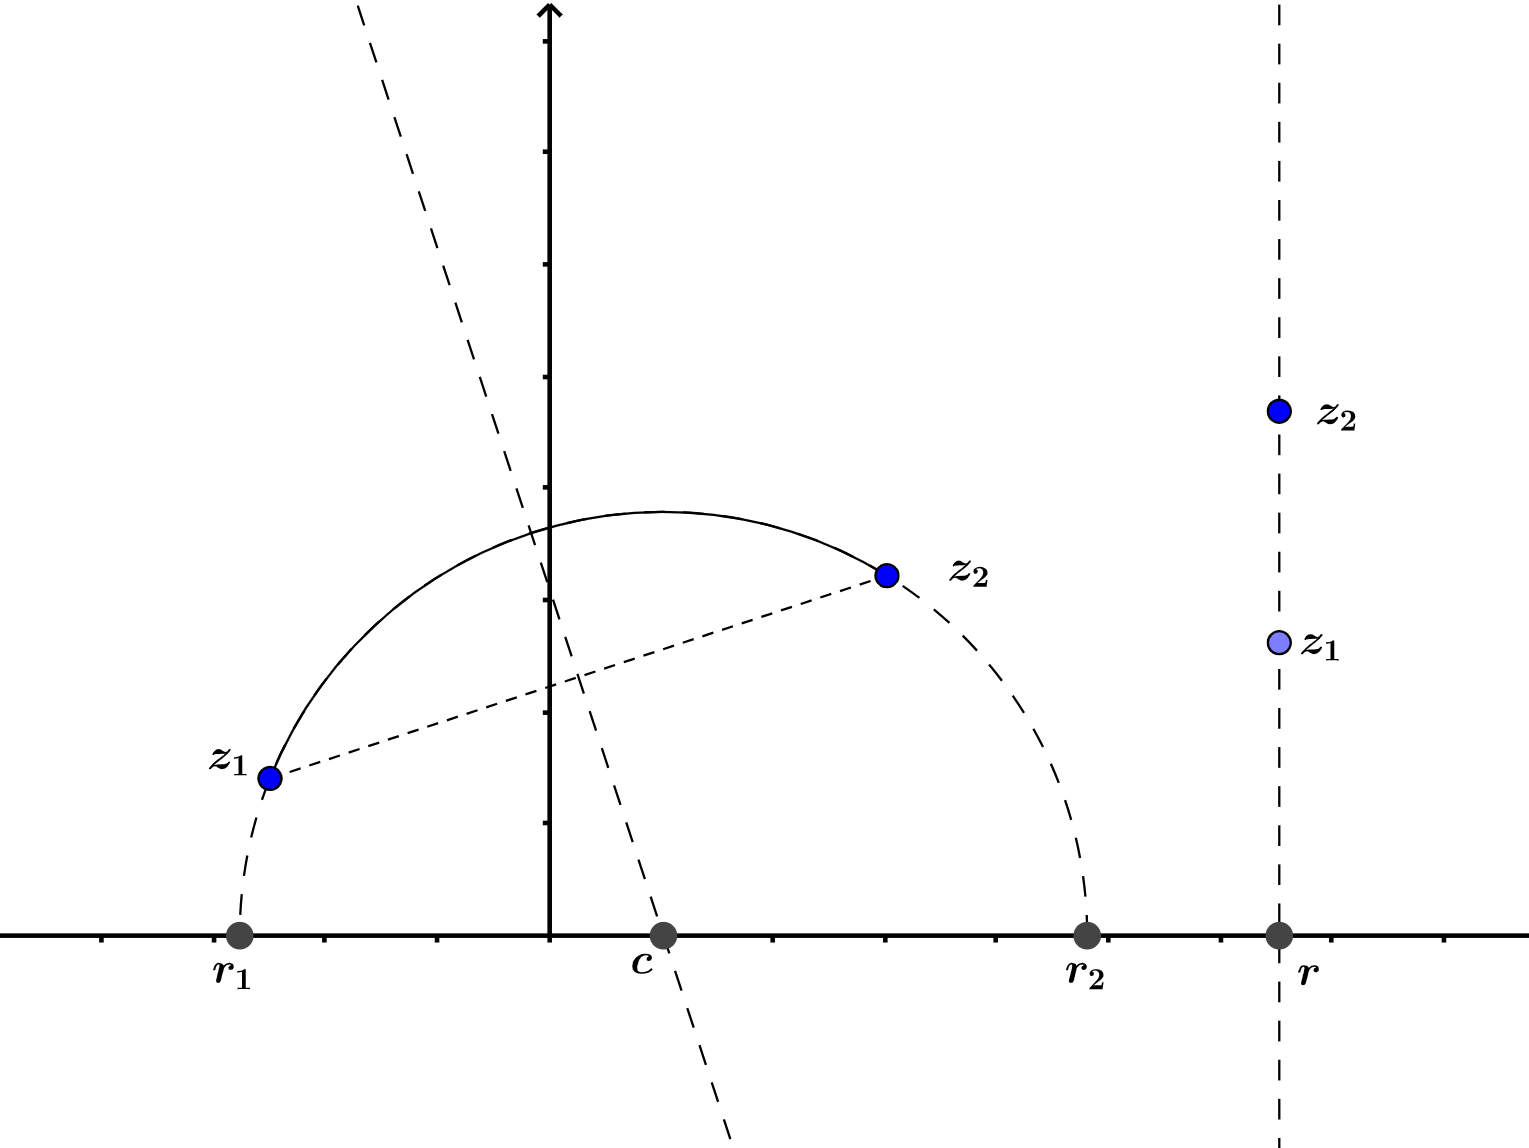
\includegraphics[width=0.6\linewidth]{images/hyperbolic-line.png}
%             \caption{Đường hyperbolic trong $\hh$}
%             \label{}
%         \end{figure}
%     \end{enumerate}
% \end{proof}
% %-------------------------------------------------------------------------
% \begin{thm}\label{thm 2.2.3}
%     Với mọi đường hyperbolic trong $\hh$, tồn tại phép biến đổi trong $\PSL(2,\R)$ biến nó thành trục ảo $\Axis(0)$. 
% \end{thm}
% \begin{proof}
%     \begin{figure}[htp!]
%         \centering
%         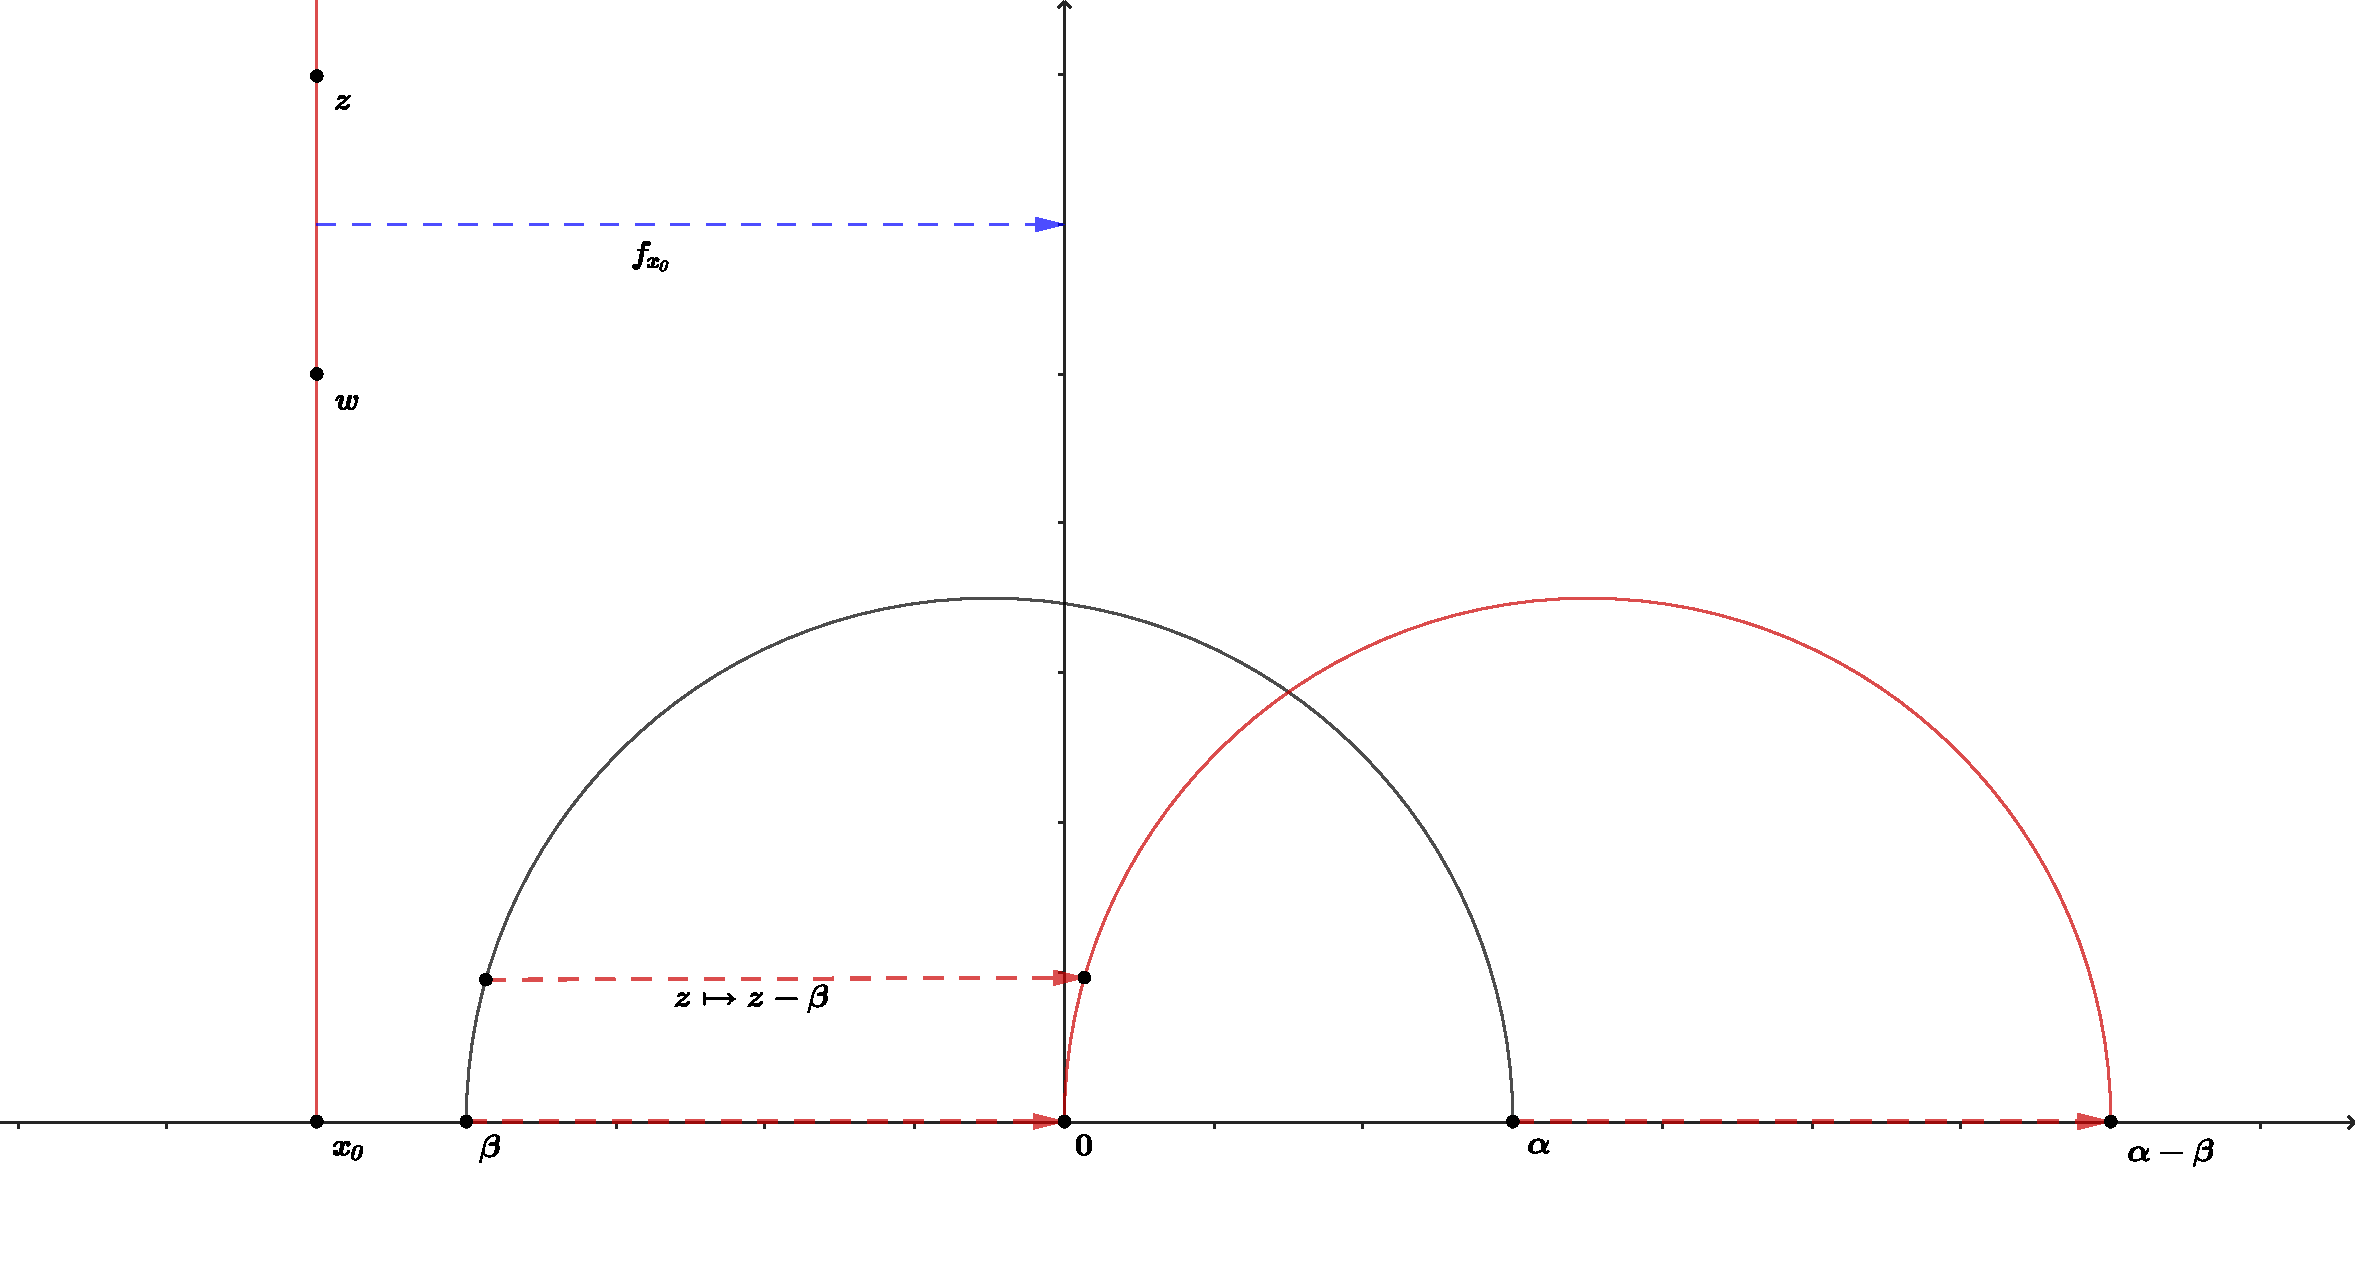
\includegraphics[width=0.75\linewidth]{images/Đường hyperbolic biến thành trục ảo.pdf}
%         \caption{Đường hyperbolic biến thành trục ảo}
%         \label{Đường hyperbolic biến thành trục ảo}
%     \end{figure}
    
%     Xét đường thẳng hyperbolic $\Axis(x_0) = \{x_0 +iy~|~y>0\}\subset \hh$.
    
%     Xét phép biến đổi $T_{x_0}:z \mapsto z-x_0$ trong $\PSL(2,\R)$. Ta có
%     \[T_{x_0}(\Axis(x_0)) = \{T_{x_0}(z)~|~z\in \Axis(x_0)\} = \{(x_0+iy)-x_0 ~|~y>0\}=\{iy ~|~y>0\} = \Axis(0).\]
%     Xét nửa đường tròn hyperbolic $\Cir(\alpha,\beta)$ trong $\hh$.
    
%     Giả sử $\alpha >\beta$, khi đó $\Cir(\alpha,\beta)$ là nửa đường tròn tâm $c = \dfrac{\alpha+\beta}{2}$ và bán kính $r = \dfrac{\alpha - \beta}{2}$. 

%     Với mọi $z\in \Cir(\alpha,\beta)$ thì $\left|z-c\right|= r$, tức là $z = c + re^{i\phi}, \phi \in (0,\pi)$.

%     Xét phép biến đổi $T_{\alpha, \beta}: z\mapsto \dfrac{z-\alpha}{z-\beta}$ trong $\PSL(2,\R)$.
%     Ta có 
%     \begin{align*}
%     T_{\alpha,\beta}(c + re^{i\phi}) &= \dfrac{\dfrac{\alpha - \beta}{2}e^{i\phi}-\dfrac{\alpha - \beta}{2}}{\dfrac{\alpha - \beta}{2}e^{i\phi}+\dfrac{\alpha - \beta}{2}} = \dfrac{e^{i\phi}-1}{e^{i\phi}+1} = \dfrac{(\cos\phi-1)+i\sin\phi}{(\cos\phi+1)+i\sin\phi}\\
%     &= \dfrac{-2\sin^2(\phi/2) + 2i\sin(\phi/2)\cos(\phi/2)}{2\cos^2(\phi/2) + 2i\sin(\phi/2)\cos(\phi/2)}\\
%     &= \dfrac{2i\sin(\phi/2) [\cos(\phi/2)+i\sin(\phi/2)]}{2\cos(\phi/2)[\cos(\phi/2) + i\sin(\phi/2)]}\\
%     & = \tan(\phi/2)i
%     \end{align*}
%     Do đó $T_{\alpha,\beta}(\Cir(\alpha,\beta)) = \left\{\tan(\phi/2)i~|~\phi \in (0,\pi)\right\} =\{it~|~t\in \R_{>0}\} = \Axis(0)$, vì với mỗi $t>0$ có một và chỉ một $\phi \in (0,\pi)$ sao cho $t = \tan(\phi/2).$
% \end{proof}
% \begin{thm}
%     Đoạn trắc địa nối 2 điểm phân biệt $z,w$ trong $\hh$ đều nằm trong đường hyperbolic duy nhất đi qua chúng.
% \end{thm}
% \begin{proof}
%     Xét hai điểm phân biệt $z,w \in \hh$. Khi đó tồn tại duy nhất một đường hyperbolic đi qua $z,w$, gọi là $l_{z,w}$. Theo bổ đề \ref{lem 2.2.4} thì tồn tại một phép biến đổi $T \in \PSL(2,\R)$ biến $l_{z,w}$ thành trục ảo $\Axis(0)$. Giả sử $T(z) = ia, T(w) = ib$ với $0<a<b$.

%     Theo mệnh đề \ref{prop 2.1.8} kết hợp với $T$ là một đẳng cự trong $\hh$ ta được $\rho(z,w) = \rho(T(z),T(w)) = \rho(ia,ib) = \ln{\dfrac{b}{a}}$. Tức đoạn trắc địa giữa $T(z)$ và $T(w)$ chính là
%     là đoạn thẳng Euclid nối $ia, ib$ trên trục ảo chính.

%     Dẫn đến đoạn trắc địa nối $z,w$ phải nằm trên $l_{z,w}$.
    
% \end{proof}
%-------------------------------------------------------------------------
% \begin{lem}
%     Với $z,w \in \hh$ và $f \in \PSL(2,\R)$, ta có
%     \[|f(z)-f(w)| = |z-w|\big|f'(z)f'(w)\big|^{1/2}\]
% \end{lem}
% \begin{proof}
%     Lấy bất kỳ $f\in \PSL(2,\R),~f(z) = \dfrac{az+b}{cz+d}~(ad-bc=1)$, khi đó với mọi $z,w \in \hh$, ta được 
%         \[|f(z) - f(w)| = \dfrac{|z-w|}{|(cz+d)(cw+d)|}.\]
%     Mà $f'(z) = \dfrac{1}{(cz+d)^2}$ và $f'(w) = \dfrac{1}{(cw+d)^2}$ nên
%     $|f(z)-f(w)| = |z-w|\big|f'(z)f'(w)\big|^{1/2}$.
% \end{proof}
%-------------------------------------------------------------------------
Tiếp theo ta có công thức liên quan đến khoảng cách hyperbolic cho 2 điểm bất kỳ trên $\hh$.
\begin{thm}\label{thm 2.2.4}
    Với $z,w \in \hh$, ta có các đẳng thức sau
    \begin{enumerate}
        \item $\rho(z,w) = \ln{\dfrac{|z-\overline{w}|+|z-w|}{|z-\overline{w}|-|z-w|}}$,
        \item $\cosh\rho(z,w) = 1 + \dfrac{|z-w|^2}{2\im(z)\im(w)}$,
        \item $\sinh\left(\dfrac{1}{2}\rho(z,w)\right) = \dfrac{|z-w|}{2(\im(z)\im(w))^{1/2}}$,
        \item $\cosh\left(\dfrac{1}{2}\rho(z,w)\right) = \dfrac{|z-\overline{w}|}{2(\im(z)\im(w))^{1/2}}$,
        \item $\tanh\left(\dfrac{1}{2}\rho(z,w)\right) = \dfrac{|z-w|}{|z-\overline{w}|}\cdot$
    \end{enumerate}
\end{thm}
\begin{proof}
    Lấy bất kỳ $z,w \in \hh$.

    Nếu $z = w$ thì hiển nhiên các đẳng thức cần chứng minh là thoả mãn.
    
    Nếu $z \neq w$, khi đó tồn tại phép biến đổi $f(z) = \dfrac{az+b}{cz+d}$ trong $\PSL(2,\R)$ sao cho 
        \[f(z) = iu,~f(w)=iv~(u>v>0).\]
    Vì $f$ cũng là một đẳng cự nên \[\rho(z,w) = \rho(f(z),f(w)) = \rho(iu,iv) = \ln{\dfrac{u}{v}}\cdot\]
    Do đó
    \[\exp{(\rho(z,w))} =  \dfrac{u}{v},~\exp{(-\rho(z,w))} = \dfrac{v}{u},\]
    \[\exp{\left(\dfrac{1}{2}\rho(z,w)\right)} = \sqrt{\dfrac{u}{v}},~\exp{\left(-\dfrac{1}{2}\rho(z,w)\right)}  = \sqrt{\dfrac{v}{u}}.\]
    Ta lần lượt tính các vế trái của 5 ý trên như sau
    \begin{align*}
         \cosh\rho(z,w) &= \dfrac{\dfrac{u}{v}+\dfrac{v}{u}}{2} = \dfrac{u^2+v^2}{2uv},\\
         \sinh\left(\dfrac{1}{2}\rho(z,w)\right) &= \dfrac{\sqrt{\dfrac{u}{v}}-\sqrt{\dfrac{v}{u}}}{2} = \dfrac{u-v}{2\sqrt{uv}},\\
         \cosh\left(\dfrac{1}{2}\rho(z,w)\right) &= \dfrac{\sqrt{\dfrac{u}{v}}+\sqrt{\dfrac{v}{u}}}{2} = \dfrac{u+v}{2\sqrt{uv}},\\
         \tanh\left(\dfrac{1}{2}\rho(z,w)\right) & = \dfrac{\sinh\left(\dfrac{1}{2}\rho(z,w)\right)}{\cosh\left(\dfrac{1}{2}\rho(z,w)\right)} = \dfrac{u-v}{u+v}.
    \end{align*}
    Tiếp theo ta sẽ tính các vế phải của 5 ý cần chứng minh. 
    
    Ta có $f^{-1}(z) = \dfrac{dz-b}{-cz+a},~\im(f^{-1}(z)) = \dfrac{\im(z)}{|-cz+a|^2}\cdot$
    
    Vì vậy, ta thu được 
    \begin{align*}
        z &= f^{-1}(iu) =\dfrac{-b+i(du)}{a-i(cu)},~\overline{z} =\dfrac{-b-i(du)}{a+i(cu)}\cdot\\
        w &= f^{-1}(iv) =\dfrac{-b+i(dv)}{a-i(cv)},~\overline{w} =\dfrac{-b-i(dv)}{a+i(cv)}\cdot\\
        \im(z) &= \dfrac{u}{a^2+(cu)^2},\quad
        \im(w) = \dfrac{v}{a^2+(cv)^2}\cdot\\
        |z-w|  &= \dfrac{|u-v|}{\sqrt{(a^2+(cu)^2)(a^2+(cv)^2)}},\\
        |z-\overline{w}|  & =\dfrac{|u+v|}{\sqrt{(a^2+(cu)^2)(a^2+(cv)^2)}}\cdot
    \end{align*}
    Ta có các vế phải của 5 ý cần chứng minh lần lượt là 
    \begin{enumerate}
        \item \[\ln{\dfrac{|z-\overline{w}|+|z-w|}{|z-\overline{w}|-|z-w|}}
            = \ln{\dfrac{|u+v|+|u-v|}{|u+v|-|u-v|}}
            = \ln{\dfrac{u}{v}} = \rho(z,w)(\text{do }u>v>0).\]
        % \end{align*}
        \item \[1 + \dfrac{|z-w|^2}{2\im(z)\im(w)} = 1 + \dfrac{|u-v|^2}{2uv} = 1 + \dfrac{(u-v)^2}{2uv} = \dfrac{u^2+v^2}{2uv} = \cosh{\rho(z,w)}.\]
        % \end{align*}
        \item \[\dfrac{|z-w|}{2(\im(z)\im(w))^{1/2}}= \dfrac{u-v}{2\sqrt{uv}} = \sinh\left(\dfrac{1}{2}\rho(z,w)\right).\]
        \item \[\dfrac{|z-\overline{w}|}{2(\im(z)\im(w))^{1/2}}= \dfrac{u+v}{2\sqrt{uv}} = \cosh\left(\dfrac{1}{2}\rho(z,w)\right).\]
        \item \[\dfrac{|z-w|}{|z-\overline{w}|}=\dfrac{u-v}{u+v} = \tanh\left(\dfrac{1}{2}\rho(z,w)\right).\]
    \end{enumerate}
    Từ đó ta có điều phải chứng minh.
\end{proof}
\begin{remark*}
    Từ định lý trên ta thấy, nếu $z_1\neq z_2$ thì $\rho(z_1,z_2) >0$. Điều này kết hợp với những chứng minh ở mệnh đề \ref{prop 2.1.7} nói rằng $\rho$ là một metric trên $\hh$.
\end{remark*}

% \subsection{Đoạn trắc địa}
% \begin{defn}[Đoạn trắc địa]
%     \textbf{Đoạn trắc địa} giữa hai điểm $z,w$ trong $\hh$ là đường cong  có \textit{độ dài hyperbolic ngắn nhất} nối $z$ và $w$, được ký hiệu là $[z,w]$.
    
%     % Khoảng cách của $z,w$ được đo bằng độ dài hyperbolic của đoạn trắc địa đó.
% \end{defn}
% \begin{thm}
%     Đoạn trắc địa nối 2 điểm phân biệt $z,w$ trong $\hh$ đều nằm trong đường hyperbolic duy nhất đi qua chúng.
% \end{thm}
% \begin{proof}
%     Xét hai điểm phân biệt $z,w \in \hh$. Khi đó tồn tại duy nhất một đường hyperbolic đi qua $z,w$, gọi là $l_{z,w}$. Theo bổ đề \ref{lem 2.2.4} thì tồn tại một phép biến đổi $T \in \PSL(2,\R)$ biến $l_{z,w}$ thành trục ảo $\Axis(0)$. Giả sử $T(z) = ia, T(w) = ib$ với $0<a<b$.

%     Theo mệnh đề \ref{prop 2.1.8} kết hợp với $T$ là một đẳng cự trong $\hh$ ta được $\rho(z,w) = \rho(T(z),T(w)) = \rho(ia,ib) = \ln{\dfrac{b}{a}}$. Tức đoạn trắc địa giữa $T(z)$ và $T(w)$ chính là
%     là đoạn thẳng Euclid nối $ia, ib$ trên trục ảo chính.

%     Dẫn đến đoạn trắc địa nối $z,w$ phải nằm trên $l_{z,w}$.
    
% \end{proof}
% %-------------------------------------------------------------------------
% \begin{cor}
%     Khoảng cách hyperbolic giữa $z,w$ bằng độ dài hyperbolic của đoạn trắc địa duy nhất nói trên.
% \end{cor}
%-------------------------------------------------------------------------
\begin{lem}\label{lem 2.2.6}
    Cho $\gamma:[0,1]\to \hh,~\gamma(t) = u(t) + iv(t),~\gamma(0) = ia,~\gamma(1) = c+ib$ là đường cong trơn từng khúc nối $ia,~c+ib ~(c\neq 0<a,b)$ và $\phi:[0,1]\to \hh,~\phi(t) =iv(t)$ là một đường cong trơn từng khúc nối $ia,~ib$. Khi đó $h(\gamma) > h(\phi)$.
\end{lem}
\begin{proof}
    Ta có $\phi(t)=iv(t)$ nên $\im(\phi(t)) = v(t)$ và $|\phi'(t)|=|v'(t)|$. Khi đó
    \begin{align*}
        h(\gamma) = \int_{0}^{1}{\dfrac{\sqrt{(u'(t))^2+(v'(t))^2}}{v(t)}}dt 
        > \int_{0}^{1}{\dfrac{\left|v'(t)\right|}{v(t)}}dt 
        = \int_{0}^{1}{\dfrac{|\phi'(t)|}{\im(\phi(t))}}dt 
        = h(\phi).
    \end{align*}
    % Từ đó suy ra $\rho(ia,ib) < \rho(ia, c+ib)$
\end{proof}
%-------------------------------------------------------------------------
\begin{lem}\label{lem 2.2.7}  
    Cho $z = c+ib,~w=ia \in \hh,~c\neq 0<a,b$. Khi đó $\rho(c+ia, ib) > \rho(ia,ib)$.
\end{lem}
\begin{proof}
     Với $z=c+ib,~w=ia,~c\neq 0<a,b,~b\neq a$ ta được 
    \begin{align*}
        \rho(c+ib,ia) &= \ln{\dfrac{|(c+ib)-(-ia)|+|(c+ib)-(ia)|}{|(c+ib)-(-ia)|-|(c+ib)-(ia)|}}\\
        &= \ln{\dfrac{\sqrt{c^2+(b+a)^2} + \sqrt{c^2+(b-a)^2}}{\sqrt{c^2+(b+a)^2} - \sqrt{c^2+(b-a)^2}}}
    \end{align*}
    \begin{itemize}
        \item Nếu $b=a$ thì \[\rho(c+ib,ia)=\rho(c+ia,ia) = \ln{\dfrac{\sqrt{c^2+(2a)^2} + \sqrt{c^2}}{\sqrt{c^2+(2a)^2} - \sqrt{c^2}}} > \ln{1} = 0 = \rho(ia,ia).\]
        \item Nếu $b\neq a$, do $f(x) = \ln\dfrac{x+1}{x-1},~x>1$ có $f'(x) = \dfrac{-2}{x^2-1} < 0 ~\forall x>1$, nên $f$ là hàm giảm. Do đó với $1<\sqrt{\dfrac{c^2+(b+a)^2}{c^2+(b-a)^2}} < \sqrt{\dfrac{(b+a)^2}{(b-a)^2}}$ thì \[\rho(c+ib,ia)=f\left(\sqrt{\dfrac{c^2+(b+a)^2}{c^2+(b-a)^2}}\right) > f\left(\sqrt{\dfrac{(b+a)^2}{(b-a)^2}}\right) = \rho(ib,ia).\]
    \end{itemize}
\end{proof}
%-------------------------------------------------------------------------
\begin{prop}\label{prop 2.2.8}
    Cho $z,w$ là hai điểm phân biệt trong $\hh$. Khi đó $\rho(z,w) = \rho(z,\xi) + \rho(\xi,w)$ nếu và chỉ nếu $\xi \in [z,w]$.
\end{prop}
\begin{proof}
    Với $z,w \in \hh$ phân biệt, tồn tại phép biến đổi $f \in \PSL(2,\R)$ sao cho \[f(z) = ia,~f(w)= ib~\text{ với } b>a>0 \text{ và } \rho(z,w) =\rho(f(z),f(w)) =\rho(ia,ib)=\ln{\dfrac{b}{a}}\cdot\]
    \begin{figure}[!htp]
        \centering
        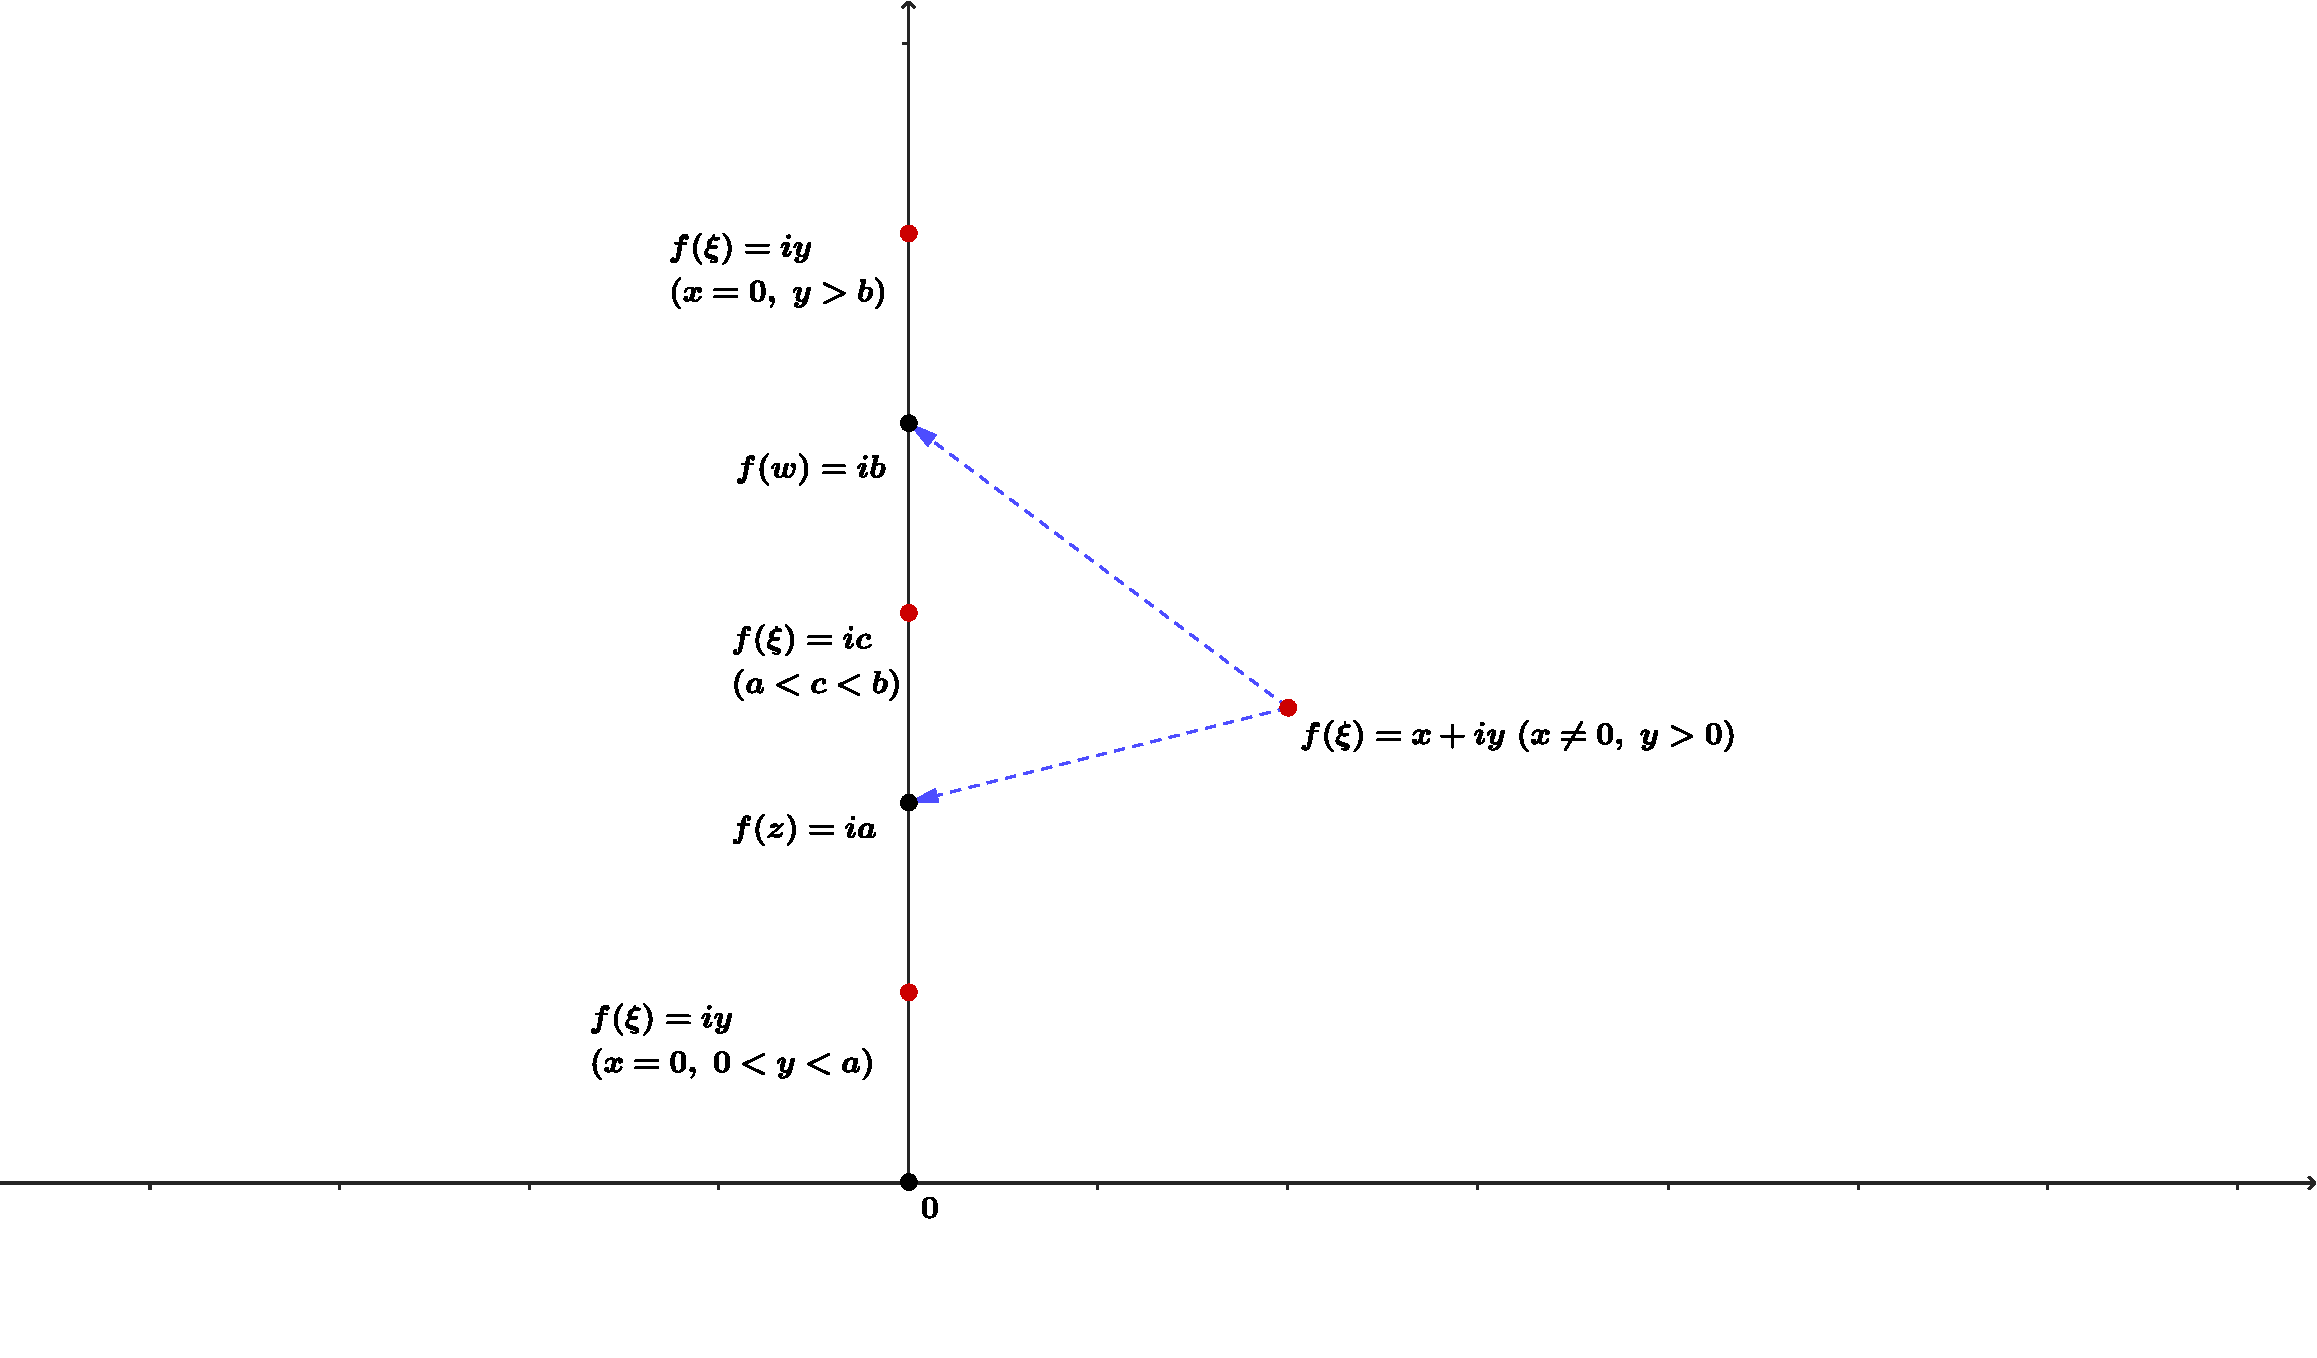
\includegraphics[width=0.6\linewidth]{images/hinh_1.2.1.pdf}
        % \caption{}
        % \label{}
    \end{figure}
    \begin{enumerate}
        \item Nếu $\xi \in [z,w]$ thì $f(\xi) \in [f(z),f(w)]$ nên tồn tại $a<c<b$ sao cho $f(\xi) = ic$. Khi đó 
        \[\rho(z,\xi) = \ln{\dfrac{c}{a}},~\rho(\xi,w) = \ln{\dfrac{b}{c}}\cdot\]
        Suy ra $ \rho(z,\xi) + \rho(\xi,w) = \ln{\dfrac{c}{a}} + \ln{\dfrac{b}{c}} = \ln{\dfrac{b}{a}} = \rho(z,w)$.
        \item Ngược lại, nếu $\rho(z,w) = \rho(z,\xi) + \rho(\xi,w)$, ta cần chứng minh $\xi \in [z,w]$. Giả sử phản chứng $\xi \notin [z,w]$. Đặt $f(\xi) = x+iy~(y>0)$.
        \begin{itemize}
            \item[i)] Nếu $x = 0$ thì $f(\xi) = iy $, do $f$ là song ánh nên $ f(\xi)$ khác $f(z) = ia,~f(w)=ib$, tức $y \neq a,b$, nghĩa là $y > b$ hoặc $0<y<a$. 
            \begin{itemize}
                \item Nếu $y>b$ thì $\rho(z,\xi) + \rho(\xi,w) - \rho(z,w) = \ln{\dfrac{y}{a}} + \ln{\dfrac{y}{b}} - \ln{\dfrac{b}{a}}= \ln{\dfrac{y^2}{b^2}} > \ln{1}=0$.
                \item Nếu $0<y<a$ thì $\rho(z,\xi) + \rho(\xi,w) - \rho(z,w) = \ln{\dfrac{a}{y}} + \ln{\dfrac{b}{y}} - \ln{\dfrac{b}{a}}= \ln{\dfrac{a^2}{y^2}}>\ln{1}=0$.
            \end{itemize}
            Cả hai trường hợp này đều mâu thuẫn với $\rho(z,w) = \rho(z,\xi) + \rho(\xi,w)$.
            \item[ii)] Nếu $x\neq 0$ thì $f(\xi) = x+iy$ không thuộc trục ảo, do đó $f(\xi) \notin [ia,ib]=[f(z),f(w)]$. Khi đó áp dụng bổ đề \ref{lem 2.2.7}
            \begin{itemize}
                \item Nếu $a\leq y \leq b$ thì 
                \begin{align*}
                    \rho(z,\xi) + \rho(\xi,w) - \rho(z,w) &= \rho(ia,x+iy) + \rho(x+iy,ib) - \rho(ia,ib)\\
                    &> \rho(ia,iy) + \rho(iy,ib) -\rho(ia,ib)\\
                    &=\ln{\dfrac{y}{a}} + \ln{\dfrac{b}{y}} - \ln{\dfrac{b}{a}} = 0.
                \end{align*}
                \item Nếu $0<y<a<b$ thì 
                \begin{align*}
                    \rho(z,\xi) + \rho(\xi,w) - \rho(z,w) &= \rho(ia,x+iy) + \rho(x+iy,ib) - \rho(ia,ib)\\
                    &> \rho(ia,iy) + \rho(iy,ib) -\rho(ia,ib)\\
                    &=\ln{\dfrac{a}{y}} + \ln{\dfrac{b}{y}} - \ln{\dfrac{b}{a}} = \ln{\dfrac{a^2}{y^2}} > \ln{1} = 0.
                \end{align*}
                \item Nếu $y>b$
                \begin{align*}
                    \rho(z,\xi) + \rho(\xi,w) - \rho(z,w) &= \rho(ia,x+iy) + \rho(x+iy,ib) - \rho(ia,ib)\\
                    &> \rho(ia,iy) + \rho(iy,ib) -\rho(ia,ib)\\
                    &=\ln{\dfrac{y}{a}} + \ln{\dfrac{y}{b}} - \ln{\dfrac{b}{a}} = \ln{\dfrac{y^2}{b^2}} > \ln{1} = 0.
                \end{align*}
            \end{itemize}
            Cả 3 trường hợp này đều mâu thuẫn với $\rho(z,w) = \rho(z,\xi) + \rho(\xi,w)$.
        \end{itemize}
        Chứng tỏ giả sử phản chứng là sai. Vì vậy $\xi \in [z,w]$.
    \end{enumerate}
\end{proof}
%-------------------------------------------------------------------------
% \begin{prop}\label{prop 2.2.9}
%     Mọi phép biến đổi trong $\PSL(2,\R)$ biến đoạn trắc địa thành đoạn trắc địa trong $\hh$.
% \end{prop}
% \begin{proof}
%     Giả sử $f \in \PSL(2,\R)$ và $z,w$ là hai điểm bất kỳ trong $\hh$ được nối bởi đoạn trắc địa $l = [z,w]$. Khi đó ta cần chỉ ra $f$ tác động lên $l$ thành một đoạn trắc địa trong $\hh$. 
    
%     Thật vậy, với mọi $\xi \in l$ thì 
%     \[\rho(z,w) = \rho(z,\xi) + \rho(\xi,w).\]
%     Mà $f$ là một đẳng cự trong $\hh$ nên
%     \[\rho(f(z),f(w)) =\rho(z,w) = \rho(z,\xi) + \rho(\xi,w)= \rho(f(z),f(\xi)) + \rho(f(\xi),f(w)).\] 
%     Điều này xảy ra khi và chỉ khi $f(\xi) \in [f(z), f(w)]$ là đoạn trắc địa nối $f(z),f(w)$. 
    
%     Chứng tỏ $\forall \xi \in [z,w]$ thì $f(\xi) \in [f(z), f(w)]$, nghĩa là $f$ biến đoạn trắc địa thành đoạn trắc địa trong $\hh$.
% \end{proof}
% \begin{cor}
%     Đoạn trắc địa nối 2 điểm phân biệt $z,w$ trong $\hh$ đều nằm trong đường hyperbolic duy nhất đi qua chúng.
% \end{cor}
% \begin{proof}
%     Xét hai điểm phân biệt $z,w \in \hh$. Khi đó tồn tại duy nhất một đường hyperbolic đi qua $z,w$, gọi là $l_{z,w}$. Tồn tại một phép biến đổi $T \in \PSL(2,\R)$ biến $l_{z,w}$ thành trục ảo $\Axis(0)$. 
    
%     Giả sử $T(z) = ia, T(w) = ib$ với $0<a<b$.
%     Mà đoạn thẳng Euclid nối $ia,ib$ trên trục ảo là đoạn có độ dài hyperbolic nhỏ nhất nối $ia,ib$, cụ thể $\rho(ia,ib) = \ln\dfrac{b}{a}$. 
    
%     Nên đoạn trắc địa $[T(z),T(w)]\subset T(l_{z,w})$ chính là đoạn thẳng Euclid nói trên. Đoạn thẳng này qua ánh xạ nghịch đảo $T^{-1}$ thuộc $l_{z,w}$.
    
%     Mà $T^{-1} \in \PSL(2,\R)$ nên biến đoạn trắc địa thành đoạn trắc địa, 
%     nên $[T^{-1}(ia),T^{-1}(ib)]$ chính là đoạn trắc địa qua $z,w$. 
    
%     Chứng tỏ $[z,w] \in l_{z,w}$.
% \end{proof}
% \begin{remark*}
%     Từ đây, ta thấy mọi đoạn trắc địa đều nằm trên một đường hyperbolic nào đó. Do đó, ta còn gọi đường hyperbolic là đường trắc địa.
% \end{remark*}
% %-------------------------------------------------------------------------
% \begin{cor}
%     Khoảng cách hyperbolic giữa $z,w \in \hh$ bằng độ dài hyperbolic của đoạn trắc địa qua chúng.
% \end{cor}
%-------------------------------------------------------------------------
\subsubsection{Tỉ số kép}
\begin{defn}[Tỉ số kép]
    \textbf{Tỉ số kép} của bốn điểm phân biệt $[z_1:w_1],[z_2:w_2],[z_3:w_3],[z_4:w_4]$ trên đường thẳng xạ ảnh $P^1(\C)$ là 

    \[([z_1:w_1],[z_2:w_2];[z_3:w_3],[z_4:w_4]) = \dfrac{\begin{vmatrix}
         z_1 & z_2\\
         w_1 & w_2
    \end{vmatrix}\begin{vmatrix}
         z_3 & z_4\\
         w_3 & w_4
    \end{vmatrix}}{\begin{vmatrix}
         z_2 & z_3\\
         w_2 & w_3
    \end{vmatrix}\begin{vmatrix}
         z_4 & z_1\\
         w_4 & w_1
    \end{vmatrix}}\in \C\]
\end{defn}
\begin{exam*}
    Tỉ số kép của bốn điểm phân biệt $z_1,z_2,z_3,z_4 \in \C$ là 
    \begin{align*}
        (z_1,z_2;z_3,z_4) &= \dfrac{\begin{vmatrix}
         z_1 & z_2\\
         1 & 1
    \end{vmatrix}\begin{vmatrix}
         z_3 & z_4\\
         1 & 1
    \end{vmatrix}}{\begin{vmatrix}
         z_2 & z_3\\
         1 & 1
    \end{vmatrix}\begin{vmatrix}
         z_4 & z_1\\
         1 & 1
    \end{vmatrix}}
    = \dfrac{(z_1-z_2)(z_3-z_4)}{(z_2-z_3)(z_4-z_1)}\cdot
    \end{align*}
\end{exam*}
\begin{exam*}
    Cho bốn số phức phân biệt $z_1,z_2,z_3,z_4$.
    \begin{enumerate}
        \item Tỉ số kép của bốn điểm $\infty, z_2,z_3,z_4$ là 
        \[(\infty, z_2;z_3,z_4) = ([1:0],[z_2:1];[z_3:1],[z_4:1])=\dfrac{\begin{vmatrix}
         1 & z_2\\
         0 & 1
    \end{vmatrix}\begin{vmatrix}
         z_3 & z_4\\
         1 & 1
    \end{vmatrix}}{\begin{vmatrix}
         z_2 & z_3\\
         1 & 1
    \end{vmatrix}\begin{vmatrix}
         z_4 & 1\\
         1 & 0
    \end{vmatrix}} = \dfrac{(z_3-z_4)}{(z_3-z_2)}.\]

    \item Tỉ số kép của bốn điểm $z_1,\infty,z_3,z_4$ là 
        \[(z_1,\infty;z_3,z_4) = ([z_1:1],[1:0];[z_3:1],[z_4:1])=\dfrac{\begin{vmatrix}
         z_1 & 1\\
         1 & 0
    \end{vmatrix}\begin{vmatrix}
         z_3 & z_4\\
         1 & 1
    \end{vmatrix}}{\begin{vmatrix}
         1 & z_3\\
         0 & 1
    \end{vmatrix}\begin{vmatrix}
         z_4 & z_1\\
         1 & 1
    \end{vmatrix}} = \dfrac{(z_4-z_3)}{(z_4-z_1)}.\]

    \item Tỉ số kép của bốn điểm $z_1,z_2,\infty,z_4$ là 
        \[(z_1,z_2;\infty,z_4) = ([z_1:1],[z_2:1];[1:0],[z_4:1])=\dfrac{\begin{vmatrix}
         z_1 & z_2\\
         1 & 1
    \end{vmatrix}\begin{vmatrix}
         1 & z_4\\
         0 & 1
    \end{vmatrix}}{\begin{vmatrix}
         z_2 & 1\\
         1 & 0
    \end{vmatrix}\begin{vmatrix}
         z_4 & z_1\\
         1 & 1
    \end{vmatrix}} = \dfrac{(z_1-z_2)}{(z_1-z_4)}.\]

    \item Tỉ số kép của bốn điểm $z_1,z_2,z_3,\infty$ là 
        \[(z_1,z_2;z_3,\infty) = ([z_1:1],[z_2:1];[z_3:1],[1:0])=\dfrac{\begin{vmatrix}
         z_1 & z_2\\
         1 & 1
    \end{vmatrix}\begin{vmatrix}
         z_3 & 1\\
         1 & 0
    \end{vmatrix}}{\begin{vmatrix}
         z_2 & z_3\\
         1 & 1
    \end{vmatrix}\begin{vmatrix}
         1 & z_1\\
         0 & 1
    \end{vmatrix}} = \dfrac{(z_2-z_3)}{(z_2-z_1)}.\]
    \end{enumerate}
\end{exam*}

\begin{prop}\label{prop 2.2.15}
    Các phép biến đổi phân tuyến tính của $P^1(\C)$ bảo toàn tỉ số kép. Cụ thể hơn, với bốn điểm phân biệt $P_1,P_2,P_3,P_4$ và phép biến đổi phân tuyến tính $T$ của $P^1(\C)$, ta có
    \[(P_1,P_2;P_3,P_4) = (T(P_1),T(P_2);T(P_3),T(P_4)).\]
\end{prop}
\begin{proof}
    Giả sử $T$ là phép biến đổi phân tuyến tính ứng với ma trận $A\in \GL(2,\C)$. 
    
    Đặt $P_j=[z_j:w_j]$ với $j=1,2,3,4$. Khi đó $T(P_j) = [z'_j:w'_j]$, trong đó $\begin{bmatrix}
        z_j' \\
        w_j'
    \end{bmatrix} = A\begin{bmatrix}
        z_j \\
        w_j
    \end{bmatrix}$.

    Dẫn đến $\begin{bmatrix}
        z_j' & z_k'\\
        w_j' & w_k'
    \end{bmatrix} = A\begin{bmatrix}
        z_j & z_k\\
        w_j & w_k
    \end{bmatrix}$. Do đó $\begin{vmatrix}
        z_j' & z_k'\\
        w_j' & w_k'
    \end{vmatrix} = \det(A)\begin{vmatrix}
        z_j & z_k\\
        w_j & w_k
    \end{vmatrix}$.

    Vì vậy 
    \begin{align*}
        (T(P_1),T(P_2);T(P_3),T(P_4)) &= ([z_1':w_1'],[z_2':w_2'];[z_3':w_3'],[z_4':w_4'])\\
        &= \dfrac{\begin{vmatrix}
         z_1' & z_2'\\
         w_1' & w_2'
    \end{vmatrix}\begin{vmatrix}
         z_3' & z_4'\\
         w_3' & w_4'
    \end{vmatrix}}{\begin{vmatrix}
         z_2' & z_3'\\
         w_2' & w_3'
    \end{vmatrix}\begin{vmatrix}
         z_4' & z_1'\\
         w_4' & w_1'
    \end{vmatrix}}
    = \dfrac{\det(A)\begin{vmatrix}
         z_1 & z_2\\
         w_1 & w_2
    \end{vmatrix}\det(A)\begin{vmatrix}
         z_3 & z_4\\
         w_3 & w_4
    \end{vmatrix}}{\det(A)\begin{vmatrix}
         z_2 & z_3\\
         w_2 & w_3
    \end{vmatrix}\det(A)\begin{vmatrix}
         z_4 & z_1\\
         w_4 & w_1
    \end{vmatrix}}\\
    &= ([z_1:w_1],[z_2:w_2];[z_3:w_3],[z_4:w_4])\\
    &=(P_1,P_2;P_3,P_4).
    \end{align*}
\end{proof}
%-------------------------------------------------------------------------
\begin{thm}\label{thm 2.2.16}
    Cho $z_1\neq z_2$ trong $\hh$. Kí hiệu $z_1^*,z_2^* \in \R \cup \{\infty\}$ là hai giao điểm của đường hyperbolic duy nhất qua $z_1^*,z_2^*$ với $\R \cup \{\infty\}$. Khi đó
    \[\rho(z_1,z_2) = |\ln{(z_2,z_1^*~;~z_1,z_2^*)}|.\]
\end{thm}
\begin{proof}
    Vì $z_1 \neq z_2$ nên tồn tại duy nhất một đường hyperbolic qua $z_1,z_2$ là $h-line(z_1^*,z_2^*)$ với $z_1^*,z_2^*$ là giao điểm với $\R\cup\{\infty\}$. Ta có hai trường hợp sau
    \begin{enumerate}
        \item $z_1^*,z_2^* \in \R,~z_1^*<z_2^*$.

        Xét phép biến đổi $f(z) = \dfrac{z-z_2^*}{z-z_1^*}$ trong $\PSL(2,\R)$ biến $h-line(z_1^*,z_2^*)$ thành $h-line(0,\infty)$. 
        
        Giả sử $f(z_1) = ia, f(z_2) = ib$ với $a,b>0$.
        

        Phép biến đổi này cảm sinh một phép biến đổi xạ ảnh
        \[P^1(\C) \to P^1(\C),\quad [z:w]\mapsto [z-z_2^*w:z-z_1^*w].\]
        Nói riêng 
            $[z_1^*:1]\mapsto [z_1^*-z_2^*:0] = [1:0] \quad
            [z_2^*:1]\mapsto [0:z_2^*-z_1^*] = [0:1]$
        
        Do $f_{z_1,z_2}$ bảo toàn tỉ số kép nên
        \begin{align*}
         (z_2,z_1^*~;~z_1,z_2^*) 
         &= (f([z_2:1]),f([z_1^*:1]);f([z_1:1]),f([z_2^*:1])) \\
         &= ([f(z_2):1],[1,0];[f(z_1):1],[0:1])\\
         % &= ([|f(z_2)|:1],[1,0];[|f(z_1)|:1],[0:1])\\
         &= \dfrac{0-f(z_1)}{0-f(z_2)} = \dfrac{ia}{ib} = \dfrac{a}{b}.
        \end{align*}
        Suy ra $\rho(z_1,z_2) = \rho(f(z_1),f(z_2)) = \rho(ia,ib) = \left|\ln{\dfrac{a}{b}}\right| = |\ln{(z_2,z_1^*~;~z_1,z_2^*)}|$.

        \item Nếu $z_1^* = r \in \R, z_2^* = \infty$. Khi đó $h-line(z_1^*,z_2^*) = h-line(r,\infty)$. Ta có phép biến đổi $T(z) = z-r$ trong $\PSL(2,\R)$ biến $h-line(r,\infty)$ thành $h-line(0,\infty)$. Giả sử $T(z_1) = ia, T(z_2) = ib$ với $a,b>0$.

        Phép biến đổi $T$ cảm sinh một phép biến đổi xạ ảnh trên $P^1(\C)$ là 
        \[P^1(\C) \to P^1(\C),\quad [z:w]\mapsto [z-rw:w].\]
        Nói riêng 
            $[z_1^*:1] = [r:1]\mapsto [0:1], \quad
            [1:0]\mapsto [1:0]$
        
        Do $f_{z_1,z_2}$ bảo toàn tỉ số kép nên
        \begin{align*}
         (z_2,z_1^*~;~z_1,z_2^*) 
         &= (T([z_2:1]),T([z_1^*:1]);T([z_1:1]),T([1:0])) \\
         &= ([T(z_2):1],[0,1];[T(z_1):1],[1:0])\\
         &= \dfrac{0-T(z_1)}{0-T(z_2)} = \dfrac{ia}{ib} = \dfrac{a}{b}.
        \end{align*}
        Suy ra $\rho(z_1,z_2) = \rho(T(z_1),T(z_2)) = \rho(ia,ib) = \left|\ln{\dfrac{a}{b}}\right| = |\ln{(z_2,z_1^*~;~z_1,z_2^*)}|$.
    \end{enumerate}
    
\end{proof}

\section{Mô hình đĩa Poincare. Ánh xạ bảo giác}
\subsection{Mô hình đĩa Poincare}
\begin{defn}[Đĩa đơn vị]
    Tập $\U = \{z\in \C ~|~|z| < 1\}$ được gọi là đĩa đơn vị trong mặt phẳng phức $\C$.
\end{defn}
    Ta sẽ xây dựng các đối tượng của hình học hyperbolic trên đĩa đơn vị này và chuyển tất cả các thông tin hình học hyperbolic trong $\hh$ lên đĩa đơn vị $\U$.

\begin{lem}\label{lem 2.3.2}
    Ánh xạ $f(z) = \dfrac{iz+1}{z+i}$ là một vi phôi từ $\hh$ lên đĩa đơn vị $\U$.
\end{lem}
\begin{proof}
    Ta có $f$ là một ánh xạ phân tuyến tính khả vi với $f'(z) = \dfrac{-2}{(z+i)^2} \neq 0$ nên nó là một song ánh liên tục. Hơn nữa $f^{-1}(z) = \dfrac{iz-1}{-z+i}$ cũng là một ánh xạ khả vi trên $\overline{\C}$. 
    
    Chứng tỏ $f$ là một vi phôi trên $\C$.
     \begin{enumerate}
         \item Với mọi $z \in \hh$, tức $\im(z) >0$ thì $f(z) \in \U$.
         Thật vậy,
         \begin{align*}
            |f(z)| &=\sqrt{\left(\dfrac{iz+1}{z+i}\right)\overline{\left(\dfrac{iz+1}{z+i}\right)}}
             % = \dfrac{(iz+1)(-i\overline{z}+1)}{(z+i)(\overline{z}-i)}
             % = \dfrac{z\overline{z}+iz-i\overline{z}+1}{z\overline{z}-iz+i\overline{z}+1}
             = \sqrt{\dfrac{|z|^2-2\im(z) +1}{|z|^2+2\im(z) +1}} < 1\cdot
        \end{align*}
        % Mà $\im(z) > 0$  nên 
        % \[|z|^2+2\im(z) +1 >  (\im(z) - 1)^2 + (\re(z))^2 \geq 0, \] 
        % chứng tỏ $|f(z)|^2 < 1$, tức là $|f(z)| < 1$.
        \item Với mọi $z \in \U$, tức $|z| < 1$ thì $w=f^{-1}(z) \in \hh$. Thật vậy,
        \begin{align*}
            \im(w) = \dfrac{w - \overline{w}}{2i} 
            = \dfrac{1}{2i}\left(\dfrac{iz-1}{-z+i} - \dfrac{-i\overline{z}-1}{-\overline{z}-i}\right)
            = \dfrac{1}{|-z+i|^2} > 0.
        \end{align*}
     \end{enumerate}
    Vì vậy $f$ là một vi phôi từ $\hh$ lên đĩa đơn vị $\U$.
\end{proof}
\begin{remark*}
    Ta sẽ sử dụng vi phôi $f(z) = \dfrac{iz+1}{z+i}$ nói trên để chuyển tất cả các thông tin hình học hyperbolic của $\hh$ như metric, trắc địa, đẳng cự lên đĩa đơn vị $\U$.
\end{remark*}
\begin{defn}[Metric trên $\U$]
    Với mọi $z,w \in \U$ thì $f^{-1}(z),~f^{-1}(w) \in \hh$. Khi đó \[\rho^*(z,w) \defeq \rho(f^{-1}(z), f^{-1}(w))\]
    là một metric trên $\U$.
\end{defn}
\begin{proof}
    Ta sẽ chứng minh $\rho^*$ được định nghĩa như trên là một metric trên $\U$ bằng cách chỉ ra nó thoả mãn 3 tiên đề của một metric như sau
    \begin{enumerate}
        \item (Tính xác định dương) Với mọi $z,w \in \U$ thì $\rho^*(z,w) = \rho(f^{-1}(z), f^{-1}(w))\geq 0$, hơn nữa 
        \[\rho^*(z,w) = 0 \Leftrightarrow \rho(f^{-1}(z), f^{-1}(w)) = 0 \Leftrightarrow f^{-1}(z) = f^{-1}(w) \Leftrightarrow z = w.\]
        \item (Tính đối xứng) Do $\rho$ là một metric trên $\hh$ nên nó đối xứng, do đó vơi mọi $z, w \in \U$ thì 
        \[\rho^*(w,z) = \rho(f^{-1}(w), f^{-1}(z)) = \rho(f^{-1}(z), f^{-1}(w)) = \rho^*(z,w)\]
        \item (Bất đẳng thức tam giác) Với mọi $z,w,u \in \U$ thì 
        \[\rho(f^{-1}(z), f^{-1}(w)) + \rho(f^{-1}(w), f^{-1}(u)) \geq \rho(f^{-1}(z), f^{-1}(u)).\]
        Tức $\rho^*(z,w) + \rho^*(w,u) \geq \rho^*(z,u).$
    \end{enumerate}
\end{proof}
% \begin{defn}(Độ dài hyperbolic trong $\U$)
% \end{defn}
% \begin{lem}
%     Với $z \in \hh$ và $f(z) = \dfrac{zi+1}{z+i}$ thì $\dfrac{2|f'(z)|}{1-|f(z)|^2}=\dfrac{1}{\im(z)}\cdot$
% \end{lem}
% \begin{proof}
%     Ta có $f'(z) = \dfrac{-2}{(z+i)^2}$ nên 
%     \[|f'(z)| = \left|\dfrac{-2}{(z+i)^2}\right| =\dfrac{2}{|z|^2+2\im(z)+1}\cdot\] 
%     Kết hợp 
%     \[
%         \left|f(z)\right|^2 = \left|\dfrac{zi+1}{z+i}\right|^2 
%         % = \left|\dfrac{z-i}{z+i}\right|^2 
%         % = \left(\dfrac{z-i}{z+i}\right)\left(\dfrac{\overline{z}+i}{\overline{z}-i}\right)
%         = \dfrac{|z|^2-2\im(z)+1}{|z|^2+2\im(z)+1},
%     \]
%     ta được 
%     \[
%         \dfrac{2|f'(z)|}{1-|f(z)|^2} =\dfrac{1}{\im(z)}\cdot
%     \]
% \end{proof}
\begin{lem}\label{lem 2.3.4}
    Trong $\U$ thì với $0 < r< 1$ thì 
    \[\rho^*(0, ir)= \ln{\dfrac{1+r}{1-r}}\cdot\]
\end{lem}
\begin{proof}
    Ta có $\rho^*(0, ir) = \rho(f^{-1}(0), f^{-1}(ir))$.\\
    Trong đó $f^{-1}(z) = \dfrac{iz-1}{-z+i}$ nên $f^{-1}(0) = i$ và $f^{-1}(ir) = i\left(\dfrac{1+r}{1-r}\right)$ đều thuộc trục ảo trong $\hh$. Vì vậy
    \[\rho^*(0,ir) = \rho\left(i, i\left(\dfrac{1+r}{1-r}\right)\right) = \ln{\dfrac{1+r}{1-r}}\cdot\]
\end{proof}
\begin{defn}[Đường tròn đơn vị]
    Tập $\Sigma = \{z \in \C~|~|z| =1 \}$ được gọi là đường tròn đơn vị trong mặt phẳng phức $\C$. Hơn nữa $\Sigma$ còn là biên của $\U$ với metric Euclid thông thường.
    % \begin{remark*}
    %     Biên của tập $A$ trong không gian metric $(X,d)$ là $\partial A = \overline{A} \cap \overline{A^c}$, tức với mọi $z \in \partial A$ thì tồn tại một lân cận $V$ chứa $x$ trong $X$ sao cho $V \cap A \neq \emptyset$ và $V \cap A^c \neq \emptyset$.
    % \end{remark*}
\end{defn}
% \begin{comment*}
%     Biên của $\hh$ trong $\C$ với metric Euclid thông thường là trục thực 
%     \[\partial \hh = \{z \in \C~|~\im(z) = 0\}.\]
% \end{comment*}

\begin{thm}
    Trắc địa trong $\U$ là các đoạn của các đường tròn Euclid trực giao với đường tròn đơn vị $\Sigma$ và các đường kính của nó.
    \begin{figure}[h]
        \centering
        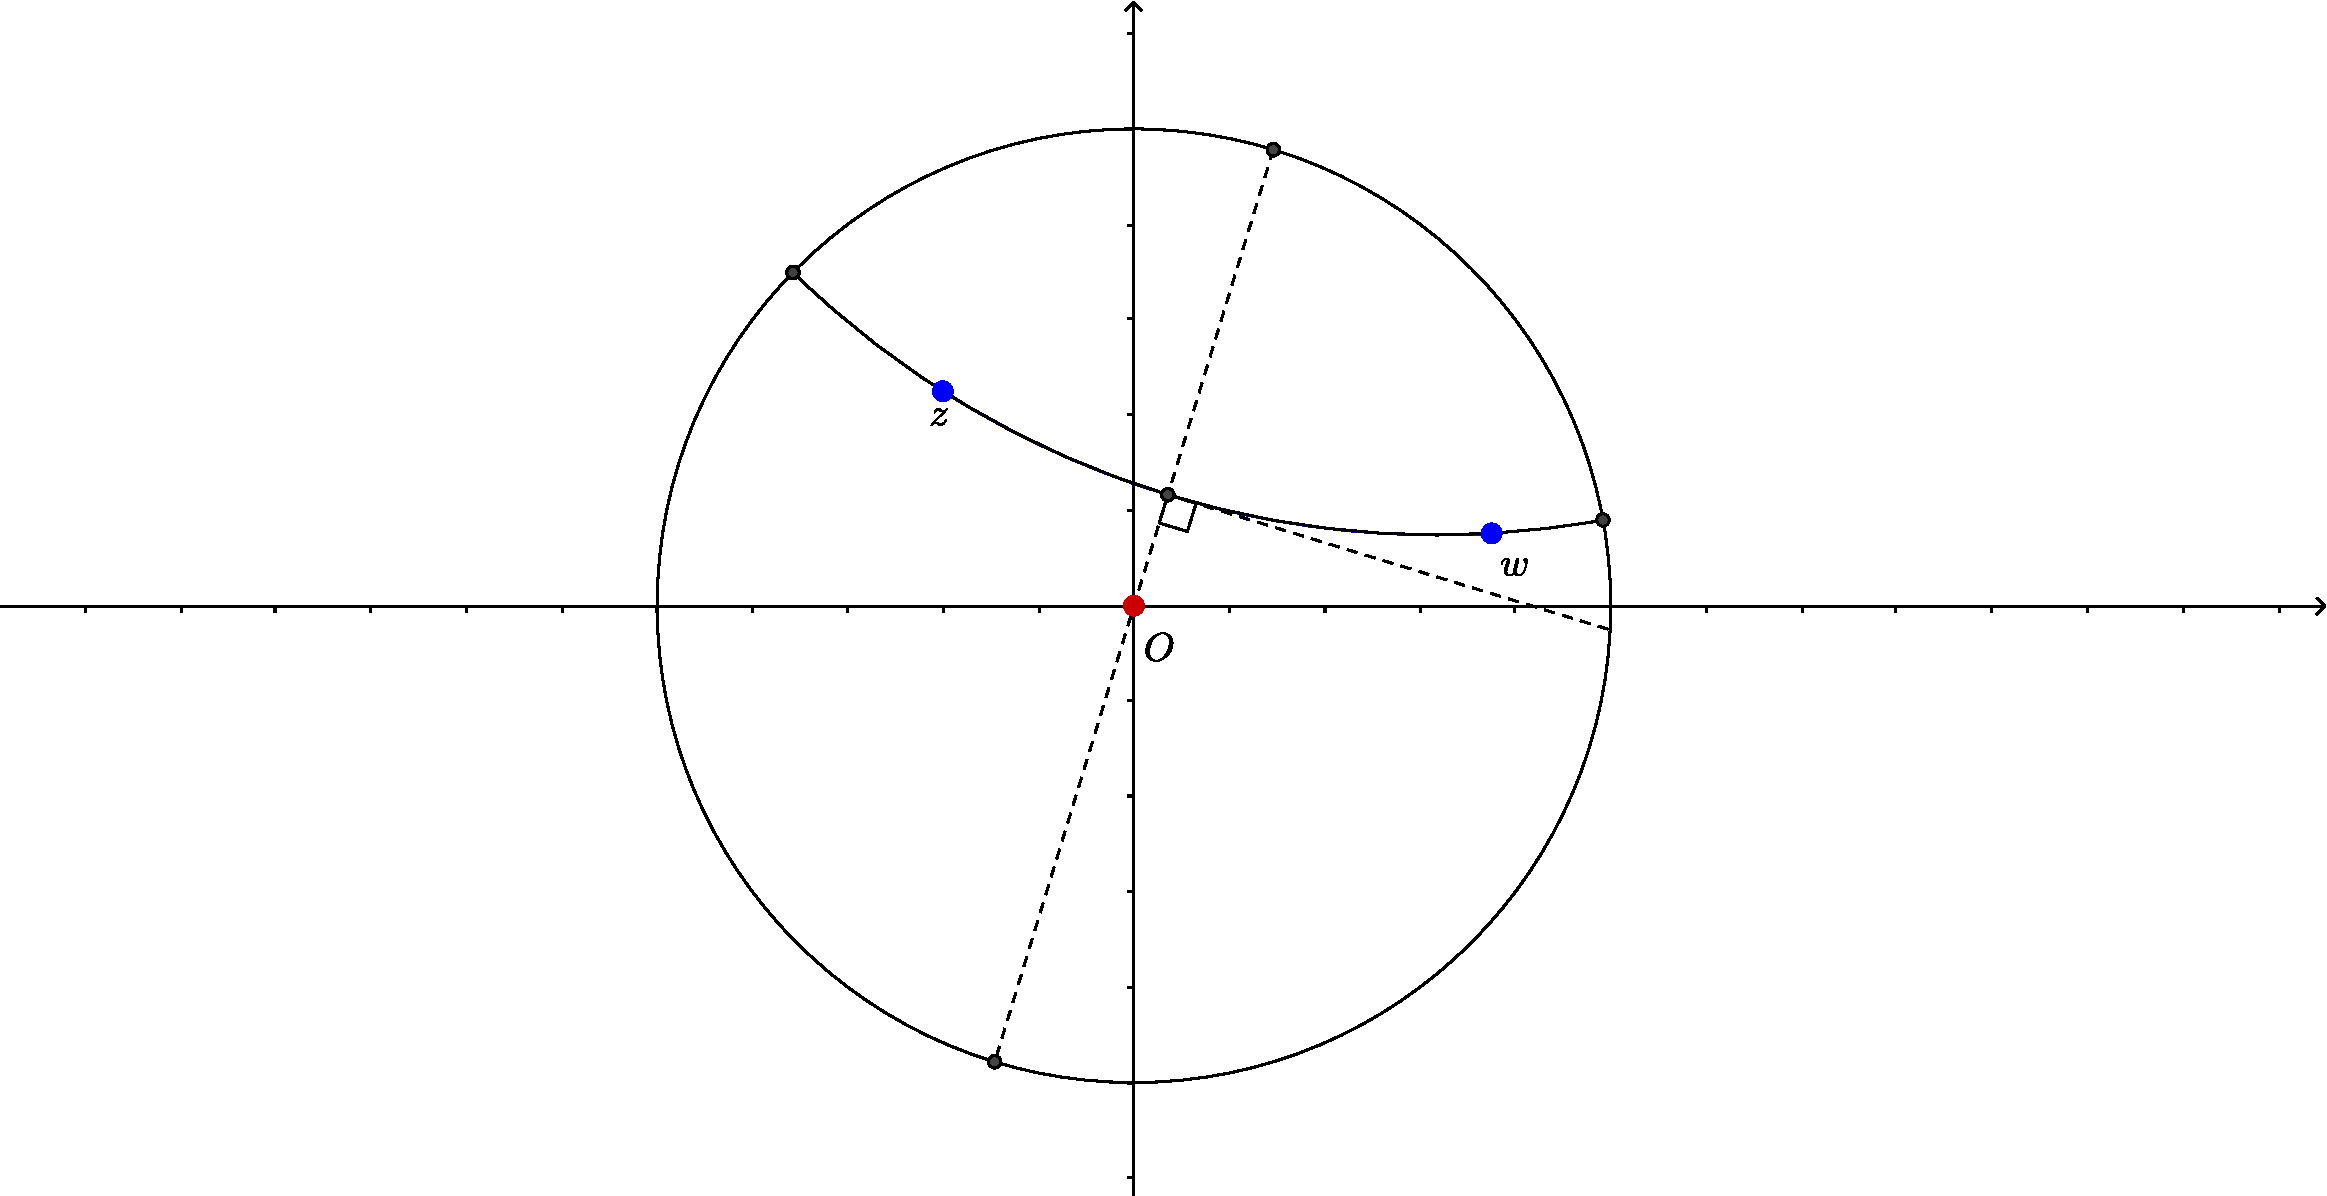
\includegraphics[width=\linewidth]{images/hyperbolic_disk_1.3.1.pdf}
        \caption{Trắc địa trong $\U$}
    \end{figure}
\end{thm}
\begin{proof}
    Nhắc lại ánh xạ phân tuyến tính $f(z)= \dfrac{iz+1}{z+i}$ là một vi phôi từ $\hh$ vào $\U$ nên nó biến biên $\partial(\hh)$ của $\hh$ thành biên $\partial(\U)$ và biến đường tròn cũng như đường thẳng trong $\C$ thành đường tròn và đường thẳng trong $\C$. Vì đường trắc địa trong $\hh$ là các nửa đường tròn hoặc đường thẳng vuông góc với trục thực (tức biên $\partial(\hh)$). Vì vậy nếu chỉ ra được $f$ là ánh xạ bảo giác (ta sẽ chứng minh ở các phần kế tiếp) thì ta sẽ chỉ ra được đường trắc địa trong $\U$ là các đoạn của các đường tròn Euclid trực giao với đường tròn đơn vị $\Sigma$ và các đường kính của nó.
\end{proof}
Tiếp theo ta đi xác định tất cả các phép biến đổi đẳng cự trên mặt phẳng hyperbolic.

Cho $PS^*L(2,\R) = S^*L(2,\R)/\{\pm I_2\}$ với $S^*L(2,\R) = \{A \in GL_2(\R)~|~\det(A) \in \{\pm 1\}\}$. Khi đó $\PSL(2,\R)$ là một nhóm con chỉ số 2 của $PS^*L(2,\R)$. Định lý sau xác định toàn bộ các phép biến đổi đẳng cự trên $\hh$.
\begin{thm}\label{thm 2.3.7}
    Nhóm các phép biến đổi đẳng cự $\Isom(\hh)$ được sinh bởi $\PSL(2,\R)$ và phép biến đổi $z\mapsto -\overline{z}$. Hơn nữa $\Isom(\hh) \cong PS^*L(2,\R)$.
\end{thm}
\begin{proof}
    Ta lần lượt có các khẳng định sau
    \begin{itemize}
        \item[i.] Với mỗi phép biến đổi đẳng cự $\varphi \in \Isom(\hh)$ thì $\varphi$ biến một đường trắc địa thành một đường trắc địa trong $\hh$.
        \item[ii.] Phép biến đổi $z\mapsto -\overline{z}$ cũng là một đẳng cự trong $\hh$.
    \end{itemize}
    Thật vậy, với mọi $z, w \in \hh$, khi đó với mọi $\xi \in [z,w]$ thì $\rho(z,w)= \rho(z,\xi)+\rho(\xi,w)$. Mà $\varphi$ là một phép biến đổi đẳng cự nên $\rho(\varphi(x),\varphi(y))=\rho(x,y)~\forall x,y\in \hh$. Dẫn đến $\rho(\varphi(z),\varphi(w)) = \rho(\varphi(z),\varphi(\xi)) + \rho(\varphi(\xi),\varphi(w))$, điều này tương đương với \[\varphi(\xi) \in [\varphi(z),\varphi(w)].\] Chứng tỏ $\varphi$ biến một đường trắc địa thành một đường trắc địa trong $\hh$. Do đó nếu kí hiệu $h-line(0,\infty)$ là trục ảo của $\hh$ thì $\varphi(h-line(0,\infty))$ là một đường trắc địa trong $\hh$. Mà tồn tại phép biến đổi $f \in \PSL(2,\R)$ biến đường trắc địa $\varphi(h-line(0,\infty))$ thành trục ảo $h-line(0,\infty)$, tức $(f\circ \varphi)(h-line(0,\infty)) = f(\varphi(h-line(0,\infty))) = h-line(0,\infty)$. 
    % Mặt khác vì $\PSL(2,\R) \subset \Isom(\hh)$ nên $f$ cũng là một đẳng cự trong $\hh$, dẫn đến $f\circ \varphi$ cũng vậy.
    % Từ đó suy ra với mọi đường trắc địa bất kỳ trong $\hh$, vì luôn tồn tại một phép biến đổi phân tuyến tính trong $\PSL(2,\R)$ biến nó thành $h-line(0,\infty)$, hợp của phép biến đổi đó với $f \circ \varphi$ cũng là một phép biến đổi đẳng cự trong $\hh$ và lại đưa về trường hợp đang xét ở trên.
    Bây giờ, với bất kì $z = x+iy \in \hh$, đặt $(f\circ \varphi)(z) = a+ib$. Khi đó với $ic \in h-line(0,\infty)$, ta có thể giả sử $f\circ \varphi$ giữ bất động trục ảo $h-line(0,\infty)$, tức $(f\circ \varphi)(ic) = ic \in h-line(0,\infty)$. Ta có
    \begin{align*}
        \rho(z,ic)
        = \rho((f\circ \varphi)(x+iy),(f\circ \varphi)(ic))
        = \rho(a+ib,ic)
    \end{align*}
    tương đương với 
    \begin{align*}
        \ln{\dfrac{|(x+iy)-\overline{ic}|+|(x+iy)-ic|}{|(x+iy)-\overline{ic}|-|(x+iy)-ic|}} &= \ln{\dfrac{|(a+ib)-\overline{ic}|+|(a+ib)-ic|}{|(a+ib)-\overline{ic}|-|(a+ib)-ic|}}\\
        % \dfrac{\dfrac{|(x+iy)-\overline{ic}|}{|(x+iy)-ic|}+1}{\dfrac{|(x+iy)-\overline{ic}|}{|(x+iy)-ic|}-1} &= \dfrac{\dfrac{|(a+ib)-\overline{ic}|}{|(a+ib)-ic|}+1}{\dfrac{|(a+ib)-\overline{ic}|}{|(a+ib)-ic|}-1}\\
        \dfrac{|(x+iy)-\overline{ic}|}{|(x+iy)-ic|} &= \dfrac{|(a+ib)-\overline{ic}|}{|(a+ib)-ic|}\\
        % ~(\text{vì hàm } h(t) = \dfrac{t+1}{t-1} \text{ đơn điệu})\\
        \dfrac{x^2+(y+c)^2}{x^2+(y-c)^2} &= \dfrac{a^2+(b+c)^2}{a^2+(b-c)^2}\\
        y(a^2 + b^2 + c^2) &= b(x^2+y^2+c^2)
    \end{align*}
    Đẳng thức trên đúng với mọi $c>0$ nên $b=y, a^2 = x^2$, tức $a+ib = x+iy$ hoặc $a+ib = -x+iy$. Nghĩa là $(f\circ \varphi)(z) = z$ hoặc $(f\circ \varphi)(z) = -\overline{z}$. Vì vậy hoặc $\varphi(z) = f^{-1}(z)$ thì $\varphi \in \PSL(2,\R)$, hoặc $\varphi(z) = f^{-1}(-\overline{z})$. Đặt $f(z) = \dfrac{\alpha z+\beta}{\gamma z+ \theta} \in \PSL(2,\R)$, khi đó $\varphi(z) = \dfrac{\alpha (-\overline{z})+\beta}{\gamma (-\overline{z})+ \theta} = \dfrac{-\alpha (\overline{z})+\beta}{-\gamma (\overline{z})+ \theta}$ với $(-\alpha) \theta - (-\gamma)\beta = -(\alpha \theta - \gamma \beta) = -1$, dẫn đến $\varphi \in PS^*L(2,\R)$. Rõ ràng $\Isom(\hh)$ được sinh bởi $\PSL(2,\R)$ và phép biến đổi $z\mapsto -\overline{z}$ và $\Isom(\hh) \cong PS^*L(2,\R)$.
\end{proof}

\subsection{Phép biến đổi bảo giác}
% Trên $\hh$ ta trang bị tích vô hướng được cảm sinh bởi tích vô hướng trên không gian tiếp xúc của $\hh$ tại $z$ là $T_z\hh \cong \C$,
% \[ \left<z_1,z_2\right> = \left<x_1+iy_1,x_2+iy_2\right>= \dfrac{1}{(\im z)^2} (x_1x_2+y_1y_2).\]
% Từ đó ta thu được chuẩn tương ứng 
% \[\norm{z_1} = \sqrt{\left<z_1,z_1\right>} = \dfrac{1}{\im z}\sqrt{x_1^2+y_1^2}\]
% và góc giữa hai vector tiếp xúc $z_1,z_2$ là góc thuộc $ [0,\pi]$ thoả mãn
%     \[ \cos\widehat{(z_1,z_2)}= \dfrac{\left<z_1,z_2\right>}{\norm{z_1}\cdot \norm{z_2}} = \dfrac{x_1x_2+y_1y_2}{\sqrt{x_1^2+y_1^2}\sqrt{x_2^2+y_2^2}}.\]
\begin{defn}[Góc giữa hai đường trắc địa] 
    Góc giữa hai đường trắc địa trong $\hh$ tại giao điểm $z$ là góc giữa hai vector tiếp xúc của chúng tại $z$ trong $T_z\hh$.
\end{defn}
\begin{defn}[Phép biến đổi bảo giác]
    Một phép biến đổi $f$ trên $\hh$ được gọi là \textit{bảo giác} nếu 
    \[\cos\widehat{(f(z_1),f(z_2))} = \cos\widehat{(z_1,z_2)},\]
    ngược lại $f$ được gọi là \textit{phản bảo giác nếu}
    \[\cos\widehat{(f(z_1),f(z_2))} = -\cos\widehat{(z_1,z_2)},\]
\end{defn}
\begin{thm}\label{thm 2.3.10}
    Mọi phép biến đổi trên $\PSL(2,\R)$ là bảo giác 
    % và phép biến đổi $z \mapsto -\overline{z}$ là phản bảo giác.
\end{thm}
\begin{proof}
    Giả sử $f \in \PSL(2,\R)$, khi đó với $z \in \hh$, gọi $\gamma_1, \gamma_2: [0,1] \to \hh$ lần lượt là hai đường cong giao nhau tại $z=\gamma_1(0)= \gamma_2(0)$ và có các vector tiếp tuyến tại $z$ lần lượt là $z-= \gamma_1'(0), z_2 =\gamma_2'(0)$. Suy ra $f\circ \gamma_1, f\circ \gamma_2$ lần lượt là các đường cong giao nhau tại $f(z)$ và có các vector tiếp xúc tại $f(z)$ là $Df(z)z_1,Df(z)z_2$ với $Df(z)$ là ma trận Jacobi của $f$ tại $z=x+iy \in \hh$. 
    
    Với $f(z) := f(x+iy) = u(x,y) + iv(x,y)$, vì $\hh \subset \C$ nên ta có thể coi $f: \R^2 \to \R^2$. Ta có 
    \[Df(z) = \begin{pmatrix}
                \dfrac{\partial u}{\partial x} & \dfrac{\partial u}{\partial y} \\
                 \dfrac{\partial v}{\partial x}& \dfrac{\partial v}{\partial y}
            \end{pmatrix}.\]
    Khi đó ta cần chỉ ra 
    \begin{align*}
         \cos\widehat{(Df(z)z_1,Df(z)z_2)} &= \cos\widehat{(z_1,z_2)}\\
         \dfrac{\left<Df(z)z_1,Df(z)z_2\right>}{\norm{Df(z)z_1}\cdot \norm{Df(z)z_2}} &= \dfrac{\left<z_1,z_2\right>}{\norm{z_1}\cdot \norm{z_2}}.
    \end{align*}
    Trong đó \[\left<Df(z)z_1,Df(z)z_2\right> = \dfrac{1}{\im f(z)} \left<z_1,(Df(z))^tDf(z)(z_2)\right>.\]
    Với 
    \[(Df(z))^tDf(z) = \begin{pmatrix}
                \dfrac{\partial u}{\partial x} & \dfrac{\partial v}{\partial x} \\
                 \dfrac{\partial u}{\partial y}& \dfrac{\partial v}{\partial y}
            \end{pmatrix} \begin{pmatrix}
                \dfrac{\partial u}{\partial x} & \dfrac{\partial u}{\partial y} \\
                 \dfrac{\partial v}{\partial x}& \dfrac{\partial v}{\partial y}
            \end{pmatrix}\]        
    Mà $f$ là ánh xạ khả vi phức (theo biến $z$) nên ta có $\dfrac{\partial u}{\partial x} = \dfrac{\partial v}{\partial y} \text{ và } \dfrac{\partial u}{\partial y} = -\dfrac{\partial v}{\partial x}$. Nên 
    \[(Df(z))^tDf(z) = \begin{pmatrix}
                \left(\dfrac{\partial u}{\partial x}\right)^2  + \left(\dfrac{\partial u}{\partial y}\right)^2 & 0 \\
                 0& \left(\dfrac{\partial u}{\partial x}\right)^2  + \left(\dfrac{\partial u}{\partial y}\right)^2
            \end{pmatrix}
            = \left[\left(\dfrac{\partial u}{\partial x}\right)^2  + \left(\dfrac{\partial u}{\partial y}\right)^2\right]\cdot I_2.
    \]
    Nên \[\left<Df(z)z_1,Df(z)z_2\right> =  \left[\left(\dfrac{\partial u}{\partial x}\right)^2  + \left(\dfrac{\partial u}{\partial y}\right)^2\right]\dfrac{1}{\im f(z)} \left<z_1,z_2\right> \]
    Tương tự thì 
    \[\norm{Df(z)z_i}^2 = \left<Df(z)z_i,Df(z)z_i\right> =  \left[\left(\dfrac{\partial u}{\partial x}\right)^2  + \left(\dfrac{\partial u}{\partial y}\right)^2\right]\dfrac{1}{\im f(z)} \left<z_i,z_i\right>, i =1,2. \]
    Từ đó ta có $f$ là một ánh xạ bảo giác.
    
    % Tiếp theo xét ánh xạ $g: z = x+iy \mapsto -\overline{z} = -x+iy$, khi đó vì $\partial g /\partial \overline{z} = -1 \neq 0$ nên $g$ không phải là hàm khả vi phức nên ta không thể làm như cách trên.
\end{proof}
% \begin{thm}
%     Topo trên $\hh$ cảm sinh bởi metric hyperbolic  giống với metric cảm sinh bởi metric Euclid.
% \end{thm}

\section{Diện tích hyperbolic và công thức Gauss-Bonnet}
Nhắc lại rằng diện tích của một tập con $A$ trong mặt phẳng Euclid $\R^2$ là 
\[\mu_{\R^2}(A) = \int_Adxdy.\]
Một cách tương tự, ta định nghĩa diện tích hyperbolic của một tập con $A$ trong mặt phẳng hyperbolic $\hh$. Tại mỗi $z\in \hh$, xét không gian vector tiếp xúc $T_z\hh$ trang bị tích vô hướng hyperbolic. Diện tích của hình bình hành sinh ra từ cơ sở chính tắc $e_1 = \begin{pmatrix}
    1\\0
\end{pmatrix},e_2 = \begin{pmatrix}
    0\\1
\end{pmatrix}$ là 
\[Vol_{hyp}(e_1,e_2) = \sqrt{\det\begin{pmatrix}
    \left<e_1,e_1\right>_{hyp} & \left<e_1,e_2\right>_{hyp}\\
    \left<e_2,e_1\right>_{hyp} & \left<e_2,e_2\right>_{hyp}
\end{pmatrix}} = \dfrac{1}{\im^2(z)}.\]
Điều này dẫn ta đến định nghĩa sau đây.
\begin{defn}
Diện tích hyperbolic của một tập con $A$ trong mặt phẳng hyperbolic $\hh$ là
\[\mu(A) = \mu_{\hh}(A) = \int_A\dfrac{dxdy}{y^2}\] 
nếu tích phân trên tồn tại.
\end{defn}

\begin{thm}
    Các phép đẳng cự thuộc $\PSL(2,\R)$ của $\hh$ bảo toàn diện tích hyperbolic. Cụ thể hơn, với mọi tập con $A \subset \hh$ và $f \in \PSL(2.\R)$ của $\hh$, ta có $\mu(f(A)) = \mu(A)$.
\end{thm}

\begin{proof}
    Giả sử $A \subset \hh$ và $\mu(A)$ tồn tại. 
    
    Lấy bất kỳ $f(z) = \dfrac{az+b}{cz+d} $ trong $\PSL(2,\R)$. Giả sử $f(z) = u(x,y)+iv(x,y)$. 
    
    Ta có
    \begin{align*}
        \mu(f(A)) = \int_{f(A)}\dfrac{dudv}{v^2}= \int_A{\dfrac{1}{v^2} |\det(Df(z))|dxdy}.
    \end{align*}
     Vì $f$ là hàm khả vi phức nên $\dfrac{\partial u}{\partial x} = \dfrac{\partial v}{\partial y} \text{ và } \dfrac{\partial u}{\partial y} = -\dfrac{\partial v}{\partial x}$. Suy ra 
     \[\left|\det(Df(z)\right| = \left|\det \begin{pmatrix}
                \dfrac{\partial u}{\partial x} & \dfrac{\partial u}{\partial y} \\
                 \dfrac{\partial v}{\partial x}& \dfrac{\partial v}{\partial y}
    \end{pmatrix}\right| = \left(\dfrac{\partial v}{\partial x}\right)^2 + \left(\dfrac{\partial v}{\partial y}\right)^2.\]
    Lại có $v = \im f(z) = \dfrac{\im z}{|cz+d|^2} = \dfrac{y}{(cx+d)^2 + c^2y^2}$ nên 
    \[\left(\dfrac{\partial v}{\partial x}\right)^2 + \left(\dfrac{\partial v}{\partial y}\right)^2 = \left(\dfrac{1}{(cx+d)^2 + c^2y^2}\right)^2.\]
    Từ đó ta được 
    \begin{align*}
        \mu(f(A)) 
        &= \int_A{\left(\dfrac{(cx+d)^2 + c^2y^2}{y}\right)^2 \left(\dfrac{1}{(cx+d)^2 + c^2y^2}\right)^2dxdy}
        = \int_A\dfrac{dxdy}{y^2} = \mu(A).
    \end{align*}
\end{proof}
\begin{defn}[Đa giác hyperbolic]
    Một đa giác hyperbolic $n-$cạnh trong $\hh$ là một tập con đóng của $\overline{\hh} = \hh \cup \R \cup \{\infty\}$, bị chặn bởi các đoạn trắc địa $[z_1,z_2],\ldots,[z_n,z_1]$. Các $z_i$ là giao của hai đoạn trắc địa của đa giác được gọi là đỉnh của đa giác hyperbolic đó.
\end{defn}
% \begin{exam*}
%     Lần lượt sau đây là các tam giác số đỉnh nằm trên $\R \cup \{\infty\}$ là $0,1,2,3$.
%     \begin{figure}[htp!]
%         \centering
%         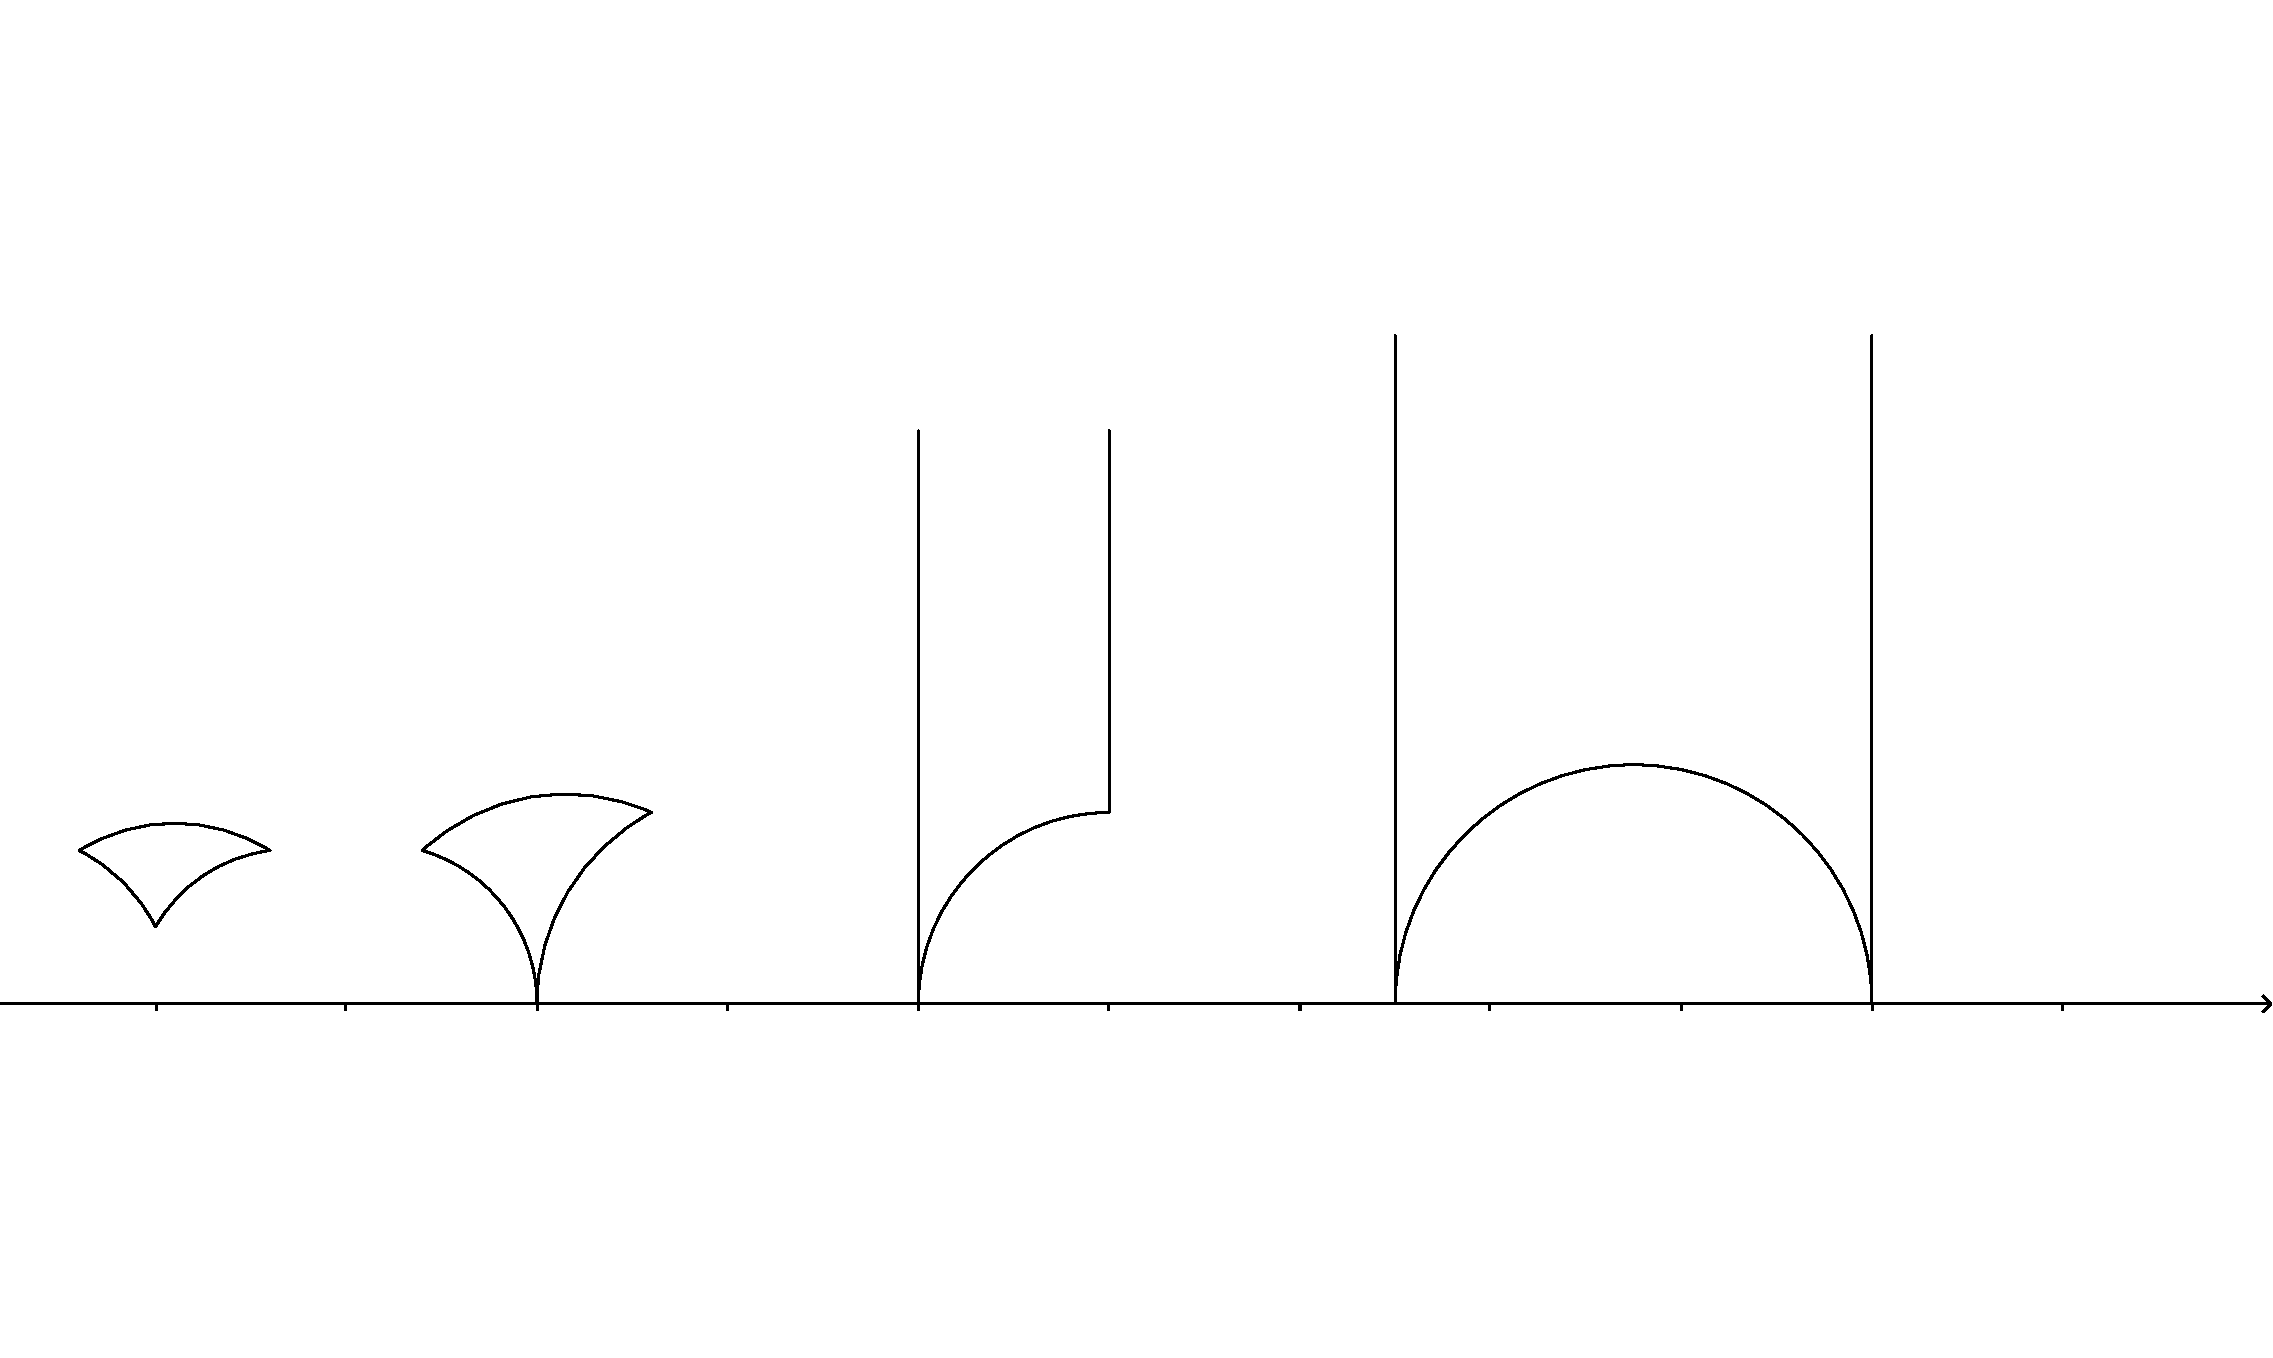
\includegraphics[width=0.7\linewidth]{images/polygon.pdf}
%         \caption{Tam giác hyperbolic}
%         \label{fig:enter-label}
%     \end{figure}
% \end{exam*}
Tiếp theo chúng ta đến với công thức Gauss-Bonnet để tính diện tích của tam giác hyperbolic.
\subsubsection{Định lý Gauss-Bonnet}
\begin{thm}[Gauss-Bonnet]\label{thm 2.4.5}
    Cho $\Delta$ là một tam giác hyperbolic với các góc $\alpha, \beta, \gamma$. Khi đó \[\mu(\Delta) = \pi - (\alpha + \beta + \gamma).\]
\end{thm}
\begin{proof}
    Giả sử $\Delta$ là một tam giác hyperbolic có các đỉnh lần lượt là $A,B,C \in \overline{\hh} = \hh \cup \R\cup \{\infty\}$ và các góc tương ứng các đỉnh lần lượt là $\alpha,\beta, \gamma$. 

    Khi đó ta có các trường hợp sau
    \begin{enumerate}
        \item $\Delta$ có một trong 3 đỉnh thuộc $\R \cup \{\infty\}$. 
        
        Không mất tính tổng quát, ta có thể giả sử $A, B \in \hh$, $C = \infty$.
        
        Vì nếu $C = r \in \R$. Xét phép biến đổi $T(z) = \dfrac{-1}{z-r}$ trong $\PSL(2,\R)$. Qua tác động của $T$ thì $T(A),T(B) \in \hh$ và $T(C) = \infty$. Mà $T$ bảo toàn diện tích hyperbolic và cũng bảo toàn góc trong $\hh$ nên \[\mu(T(A)T(B)T(C)) = \mu(\Delta).\]
        Khi đó trắc địa qua $A, \infty$ và trắc địa qua $B,\infty$ sẽ là các đường hyperbolic vuông góc với trục thực. Còn trắc địa qua $A,B$ là một nửa đường tròn vuông góc với trục thực.
        
        Bằng cách tác động một cách phù hợp các đẳng cự có dạng $z\mapsto z+k,k\in \R$ hoặc $z\mapsto \lambda z, \lambda>0$ trong $\PSL(2,\R)$, mà vẫn bảo toàn diện tích hyperbolic cũng như bảo toàn góc. Ta có thể giả sử trắc địa qua $A,C$ là $h-line(a,\infty)$, trắc địa qua $B,C$ là $h-line(b,\infty)$ và trắc địa qua $A,B$ là $h-line(-1,1)$. 

        \begin{figure}[htp!]
            \centering
            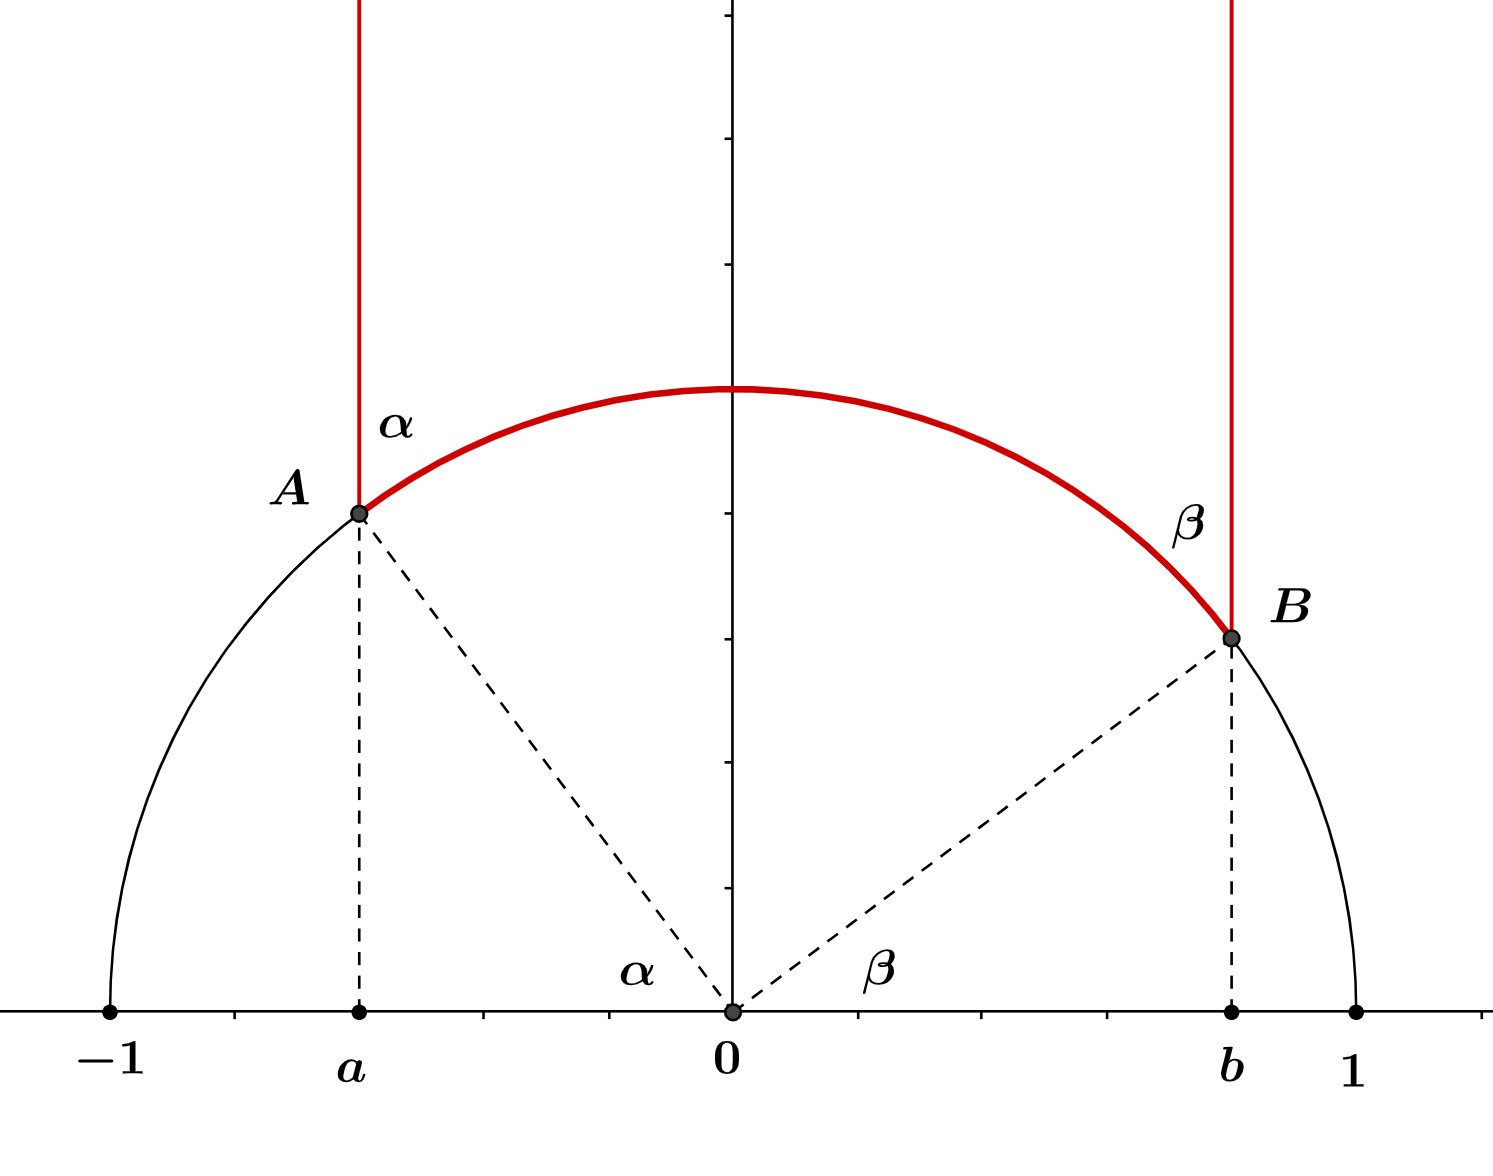
\includegraphics[width=0.4\linewidth]{images/Gauss-Bonnet_1.png}
            % \caption{}
            % \label{fig:enter-label}
        \end{figure}
        Đường cong tham số qua $A,B$ là $y = \sqrt{1-x^2}, a \leq x \leq b$. 
        Do đó \begin{align*}
            \mu(\Delta) = \int_{\Delta}{\dfrac{dxdy}{y^2}} = \int_a^b{dx}\int_{\sqrt{1-x^2}}^{\infty}{\dfrac{dy}{y^2}} = \int_a^b{\dfrac{dx}{\sqrt{1-x^2}}}.
        \end{align*}
        Đặt $x = \cos\theta$ với $\theta \in [0,\pi]$. Khi đó 
        \[\mu(\Delta) = \int_{\pi-\alpha}^{\beta}{\dfrac{-\sin\theta d\theta}{\sin\theta}} = \pi -\alpha -\beta=\pi-(\alpha + \beta + \gamma)~(\text{vì }\gamma = 0).\]

        \item $\Delta$ không có đỉnh nào trong $\R \cup \{\infty\}$.

        Ta có thể tác động các phép biến đổi trong $\PSL(2,\R)$ sao cho trắc địa qua các cạnh của $\Delta$ đều là các nửa đường tròn vuông góc với trục thực. Giả sử trắc địa qua $A,C$ cắt trục thực tại $D$. Kí hiệu $\Delta_1$ là tam giác hyperbolic có 3 đỉnh là $A,B,D$ và $\Delta_2$ là tam giác hyperbolic có 3 đỉnh là $B,C,D$, hai tam giác này đều có 1 đỉnh trên $\R\cup\{\infty\}$ và 2 đỉnh còn lại trên $\hh$. Áp dụng công thức tính diện tích của chúng như trường hợp 1 ta được
        \begin{figure}
            \centering
            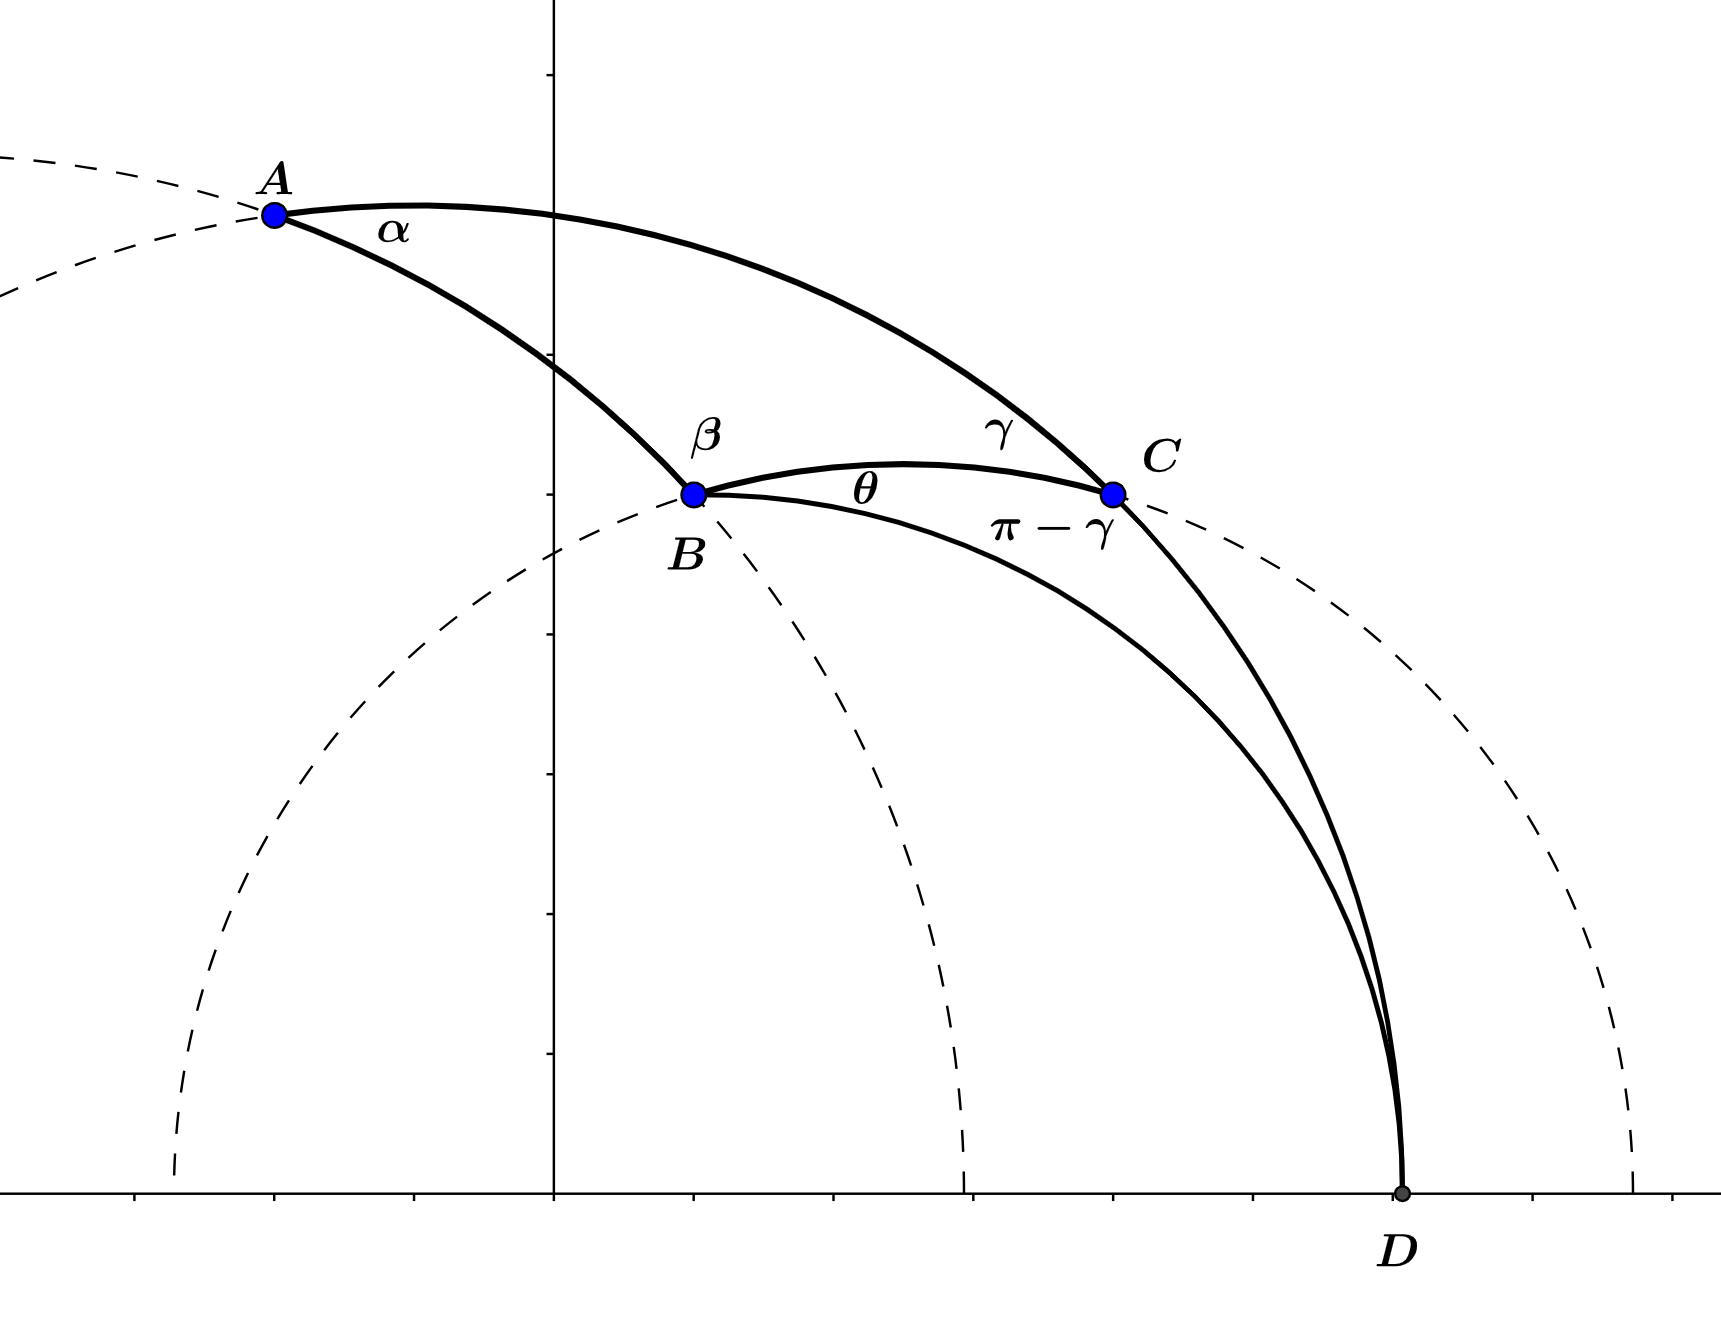
\includegraphics[width=0.4\linewidth]{images/gauss-bonnet-2.png}
            % \caption{Enter Caption}
            % \label{fig:enter-label}
        \end{figure}
        \[\mu(\Delta) = \mu(\Delta_1) -\mu(\Delta_2) = [\pi - (\alpha)-(\beta + \theta)] - [\pi - (\theta + \pi -\gamma)] = \pi -\alpha - \beta -\gamma.\]
        
        \item $\Delta$ có hai đỉnh trong $\R \cup \{\infty\}$ và đỉnh còn lại thuộc $\hh$.
    
        Giả sử $A \in \hh, B \in \R$ và $C = \infty$ (còn trường hợp $A \in \hh,~B,C \in \R$, ta có thể tác động một đẳng cự biến $B\mapsto \infty$). Khi đó $\beta =0 = \gamma$ và 
        \[\mu(ABC) = \mu(ABD) + \mu(ADC) = \pi-(\theta+\phi) + \pi -(\alpha - \theta) - (\pi-\phi) = \pi - \alpha = \pi-(\alpha + \beta + \gamma).\]

        \begin{figure}[htp!]
        \centering
        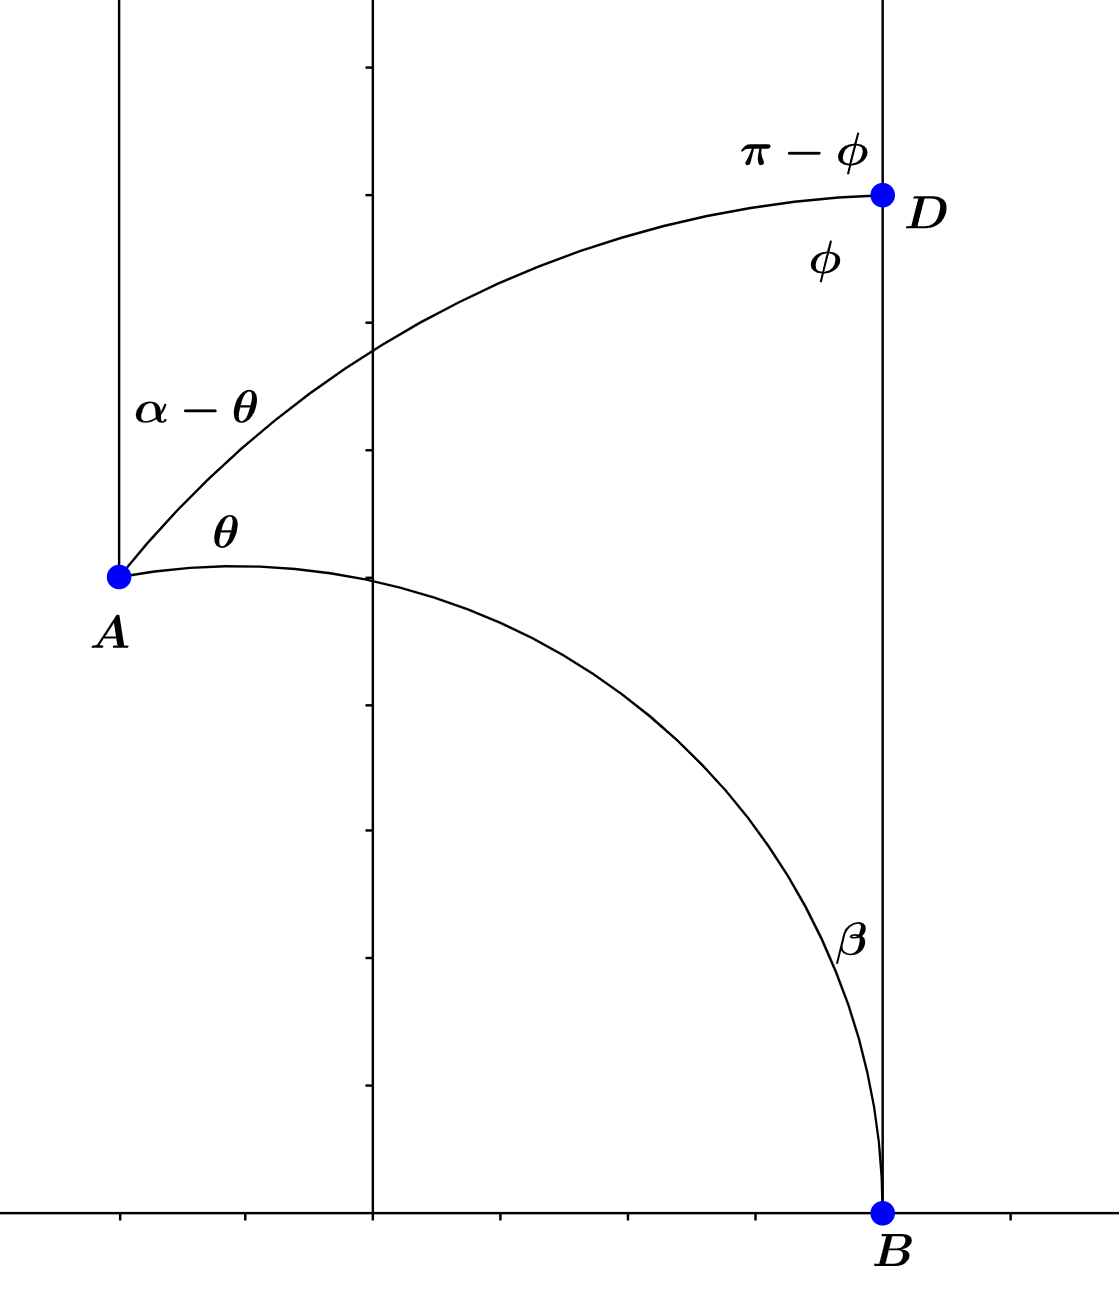
\includegraphics[width=0.3\linewidth]{images/Gauss-Bonnet_3.png}
        % \caption{Enter Caption}
        % \label{fig:enter-label}
        \end{figure}
    \item $\Delta$ có 3 đỉnh trên $\R \cup \{\infty\}$.

        Giả sử $A,B \in \R, C = \infty$ (nếu $A,B,C \in \R$, bằng đẳng cự có dạng $z \mapsto \dfrac{-1}{z-k}$ phù hợp ta có thể đưa một trong 3 đỉnh trên thành $\infty$).
        
        Khi đó, bằng tác động phép đẳng cự phù hợp có dạng $z\mapsto z+k$, ta có thể giả sử trắc địa qua $A,C$ là $h-line(-a,\infty)$, trắc địa qua $B,C$ là $h-line(a,\infty)$ và đẳng cự qua $A,B$ là $h-line(-a,a)$.
        \begin{figure}[htp!]
        \centering
        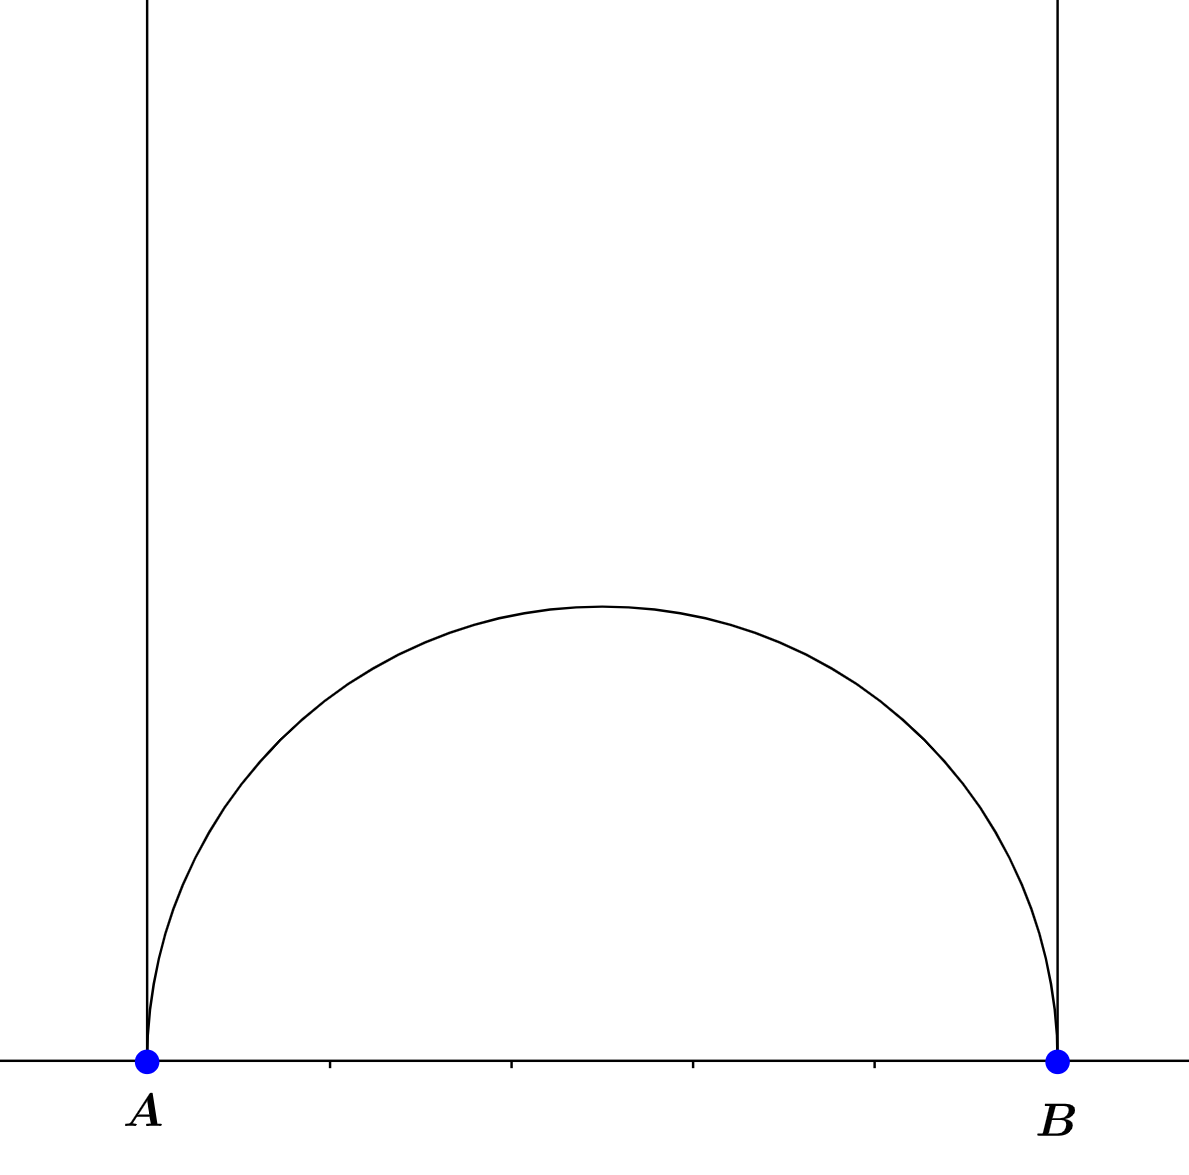
\includegraphics[width=0.3\linewidth]{images/Gauss-Bonnet_4.png}
        % \caption{Enter Caption}
        % \label{fig:enter-label}
        \end{figure}
        Do đó $\alpha = \beta =\gamma = 0$ và 
        \begin{align*}
            \mu(\Delta) = \int_{\Delta}{\dfrac{dxdy}{y^2}} = \int_{-a}^a{dx}\int_{\sqrt{a^2-x^2}}^{\infty}{\dfrac{dy}{y^2}} = \int_{-a}^a{\dfrac{dx}{\sqrt{a^2-x^2}}} = \pi = \pi -(\alpha+\beta + \gamma).
        \end{align*}
    \end{enumerate}
    Vậy ta luôn có $\mu(\Delta) = \pi -(\alpha+\beta + \gamma).$
\end{proof}

\section{Lượng giác hyperbolic}
Với mỗi số $a > 0$, ta định nghĩa góc song song tương ứng với $a$ bởi góc $\Pi(a)$ như hình tam giác hyperbolic vuông có một đỉnh ở vô cùng, cạnh hữu hạn bằng $a$.
\begin{figure}[htp!]
    \centering
    \includegraphics[width=0.5\linewidth]{images/góc song song.png}
    \caption{Góc song song}
    \label{fig:enter-label}
\end{figure}
\begin{thm}\label{thm 2.5.1}
    Cho $\Delta$ là tam giác hyperbolic với hai góc là $0, \pi/2$ và một cạnh độ dài hữu hạn $a > 0$. Khi đó góc thứ ba là $\Pi(a)$ thoả mãn
    \begin{enumerate}
        \item $\tan{\Pi(a)} = \dfrac{1}{\sinh{a}},$
        \item $\sin{\Pi(a)} = \dfrac{1}{\cosh{a}},$
        \item $\sec{\Pi(a)} = \dfrac{1}{\tanh{a}}.$
    \end{enumerate}
\end{thm}
\begin{proof}
    Giả sử 3 đỉnh tam giác hyperbolic vuông trên là $z = x+iy, w, \infty$.
    
    Tác động phép biến đổi $z \mapsto z - x$ trong $\PSL(2,\R)$ vào tam giác trên ta được $z \mapsto z'= iy, w \mapsto  w' = y\cos{\Pi(a)} + i y\sin{\Pi(a)}$. 
    Ta có 
    \begin{align*}
        \cosh{a} = \cosh{\rho(z,w)} &= \cosh{\rho(z',w')} = 1 + \dfrac{|z'-w'|^2}{2\im(z')\im(w')}\\
        &= 1 + \dfrac{(0-y\cos{\Pi(a)})^2+ (y-y\sin{\Pi(a)})^2}{2y^2\sin{\Pi(a)}}\\
        &= \dfrac{1}{\sin{\Pi(a)}}\\
    \end{align*}
    Do đó 
    $\sinh a = \sqrt{\cosh^2{a}-1} = \sqrt{\dfrac{1}{\sin^2{\Pi(a)}}-1} = \dfrac{1}{\tan{\Pi(a)}}$. \\
    Vì vậy $\tanh(a) = \dfrac{\sinh{a}}{\cosh{a}} = \cos(\Pi(a)) = \dfrac{1}{\sec{\Pi(a)}}$.
\end{proof}
Tiếp theo ta tìm hiểu về mối liên hệ giữa các góc và cạnh trong tam giác hyperbolic. Xét tam giác hyperbolic hữu hạn có độ dài 3 cạnh lần lượt là $a,b,c$ và 3 góc tương ứng đối diện là $\alpha, \beta, \gamma$. 
\begin{thm}\label{thm 2.5.2}
    \begin{itemize}
        \item [i.]Quy tắc $\sin$: $\dfrac{\sinh a}{\sin \alpha} = \dfrac{\sinh b}{\sin \beta} = \dfrac{\sinh c}{\sin \gamma}$.
        \item [ii.] Quy tắc $\cos I$: $\cosh c = \cosh a \cosh b - \sinh a \sinh b \cos{\gamma}$.
        \item[iii.] Quy tắc $\cos II$: $\cosh{c} =\dfrac{\cos \alpha \cos \beta + \cos \gamma }{\sin \alpha \sin \beta}$.
    \end{itemize}
\end{thm}
    \begin{remark*}    
    Trong mô hình đĩa Poincare thì khoảng cách giữa hai điểm $z,w \in \U$ được định nghĩa bởi 
    \[\rho^*(f(z),f(w)) = \rho(z,w),\]
    \[\rho^*(z,w) = \rho(f^{-1}(z),f^{-1}(w)), \]
    với ánh xạ phân tuyến tính chuyển từ $\hh$ lên $\U$ là
    \[f: \hh \to \U, z\mapsto \dfrac{z-i}{iz-1}\]
    và ngược lại ánh xạ ngược của nó gửi $\U$ thành $\hh$ là
    \[f^{-1}:\U \to \hh, z\mapsto \dfrac{-z+i}{-iz+1}.\]
    Ta có các công thức \[\sinh\left(\dfrac{1}{2}\rho^*(z,w)\right) = \dfrac{|z-w|^2}{(1-|z|^2)(1-|w|^2)}\] và \[\tanh{\left(\dfrac{1}{2}\rho^*(z,w)\right)} = \left|\dfrac{z-w}{1-z\overline{w}}\right|.\]
    Với mỗi $g \in \PSL(2,\R)$ thì $g$ là một đẳng cự trên $\hh$. Từ đó $f \circ g \circ f^{-1}$ là một đẳng cự trên $\U$. Ta có
    \[\begin{tikzcd}
    	\hh && \hh \\
    	\\
    	\U && \U
    	\arrow["g", from=1-1, to=1-3]
    	\arrow["f"', from=1-1, to=3-1]
    	\arrow["{f\circ g \circ f^{-1}}"', from=3-1, to=3-3]
    	\arrow["f"', shift right=3, from=1-3, to=3-3]
    	\arrow["{f^{-1}}"', shift right=2, from=3-3, to=1-3]
    \end{tikzcd}\]
    \begin{align*}
        \rho^*(f \circ g \circ f^{-1}(z),f \circ g \circ f^{-1}(w))
        &= \rho(g \circ f^{-1}(z), g \circ f^{-1}(w))\\
        &= \rho(f^{-1}(z), f^{-1}(w))\\
        &= \rho^*(z,w).
    \end{align*}
\end{remark*}
\textbf{Quay trở lại với định lí trên}
\begin{proof}
Đầu tiên ta sẽ chứng minh 
\[\cosh c = \cosh a \cosh b - \sinh a \sinh b \cos{\gamma}.\]
    \begin{figure}[htp]
        \centering
        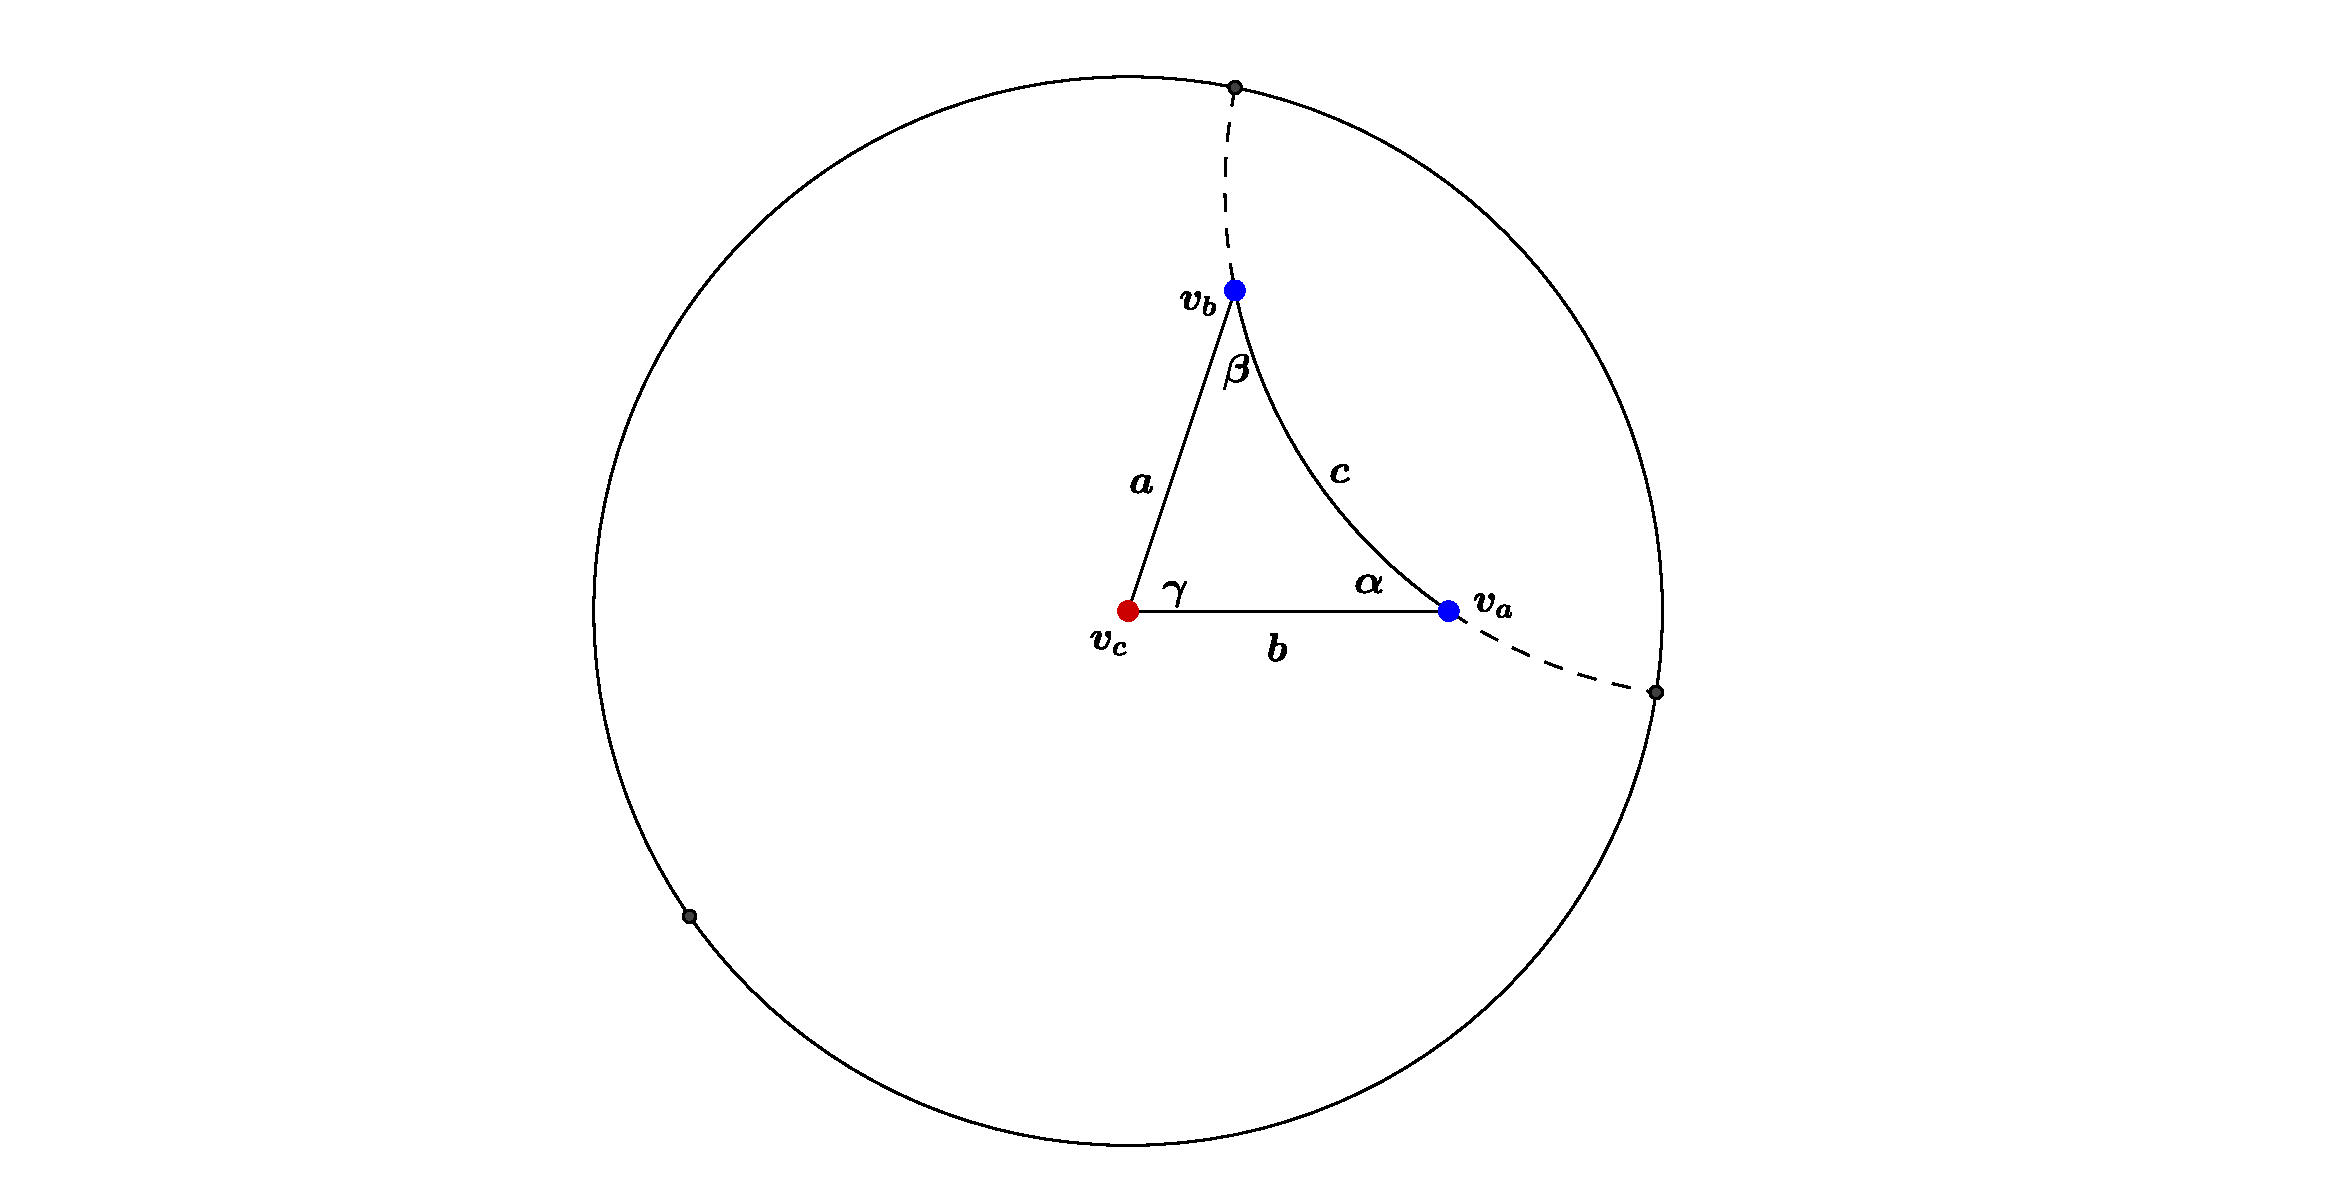
\includegraphics[width=0.8\linewidth]{images/PoincareModel.pdf}
        \caption{Đĩa Poincare $\U$}
        \label{fig:enter-label}
    \end{figure}
    Gọi các đỉnh của tam giác hyperbolic trên $\U$ lần lượt là $v_a,v_b,v_c$ với khoảng cách hyperbolic các cạnh là $a,b,c$ và các góc tương ứng $\alpha, \beta, \gamma$. Không mất tổng quát ta có thể giả sử $v_c \equiv 0, \im(v_a) = 0, \re(v_a) > 0$, khi đó 
        \[\tanh{\left(\dfrac{1}{2}\rho^*(v_a,v_c)\right)} = \left|\dfrac{v_a-0}{1-v_a\overline{0}}\right|\]
        tức $v_a = \tanh{(b/2)}$, và 
        \[\tanh{\left(\dfrac{1}{2}\rho^*(v_b,v_c)\right)} = \left|\dfrac{v_b-0}{1-v_b\overline{0}}\right|,\]
        tức $|v_b| = \tanh{(a/2)}$, dẫn đến $v_b = \tanh{(a/2)}e^{i\gamma}$.
        Từ đó suy ra
        \begin{align*}
            \cosh c &= \cosh(\rho^*(v_a,v_b)) \\
            &= 1+ 2 \sinh^2{\left(\dfrac{\rho^*(v_a,v_b)}{2}\right)}\\
            &= 1+ 2 \dfrac{|v_a -v_b|^2}{(1-|v_a|^2)(1-|v_b|^2)}\\
            &= 1+ 2 \dfrac{|\tanh{(b/2)} -\tanh{(a/2)}e^{i\gamma}|^2}{(1-\tanh^2{(b/2)})(1-\tanh^2{(a/2)})}\\
            &= 1+ 2\dfrac{|x-y(\cos{\gamma} + i \sin{\gamma})|^2}{(1-x^2)(1-y^2)} (\text{ với } x = \tanh{(b/2)}, y = \tanh{(a/2)})\\
            % &= \dfrac{(1-x^2)(1-y^2) + 2[(x-y\cos{\gamma})^2+y^2\sin^2\gamma]}{(1-x^2)(1-y^2)}\\
            &= \dfrac{x^2y^2+x^2+y^2+1}{(1-x^2)(1-y^2)}-\dfrac{4xy}{(1-x^2)(1-y^2)}\cos{\gamma}
        \end{align*}
        Mà $1-y^2 = 1 - \tanh^2{(a/2)} 
        % = 1 - \dfrac{\sinh^2(a/2)}{\cosh^2(a/2)}= \dfrac{\cosh^2(a/2)-\sinh^2(a/2)}{\cosh^2(a/2)} 
        = \dfrac{1}{\cosh^2(a/2)}$, tương tự thì 
        $1-x^2 = \dfrac{1}{\cosh^2(b/2)}$, dẫn đến 
        \begin{align*}
            &\dfrac{x^2y^2+x^2+y^2+1}{(1-x^2)(1-y^2)}\\
            &= (\tanh^2(a/2)\tanh^2(b/2) + \tanh^2(a/2) + \tanh^2(b/2) +1)\cosh^2(a/2)\cosh^2(b/2)\\
            &= \cosh^2(a/2)\cosh^2(b/2) + \sinh^2(a/2)\sinh^2(b/2) + \sinh^2(a/2)\cosh^2(b/2) + \sinh^2(b/2)\cosh^2(a/2)\\
            &= [\cosh(a/2)\cosh(b/2)+\sinh(a/2)\sinh(b/2)]^2+[\sinh(a/2)\cosh(b/2)-\sinh(b/2)\cosh(a/2)]^2\\
            &= \cosh^2\dfrac{a+b}{2} + \sinh^2\dfrac{a-b}{2}
            = \dfrac{[\cosh(a+b)+1]+[\cosh(a-b) -1]}{2}
            = \cosh a\cosh b,
        \end{align*}
        và 
        \begin{align*}
            \dfrac{4xy}{(1-x^2)(1-y^2)}
            &= 4\tanh(1/2)\tanh(b/2)\cosh^2(a/2)\cosh^2(b/2)
            % &= 4\sinh(a/2)\cosh(a/2)\sinh(b/2)\cosh(b/2)\\
            = \sinh a\sinh b.
        \end{align*}
        Vì vậy ta thu được $\cosh c = \cosh a \cosh b - \sinh a \sinh b \cos{\gamma}$.
        
        Tiếp theo ta chứng minh quy tắc $\sin$: 
        \[\dfrac{\sinh a}{\sin \alpha} = \dfrac{\sinh b}{\sin \beta} = \dfrac{\sinh c}{\sin \gamma}.\]
        Ta có 
        \begin{align*}
            \left(\dfrac{\sin{\gamma}}{\sinh c}\right)^2 
            &= \dfrac{1-\cos^2\gamma}{\sinh^2(c)}\\
            &= \dfrac{1-\left(\dfrac{\cosh a\cosh b-\cosh c}{\sinh a\sinh b}\right)^2}{\sinh^2(c)}\\
            % &= \dfrac{(\sinh a\sinh b-\cosh a\cosh b+\cosh c)(\sinh a\sinh b+\cosh a\cosh b-\cosh c)}{\sinh^2 a \sinh^2 b\sinh^2 c}\\
            % &= \dfrac{(\sinh a\sinh b-\cosh a\cosh b+\cosh c)(\sinh a\sinh b+\cosh a\cosh b-\cosh c)}{\sinh^2 a \sinh^2 b\sinh^2 c}\\
            &= \dfrac{(\cosh c-\cosh(a-b))(\cosh(a+b)-\cosh c)}{\sinh^2 a \sinh^2 b\sinh^2 c}\\
            &= \dfrac{4\sinh\dfrac{b+c-a}{2}\sinh\dfrac{c+a-b}{2}\sinh\dfrac{a+b-c}{2}\sinh\dfrac{a+b+c}{2}}{\sinh^2 a \sinh^2 b\sinh^2 c}.\\
        \end{align*}
        là một biểu thức đối xứng của $a,b,c$, tương tự cho $\dfrac{\sin \alpha}{\sinh a} \text{ và } \dfrac{\sin \beta}{\sinh b}$ ta thu được điều cần chứng minh.

        Cuối cùng ta chứng minh quy tắc $\cos II$: 
        \[\cosh{c} =\dfrac{\cos \alpha \cos \beta + \cos \gamma }{\sin \alpha \sin \beta}.\]
        Đặt $A = \cosh a, B = \cosh b, C = \cosh c$ thì
        \begin{align*}
            &\sinh a = \sqrt{A^2-1},\quad \sinh b = \sqrt{B^2-1},\quad \sinh c = \sqrt{C^2-1},\\
            &\cos \alpha = \dfrac{BC-A}{\sqrt{B^2-1}\sqrt{C^2-1}}, \quad
            \cos \beta = \dfrac{AC-B}{\sqrt{A^2-1}\sqrt{C^2-1}}, \quad 
            \cos \gamma = \dfrac{AB-C}{\sqrt{A^2-1}\sqrt{B^2-1}},\\
            &\sin \alpha = \sqrt{\dfrac{-A^2-B^2-C^2+2ABC+1}{(B^2-1)(C^2-1)}}, \quad
            \sin \beta = \sqrt{\dfrac{-A^2-B^2-C^2+2ABC+1}{(A^2-1)(C^2-1)}}.
        \end{align*}
        Suy ra 
        \begin{align*}
            \dfrac{\cos \alpha \cos \beta + \cos \gamma }{\sin \alpha \sin \beta}
            % &= \dfrac{\dfrac{BC-A}{\sqrt{B^2-1}\sqrt{C^2-1}}\dfrac{AC-B}{\sqrt{A^2-1}\sqrt{C^2-1}} + \dfrac{AB-C}{\sqrt{A^2-1}\sqrt{B^2-1}}}{\sqrt{\dfrac{-A^2-B^2-C^2+2ABC+1}{(B^2-1)(C^2-1)}}\sqrt{\dfrac{-A^2-B^2-C^2+2ABC+1}{(A^2-1)(C^2-1)}}}\\
            &= C = \cosh c.
        \end{align*}
        Kết thúc chứng minh.
\end{proof}
\begin{cor}[Định lý Pythagoras]
    Nếu $\gamma = \pi /2$ thì $\cosh c = \cosh a\cosh b$.
\end{cor}
% \section{Bài tập chương 1}
\begin{ex}
    Cho $L$ là một đường tròn Euclid hoặc một đường thẳng vuông góc với trục thực sao cho $L$ giao với trục thực tại một điểm hữu hạn $\alpha$ nào đó. Chứng minh phép biến đổi $T(z)=-(z-\alpha)^{-1}+\beta \in \PSL(2,\R)$, và với $\beta$ phù hợp thì $L$ được biến thành trục ảo.
\end{ex}
\begin{sol*}
Ta có $T$ là hợp thành của hai phép biến đổi phân tuyến tính trong $\PSL(2,\R)$ là $f(z) = \dfrac{0z-1}{z-\alpha} = \dfrac{-1}{z-\alpha},~g(z) = \dfrac{z+\beta}{0z+1}=z+\beta$ \big(nói rõ hơn $z\xlongrightarrow[]{f}\dfrac{-1}{z-\alpha}\xlongrightarrow[]{g}\dfrac{-1}{z-\alpha} + \beta$\big). Vì $\PSL(2,\R)$ là một nhóm với phép toán là phép hợp thành ánh xạ nên với $f,g\in \PSL(2,\R)$ thì $T = g\circ f \in \PSL(2,\R)$.
\begin{itemize}
    \item Nếu $L$ là đường thẳng Euclid vuông góc với trục thực thì 
    \[L = \{z\in \C~|~\re(z) = \alpha\} = \{\alpha + iy ~|~y \in \R\}.\] 
    Với $y\neq 0,~T(\alpha + iy) = \dfrac{-1}{(\alpha + iy)-\alpha} + \beta = i\dfrac{1}{y} + \beta$, còn khi $y=0$ thì $T(\alpha) \to \infty$. Do đó để $T(\alpha + iy)$ thuộc trục ảo thì $\beta = 0$ (do $\beta \in \R$).
    \item Nếu $L$ là đường tròn Euclid vuông góc với trục thực thì nó còn giao với trục thực tại điểm $\gamma$ nào đó khác $\alpha$. Hơn nữa, tâm của $L$ là trung điểm $c = \dfrac{\alpha + \gamma}{2}$ của đoạn thẳng nối $\alpha$ và $\gamma$ trên trục thực, bán kính của $L$ là $r = |\alpha - c| = \bigg|\dfrac{\alpha-\gamma}{2}\bigg|$. Nghĩa là \[L = \{z\in \C~|~|z-c| = r\} = \big\{c+re^{i\theta}~|~\theta \in [0, 2\pi]\big\}.\]
    Suy ra $\forall \theta \in [0,2\pi]$ thì 
    \begin{align*}
        T(c+re^{i\theta}) &= -\dfrac{1}{(c+re^{i\theta})-\alpha} + \beta\\
        & = -\dfrac{1}{(c-\alpha+r\cos{\theta}) + ir\sin{\theta}} + \beta\\
        & = -\dfrac{((c-\alpha+r\cos{\theta}) - ir\sin{\theta})}{(c-\alpha+r\cos{\theta})^2 + (r\sin{\theta})^2} + \beta\\
        &= \left(\beta - \dfrac{c-\alpha+r\cos{\theta}}{(c-\alpha+r\cos{\theta})^2 + (r\sin{\theta})^2}\right) + i\dfrac{r\sin{\theta}}{(c-\alpha+r\cos{\theta})^2 + (r\sin{\theta})^2}
    \end{align*}
    Do đó để $T(c+re^{i\theta})$ thuộc trục ảo thì $\beta - \dfrac{c-\alpha+r\cos{\theta}}{(c-\alpha+r\cos{\theta})^2 + (r\sin{\theta})^2} = 0~\forall \theta \in [0,2\pi]$. Nghĩa là 
    \begin{align*}
        \beta & = \dfrac{c-\alpha+r\cos{\theta}}{(c-\alpha+r\cos{\theta})^2 + (r\sin{\theta})^2}\\
        &= \dfrac{c-\alpha+r\cos{\theta}}{(c-\alpha)^2+2r(c-\alpha)\cos{\theta} + r^2}\\
        &= \dfrac{c-\alpha+r\cos{\theta}}{2(c-\alpha)^2+2r(c-\alpha)\cos{\theta}}~(\text{do } r^2 = |\alpha-c|^2 = (\alpha-c)^2)\\
        &= \dfrac{1}{2(c-\alpha)} = \dfrac{1}{\gamma -\alpha}~\left(\text{do }c =\dfrac{\alpha + \gamma}{2} \right).
    \end{align*}
\end{itemize}
\end{sol*}
\begin{ex}
    Chứng minh với $z \in \hh$ và $f(z) = \dfrac{zi+1}{z+i}$ thì $\dfrac{2|f'(z)|}{1-|f(z)|^2}=\dfrac{1}{\im(z)}\cdot$
\end{ex}
\begin{sol*}
Ta có $f'(z) = \dfrac{-2}{(z+i)^2}$ nên 
\[|f'(z)| = \left|\dfrac{-2}{(z+i)^2}\right| = \dfrac{2}{|z+i|^2} = \dfrac{2}{(z+i)(\overline{z}-i)}=\dfrac{2}{z\overline{z}+i(z-\overline{z})+1}=\dfrac{2}{|z|^2+2\im(z)+1}\cdot\] Kết hợp 
\[
    \left|f(z)\right|^2 = \left|\dfrac{zi+1}{z+i}\right|^2 
    = \left|\dfrac{z-i}{z+i}\right|^2 
    = \left(\dfrac{z-i}{z+i}\right)\left(\dfrac{\overline{z}+i}{\overline{z}-i}\right)
    =\dfrac{z\overline{z}+i(z-\overline{z})+1}{z\overline{z}+i(z-\overline{z})+1} = \dfrac{|z|^2-2\im(z)+1}{|z|^2+2\im(z)+1}\cdot
\]
Ta được 
\[
    \dfrac{2|f'(z)|}{1-|f(z)|^2} = \dfrac{\dfrac{4}{|z|^2+2\im(z)+1}}{\dfrac{4\im(z)}{|z|^2+2\im(z)+1}}=\dfrac{1}{\im(z)}\cdot
\]
\end{sol*}
\chapter{NHÓM FUCHS}
\section{Nhóm $\PSL(2,\R)$}
\subsubsection{Tác động của $\PSL(2,\R)$ lên $\hh$ và $P^1(\C)$}
Nhắc lại rằng  $\PSL(2,\R) = \SL(2,\R)/\{\pm I_2\} \cong \Isom^+(\hh)$ là nhóm các phép đẳng cự bảo toàn hướng của mặt phẳng hyperbolic $\hh$.

Với mỗi $A = \matt \in \SL(2,\R)$, đẳng cự tương ứng trên $\hh$ là 
\[T_A: \hh \to \hh,\quad z\mapsto \dfrac{az+b}{cz+d}\cdot\]

\textit{Vết của đẳng cự $T_A$} được định nghĩa bởi $\Tr(T_A) = |a+d|$.

Lưu ý rằng $\hh \subset \C \hookrightarrow$ trong đó, ta đồng nhất mỗi số phức $z\in \C$ với điểm xạ ảnh $[z:1] \in P^1(\C)$. Ta có $P^1(\C) = \C \cup \{\infty\}$. Tập con $\R \cup \{\infty\}$ của $P^1(\C)$ chính là $P^1(\R)$.

Khi đó biên của $\hh$ như một không gian topo con của $P^1(\C)$ là $\R \cup \{\infty\} = P^1(\R)$.

Ma trận $A = \matt \in \SL(2,\R) \subset \GL(2,\C)$ sinh ra phép biến đổi bởi ma trận
\[T_A: \C^2 \to \C^2,\quad
      \begin{bmatrix}
        z_1 \\ z_2    
      \end{bmatrix} \mapsto \matt \begin{bmatrix}
          z_1 \\ z_2
      \end{bmatrix} = \begin{bmatrix}
        az_1 + bz_2 \\ cz_1+dz_2    
      \end{bmatrix}.\]
Ánh xạ tuyến tính này cảm sinh một phép biến đổi xạ ảnh
\[\widehat{T_A}: P^1(\C) \to P^1(\C), \quad [z_1:z_2] \mapsto [az_1+bz_2:cz_1+dz_2].\]

Như vậy, mỗi ma trận $A \in \SL(2,\R)$ vừa sinh ra một phép biến đổi trên $\hh$ vừa sinh ra một phép biến đổi của $P^1(\C)$. Hai phép biến đổi này tương thích với phép nhúng $\hh \hookrightarrow P^1(\C),~z\mapsto [z:1]$, tức là ta có biểu đồ giao hoán 
\[\begin{tikzcd}
	\hh && {P^1(\C)} \\
	& {} \\
	\hh && {P^1(\C).}
	\arrow["", hook, from=1-1, to=1-3]
	\arrow["{T_A}", from=1-1, to=3-1]
	\arrow["{\widehat{T_A}}", from=1-3, to=3-3]
	\arrow["", hook, from=3-1, to=3-3]
\end{tikzcd}\]

% Ta sẽ phân loại các đẳng cự trong $\PSL(2,\R)$. Đầu tiên ta tìm những điểm bất động của các đẳng cự.

\subsubsection{Các kiểu đẳng cự trên $\hh$}
% Ta sẽ phân loại các kiểu đẳng cự trong $\hh$ tương ứng với ma trận biểu diễn của chúng.
% Với mỗi $A = \matt \in \SL(2,\R)$, ta có đẳng cự tương ứng trên $\hh$ là 
%         \[T_A: \hh \to \hh,\quad z\mapsto \dfrac{az+b}{cz+d}\cdot\]
\begin{defn}
    Một đẳng cự $T(z) = \dfrac{az+b}{cz+d}$ của mặt phẳng hyperbolic $\hh$ với $A = \matt \in \SL(2,\R)$ được gọi là 
    % \textit{Vết của đẳng cự $T_A$} được định nghĩa bởi
    % \[\Tr(T_A) = |a+d|.\]
    \begin{enumerate}
        \item \textit{elliptic} nếu $\Tr(T) < 2$,
        \item \textit{parabolic} nếu $\Tr(T) = 2$,
        \item \textit{hyperbolic} nếu $\Tr(T) > 2$.
    \end{enumerate}
\end{defn}

\begin{exam*}[Đẳng cự hyperbolic]
    Với $a >0, a\neq 1$, phép biến đổi $T(z) = az $ của $\hh$ có ma trận tương ứng là $H = \begin{bmatrix}
        \sqrt{a} & 0\\
        0 & \sqrt{1/a}
    \end{bmatrix} \in \SL(2,\R)$. Kết hợp với $\Tr(T) = \sqrt{a} + 1/\sqrt{a}> 2$, suy ra $T$ là một đẳng cự hyperbolic.

    Phép biến đổi trên $\R^2$ bởi ma trận $H$ là 
    $\begin{bmatrix}
        x \\ y
    \end{bmatrix}
    \mapsto 
    H \begin{bmatrix}
        x \\ y
    \end{bmatrix} = \begin{bmatrix}
        \sqrt{a}x\\ y/\sqrt{a} 
    \end{bmatrix}.$
    
    Phép biến đổi này giữ ổn định các hyperbol $xy = c$. Vì mỗi điểm $(x, c/x)$ trên hyperbol $xy =c$, qua phép biến đổi trên thành $\left(\sqrt{a}x,\dfrac{c}{\sqrt{a}x}\right)$, cũng là một điểm trên hyperbol $xy = c$.
    
    Ta tìm các điểm bất động của đẳng cự $T$ trên $\hh \cup \R \cup \{\infty\} \subset P^1(\C)$ bằng cách tìm điểm bất động của phép biến đổi xạ ảnh $\widehat{T_H}: P^1(\C) \to P^1(\C),~ [z_1:z_2] \mapsto [\sqrt{a}z_1:z_2/\sqrt{a}].$
    
    Mỗi điểm bất động trên $P^1(\C)$ của $\widehat{T_H}$ thoả mãn $[z_1:z_2] = [\sqrt{a}z_1:z_2/\sqrt{a}]$. 
    
    Khi đó tồn tại vô hướng $\lambda \neq 0$ sao cho $\sqrt{a}z_1 = \lambda z_1,~\dfrac{1}{\sqrt{a}}z_2 =\lambda z_2.$
    
    Tức là $\begin{bmatrix}
        \sqrt{a} & 0\\
        0 & \sqrt{1/a}
        \end{bmatrix}\begin{bmatrix}
            z_1\\z_2 
        \end{bmatrix}= \lambda \begin{bmatrix}
            z_1\\z_2
        \end{bmatrix}$. Kết hợp với $\begin{bmatrix}
        z_1\\z_2
    \end{bmatrix} \neq 0$, suy ra $\begin{bmatrix}
            z_1\\z_2
        \end{bmatrix}$ là một vector riêng của phép biến đổi bởi ma trận $H$ là $T_H:\C^2 \to \C^2$. 

    Ta có $T_H$ có hai trị riêng là $\sqrt{a}$ và $1/\sqrt{a}$ với các vector riêng tương ứng lần lượt là $(1,0)$ và $(0,1)$. Vì vậy, $\widehat{T_H}$ có hai điểm bất động trên $P^1(\C)$ là $[1:0]$ và $[0:1]$. Điều này tương ứng với $T$ không có điểm bất động trên $\hh$ và có hai điểm bất động là $0$ và $\infty$ trên $\R \cup \{\infty\}$.
\end{exam*}
\begin{exam*}[Đẳng cự elliptic]
Phép biến đổi $T(z) = -\dfrac{1}{z}$ có ma trận tương ứng là $E = \begin{bmatrix}
    0 & -1\\
    1 & 0
\end{bmatrix} \in \SL(2,\R)$.
Kết hợp với $\Tr(T) < 2$, suy ra $T$ là một đẳng cự elliptic.

Phép biến đổi trên của $\R^2$ bởi ma trận $E$ là 
$\begin{bmatrix}
        x \\ y
    \end{bmatrix}
    \mapsto 
    E \begin{bmatrix}
        x \\ y
    \end{bmatrix} = \begin{bmatrix}
        -y\\ x 
    \end{bmatrix}$
 giữ ổn định các ellipse $x^2+y^2 = c$ vì với mỗi $(x_0,y_0)$ trên ellipse $x^2+y^2 = c$, qua tác động của phép biến đổi bởi ma trận $E$ thành $(-y_0,x_0)$, điểm này thuộc ellipse nói trên vì $(-y_0)^2+(x_0)^2 = x_0^2+y_0^2 = c$.
 
Lập luận hoàn toàn tương tự ví dụ $4$ để tìm các điểm bất động của đẳng cự $T$. 

Ta có phép biến đổi bởi ma trận $T_E:\C^2\to\C^2$ có hai giá trị riêng là $i$ và $-i$ với các vector riêng tương ứng là $(i,1)$ và $(-i,1)$. 

Do đó phép biến đổi xạ ảnh tương ứng $\widehat{T_E}$ có hai điểm bất động trên $P^1(\C)$ là $[i:1]$ và $[-i:1]$. Điều này tương ứng với việc $T$ có một điểm bất động duy nhất trên $\hh$ là $i$ và không có điểm bất động trên $\R \cup \{\infty\}$. 
\end{exam*}

\begin{exam*}[Đẳng cự parabolic]
     Phép biến đổi $T(z) = z+b,~b\in \R$ của $\hh$ có ma trận tương ứng là $P = \begin{bmatrix}
    1 & b\\
    0 & 1
\end{bmatrix} \in \SL(2,\R)$. Kết hợp với $\Tr(T)=2$, suy ra $T$ là một đẳng cự parabolic.

Nếu $b = 0$ thì $T = \Id$. Khi đó mọi điểm trên $\hh \cup \R \cup \{\infty\}$ đều là điểm bất động của $T$.

Nếu $b\neq 0$, lập luận hoàn toàn tương tự ví dụ $4$ để tìm các điểm bất động của đẳng cự $T$. 

Ta có phép biến đổi $T_P$ duy nhất một giá trị riêng là $1$, với vector riêng tương ứng là $(1,0)$. Do đó phép biến đổi xạ ảnh tương ứng $\widehat{T_P}$ có một điểm bất động trên $P^1(\C)$ là $[1:0]$ . Điều này tương ứng với việc $T$ không có  điểm bất động $\hh$ và có một điểm bất động là $\infty$ trên $\R \cup \{\infty\}$. 
\end{exam*}

\begin{lem}\label{lem fixed-point}
    Với mỗi ma trận $A = \matt \in \SL(2,\R) \subset \GL(2,\C)$, xét phép biến đổi ma trận $T_A: \C^2 \to \C^2$ và phép biến đổi xạ ảnh cảm sinh tương ứng $\widehat{T_A}: P^1(\C) \to P^1(\C)$. 
    
    Khi đó điểm xạ ảnh $[z_1:z_2] \in P^1(\C)$ được gọi là một \textit{ điểm bất động} của phép biến đổi xạ ảnh $\widehat{T_A}$ khi và chỉ khi vector $(z_1,z_2)$ là một vector riêng của phép biến đổi ma trận $T_A$.
\end{lem}

\begin{proof}
    Giả sử $[z_1:z_2] \in P^1(\C)$ là một điểm bất động của $\widehat{T_A}$. Khi đó 
    \begin{align*}
        [z_1:z_2] = [az_1+bz_2:cz_1+dz_2]
    \end{align*}
    Điều này xảy ra khi và chỉ khi tồn tại $\lambda \neq 0$ sao cho
    \[az_1+bz_2 = \lambda z_1,~cz_1+dz_2 = \lambda z_2.\]
    Tức là $\matt \begin{bmatrix}
        z_1\\z_2
    \end{bmatrix} = \lambda \begin{bmatrix}
        z_1\\z_2
    \end{bmatrix}$. Kết hợp với $\begin{bmatrix}
        z_1\\z_2
    \end{bmatrix} \neq 0$ suy ra $\begin{bmatrix}
        z_1\\z_2
    \end{bmatrix}$ là một vector riêng của $T_A$.
\end{proof}
    Bổ đề trên cho phép ta chuyển bài toán tìm điểm bất động của phép biến đổi xạ ảnh sang bài toán tìm vector riêng của phép biến đổi ma trận tương ứng. Từ đó ta thu được các điểm bất động của đẳng cự tương ứng.
\subsubsection{Dạng chính tắc của ma trận hệ số thực cỡ $2\times 2$}

Cho $A = \matt \in \Mat(2,\R)$. Khi đó đa thức đặc trưng của $A$ là 
là một đa thức bậc hai hệ số thực. Do đó, có ba khả năng xảy ra đối với các giá trị riêng của ma trận $A$ là
\begin{enumerate}
    \item $A$ có hai giá trị riêng thực phân biệt.
    \item $A$ có một giá trị riêng thực duy nhất với bội đại số là 2.
    \item $A$ có hai giá trị riêng phức, không thực, liên hợp với nhau.
\end{enumerate}
\begin{prop}\label{prop 3.1.6}
Cho $A \in \Mat(2,\R)$.
\begin{enumerate}
    \item Giả sử $A$ có hai giá trị riêng thực phân biệt là $\lambda$ và $\mu$.
    Khi đó, $A$ đồng dạng với ma trận chéo $\begin{bmatrix}
        \lambda & 0\\
        0 & \mu
    \end{bmatrix}$.
    \item Giả sử $A$ có giá trị riêng thực duy nhất $\lambda$ với bội đại số là 2.
    Khi đó $A$ đồng dạng với ma trận tam giác trên $\begin{bmatrix}
        \lambda & *\\
        0 & \lambda
    \end{bmatrix}$.
    \item Giả sử $A$ có hai giá trị riêng phức, không thực, liên hợp là $\lambda$ và $\overline{\lambda}$.
    Khi đó $A$ đồng dạng với ma trận $r\mathe$ với $\lambda = r(\cos{\theta} + i \sin{\theta})$.
\end{enumerate}
\end{prop}

\begin{proof}
    Đầu tiên ta xét trường hợp ma trận $A$ có hai giá trị riêng thực là $\lambda, \mu$. Giả sử $u \in \R^2$ là một vector riêng của $A$ ứng với trị riêng $\lambda$. Lấy $v \in \R^2$ là một vector không cùng phương với $u$. Khi đó hệ vector $(u,v)$ tạo thành một cơ sở của $\R^2$. 
    
    Vì vậy tồn tại $a,b \in \R$ sao cho $Av = au+bv$. Kết hợp với $Au = \lambda u$ ta được
    \begin{align*}
       A[u\quad v] &= [Au\quad Av]
       = [\lambda u \quad au+bv]
       = [u\quad v]\begin{bmatrix}
        \lambda &  a\\
        0 & b
    \end{bmatrix}\\
    A &= [u\quad v]\begin{bmatrix}
        \lambda &  a\\
        0 & b
    \end{bmatrix}[u \quad v]^{-1}
    \end{align*}
    Dẫn đến $A$ đồng dạng với ma trận $\begin{bmatrix}
        \lambda &  a\\
        0 & b
    \end{bmatrix}$. 
    
    Mặt khác $b = \mu$ vì
    \[\lambda + \mu = \Tr(A) = \Tr\left(\begin{bmatrix}
        \lambda &  a\\
        0 & b
    \end{bmatrix}\right) = \lambda + b.\]
    
    \begin{enumerate}
        \item Nếu $\lambda \neq \mu$, gọi $v'$ là vector riêng của $A$ ứng với trị riêng $\mu$. Khi đó hệ vector $(u,v')$ là độc lập tuyến tính, và do đó nó là một cơ sở của $\R^2$. Vì vây ma trận của phép biến đổi $T_A$ đối với cơ sở này là 
        $\begin{bmatrix}
        \lambda & 0\\
        0 & \mu
        \end{bmatrix}$.
        
        \item Nếu $\lambda = \mu$ thì $A$ đồng dạng với ma trận có dạng        $\begin{bmatrix}
                \lambda & *\\
                0 & \lambda
            \end{bmatrix}.$
        \item Tiếp theo ta xét trường hợp $A$ có hai nghiệm phức, không thực, liên hợp là $\lambda$ và $\overline{\lambda}$. 
        
        Giả sử $u = v + iw \in \C^2$ là vector riêng của $A$ ứng với trị riêng $\lambda = a+ib$, trong đó $v,w\in\R^2,~a,b\in \R, b\neq 0$. Ta có $Av + iAw = Au = \lambda u = (av -bw)+i(bv + aw)$.
        
    Suy ra $Av = av -bw$ và $Aw = bv + aw$. 
    
    Tức là \[
        A[v \quad w] = [Av \quad Aw] = [v \quad w]
    \begin{bmatrix}
        a & b\\
        -b & a
    \end{bmatrix}.\]
    Ta chứng minh hệ vector $(v,w)$ là một cơ sở của $\R^2$. Thật vậy, giả sử phản chứng $v,w$ phụ thuộc tuyến tính. 
    Nếu $w = 0$ thì $\R^2 \ni Av = Au = \lambda v \notin \R^2$, vô lý. Nên  $w \neq 0$, và do đó $v \neq 0$. Vì vậy tồn tại $k\in \R\setminus\{0\}$ sao cho $w = kv$. Khi đó ta được $Av = av-bw = (a-kb)v$. Kết hợp $v \neq 0$ suy ra $a-kb \in \R$ là một giá trị riêng của $A$. Điều này mâu thuẫn với giả thiết.  
    
    Khi đó ta thu được $A = [v \quad w]
    \begin{bmatrix}
        a & b\\
        -b & a
    \end{bmatrix}[v \quad w]^{-1}$. 
    
    Vì vậy $A$ đồng dạng với  ma trận
    $\begin{bmatrix}
        a & b\\
        -b & a
    \end{bmatrix} = r\begin{bmatrix}
        \cos{\theta} & \sin{\theta}\\
        -\sin{\theta} & \cos{\theta}
    \end{bmatrix},~\lambda = r(\cos{\theta} + i \sin{\theta})$.
    \end{enumerate}
\end{proof}

\begin{prop}\label{prop 3.1.7}
    Cho $A \in \SL(2,\R)$ là một ma trận có hai giá trị riêng thực phân biệt $\lambda, \mu$.  Khi đó
    \begin{enumerate}
        \item $\lambda \mu = 1$ và $A$ liên hợp trong $\SL(2,\R)$ với ma trận chéo $\begin{bmatrix}
            \lambda & 0\\
            0 & 1/\lambda
        \end{bmatrix}$.
        \item Phép biến đổi $T_A: \hh \to \hh$ là một đẳng cự hyperbolic.
        \item $T_A$ không có điểm bất động trong $\hh$ và có hai điểm bất động trên $\R \cup \{\infty\}$.
    \end{enumerate}
\end{prop}

\begin{proof}
    \begin{enumerate}
        \item Ta có $\lambda, \mu$ là hai giá trị riêng $A$ nên $\lambda \mu = \det(A) = 1$. 
        
        Giả sử $u, v$ lần lượt là các vector riêng ứng với các trị riêng $\lambda$ và $\mu$. Hệ vector $(u,v)$ là một cơ sở của $\R^2$. Đặt $k = \det([u\quad v]) \neq 0$. Khi đó hệ vector $(u,~(1/k)v)$ cũng là một cơ sở của $\R^2$. 
        Ta có
        \[A[u\quad (1/k) v] = [Au \quad A((1/k)v)] = [\lambda u \quad \mu (1/k)v] = [u\quad (1/k) v]\begin{bmatrix}
            \lambda & 0\\
            0 & \mu
        \end{bmatrix}.\]
        hay \[A = [u\quad (1/k) v]\begin{bmatrix}
            \lambda & 0\\
            0 & \mu
        \end{bmatrix}[u\quad (1/k) v]^{-1}. \]
        Mà $\det[u\quad (1/k) v] = 1$. Nên $[u\quad (1/k) v] \in \SL(2,\R)$. 
        
        Chứng tỏ $A$ liên hợp với $\begin{bmatrix}
            \lambda & 0\\
            0 & 1/\lambda
        \end{bmatrix}$ trong $\SL(2,\R)$.
        
        \item Đẳng cự $T_A$ có vết $\Tr(T_A) = |\lambda +1/\lambda| = |\lambda| + 1/|\lambda| \geq 2$. Đẳng thức xảy ra khi $|\lambda| = 1$. Mà $\lambda \mu = 1, \lambda\neq \mu$ nên $\lambda \neq \pm 1$. Do đó $\Tr(T_A) >2$, tức là $T_A$ là một đẳng cự hyperbolic.
        
        \item Dựa vào bổ đề \ref{lem fixed-point}, việc tìm điểm bất động của $T_A$ quy về việc tìm vector riêng của phép biến đổi bởi ma trận $A$ là $\C^2\to \C^2$.

        Vì $u,v$ là các vector riêng ứng với các giá trị riêng phân biệt là $\lambda$ và $\mu$. Nên mọi vector riêng khác của $T_A$ phải cùng phương với $u$ hoặc $v$. Do đó phép biến đổi xạ ảnh tương ứng $\widehat{T_A}$ có $[u],[v]$ là các điểm bất động trên $P^1(\C)$. Hơn nữa $[u],[v] \in P^1(\R)= \R \cup \{\infty\}$ vì $u,v \in \R^2$. 
        % Thật vây, giả sử $u=(u_1,u_2)\in \R^2$. Khi đó $[u_1:u_2] = [u_1/u_2:1]$ nếu $u_2\neq 0$, hoặc $[u_1:u_2] = [1:0]$ nếu $u_2 =0$. Cả hai trường hợp đều thuộc $\R \cup \{\infty\}$. Tương tự cho $[v]$. 
        
        Chứng tỏ $T_A$ có hai điểm bất động trên $\R \cup \{\infty\}$ và không điểm bất động trên $\hh$.
    \end{enumerate}
\end{proof}
\begin{prop}\label{prop 3.1.8}
    Cho $A \in \SL(2,\R)$ là một ma trận có một giá trị riêng thực duy nhất là $\lambda$ với bội đại số 2.  Khi đó
    \begin{enumerate}
        \item $\lambda  = \pm 1$ và $A$ liên hợp trong $\SL(2,\R)$ với ma trận chéo $\begin{bmatrix}
            \lambda & *\\
            0 & \lambda
        \end{bmatrix}$.
        \item Phép biến đổi $T_A: \hh \to \hh$ là một đẳng cự parabolic.
        \item Nếu $T_A \neq \Id_{\hh}$ thì $T_A$ không có điểm bất động trong $\hh$ và có 1 điểm bất động trên $\R \cup \{\infty\}$.
    \end{enumerate}
\end{prop}
\begin{proof}
    \begin{enumerate}
        \item Ta có $\lambda ^2 = \det(A) = 1$ nên $\lambda = \pm 1$. Theo mệnh đề \ref{prop 3.1.3} thì $A$ đồng dạng với ma trận chéo $\begin{bmatrix}
            \lambda & *\\
            0 & \lambda
        \end{bmatrix}$.
        Tức là tồn tại ma trận khả nghịch $C =[u\quad v]$ sao cho $A = C\begin{bmatrix}
            \lambda & *\\
            0 & \lambda
        \end{bmatrix}C^{-1}$. 
        Trong đó hệ vector $(u,v)$ là một cơ sở của $\R^2$. Đặt $k = \det(C) \neq 0$ thì hệ vector $(u,(1/k)v)$ cũng là một cơ sở của $\R^2$. Ta có $[u \quad v] = [u \quad (1/k)v] \begin{bmatrix}
        1 & 0\\
        0 & k
        \end{bmatrix}$, nên
        \begin{align*}
            A &= [u \quad (1/k)v] \begin{bmatrix}
        1 & 0\\
        0 & k
        \end{bmatrix}
        \begin{bmatrix}
            \lambda & *\\
            0 & \lambda
        \end{bmatrix}\begin{bmatrix}
        1 & 0\\
        0 & 1/k
        \end{bmatrix}[u \quad (1/k)v]^{-1}\\
        &= [u \quad (1/k)v]\begin{bmatrix}
            \lambda & */k\\
            0 & \lambda
        \end{bmatrix}[u \quad (1/k)v]^{-1}.
    \end{align*}
        Mà $[u\quad (1/k)v],~
        \begin{bmatrix}
            \lambda & */k\\
            0 & \lambda
            \end{bmatrix} \in \SL(2,\R)$, nên $A$ liên hợp với ma trận có dạng $\begin{bmatrix}
            \lambda & *\\
            0 & \lambda
            \end{bmatrix}$ trong $\SL(2,\R)$. 
        
        \item Ta có $\Tr(T_A)= |\lambda + \lambda| = 2$ (do $\lambda = \pm 1$). Nên $T_A$ là một đẳng cự hyperbolic.

        
        \item Dựa vào bổ đề \ref{lem fixed-point}, việc tìm điểm bất động của $T_A$ quy về việc tìm vector riêng của phép biến đổi bởi ma trận $A$ là $\C^2\to \C^2$.
        
        Gọi $w = (w_1,w_2) \in \R^2$ là một vector riêng ứng với giá trị riêng $\lambda$ của $T_A$. Vì $\lambda$ là giá trị riêng duy nhất của $T_A$ nên mọi vector riêng khác đều cùng phương với $w$.
        Do đó phép biến đổi xạ ảnh tương ứng $\widehat{T_A}$ chỉ có duy nhất một điểm bất động là $[w]$ trên $P^1(\C)$. Ta có $[w_1:w_2] = [w_1/w_2:1]$ nếu $w_2\neq 0$, hoặc $[w_1:w_2] = [1:0]$ nếu $w_2 =0$. Cả hai trường hợp đều thuộc $\R \cup \{\infty\}$. Chứng tỏ $T_A$ chỉ có một điểm bất động trên $\R \cup \{\infty\}$ và không điểm bất động trên $\hh$.
     \end{enumerate}
\end{proof}
\begin{prop}\label{prop 3.1.9}
    Cho $A \in \SL(2,\R)$ là một ma trận có hai giá trị riêng phức, không thực, liên hợp là $\lambda$ và $\overline{\lambda}$. Khi đó
    \begin{enumerate}
        \item $|\lambda|  = 1$ và $A$ liên hợp trong $\SL(2,\R)$ với ma trận chéo $\mathe$.
        \item Phép biến đổi $T_A: \hh \to \hh$ là một đẳng cự elliptic.
        \item $T_A$ có 1 điểm bất động trong $\hh$ và không có điểm bất động trên $\R \cup \{\infty\}$.
    \end{enumerate}
\end{prop}
\begin{proof}
\begin{enumerate}
        \item Ta có $\lambda, \overline{\lambda}$ là hai giá trị riêng $A$ nên $|\lambda|^2 = \lambda \overline{\lambda} = \det(A) = 1$, tức $|\lambda| = 1$.
        Theo mệnh đề \ref{prop 3.1.6} thì ta có thể biểu diễn $A$ dưới dạng
        \[A = [v \quad w]\mathe[v \quad w]^{-1}\]
    với $u = v + iw $ là vector riêng ứng với trị riêng $\lambda = \cos\theta +i\sin\theta$ và hệ vector $(v,w)$ là một cơ sở của $\R^2$.
    Đặt $k = \det([v\quad w]) \neq 0$. 
    \begin{enumerate}
        \item Nếu $k>0$, đặt $h =1/\sqrt{k}$. Khi đó hệ $(hv,hw)$ cũng là một cơ sở của $\R^2$. Ta có
        \begin{align*}
            A &= [hv \quad hw] \begin{bmatrix}
        1/h & 0\\
        0 & 1/h
        \end{bmatrix}
        \mathe\begin{bmatrix}
        h & 0\\
        0 & h
        \end{bmatrix}[hv \quad hw]^{-1}\\
        &= [hv \quad hw]\mathe[hv \quad hw]^{-1}.
    \end{align*}
    Trong đó $\det[hv \quad hw] = h^2\det[v\quad w]= h^2k = 1$, nên $[hv\quad hw]\in \SL(2,\R)$. 

    \item Nếu $k<0$, đặt $h =1/\sqrt{-k}$. Khi đó hệ $(hv,-hw)$ cũng là một cơ sở của $\R^2$. Ta có
        \begin{align*}
            A &= [hv \quad -hw] \begin{bmatrix}
        1/h & 0\\
        0 & -1/h
        \end{bmatrix}
        \mathe\begin{bmatrix}
        h & 0\\
        0 & -h
        \end{bmatrix}[hv \quad -hw]^{-1}\\
        &= [hv \quad -hw]\begin{bmatrix}
            \cos\theta & -\sin\theta\\
            \sin\theta & \cos\theta
        \end{bmatrix}[hv \quad -hw]^{-1}\\
        &= [hv \quad -hw]\begin{bmatrix}
            \cos(-\theta) & \sin(-\theta)\\
            -\sin(-\theta) & \cos(-\theta)
        \end{bmatrix}[hv \quad -hw]^{-1}\\
    \end{align*}
    Trong đó $\det[hv \quad -hw] = -h^2\det[v\quad w]= -h^2k = 1$, nên $[hv\quad -hw]\in \SL(2,\R)$. 
    \end{enumerate}
    Cả hai trường hợp đều chỉ ra $A$ liên hợp trong $\SL(2,\R)$ với ma trận có dạng $\mathe$.
        \item Đẳng cự $T_A$ có vết $\Tr(T_A) = |2\cos\theta|\leq 2$. Đẳng thức xảy ra khi $|\cos\theta| = 1$, tức $\sin\theta = 0$. Dẫn đến $\lambda  \in \R$, vô lý. Do đó $\Tr(T_A) < 2$, tức là $T_A$ là một đẳng cự elliptic.
        
        \item Dựa vào bổ đề \ref{lem fixed-point}, việc tìm điểm bất động của $T_A$ quy về việc tìm vector riêng của phép biến đổi bởi ma trận $A$ là $\C^2\to \C^2$.

        Vì $u$ là các vector riêng ứng với các giá trị riêng $\lambda$ nên $\overline{u}$ là vector riêng ứng với các giá trị riêng $\overline{\lambda}$. Nên mọi vector riêng của $T_A$ phải cùng phương với $u$ hoặc $\overline{u}$. Do đó phép biến đổi xạ ảnh tương ứng $\widehat{T_A}$ có $[u],[\overline{u}]$ là các điểm bất động trên $P^1(\C)$.
        
        Giả sử $u = v + iw = (v_1,v_2) + i(w_1,w_2) = (v_1+iw_1,v_2+iw_2)$ với hệ vector $(v,w)$ là một cơ sở của $\R^2$. Nên $\det[v \quad w] = v_1w_2 - v_2w_1 \neq 0$. Suy ra $v_2, w_2$ không đồng thời bằng 0. Dẫn đến $v_2+iw_2, v_2-iw_2 \neq 0$.
        
        Khi đó $[u] = [v_1+iw_1:v_2+iw_2] = \left[\dfrac{v_1+iw_1}{v_2+iw_2}:1\right]$ và $[\overline{u}] = [v_1-iw_1:v_2-iw_2] = \left[\dfrac{v_1-iw_1}{v_2-iw_2}:1\right]$ đều không thuộc $\R \cup \{\infty\}$
        vì trong hai điểm liên hợp $\dfrac{v_1+iw_1}{v_2+iw_2}$ và $ \dfrac{v_1-iw_1}{v_2-iw_2}$ phải có một điểm có phần ảo dương, tức điểm đó thuộc $\hh$, và điểm còn lại có phần ảo là âm. Suy ra $T_A$ chỉ có duy nhất một điểm bất động trong $\hh$ và không có điểm bất động trong $\R \cup \{\infty\}$.
        
    \end{enumerate}
\end{proof}
\begin{prop}\label{prop 3.1.10}
    Cho phép đẳng cự $T(z) = \dfrac{az+b}{cz+d}$ của $\hh$ tương ứng với ma trận $\matt \in \SL(2,\R)$. Giả sử $T(i) = i$, khi đó
    \begin{enumerate}
        \item Tồn tại duy nhất góc $\theta \in \R$ sai khác một bội nguyên $2\pi$ sao cho \[\matt = \mathe.\]
        \item Với mọi $\xi \in T_i\hh,~\xi \neq 0,$ ta có $DT_i(\xi)$  là vector nhận được sau khi quay $\xi$ góc $2\theta$ theo chiều dương. 
    \end{enumerate}
\end{prop}
\begin{proof}
    \begin{enumerate}
        \item 
    Ta có $i = T(i) = \dfrac{ai+b}{ci+d}$ nên $ai+b = di -c$. 
    
    Kết hợp $a,b,c,d \in \R,~ad-bc = 1$ ta được $a = d,~ b = -c,~a^ 2 + b^2 = 1$. 
    
    Suy ra tồn tại duy nhất góc $\theta \in \R$, sai khác một bội nguyên $2\pi$, sao cho 
    \[a = \cos{\theta},~b = \sin{\theta}.\]
    Vì vậy \[\matt = \mathe.\]
    \item Với mọi $\xi \in T_i\hh,~\xi \neq 0,$ ta có 
    \[DT_i(\xi) = \dfrac{ad-bc}{(ci+d)^2}\xi = \dfrac{1}{(-\sin{\theta}i+ \cos{\theta})^2}\xi = e^{i 2\theta}\xi.\]
    Do đó $DT_i(\xi)$  là vector nhận được sau khi quay $\xi$ góc $2\theta$ theo chiều dương. 
    \end{enumerate}
\end{proof}

\subsubsection{Bó không gian tiếp xúc đơn vị}
\begin{defn}
    Bó không gian tiếp xúc đơn vị của $\hh$ là
    \[S\hh = \{(z,\xi): z\in \hh, \xi \in T_z\hh \text{ thoả mãn } \norm{\xi} =1\}\] 
\end{defn}
Bằng cách đồng nhất một cách chính tắc các không gian tiếp xúc $T_z\hh$ với $\C$ thì $S\hh$ trở thành tập con của $\hh \times \C$. Trang bị trên $S\hh$ một topo hạn chế từ topo trên $\hh \times \C$. 

Do nhóm $\PSL(2,\R)$ tác động lên $\hh$ bởi phép đẳng cự nên tác động này cảm sinh một tác động của $\PSL(2,\R)$ lên bó vector tiếp xúc đơn vị $S\hh$
\[T(z,\xi) = (T(z),DT_z(\xi))\]
trong đó $T(z) = \dfrac{az+b}{cz+d}$ là phép biến đổi trên $\hh$ tương ứng với ma trận $\matt \in \SL(2,\R),~(z,\xi) \in S\hh$ và 
\[DT_z(\xi) = \dfrac{1}{(cz+d)^2}\xi.\]

Mặt khác $\PSL(2,\R)$ cũng tác động lên chính nó, kết quả sau chỉ ra hai tác động này là đẳng cấu với nhau. 
\begin{lem}
    Cho $(i, \xi_1)$ và $(i,\xi_2)$ thuộc $S\hh$. Tồn tại duy nhất phép đẳng cự bảo toàn hướng $T$ sao cho $T(i,\xi_1) = (i, \xi_2)$.
\end{lem}
\begin{proof}
    Giả sử $T(z) = \dfrac{az+b}{cz+d}$ là một đẳng cự bảo toàn hướng trong $\hh$. 
    % Với $(i, \xi_1)$ và $(i,\xi_2)$ thuộc $S\hh$ ta có $\xi_1,\xi_2 \in T_i\hh$ và $\norm{\xi_1} = \norm{\xi_2} = 1$. 

    Để $T(i,\xi_1) = (i,\xi_2)$ thì $ i = T(i) = \dfrac{ai+b}{ci+d}$ và $  \xi_2 = DT_i(\xi_1) = \dfrac{\xi_1}{(ci+d)^2}$.

    Điều này tương đương với $a = d,~ b =-c,~ ad-bc = a^2+b^2 = 1$. 
    
    Đặt $a = \cos\theta, b = \sin\theta$. 
    Khi đó $\xi_2 = \dfrac{\xi_1}{(\cos\theta + i\sin\theta)^2} = e^{2i\theta}\xi_1$. 
    
    Suy ra $e^{2i\theta} = \dfrac{\xi_2}{\xi_1}$. Mà $\norm{\xi_1}= \norm{\xi_2} = 1$, nên $\norm{\dfrac{\xi_2}{\xi_1}} = 1$.
    
    Vì vậy tồn tại duy nhất $\theta = \arg\dfrac{\xi_2}{2\xi_1}$ sai khác một bội nguyên của $\pi$ để thoả mãn phương trình $T(i,\xi_1) = (i,\xi_2)$. Tức là tồn tại duy nhất đẳng cự bảo toàn hướng $T$.
\end{proof}
\begin{prop}\label{prop 3.1.20}
    
    Với mọi $(z,\xi) \in S\hh$, tồn tại duy nhất phép đẳng cự bảo toàn hướng $T$ của $\hh$ sao cho $T(i,i) = (z,\xi)$. 
    
\end{prop}

\begin{proof}
    Với mọi $(z,\xi) \in S\hh$, ta cần tìm đẳng cự $T(z) = \dfrac{az+b}{cz+d}$ trong $\PSL(2,\R)$ sao cho $T(i,i) = (z,\xi)$. 

    Điều này xảy ra khi
    $z = T(i) = \dfrac{ai+b}{ci+d}$ và $\xi = DT_i(i) = \dfrac{1}{(ci+d)^2}i.$

    Khi đó $1 = \norm{\xi} = \left|\dfrac{i}{(ci+d)^2}\right|=\dfrac{1}{|ci+d|^2}$. 
    
    Tức là $|ci+d| = 1$, hay $c^2+d^2 = 1$. Tồn tại $\theta \in \R$ sao cho $d = \cos\theta, c=\sin\theta$. 
    
    Từ đó thu được $\xi = \dfrac{i}{\cos\theta + i\sin\theta} = ie^{-i\theta} = e^{-i(\theta -\pi/2)}$. 
    
    Vì vậy, ta xác định được $\theta =  \pi/2 - \arg(\xi)$, sai khác một bội nguyên của $2\pi$.

    Lại có $ai+b = z(ci+d) = ze^{-i\theta}$, do đó $a = \re(ze^{-i\theta}), b = \im(ze^{-i\theta})$ là xác định duy nhất vì tính duy nhất của $\theta$ 

    Vậy $T$ tồn tại và duy nhất. 
    
\end{proof}

\subsubsection{Topo trên $\PSL(2,\R)$}
Ta có $\Mat(2,\R)$ là không gian vector định chuẩn, với chuẩn của mỗi ma trận $A = \matt $ là 
\[\norm{A} = \sqrt{a^2+b^2+c^2+d^2}.\]
Khi đó metric cảm sinh từ chuẩn nói trên sẽ sinh ra một topo trên $\Mat(2,\R)$. 

% \begin{prop}
%     Trang bị topo hạn chế từ $\Mat(2,\R)$, các nhóm con $\GL(2,\R)$ và $\SL(2,\R)$ trở thành các nhóm topo.
% \end{prop}
% \begin{proof}
%     Ta có ánh xạ $\det: \Mat(2,\R) \to \R$ là liên tục. 

%     Suy ra $\GL(2,\R) = \det^{-1}(\R\setminus\{0\})$.
    
%     Mà $\R \setminus \{0\}$ là mở trong $\R$, nên $\GL(2,\R)$ là một tập con mở trong $\Mat(2,\R)$. Nên topo cảm sinh trong $\GL(2,\R)$ cũng chính là topo trong $\Mat(2,\R)$. 

%     Ta có phép lấy nghịch đảo ma trận 
%     \[\imath: \GL(2,\R) \to \GL(2,\R), ~ \matt \mapsto \dfrac{1}{ad-bc}\begin{bmatrix}
%        d & -b\\
%        -c & a
%     \end{bmatrix}\] 
%     là liên tục vì các hàm thành phần biến các yếu tố ở hàng $i$, cột $j$ của  $A$ thành yếu tố ở hàng $i$, cột $j$ của  $A^{-1}$ là các hàm đa thức, nên nó là liên tục.
    
%     Tương tự phép nhân hai ma trận trên $\GL(2,\R)$, các hàm thành phần gửi các các yếu tố của $A,B$ thành các yếu tố của tích $AB$ là các hàm đa thức, nên chúng là liên tục.
%     \[\GL(2,\R) \times \GL(2,\R) \to \GL(2,\R),~(A,B) \mapsto AB\]

%     Do đó $\GL(2,\R)$ là một nhóm topo.
% \end{proof}

Nhắc lại rằng nếu $H$ là một nhóm con chuẩn tắc của nhóm topo $G$ thì nhóm thương $G/H$ cũng là một nhóm topo.

\begin{prop}
    Trang bị topo thương từ $\SL(2,\R)$, nhóm $\PSL(2,\R)$ trở thành một nhóm topo.
\end{prop}
\begin{proof}
    Ta có $\SL(2,\R)$ là một nhóm topo và $\PSL(2,\R)$ là một nhóm con chuẩn tắc của nó. Khi đó $\PSL(2,\R)$
    là một nhóm topo.
\end{proof}

Cho $A \in \SL(2,\R)$. \textbf{Chuẩn của đẳng cự $T_A$} của $\hh$ được định nghĩa là chuẩn của ma trận $A$.
\begin{prop}
    Cho $T$ là một phép đẳng cự bảo toàn hướng của $\hh$. Khi đó 
    \[ \norm{T}^2 = 2\cosh{\rho(i,T(i))}.\]
\end{prop}
\begin{proof}
    Giả sử $T(z) = \dfrac{az+b}{cz+d}, (ad-bc = 1)$. Khi đó
    \begin{align*}
        2\cosh{\rho(i,T(i))} &= 2\left(1+\dfrac{|T(i)-i|^2}{2\im(i)\im T(i)}\right)
        = 2\left(1+\dfrac{\left|\dfrac{ai+b}{ci+d}-i\right|^2}{2\cdot 1\cdot \dfrac{\im(i)}{|ci+d|^2}}\right)\\
        &= 2+|(a-d)i + (b+c)|^2 \\
        &= 2 + (a-d)^2+(b+c)^2\\
        &= a^2+b^2+c^2+d^2  = \norm{T}^2.
    \end{align*}
\end{proof}

\begin{lem}\label{lem 3.1.16}
    Cho $(G,\tau)$ là một nhóm topo. Khi đó tập con $\Gamma$ của $G$ là rời rạc nếu với mọi dãy $g_n \in \Gamma$ hội tụ đến $\Id \in \Gamma$ thì $g_n = \Id$ với mọi $n$ đủ lớn.
\end{lem}
\begin{proof}
    Giả sử $\Gamma$ là một nhóm con rời rạc của nhóm topo $(G,\tau)$.
    
    Xét $\Id\in \Gamma$. Lấy $\{g_n\}_{n\geq 1}\subset \Gamma$ là một lân cân của $\Id$ hội tụ đến nó.
    
    Khi đó với mọi lân cận $U \in \tau$ của $\Id \in \Gamma$, tồn tại $n_0$ sao cho với mọi $n \geq n_0$ thì $g_n \in U$ với mọi $n \geq n_0$. 
    
    Mặt khác $\Gamma$ là một nhóm rời rạc, nên tập $\{\Id\}\subset \Gamma$ là mở trong $\Gamma$, và do đó nó cũng là một lân cận  của $\Id \in \Gamma$. 
    Chứng tỏ tồn tại $n_0$ sao cho với mọi $n\geq n_0$ thì $g_n \in \{\Id\}$, tức $g_n = \Id$. 
\end{proof}
\begin{prop}\label{prop 3.1.17}
    Cho $\Gamma$ là một nhóm con của $\PSL(2,\R)$. Khi đó, $\Gamma$ là rời rạc khi và chỉ khi nếu dãy phép đẳng cự $T_n \in \PSL(2,\R)$ thoả mãn $T_n \to \Id$ thì $T_n = \Id$ với mọi $n$ đủ lớn.
\end{prop}
\begin{proof}
    Nếu $\Gamma$ là rời rạc, áp dụng bổ đề \ref{lem 3.1.16} ta được, nếu dãy phép đẳng cự $T_n \in \PSL(2,\R)$ thoả mãn $T_n \to \Id$ thì $T_n = \Id$ với mọi $n$ đủ lớn.

    Ngược lại, giả sử dãy phép đẳng cự $T_n \in \PSL(2,\R)$ thoả mãn $T_n \to \Id$ thì $T_n = \Id$ với mọi $n$ đủ lớn. Ta sẽ chứng minh $\Gamma$ là rời rạc. Thật vậy, giả sử phản chứng $\Gamma$ không rời rạc. Khi đó, tồn tại $T \in \Gamma$ sao cho không có tập mở $U \subset \PSL(2,\R)$ nào mà $U \cap \Gamma = \{T\}$. 

    
    Nhận thấy, nếu đồng phôi $\varphi: \Gamma \to \Gamma,~f\mapsto  T^{-1}f$ được định nghĩa, nói riêng thì $\varphi(T) = \Id$, thì mọi tập mở $U$ đều phải chứa phần tử khác đơn vị $\Id$ của $\Gamma$. Vì vậy, ta có thể xây dựng được 
\end{proof}


\section{Nhóm Fuchs}
Chúng ta sẽ tìm hiểu về các nhóm con rời rạc của $\PSL(2,\R)$ và tác động của chúng lên mặt phẳng hyperbolic $\hh$.
\begin{defn}
    Một nhóm $\Gamma$ được gọi là  \textit{Fuchs} nếu nó là một \textit{nhóm con rời rạc} của $\PSL(2,\R)$.
\end{defn}
\begin{exam*}
    \begin{enumerate}
        \item Bất kì nhóm con hữu hạn nào của $\PSL(2,\R)$ đều là một nhóm Fuchs.
        \item Nhóm Fuchs tầm thường là $\{\Id_{\hh}\}$.
        \item Nhóm con các đẳng cự $\Gamma = \left\{f_n(z) = a^{2n}z ~|~a > 0, n \in \Z\right\} $ của $ \PSL(2,\R)$ là Fuchs.
        \item Nhóm con các đẳng cự $\Gamma = \{f_n(z) = z+n~|~n\in \Z\}$ của $ \PSL(2,\R)$ là Fuchs.
        \item Rõ ràng nhóm con của một nhóm Fuchs cũng là Fuchs.
    \end{enumerate}
\end{exam*}
\subsubsection{Nhóm con rời rạc của $\R$ và $\mathbb{S}^1$}
    Ta xét nhóm cộng $\R$. Các nhóm con cyclic của $\R$ đều là các nhóm con rời rạc. 

    Mệnh đề sau khẳng định điều ngược lại.
\begin{prop}\label{prop 3.2.3}
    Cho $\Gamma$ là một nhóm con rời rạc của $\R$. Khi đó $\Gamma$ là một nhóm con cyclic vô hạn phần tử.
\end{prop}
\begin{proof}
    Trường hợp $\Gamma = \{0\}$, nhóm con tầm thường này hiển nhiên cyclic.

    Ta xét trường hợp $\Gamma \neq \{0\}$. 
    Khi đó với $x \in \Gamma$ thì $-x \in \Gamma$, nên $\Gamma$ luôn chứa phần tử lớn hơn $0$. Do đó $\Gamma \cap \R_{>0}$ là một tập con khác rỗng của $\R$ và bị chặn dưới bởi $0$. Nên theo tiên đề \textit{infimum}, tồn tại $a = \inf (\Gamma \cap \R_{>0}) \geq 0$. 

    \begin{enumerate}
        \item Nếu $a = 0$, khi đó ta sẽ chỉ ra $\Gamma$ là trù mật trong $\R$, tức chỉ ra với mọi $x \in \R$, tồn tại dãy $\{x_n\} \subset \Gamma$ mà $x_n \to x$. Thật vậy, vì $0 = \inf (\Gamma \cap \R_{>0})$ nên với mọi $\varepsilon >0$ tồn tại $b_n \in \Gamma \cap \R_{>0}$ thoả mãn $0 < b_n <\varepsilon/n$.
        
        Khi đó $x_n := b_n \left[\dfrac{x}{b_n}\right] \in \Gamma$ (với $\left[\dfrac{x}{b_n}\right] \in \Z$ là số nguyên lớn nhất không vượt quá  $\dfrac{x}{b_n}$) thoả mãn
        \[|x_n - x| = \left|b_n \left[\dfrac{x}{b_n}\right] - x\right| = b_n\left|\dfrac{x}{b_n} - \left[\dfrac{x}{b_n}\right]\right|\leq b_n < \dfrac{\varepsilon}{n} \to 0.\]
        Chứng tỏ $x_n \to x$, tức $\Gamma$ là trù mật trong $\R$, khi đó  mọi điểm thuộc $\Gamma$ đều là điểm giới hạn của một dãy trong $\Gamma$, mâu thuẫn với sự kiện $\Gamma$ là rời rạc.

        \item Nếu $a>0$, giả sử phản chứng $a \notin \Gamma$. Khi đó với mọi $\varepsilon  = a > 0$, do $a = \inf (\Gamma \cap \R_{>0})$ nên tồn tại $x \in G$ sao cho $0 < a < x < a+ \varepsilon = 2a $. Lập luận tương tự, với $\varepsilon = x > 0$, lại tồn tại $y \in \Gamma$ sao cho $a<y<x$. Kết hợp ta được $0<a<y<x<2a$. Dẫn đến $a>x-y \in \Gamma \cap \R_{>0}$, mâu thuẫn với định nghĩa của $a$. Do đó $a \in \Gamma$. 
        
        Tiếp theo ta chỉ ra $\Gamma$ là nhóm cyclic sinh bởi $a$. Thật vậy, lấy $x \in \Gamma$ bất kỳ. Nếu $x = na$ với $n \in \Z$ thì $x \in \Gamma$. Ngược lại nếu $x/a \neq \Z$ thì tồn tại $n  = [x/a]\in \Z$ sao cho $n < x/a <(n+1)$, hay $0<x-na<a$. Điều này nghĩa là $x-na$ là một phần tử dương nhỏ hơn $a$ nằm trong $\Gamma$, mâu thuẫn với định nghĩa của $a$. 

        Tóm lại, với mọi $x \in \Gamma$, tồn tại $n \in \Z$ sao cho $x = na$, tức là 
        \[\Gamma = \{na~|~n \in \Z\} = \left<a\right>\cong \Z\] là nhóm cyclic vô hạn phần tử sinh bởi $a$.
    \end{enumerate}
\end{proof}
\begin{comment*}
    Hai nhóm topo $(\R,+)$ và $(\R_{>0},\cdot)$ đẳng cấu với nhau với một đẳng cấu là ánh xạ $f: \R_{>0} \to \R$, trong đó $f(x) = \ln{x}$ và $f^{-1}(y) = e^y$. Do đó, áp dụng mệnh đề trên ta có thể xác định tất cả các nhóm con rời rạc của nhóm topo $\R_{>0}$.
\end{comment*}
\begin{cor}\label{cor 3.2.4}
    Các nhóm con rời rạc của nhóm topo $\R_{>0}$ là các nhóm cyclic
    \[\left<a\right> = \{a^n~|~n \in \Z\},\]
    với $a \in \R_{>0}$.
\end{cor}

Tiếp theo ta xét nhóm nhân $\mathbb{S}^1 = \{ e^{it} ~|~t\in \R\}$.

Với mỗi số nguyên dương $n$, nhóm con \[\left<e^{\dfrac{2i\pi}{n}}\right> = \left\{e^{k\dfrac{2i\pi}{n}}~|~k = 0,1,\ldots,n-1\right\} \cong \Z_n\]
của $\mathbb{S}^1$ là một nhóm con cyclic cấp $n$. Do đó các nhóm con này của $\mathbb{S}^1$ đều là các nhóm con rời rạc.

% Khác với $\R$, các nhóm con rời rạc của $\mathbb{S}^1$ là các nhóm con cyclic hữu hạn.
% \begin{prop}
%     Mọi nhóm con rời rạc của $\mathbb{S}^1$ là các nhóm cyclic hữu hạn phần tử.
% \end{prop}
% \begin{proof}
%     Giả sử $\Gamma$ là một nhóm con rời rạc của $\mathbb{S}^1 = \{ e^{2i\pi t} ~|~t\in \R\}$. 
% \end{proof}
\begin{prop}\label{prop 3.2.5}
    Cho $\Gamma$ là một nhóm con rời rạc của $\mathbb{S}^1$. Khi đó tồn tại duy nhất số nguyên dương $n$ sao cho $\Gamma$ là nhóm con cyclic sinh bởi $e^{\dfrac{2i\pi}{n}}$.
\end{prop}
\begin{proof}
    Ta có $\mathbb{S}^1 = \{e^{it}~|~t\in \R\}$ là một nhóm với phép nhân với topo cảm sinh từ topo Euclid trên $\C$.

    Hơn nữa $\mathbb{S}^1$ còn là một tập con compact và Hausdorff trong $\C$ với topo Euclid thông thường. 
    
    Thật vậy, $\mathbb{S}^1$ là compact. Vì $\mathbb{S}^1$ là biên của hình cầu mở tâm $z=0$ bán kính $r=1$ trong $\C$, nên nó là đóng. Kết hợp tính bị chặn chứng tỏ $\mathbb{S}^1$ là compact. Tính Hausdorff là hiển nhiên, kế thừa từ topo Hausdorff trên $\C$. 

    Ta đã chứng minh mọi nhóm con rời rạc của một nhóm topo compact, Hausdorff thì là hữu hạn.
    
    Vì vậy, với $\Gamma$ là một nhóm con rời rạc của $\mathbb{S}^1$, thì $\Gamma$ là một nhóm hữu hạn.


    
    Xét đồng cấu nhóm giữa hai nhóm $(\R,+)$ và $(\mathbb{S}^1,\cdot)$ là
    \[\varphi: \R \to \mathbb{S}^1,~t \mapsto e^{2i\pi t}.\]
    Ta có $\varphi$ là một toàn cấu nhóm và 
    \[\ker(\varphi) = \{t \in \R~|~e^{2i\pi t} = 1\} = \{t \in \R~|~2i\pi t = 2n\pi,~n\in \Z\} = \Z.\]
    Do đó $\mathbb{S}^1 = \im(\varphi) \cong \R/\ker(\varphi) = \R / \Z$.
      
    Vì $\Gamma \leq \mathbb{S}^1$ nên $\Gamma \cong G/\Z \leq \R/\Z$, trong đó $\Z \trianglelefteq G \leq \R$.

    Vì $G$ là một nhóm con của $\R$ nên theo chứng minh của \ref{prop 3.2.2} ta có hai trường hợp sau:
    
    Hoặc $G$ là một nhóm con rời rạc đẳng cấu với $\Z$, khi đó $\Gamma \cong G/\Z \cong \Z/\Z \cong \{1\}$, hiển nhiên là một nhóm con rời rạc của $\mathbb{S}^1$.
    
    Hoặc $G$ là một nhóm con trù mật trong $\R$, tất nhiên không rời rạc. Khi đó \[\Gamma \cong G/\Z = \{[r] = r+\Z~|~r\in G\}\] không hữu hạn, vô lý.
\end{proof}
\subsubsection{Nhóm Fuchs cyclic}
Bây giờ, ta đi xác định các nhóm Fuchs cyclic
\begin{lem}\label{lem 3.2.6}
    Cho $G$ là một nhóm topo. Cho $\Gamma_1, \Gamma_2$ là hai nhóm con của $G$ liên hợp với nhau. Khi đó $\Gamma_1$ là một nhóm rời rạc khi và chỉ khi $\Gamma_2$ là một nhóm rời rạc.
\end{lem}
\begin{proof}
    Vì $\Gamma_1$ liên hợp với $\Gamma_2$ nên tồn tại $g\in G$ sao cho $\Gamma_2 = g\Gamma_1 g^{-1}$. 
    
    Nếu $\Gamma_1$ là một nhóm rời rạc, ta sẽ chỉ ra $\Gamma_2$ là rời rạc bằng cách chỉ ra mỗi tập $\{x\}$ là mở trong $\Gamma_2$ với mọi $x\in \Gamma_2$. Thật vây, với mỗi $x\in \Gamma_2$, tồn tại $a \in \Gamma_1$ sao cho $x=gag^{-1}$. Vì tập $\{a\}$ là mở trong $\{\Gamma_1\}$ rời rạc. Nên tồn tại lân cận $U$ mở trong $G$ của $a$ sao cho $U \cap \Gamma_1 = \{a\}$. Suy ra 
    \[\{x\} = g\{a\}g^{-1} = g(U \cap \Gamma_1)g^{-1} = gUg^{-1} \cap g\Gamma_1 g^{-1} = gUg^{-1} \cap \Gamma_2.\]
    Mặt khác các ánh xạ $G \to G, x\mapsto gx$ và $G \to G, x\mapsto xg^{-1}$ là các đồng phôi trên $G$, nên với $U$ mở trong $G$ thì $gUg^{-1}$ cũng là mở trong $G$, từ đó chứng tỏ $\{x\}$ là mở trong $\Gamma_2$. 
    Vì vai trò của $\Gamma_1, \Gamma_2$ là như nhau, nên ta có điều phải chứng minh.
\end{proof}
\begin{cor}
    Nếu $\Gamma$ là một nhóm Fuchs thì tất cả các nhóm con của $\PSL(2,\R)$ mà liên hợp với $\Gamma$ cũng là nhóm Fuchs.
\end{cor}
\begin{cor}
    Cho $G$ là một nhóm topo và $g_1,g_2 \in G$ là hai phần tử liên hợp với nhau. Khi đó nhóm con cyclic $\left<g_1\right>$ là một nhóm rời rạc khi và chỉ khi nhóm con $\left<g_2\right>$ là một nhóm rời rạc.
\end{cor}
Nếu $G$ và $G'$ là hai nhóm topo và $f: G \to G'$ là một đơn cấu. Khi đó ta gọi $f$ là một \textit{đồng cấu nhúng} nếu ánh xạ
\[G \mapsto f(G),~x\mapsto f(x)\]
là một đồng phôi. Khi đó ánh xạ trên là một đẳng cấu của các nhóm topo.
\begin{prop}\label{prop 3.2.9}
    Cho $T \in \PSL(2,\R)$ là một đẳng cự hyperbolic. Khi đó nhóm con cyclic sinh bởi $T$ là một nhóm Fuchs.
\end{prop}
\begin{proof}
    Ta có $T$ là một đẳng cự hyperbolic nên ma trận tương ứng của nó liên hợp trong $\SL(2,\R)$ với ma trận $\begin{bmatrix}
        \lambda & 0\\
        0 & 1/\lambda
    \end{bmatrix}$, trong đó $\lambda >0$.
    Nên ta có thể giả sử ma trận tương ứng với $T$ là $A$.
    
    Kí hiệu $\Gamma$ là nhóm con của $\PSL(2,\R)$ bao gồm các đẳng cự tương ứng với ma trận $\begin{bmatrix}
        a & 0\\
        0 & 1/a
    \end{bmatrix}$ trong đó $ a > \R_{>0}$. Phép nhân các ma trận có dạng trên tương ứng với phép nhân trong nhóm nhân $\R_{>0}$. Do đó nhóm topo $\Gamma$ này đẳng cấu với nhóm nhân $\R_{>0}$.

    Từ đó suy ra nhóm cyclic sinh bởi $T$ là $\left<T\right>$ đẳng cấu với nhóm cyclic sinh bởi ma trận tương ứng của $T$ là $\begin{bmatrix}
        \lambda & 0\\
        0 & 1/\lambda
    \end{bmatrix}$, và do đó đẳng cấu với nhóm cyclic sinh bởi $\lambda >0$ của nhóm nhân $\R_{>0}$, hơn nữa nhóm này là một nhóm rời rạc trong $\R_{>0}$. Do đó $\left<T\right>$ là một nhóm Fuchs.
\end{proof}
\begin{prop}\label{prop 3.2.10}
    Cho $T \in \PSL(2,\R)$ là một phần tử parabolic. Khi đó nhóm con cyclic sinh bởi $T$ là một nhóm Fuchs.
\end{prop}
\begin{proof}
    Lập luận tương tự như chứng minh ở mệnh đề trên, ta cũng ký hiệu $\Gamma$ là nhóm con của $\PSL(2,\R)$ bao gồm các phép đẳng cự tương ứng với các ma trận $\begin{bmatrix}
        1 & a\\
        0 & 1
    \end{bmatrix},$ trong đó $a \in \R$. Khi đó ta sẽ chỉ ra nhóm topo $\Gamma$ đẳng cấu với nhóm cộng $\R$.
    Thật vậy, xét tương ứng
    \[\varphi: \Gamma \to \R,~T \mapsto a\]
    trong đó $a \in \R$ ứng với ma trận $\begin{bmatrix}
        1 & a\\
        0 & 1
    \end{bmatrix}$ tương ứng của đẳng cự $T$. 
    
    Với mỗi $T,S \in \Gamma$, gọi $\begin{bmatrix}
        1 & a\\
        0 & 1
    \end{bmatrix}, \begin{bmatrix}
        1 & b\\
        0 & 1
    \end{bmatrix}$ lần lượt là các ma trận tương ứng với $T, S$. Khi đó $\begin{bmatrix}
        1 & a+b\\
        0 & 1
    \end{bmatrix}$ là ma trận ứng với $TS$. Nghĩa là $\varphi(TS) = \varphi(S)+\varphi(T)$. Vì vậy, $\varphi$ là một đồng cấu nhóm topo, hơn nữa còn là một đẳng cấu nhóm. Vì vậy, nhóm con cyclic $\left<T\right>$ sinh bởi $T \in \Gamma$ đẳng cấu với một nhóm con cyclic của $\R$, mà một nhóm con cyclic của $\R$ là rời rạc, do đó $\left<T\right>$ là rời rạc, nghĩa là một nhóm Fuchs.
\end{proof}
\begin{prop}\label{prop 3.2.11}
    Cho $T \in \PSL(2,\R)$ là một phần tử elliptic. Khi đó nhóm con cyclic sinh bởi $T$ là một nhóm Fuchs khi và chỉ khi $T$ có cấp hữu hạn.
\end{prop}
\begin{proof}
    Lập luận tương tự như chứng minh mệnh đề trước đó, mỗi đẳng cự elliptic $T$ có ma trận tương ứng đồng dạng với ma trận có dạng $\mathe$, nên ta cũng kí hiệu $\Gamma$ là tập các đẳng cự có ma trận ứng là các ma trận dạng $\mathe$. 

    Nhận thấy, mỗi ma trận $\mathe$ tương ứng với $e^{i\theta} \in \mathbb{S}^1$, và ta có
    \[\begin{bmatrix}
        \cos \theta_1 & \sin \theta_1\\
        -\sin \theta_1 & \cos \theta_1
    \end{bmatrix}\begin{bmatrix}
        \cos \theta_2 & \sin \theta_2\\
        -\sin \theta_2 & \cos \theta_2
    \end{bmatrix} = \begin{bmatrix}
        \cos (\theta_1+\theta_2) & \sin (\theta_1+\theta_2)\\
        -\sin (\theta_1+\theta_2) & \cos (\theta_1+\theta_2)
    \end{bmatrix}\]
    tương ứng với phép nhân trong $\mathbb{S}^1$
    \[e^{i\theta_1}e^{i\theta_2} = e^{i(\theta_1 + \theta_2)}.\]
    Vì vậy, ta xây dựng được đồng cấu nhóm giữa $\Gamma$ và $\mathbb{S}^1$, hơn nữa còn là một đẳng cấu nhóm. Do đó mỗi nhóm con cyclic $\left<T\right>$ sinh bởi $T$ đẳng cấu với một nhóm con cyclic trong $\mathbb{S}^1$. Mà một nhóm cyclic trong $\mathbb{S}^1$ là rời rạc nếu nó là cyclic hữu hạn, và do đó để $\left<T\right>$ là một nhóm Fuchs khi và chỉ khi nó có cấp hữu hạn.
\end{proof}

\subsubsection{Tác động gián đoạn thực sự}
\begin{defn}
    Cho $X$ là một không gian metric và $G$ là một nhóm con của nhóm các phép đẳng cự trên $X$. Ta nói nhóm $G$ \textit{tác động gián đoạn thực sự} trên $X$ khi và chỉ khi với mọi $x\in X$ thì
    \begin{enumerate}
        \item Quĩ đạo $Gx$ là một tập con rời rạc của $X$,
        \item Nhóm ổn định hoá $G_x$ có cấp hữu hạn.
    \end{enumerate}
\end{defn}
% \begin{prop}
%     Cho $X$ là một không gian metric và $G$ là một một nhóm con của các phép đẳng cự trên $X$. Giả sử $G$ tác động gián đoạn thực sự trên $X$, khi đó $G$ là một nhóm topo rời rạc.
% \end{prop}
% \begin{proof}
%     Vì $G$ tác động gián đoạn thực sự trên $X$ nên với mọi $x$ thuộc $X$ thì quỹ đạo $Gx$ là một tập con rời rạc của $X$. Nên tồn tại $\varepsilon >0$ sao cho \[Gx \cap B(x,\varepsilon) = \emptyset.\]
%     Gọi $V$ là một lân cận của $x$ trong $X$, khi đó $T(V) \cap V $
% \end{proof}
\begin{prop}\label{prop 3.2.13}
    Cho $X$ là một không gian metric và $G$ là một nhóm con của nhóm $\Isom(X)$ các phép đẳng cự trên $X$. Khi đó $G$ tác động gián đoạn thực sự trên $X$ khi và chỉ khi với mỗi điểm $x\in X$ có một lân cận $V$ sao cho tập hợp $\{T \in G~|~T(V) \cap V \neq \emptyset\}$ là hữu hạn.
\end{prop}
\begin{proof}
    Nếu $G$ tác động thực sự trên $X$, khi đó với mỗi $x\in X$ thì quỹ đạo $Gx$ là một tập con rời rạc của $X$. Dẫn đến tồn tại $\varepsilon >0$ sao cho hình cấu mở $B(x,\varepsilon) \cap Gx = \{x\}$. Chọn $V \subset B(x,\varepsilon/2)$ là một lân cận mở của $x$. Khi đó với mỗi $T\in G$, để $T(V) \cap V \neq \emptyset$ thì $T(x) = x$, tức $T \in G_x$. Mà nhóm ổn định hoá $G_x$ là hữu hạn, nên tập hợp $\{T \in G~|~T(V) \cap V \neq \emptyset\}$ là hữu hạn.

    Ngược lại, giả sử mỗi điểm $x\in X$ có một lân cận $V$ sao cho tập hợp $\{T \in G~|~T(V) \cap V \neq \emptyset\}$ là hữu hạn, ta sẽ chỉ ra $G$ tác động gián đoạn thực sự trên $X$. Thật vậy, lấy $x \in X$ bất kì và $V$ là một lân cận bất kỳ của $x$ trong $X$. Khi đó 
    \[G_x \subset \{T \in G~|~T(V) \cap V \neq \emptyset\}.\]
    Từ đó suy ra $G_x$ hữu hạn. Tiếp theo ta chỉ ra $Gx$ là một tập con rời rạc của $X$. Giả sử phản chứng $Gx$ không rời rạc, khi đó gọi $x_0 $ là một điểm giới hạn trong $Gx$ thì tồn tại dãy $\{x_n\} \subset Gx\setminus\{x_0\}$ hội tụ về $x_0$. Với mỗi $n$, lấy $T_n \in G$ sao cho $T_n(x_0) = x_n$. Suy ra với mọi lân cận $V$ của $x_0$ thì tập $\{T \in G~|~T(V) \cap V \neq \emptyset\}$ vô hạn phần tử, mâu thuẫn.
\end{proof}
% Cho $(X,d)$ là một không gian metric và $G$ là một nhóm các đồng phôi của $X$.
\begin{defn}
    Với mỗi $x\in X$, quĩ đạo $Gx:= \{gx~|~g\in G\}$ được gọi là \textit{hữu hạn địa phương} nếu với mọi tập compact $K \subset X$ thì tập $Gx \cap K $ hữu hạn.
\end{defn}
\begin{defn}
    Tác động của $G$ lên không gian metric $(X,d)$ được gọi là \textit{gián đoạn thực sự} nếu với mọi $x \in X$  thì quĩ đạo $Gx$ là hữu hạn địa phương.
    % , tức tập $\{g \in G~|~gK \cap K \neq \emptyset\}$ là hữu hạn.
\end{defn}
% \begin{thm}
%     $G$ tác động không thực sự liên tục trên $X$ nếu và chỉ nếu mỗi $x\in X$ đều có một lân cận $V$ thoả mãn chỉ có hữu hạn $g\in G$ sao cho $g(V) \cap V \neq \emptyset$.
% \end{thm}
% \begin{proof}
%     Giả sử $G$ tác động gián đoạn thực sự trên $X$
% \end{proof}
% \begin{thm}
%     Nhóm $G$ tác động gián đoạn thực sự trên không gian metric $(X,d)$ khi và chỉ khi với mọi $x \in X$ thì quĩ đạo $Gx$ là rời rạc và nhóm ổn định của $x$ là $G_x$ hữu hạn.
% \end{thm}
% \begin{proof}
    
% \end{proof}
\begin{prop}\label{prop 3.2.16}
    Cho $K \subset \hh$ là một tập compact và một điểm bất động $z_0 \in \hh$. Khi đó tập $E:= \{T \in \PSL(2,\R)~|~Tz_0 \in K\} \subset \PSL(2,\R)$ là compact.
\end{prop}
\begin{proof}
    % Để chứng minh $E$ là compact, ta sẽ chỉ ra nó là ảnh của một tập compact qua một ánh xạ liên tục.

    Ta có $\PSL(2,\R) = \SL(2,\R)/\{\pm I_2\}$ là một không gian topo thương cảm sinh bởi ánh xạ chiếu \[\pi: \SL(2,\R) \to \PSL(2,\R),~A = \matt \mapsto \pi(A) :\left[ z\mapsto \dfrac{az+b}{cz+d}\right].\] Khi đó $E = \pi(F)$, trong đó $F = \left\{\matt \in \SL(2,\R)~|~\dfrac{az_0+b}{cz_0+d} \in K\right\}$. Do $\pi$ là liên tục, nên để chứng minh $E$ compact, ta cần chỉ ra $F$ là compact trong $\SL(2,\R)$. 
    
    Mà $\SL(2,\R)$ là một không gian topo con của $\Mat(2,\R)$ với metric hạn chế từ metric trên $\Mat(2,\R) \cong \R^4$. Vì vậy, $F$ là compact trong $\SL(2,\R)$ nếu nó đóng và bị chặn.

    Thật vây, $F$ là đóng vì $F = \varphi^{-1}(K)$, trong đó 
    \[\varphi: \SL(2,\R) \to \hh,~A = \matt \mapsto \pi(A)z_0 = \dfrac{az_0+b}{cz_0+d}\]
    là một ánh xạ liên tục và $K$ là compact, nên hiển nhiên $K$ đóng.

    Tiếp theo ta sẽ chỉ ra $F$ bị chặn. Thật vậy, vì $K$ compact trong $\hh$ 
    và $Tz_0 \in K$ với mọi $T \in F$, do đó tồn tại $M_1>0$ sao cho
    \[|Tz_0|= \left|\dfrac{az_0+b}{cz_0+d}\right|< M_1.\]
    % nên nó bị chặn, nên tồn tại $M>0$ sao cho \[\left|\dfrac{az_0+b}{cz_0+d}\right| < M_1\]  
    và tồn tại $M_2>0$ sao cho 
    \[\im\left(\dfrac{az_0+b}{cz_0+d}\right) = \dfrac{\im(z_0)}{|cz_0+d|^2}\geq M_2\]
    với mọi $\matt \in F$.
    
    Từ đó $|cz_0+d| \leq \sqrt{\dfrac{\im(z_0)}{M_2}}$, dẫn đến $|az_0+b|<M_1\sqrt{\dfrac{\im(z_0)}{M_2}}$. 
    
    Suy ra $a,b,c,d$ bị chặn, dẫn đến $\norm{\matt} = \sqrt{a^2+b^2+c^2+d^2}$ cũng   bị chặn.
\end{proof}
\begin{lem}\label{lem 3.2.17}
    Cho $\Gamma$ là một nhóm con của $\PSL(2,\R)$ tác động gián đoạn thực sự trên $\hh$ và $p$ là một điểm bất động của phần tử nào đó của $\Gamma$. Khi đó tồn tại một lân cận $W$ của $p$ trong $\hh$ sao cho không có điểm nào khác của $W$ được giữ cố định bởi bất cứ phần tử khác đơn vị $\Id$ nào của $\Gamma$.
\end{lem}
\begin{proof}
    % Giả sử $T \in \Gamma\setminus\{\Id\}$ thoả mãn $T(p) = p$ và giả sử phản chứng với mọi lân cận $W \subset \hh$ của $p$ đều chứa một điểm khác $p$ được giữ bất động bởi một phần tử khác đơn vị nào đó của $\Gamma$. 

    % Khi đó, vì với mọi $T \in \Gamma\setminus\{\Id\}$ đều chỉ có tối đa hai điểm bất động và 
    Giả sử tồn tại $T \in \Gamma\setminus\{\Id\}$ thoả mãn $T(p) = p$ và giả sử phản chứng với mọi lân cận $W \subset \hh$ của $p$ đều có điểm bất động của các phép biến đổi trong $\Gamma$. Điều này có nghĩa là tồn tại dãy $\{p_n\} \subset \hh \setminus\{p\}$ và $\{T_n\} \subset \Gamma\setminus\{\Id\}$ sao cho $p_n \to p$ và $T_n(p_n) = p_n$.

    Ta lại có topo trên $\hh$ được cảm sinh bởi hyperbolic metric trên $\hh$ và trùng với topo Euclid được cảm sinh bởi metric Euclid. Nên với bất kỳ $\varepsilon >0$, tập $\overline{B(p, \varepsilon)} = \{z \in \hh~|~\rho(z,p) \leq \varepsilon\}$ là compact. Vì $\Gamma$ tác động gián đoạn thực sự trên $\hh$ nên tập $\Gamma p \cap \overline{B(p, \varepsilon)}$ là hữu hạn. Điều này có nghĩa là 
    \begin{align*}
        \rho(p, T_n(p)) > \varepsilon \text{ và }\quad \rho(p_n, p) < \varepsilon/3.
    \end{align*}
    với mọi $n$ đủ lớn.
    Dẫn đến
    \[\varepsilon < \rho(p, T_n(p)) \leq \rho(p, T_n(p_n)) + \rho(T_n(p_n), T_n(p)) = \rho(p, p_n) + \rho(p_n,p)< 2\varepsilon/3, \]
    Mâu thuẫn này chứng tỏ giả thiết phản chứng là sai.
\end{proof}
\begin{thm}\label{thm 3.2.18}
    Cho $\Gamma$ là một nhóm con của $\PSL(2,\R)$. Khi đó $\Gamma$ là nhóm Fuchs khi và chỉ khi nó tác động gián đoạn thực sự trên $\hh$.
\end{thm}
\begin{proof}
    Lấy bất kỳ tập $K \subset \hh$ compact và $z_0 \in \hh$. 
    
    Giả sử $\Gamma \leq \PSL(2,\R)$ là một nhóm Fuchs. Khi đó ta sẽ chỉ ra $\Gamma$ tác động gián đoạn thực sự trên $\hh$, tức cần chứng minh tập
    % $\Gamma z_0 \cap K = \{T(z_0)~|~T\in \Gamma\} \cap K$ 
    $\{T \in \Gamma~|~T(z_0) \in K\}$
    là hữu hạn.  
    Thật vậy, theo mệnh đề \ref{prop 3.2.5} thì tập 
    $E = \{T \in \PSL(2,\R)~|~T(z_0) \in K\}$ 
    là compact và do đó $E \cap \Gamma = \{T \in \Gamma~|~T(z_0) \in K\}$. 

    Mặt khác, do $\Gamma$ là rời rạc nên $\bigcup_{T \in \Gamma}\{T\}$ là một phủ mở của $\Gamma$ và do đó cũng là một phủ mở của $E \cap \Gamma$. Lại có $E$ compact nên tồn tại một phủ con hữu hạn chứa $E$. Do đó $E \cap \Gamma$ là hữu hạn.
    % Mà tập $\{\Id\}$ là mở trong $\Gamma$ rời rạc, nên tập $\bigcup_{T \in \Gamma}\{T\cdot\Id\}$ là một phủ mở của $\Gamma$, và do đó cũng là một phủ mở của $\Gamma \cap E$. Mà $E$ compact nên tồn tại một phủ con hữu hạn trong họ phủ mở nói trên, điều đó có nghĩa tập $E \cap \Gamma$ là hữu hạn.

    Ngược lại, giả sử $\Gamma \leq \PSL(2,\R)$ tác động gián đoạn thực sự trên $\hh$. Ta sẽ chứng minh $\Gamma$ là một nhóm con rời rạc. Thật vậy, giả sử phản chứng $\Gamma$ không rời rạc. Khi đó tồn tại dãy các phần tử phân biệt $\{T_n\} \subset \Gamma$ mà $T_n \to \Id$.

    Mặt khác, theo bổ đề \ref{lem 3.2.6} tồn tại $z_0 \in \hh$ không phải điểm bất động của bất cứ phép biến đổi nào trong $\Gamma \setminus\{\Id\}$. 

    Ta có $T_n \to \Id$ nên $T_n(z_0) \to z_0$ và do đó $\{T_n(z_0)\} \subset \Gamma z_0 \subset \hh$ là một dãy các điểm phân biệt. Từ đó, với mọi $\varepsilon>0$ thì hình cầu đóng $\overline{B(z_0,\varepsilon)}$ là một lân cận của $z_0$ sẽ giao với dãy $\{T_n(z_0)\}$ tại vô số điểm. Điều đó có nghĩa tồn tại tập $\overline{B(z_0,\varepsilon)}$ compact trong $\hh$ mà $\overline{B(z_0,\varepsilon)} \cap \Gamma z_0$ không hữu han, mâu thuẫn với tính gián đoạn thực sự của $\Gamma$.
\end{proof}
% \begin{cor}
%     Cho $\Gamma$ là một tập con của $\PSL(2,\R)$. Khi đó $\Gamma$ tác động gián đoạn thực sự trên $\hh$ nếu và chỉ nếu với mọi $z \in \hh$ thì quĩ đạo $\Gamma z$ là một tập con rời rạc của $\hh$.
% \end{cor}
% \begin{proof}
%     Giả sử $\Gamma$ tác động gián đoạn thực sự trên $\hh$, khi đó với mỗi $z\in \hh$, quĩ đạo $\Gamma z$ là hữu hạn địa phương và do đó là rời rạc trong $\hh$.

%     Ngược lại, giả sử với mọi $z \in \hh$ thì quĩ đạo $\Gamma z$ là một tập con rời rạc của $\hh$, ta sẽ chỉ ra $\Gamma$ tác động gián đoạn thực sự trên $\hh$. Thật vậy, giả sử phản chứng $\Gamma$ không tác động gián đoạn thực sự trên $\hh$, khi đó $\Gamma$ không phải nhóm Fuchs, do đó không rời rạc. Ta xây dựng được 
% % \end{proof}
% \section{Các tính chất đại số của nhóm Fuchs}
% \begin{defn}
%     Cho $G$ là một nhóm. Khi đó tập $C_G(g) = \{h \in G~|~hg = hg\}$ được gọi là nhóm tâm hoá của $g$ trong $G$.
% \end{defn}
% % Chúng ta sẽ đi tìm nhóm tâm hoá của các đẳng cự trong $\PSL(2,\R)$. 
% \begin{lem}
%     Nếu $ST = TS$ thì $S$ gửi tập các điểm bất động của $T$ thành chính nó.
% \end{lem}
% \begin{proof}
%     Giả sử $p$ là một điểm bất động của $T$. Khi đó $T(p) = p$ và do đó 
%     \[TS(p) = ST(p)=S(p),\]
%     tức $S(p)$ cũng là một điểm bất động của $T$.
% \end{proof}

% \begin{exam*}
%     Xét đẳng cự parabolic $T(z) = z+1$ trong $\PSL(2,\R)$. 
    
%     Ta có $T$ có một điểm bất động là $\infty$ trên $\R \cup \{\infty\}$ và không có điểm bất động trên $\hh$. 
%     Do đó nếu $S \in C_{\PSL(2,\R)}(T)$ thì $S$ gửi $\infty$ thành $\infty$. Điều này có nghĩa phép biến đổi xạ ảnh cảm sinh bởi $S$ là \[P^1(\C) \to P^1(\C), [z:1]\mapsto [az+b:cz+d], [1:0]\mapsto [a:c]\] trong đó $\matt \in \SL(2,\R)$ là ma trận tương ứng của $S$. Vì vây để $[1:0] \mapsto [1:0]$ thì $c = 0, ad = 1$.

%     Để $ST = TS$ thì 
%     $\begin{bmatrix}
%         a & b\\
%         0 & 1/a
%     \end{bmatrix}
%     \begin{bmatrix}
%         1 & 1\\
%         0 & 1
%     \end{bmatrix} =
%     \begin{bmatrix}
%         1 & 1\\
%         0 & 1
%     \end{bmatrix}
%     \begin{bmatrix}
%         a & b\\
%         0 & 1/a
%         \end{bmatrix}$ hay $\begin{bmatrix}
%         a & a+b\\
%         0 & 1/a
%     \end{bmatrix} = \begin{bmatrix}
%     a & 1/a+b\\
%     0 & 1/a
%     \end{bmatrix}$. Từ đó ta được $a = 1/a$, tức $a^2 = 1$, hay $S(z) = z\pm b$.
    
%     Vì vậy $C_{\PSL(2,\R)}(T) = \{z\mapsto z+b~|~b\in \R\}$. 
% \end{exam*}
% \begin{exam*}
% 	Xét phép đẳng cự hyperbolic $T(z) = k^2z$ với $k>0, k\neq 1$ của $\hh$.
		
% 	Ta có $T$ có hai điểm bất động là $\infty$ trên $\R \cup \{\infty\}$ và không có điểm bất động trên $\hh$. 
% 	Do đó nếu $S \in C_{\PSL(2,\R)}(T)$ thì $S$ gửi $\{0, \infty\}$ thành $\{0,\infty\}$. Điều này có nghĩa phép biến đổi xạ ảnh cảm sinh bởi $S$ là \[P^1(\C) \to P^1(\C), [z:1]\mapsto [az+b:cz+d], [1:0]\mapsto [a:c]\] trong đó $\matt \in \SL(2,\R)$ là ma trận tương ứng của $S$.
%     Ta có hai trường hợp sau
%     \begin{enumerate}
%         \item Trường hợp $[1:0] \mapsto [1:0]$ và $[0:1]\mapsto [0:1]$

%         Ta được $[a:c] = [1:0]$ và $[b:d] = [0:1]$, dẫn đến $c = 0, b = 0, ad = 1$. Tức $S(z) = a^2z$ và $ST = TS$ với mọi $a>0, a\neq 1$.

%         \item Trường hợp $[1:0] \mapsto [0:1]$ và $[0:1]\mapsto [1:0]$
%         Ta được $[a:c] = [0:1]$ và $[b:d] = [1:0]$, dẫn đến $a = 0, d = 0, bc = -1$. 
%         Để $ST = TS$ thì 
%     $\begin{bmatrix}
%         0 & b\\
%         -1/b & 0
%     \end{bmatrix}
%     \begin{bmatrix}
%         k & 0\\
%         0 & 1/k
%     \end{bmatrix} =
%     \begin{bmatrix}
%         k & 0\\
%         0 & 1/k
%     \end{bmatrix}
%     \begin{bmatrix}
%         0 & b\\
%         -1/b & 0
%         \end{bmatrix}$. 
        
%         Từ đó ta được $b/k = kb$, tức $k^2 = 1$, vô lý.
%     \end{enumerate}
%     Tổng kết ta được $C_{\PSL(2,\R)}(T) = \{z\mapsto a^2z~|~a > 0, a\neq 1\}$. 
% \end{exam*}
% \begin{exam*}
%     Xét đẳng cự elliptic $T(z) = -\dfrac{1}{z}$ không có điểm bất động trên $\R \cup \{\infty\}$ và có một điểm bất động trên $\hh$ là $i$.
    
% 	Do đó nếu $S \in C_{\PSL(2,\R)}(T)$ thì $S$ gửi $i$ thành $i$. Điều này có nghĩa phép biến đổi xạ ảnh cảm sinh bởi $S$ là \[P^1(\C) \to P^1(\C), [z:1]\mapsto [az+b:cz+d], [1:0]\mapsto [a:c]\] trong đó $\matt \in \SL(2,\R)$ là ma trận tương ứng của $S$.

%     Để $[i:1] \mapsto [i:1]$ ta phải có $[i:1] = [ai+b:ci+d] = \left[\dfrac{ai+b}{ci+d}:1\right]$, nghĩa là $\dfrac{ai+b}{ci+d} = i$, hay $a= d, b = -c, a^2 + b^2 = 1$. Khi đó tồn tại duy nhất $\theta \in \R$ sai khác một bội nguyên $2\pi$ để $a = \cos{\theta}, b = \sin{\theta}$.
    
%         Để $ST = TS$ thì 
%     $\begin{bmatrix}
%         0 & -1\\
%         1 & 0
%     \end{bmatrix}
%     \mathe =
%     \mathe
%     \begin{bmatrix}
%         0 & -1\\
%         1 & 0
%         \end{bmatrix}$,

%         luôn đúng. Chứng tỏ $C_{\PSL(2,\R)}(T) = \left\{z\mapsto \dfrac{(\cos{\theta})z + \sin{\theta}}{(-\sin{\theta})z+\cos{\theta}}~|~\theta \in \R \right\}$. 
% \end{exam*}
% \begin{thm}
%     Hai đẳng cự khác đơn vị của $\PSL(2,\R)$ có chung tập các điểm bất động khi và chỉ khi chúng giao hoán.
% \end{thm}
% \begin{proof}
%     Giả sử $S, T \in \PSL(2,\R)$ mà $ST = TS$. Khi đó $\Tr(T^{-1}ST) = \Tr(S)$ nên $S,T$ thuộc cùng loại đẳng cự trong $\hh$. Do đó chúng có cùng số điểm bất động. 
    
%     Nếu $S, T$ cùng là parabolic (hoặc cùng là elliptic) thì chúng cùng có số điểm bất động là 1. Mà $S$ gửi tập điểm bất động của $T$ thành chính nó và ngược lại $T$ gửi tập điểm bất động của $S$ thành chính nó. Nên trong hai trường hơp này $S$ và $T$ có cùng điểm bất động.

%     Nếu $S,T$ cùng là hyperbolic thì chúng cùng số điểm bất động là 2, và các điểm bất động đều nằm trên $\R \cup \{\infty\}$. Vì $T,S$ cũng là đồng dạng nên chúng có cùng tập các giá trị riêng, kết hợp $T$ là hyperbolic nên ma trận tương ứng của nó liên hợp trong $\SL(2,\R)$ với ma trận $\begin{bmatrix}
%         \lambda & 0\\
%         0 & 1/\lambda
%     \end{bmatrix}$ trong đó $\lambda$ và $1/\lambda$ là các giá trị riêng khác 1 của các ma trận tương ứng của $S,T$. Vì vậy, ta chọn được $C \in \PSL(2,\R)$ sao cho $C^{-1}TC$ có ma trận tương ứng là  $\begin{bmatrix}
%         \lambda & 0\\
%         0 & 1/\lambda
%     \end{bmatrix}$, và do đó nó có hai điểm bất động là $0, \infty$. Gọi ma trận tương ứng với $C^{-1}SC$ là $\matt$. Khi đó, vì $ST = TS$ nên
%     \[\begin{bmatrix}
%         \lambda & 0\\
%         0 & 1/\lambda
%     \end{bmatrix}\matt = \matt \begin{bmatrix}
%         \lambda & 0\\
%         0 & 1/\lambda
%     \end{bmatrix}.\]
%     Dẫn đến \[\begin{bmatrix}
%         \lambda a& \lambda b\\
%         c/\lambda  & d/\lambda
%     \end{bmatrix} = \begin{bmatrix}
%         \lambda a& b/\lambda\\
%         c\lambda  & d/\lambda
%     \end{bmatrix},\]
%     vì vậy $\lambda b = b/\lambda,~c\lambda = c/\lambda$, kết hợp $\lambda^ 2 \neq 1$ ta được $b = c =0$. Do đó $C^{-1}SC$ có ma trận tương ứng là $\begin{bmatrix}
%         a&  0\\
%         0 & d
%     \end{bmatrix}$, và vì vậy nó có 2 điểm bất động là $0, \infty$. Từ đây ta kết luận $S, T$ có chung tập điểm bất động.

%     Ngược lại, nếu $S, T$ có cùng tập điểm bất động thì chúng cùng loại đẳng cự trong $\hh$. Và vì vậy ma trận tương ứng của chúng cùng liên hợp với một trong 3 loại ma trận sau
%     \[\begin{bmatrix}
%         \lambda & 0\\
%         0  & 1/\lambda
%     \end{bmatrix},\quad \begin{bmatrix}
%         1 & *\\
%         0  & 1
%     \end{bmatrix}, \quad \mathe.\]
%     Mặt khác các ma trận cùng loại trong 3 loại trên là giao hoán với nhau. 
    
%     Vì thế $S,T$ cũng vậy.
%     \end{proof}
% \begin{thm}
%     Nhóm tâm hoá của một phép đẳng cự hyperbolic (tương ứng parabolic hay elliptic) trong $\PSL(2,\R)$ gồm tất cả các đẳng cự hyperbolic (tương ứng parabolic hay elliptic) có cùng tập điểm bất động với nó và thêm phần tử đơn vị $\Id$.
% \end{thm}
% \begin{proof}
%     Lấy bất kỳ $T \in \PSL(2,\R)$, khi đó $S \in C_{\PSL(2,\R)}(T)$ thì $ST = TS$, điều này xảy ra khi và chỉ khi $S$ có cùng tập điểm bất động với $T$, hơn nữa $S$ cùng loại đẳng cự với $T$. Hiển nhiên đẳng cự đồng nhất $\Id$ luôn thuộc nhóm tâm hoá $C_{\PSL(2,\R)}(T)$.
% \end{proof}
% % Nhắc lại rằng 
% \begin{defn}[Trục của đẳng cự hyperbolic]
%     Mỗi mỗi phép đẳng cự hyperbolic $T$ trong $\hh$ đều có 2 điểm bất động trên $\R \cup \{\infty\}$. Khi đó đường trắc địa trong $\hh$ nối 2 điểm bất động nói trên được gọi là \textit{trục} của phép đẳng cự hyperbolic $T$ và kí hiệu là $Axis(T)$. 
% \end{defn}
% \begin{cor}
% Hai đẳng cự hyperbolic trong $\PSL(2,\R)$ là giao hoán khi và chỉ khi chúng có cùng trục.     
% \end{cor}

% Ta đã biết mỗi nhóm cyclic sinh bởi một đẳng cự hyperbolic hoặc parabolic là một nhóm Fuchs và mỗi nhóm cyclic có cấp hữu hạn sinh bởi một đẳng cự elliptic cũng là một nhóm Fuchs. Vậy một nhóm Fuchs khi nào là một nhóm cyclic. Định lý sau chỉ ra điều đó. 
% \begin{thm}\label{thm 3.3.7}
%     Một nhóm Fuchs $\Gamma \leq \PSL(2,\R)$ thoả mãn tất cả các phần tử khác đơn vị đều có chung tập điểm bất động thì $\Gamma$ là một nhóm cyclic.
% \end{thm}
% Ta sẽ sử dụng các chứng minh ở mục nhóm Fuchs cyclic để chứng minh cho định lý trên.
% \begin{proof}
%     Mỗi đẳng cự trong $\PSL(2,\R)$ có tập điểm bất động thuộc một trong ba trường hợp đó là $2$ điểm bất động trên $\R \cup \{\infty\}$ hoặc 
%     1 điểm bất động trên $\R \cup \{\infty\}$ hoặc 1 điểm bất động trên $\hh$. Do đó mỗi nhóm Fuchs phải bao gồm các phần tử cùng loại và vì vậy ta có 3 trường hợp sau
%     \begin{enumerate}
%         \item $\Gamma$ là một nhóm các đẳng cự hyperbolic.

%         Lấy bất kỳ $T \in \Gamma$, khi đó $T$ có hai điểm bất động trên $\R \cup \{\infty\}$. Không mất tính tổng quát, ta có thể giả sử 2 điểm bất động đó của $T$ là $0$ và $\infty$. Từ đó suy ra ma trận của $T$ có dạng $\begin{bmatrix}
%             \lambda & 0 \\
%             0 & 1/\lambda
%         \end{bmatrix}, \lambda >0$, điều này tương ứng với sự kiện $\Gamma \leq G = \{T \in \PSL(2,\R)~|~T(z) = \lambda^2 z, \lambda>0\}$. Mặt khác ta có ánh xạ
%         \[f: G \mapsto \R,~f(T) = \ln{\lambda}\]
%         là một đẳng cấu topo. Cho nên $\Gamma$ đẳng cấu với một nhóm con rời rạc của $\R$, mà trong $\R$,  một nhóm con rời rạc là một nhóm cylcic vô hạn, do đó $\Gamma$ là một nhóm cyclic.

%         \item $\Gamma$ là một nhóm các đẳng cự parabolic.

%         Tương tự như trường hợp 1, không mất tính tổng quát, ta giả sử các đẳng cự $T$ của $\Gamma$ đều giữ cố định điêm $\infty$.  Từ đó suy ra ma trận của $T$ có dạng $\begin{bmatrix}
%             1 & a \\
%             0 & 1/\lambda
%         \end{bmatrix}, a >0$, điều này tương ứng với sự kiện $\Gamma \leq G = \{T \in \PSL(2,\R)~|~T(z) = z+ na, a>0\}$. Mặt khác ta có ánh xạ
%         \[f: G \mapsto \R,~f(T) = a\]
%         là một đẳng cấu topo. Cho nên $\Gamma$ đẳng cấu với một nhóm con rời rạc của $\R$, mà trong $\R$,  một nhóm con rời rạc là một nhóm cylcic vô hạn, do đó $\Gamma$ là một nhóm cyclic.
%         \item $\Gamma$ là một nhóm các đẳng cự elliptic, tương tự như 2 trường hợp trên và dựa vào chứng minh của mệnh đề \ref{prop 3.2.10} ta cũng chỉ ra được $\Gamma$ là cyclic. 
%     \end{enumerate}
% \end{proof}
% \begin{thm}
%     Mọi nhóm Fuchs abel đều cyclic.
% \end{thm}
% \begin{proof}
%     Ta có mọi phần tử khác đơn vị của một nhóm Fuchs abel thì đều có chung tập điểm bất động, mặt khác theo định lý \ref{thm 3.3.7} thì mọi nhóm Fuchs có chung tập điểm bất động thì cyclic. Do đó ta mọi nhóm Fuchs abel đều cyclic.
% \end{proof}
% \begin{cor}
%     Một nhóm Fuchs thì không đẳng cấu với $\Z \times \Z$.
% \end{cor}

% \begin{thm}
%     Cho $\Gamma$ là một nhóm Fuchs không abel. Khi đó nhóm con chuẩn hoá của $\Gamma$ trong $\PSL(2,\R)$ là một nhóm Fuchs.
% \end{thm}
% \begin{remark*}
%     Cho $H$ là một nhóm con của nhóm $G$. Khi đó tập \[N_G(H) = \{g \in G~|~gHg^{-1} = H\}\] được gọi là nhóm con chuẩn hoá của $H$ trong $G$.
% \end{remark*}
% \begin{proof}
%     Giả sử phản chứng nhóm con chuẩn hoá của $\Gamma$ trong $\PSL(2,\R)$ là không phải một nhóm Fuchs. Khi đó tồn tại dãy các đẳng cự phân biệt $\{T_n\} \subset N_{\PSL(2,\R)}(\Gamma)$ sao cho $T_n \to \Id$. Suy ra với mọi $S \in \Gamma\setminus\{\Id\}$ thì $T_nST_n^{-1}\to S$. Mặt khác $T_nST_n^{-1} \in N_{\PSL(2,\R)}(\Gamma)$ nên kết hợp với tính rời rạc của $\Gamma$ ta suy ra tồn tại $n_0$ sao cho $T_nST_n^{-1} = S$ với mọi $n>n_0$. Chứng tỏ với mọi $n > n_0$ thì $T_n$ giao hoán với $S$, và do đó chúng có cùng tập điểm bất động. Lại có vì $\Gamma$ không abel nên tồn tại $S' \in \Gamma\setminus\{\Id\}$ sao cho tập điểm bất động của $S'$ khác tập điểm bất động của $S$. Lập luận tương tự, lại tồn tại $n_1$ đủ lớn sao cho với mọi $n>n_1$ thì $T_n$ cùng tập điểm bất động với $S'$. Từ đó suy ra với mọi $n > \max\{n_0,n_1\}$ thì $T_n$ có cùng tập điểm bất động với cả $S$ và $S'$, điều này mâu thuẫn chứng tỏ giả thiết phản chứng là sai.
% \end{proof}


\section{Các tính chất đại số của nhóm Fuchs}
\begin{defn}
    Cho $G$ là một nhóm. Khi đó tập $C_G(g) = \{h \in G~|~hg = hg\}$ được gọi là nhóm tâm hoá của $g$ trong $G$.
\end{defn}
% Chúng ta sẽ đi tìm nhóm tâm hoá của các đẳng cự trong $\PSL(2,\R)$. 
\begin{lem}\label{lem 3.3.2}
    Nếu $ST = TS$ thì $S$ gửi tập các điểm bất động của $T$ thành chính nó.
\end{lem}
\begin{proof}
    Giả sử $p$ là một điểm bất động của $T$. Khi đó $T(p) = p$ và do đó 
    \[TS(p) = ST(p)=S(p),\]
    tức $S(p)$ cũng là một điểm bất động của $T$.
\end{proof}

\begin{exam*}
    Xét đẳng cự parabolic $T(z) = z+1$ trong $\PSL(2,\R)$. 
    
    Ta có $T$ có một điểm bất động là $\infty$ trên $\R \cup \{\infty\}$ và không có điểm bất động trên $\hh$. 
    Do đó nếu $S \in C_{\PSL(2,\R)}(T)$ thì $S$ gửi $\infty$ thành $\infty$. Điều này có nghĩa phép biến đổi xạ ảnh cảm sinh bởi $S$ là \[P^1(\C) \to P^1(\C), [z:1]\mapsto [az+b:cz+d], [1:0]\mapsto [a:c]\] trong đó $\matt \in \SL(2,\R)$ là ma trận tương ứng của $S$. Vì vây để $[1:0] \mapsto [1:0]$ thì $c = 0, ad = 1$.

    Để $ST = TS$ thì 
    $\begin{bmatrix}
        a & b\\
        0 & 1/a
    \end{bmatrix}
    \begin{bmatrix}
        1 & 1\\
        0 & 1
    \end{bmatrix} =
    \begin{bmatrix}
        1 & 1\\
        0 & 1
    \end{bmatrix}
    \begin{bmatrix}
        a & b\\
        0 & 1/a
        \end{bmatrix}$ hay $\begin{bmatrix}
        a & a+b\\
        0 & 1/a
    \end{bmatrix} = \begin{bmatrix}
    a & 1/a+b\\
    0 & 1/a
    \end{bmatrix}$. Từ đó ta được $a = 1/a$, tức $a^2 = 1$, hay $S(z) = z\pm b$.
    
    Vì vậy $C_{\PSL(2,\R)}(T) = \{z\mapsto z+b~|~b\in \R\}$. 
\end{exam*}
\begin{exam*}
	Xét phép đẳng cự hyperbolic $T(z) = k^2z$ với $k>0, k\neq 1$ của $\hh$.
		
	Ta có $T$ có hai điểm bất động là $\infty$ trên $\R \cup \{\infty\}$ và không có điểm bất động trên $\hh$. 
	Do đó nếu $S \in C_{\PSL(2,\R)}(T)$ thì $S$ gửi $\{0, \infty\}$ thành $\{0,\infty\}$. Điều này có nghĩa phép biến đổi xạ ảnh cảm sinh bởi $S$ là \[P^1(\C) \to P^1(\C), [z:1]\mapsto [az+b:cz+d], [1:0]\mapsto [a:c]\] trong đó $\matt \in \SL(2,\R)$ là ma trận tương ứng của $S$.
    Ta có hai trường hợp sau
    \begin{enumerate}
        \item Trường hợp $[1:0] \mapsto [1:0]$ và $[0:1]\mapsto [0:1]$

        Ta được $[a:c] = [1:0]$ và $[b:d] = [0:1]$, dẫn đến $c = 0, b = 0, ad = 1$. Tức $S(z) = a^2z$ và $ST = TS$ với mọi $a>0, a\neq 1$.

        \item Trường hợp $[1:0] \mapsto [0:1]$ và $[0:1]\mapsto [1:0]$
        Ta được $[a:c] = [0:1]$ và $[b:d] = [1:0]$, dẫn đến $a = 0, d = 0, bc = -1$. 
        Để $ST = TS$ thì 
    $\begin{bmatrix}
        0 & b\\
        -1/b & 0
    \end{bmatrix}
    \begin{bmatrix}
        k & 0\\
        0 & 1/k
    \end{bmatrix} =
    \begin{bmatrix}
        k & 0\\
        0 & 1/k
    \end{bmatrix}
    \begin{bmatrix}
        0 & b\\
        -1/b & 0
        \end{bmatrix}$. 
        
        Từ đó ta được $b/k = kb$, tức $k^2 = 1$, vô lý.
    \end{enumerate}
    Tổng kết ta được $C_{\PSL(2,\R)}(T) = \{z\mapsto a^2z~|~a > 0, a\neq 1\}$. 
\end{exam*}
\begin{exam*}
    Xét đẳng cự elliptic $T(z) = -\dfrac{1}{z}$ không có điểm bất động trên $\R \cup \{\infty\}$ và có một điểm bất động trên $\hh$ là $i$.
    
	Do đó nếu $S \in C_{\PSL(2,\R)}(T)$ thì $S$ gửi $i$ thành $i$. Điều này có nghĩa phép biến đổi xạ ảnh cảm sinh bởi $S$ là \[P^1(\C) \to P^1(\C), [z:1]\mapsto [az+b:cz+d], [1:0]\mapsto [a:c]\] trong đó $\matt \in \SL(2,\R)$ là ma trận tương ứng của $S$.

    Để $[i:1] \mapsto [i:1]$ ta phải có $[i:1] = [ai+b:ci+d] = \left[\dfrac{ai+b}{ci+d}:1\right]$, nghĩa là $\dfrac{ai+b}{ci+d} = i$, hay $a= d, b = -c, a^2 + b^2 = 1$. Khi đó tồn tại duy nhất $\theta \in \R$ sai khác một bội nguyên $2\pi$ để $a = \cos{\theta}, b = \sin{\theta}$.
    
        Để $ST = TS$ thì 
    $\begin{bmatrix}
        0 & -1\\
        1 & 0
    \end{bmatrix}
    \mathe =
    \mathe
    \begin{bmatrix}
        0 & -1\\
        1 & 0
        \end{bmatrix}$,

        luôn đúng. Chứng tỏ $C_{\PSL(2,\R)}(T) = \left\{z\mapsto \dfrac{(\cos{\theta})z + \sin{\theta}}{(-\sin{\theta})z+\cos{\theta}}~|~\theta \in \R \right\}$. 
\end{exam*}
\begin{thm}\label{thm 3.3.6}
    Hai đẳng cự khác đơn vị của $\PSL(2,\R)$ có chung tập các điểm bất động khi và chỉ khi chúng giao hoán.
\end{thm}
\begin{proof}
    Giả sử $S, T \in \PSL(2,\R)$ mà $ST = TS$. Khi đó $\Tr(T^{-1}ST) = \Tr(S)$ nên $S,T$ thuộc cùng loại đẳng cự trong $\hh$. Do đó chúng có cùng số điểm bất động. 
    
    Nếu $S, T$ cùng là parabolic (hoặc cùng là elliptic) thì chúng cùng có số điểm bất động là 1. Mà $S$ gửi tập điểm bất động của $T$ thành chính nó và ngược lại $T$ gửi tập điểm bất động của $S$ thành chính nó. Nên trong hai trường hơp này $S$ và $T$ có cùng điểm bất động.

    Nếu $S,T$ cùng là hyperbolic thì chúng cùng số điểm bất động là 2, và các điểm bất động đều nằm trên $\R \cup \{\infty\}$. Vì $T,S$ cũng là đồng dạng nên chúng có cùng tập các giá trị riêng, kết hợp $T$ là hyperbolic nên ma trận tương ứng của nó liên hợp trong $\SL(2,\R)$ với ma trận $\begin{bmatrix}
        \lambda & 0\\
        0 & 1/\lambda
    \end{bmatrix}$ trong đó $\lambda$ và $1/\lambda$ là các giá trị riêng khác 1 của các ma trận tương ứng của $S,T$. Vì vậy, ta chọn được $C \in \PSL(2,\R)$ sao cho $C^{-1}TC$ có ma trận tương ứng là  $\begin{bmatrix}
        \lambda & 0\\
        0 & 1/\lambda
    \end{bmatrix}$, và do đó nó có hai điểm bất động là $0, \infty$. Gọi ma trận tương ứng với $C^{-1}SC$ là $\matt$. Khi đó, vì $ST = TS$ nên
    \[\begin{bmatrix}
        \lambda & 0\\
        0 & 1/\lambda
    \end{bmatrix}\matt = \matt \begin{bmatrix}
        \lambda & 0\\
        0 & 1/\lambda
    \end{bmatrix}.\]
    Dẫn đến \[\begin{bmatrix}
        \lambda a& \lambda b\\
        c/\lambda  & d/\lambda
    \end{bmatrix} = \begin{bmatrix}
        \lambda a& b/\lambda\\
        c\lambda  & d/\lambda
    \end{bmatrix},\]
    vì vậy $\lambda b = b/\lambda,~c\lambda = c/\lambda$, kết hợp $\lambda^ 2 \neq 1$ ta được $b = c =0$. Do đó $C^{-1}SC$ có ma trận tương ứng là $\begin{bmatrix}
        a&  0\\
        0 & d
    \end{bmatrix}$, và vì vậy nó có 2 điểm bất động là $0, \infty$. Từ đây ta kết luận $S, T$ có chung tập điểm bất động.

    Ngược lại, nếu $S, T$ có cùng tập điểm bất động thì chúng cùng loại đẳng cự trong $\hh$. Và vì vậy ma trận tương ứng của chúng cùng liên hợp với một trong 3 loại ma trận sau
    \[\begin{bmatrix}
        \lambda & 0\\
        0  & 1/\lambda
    \end{bmatrix},\quad \begin{bmatrix}
        1 & *\\
        0  & 1
    \end{bmatrix}, \quad \mathe.\]
    Mặt khác các ma trận cùng loại trong 3 loại trên là giao hoán với nhau. 
    
    Vì thế $S,T$ cũng vậy.
    \end{proof}
\begin{thm}\label{thm 3.3.7}
    Nhóm tâm hoá của một phép đẳng cự hyperbolic (tương ứng parabolic hay elliptic) trong $\PSL(2,\R)$ gồm tất cả các đẳng cự hyperbolic (tương ứng parabolic hay elliptic) có cùng tập điểm bất động với nó và thêm phần tử đơn vị $\Id$.
\end{thm}
\begin{proof}
    Lấy bất kỳ $T \in \PSL(2,\R)$, khi đó $S \in C_{\PSL(2,\R)}(T)$ thì $ST = TS$, điều này xảy ra khi và chỉ khi $S$ có cùng tập điểm bất động với $T$, hơn nữa $S$ cùng loại đẳng cự với $T$. Hiển nhiên đẳng cự đồng nhất $\Id$ luôn thuộc nhóm tâm hoá $C_{\PSL(2,\R)}(T)$.
\end{proof}
% Nhắc lại rằng 
\begin{defn}[Trục của đẳng cự hyperbolic]
    Mỗi mỗi phép đẳng cự hyperbolic $T$ trong $\hh$ đều có 2 điểm bất động trên $\R \cup \{\infty\}$. Khi đó đường trắc địa trong $\hh$ nối 2 điểm bất động nói trên được gọi là \textit{trục} của phép đẳng cự hyperbolic $T$ và kí hiệu là $Axis(T)$. 
\end{defn}
\begin{cor}
Hai đẳng cự hyperbolic trong $\PSL(2,\R)$ là giao hoán khi và chỉ khi chúng có cùng trục.     
\end{cor}

Ta đã biết mỗi nhóm cyclic sinh bởi một đẳng cự hyperbolic hoặc parabolic là một nhóm Fuchs và mỗi nhóm cyclic có cấp hữu hạn sinh bởi một đẳng cự elliptic cũng là một nhóm Fuchs. Vậy một nhóm Fuchs khi nào là một nhóm cyclic. Định lý sau chỉ ra điều đó. 
\begin{thm}\label{thm 3.3.10}
    Một nhóm Fuchs $\Gamma \leq \PSL(2,\R)$ thoả mãn tất cả các phần tử khác đơn vị đều có chung tập điểm bất động thì $\Gamma$ là một nhóm cyclic.
\end{thm}
Ta sẽ sử dụng các chứng minh ở mục nhóm Fuchs cyclic để chứng minh cho định lý trên.
\begin{proof}
    Mỗi đẳng cự trong $\PSL(2,\R)$ có tập điểm bất động thuộc một trong ba trường hợp đó là $2$ điểm bất động trên $\R \cup \{\infty\}$ hoặc 
    1 điểm bất động trên $\R \cup \{\infty\}$ hoặc 1 điểm bất động trên $\hh$. Do đó mỗi nhóm Fuchs phải bao gồm các phần tử cùng loại và vì vậy ta có 3 trường hợp sau
    \begin{enumerate}
        \item $\Gamma$ là một nhóm các đẳng cự hyperbolic.

        Lấy bất kỳ $T \in \Gamma$, khi đó $T$ có hai điểm bất động trên $\R \cup \{\infty\}$. Không mất tính tổng quát, ta có thể giả sử 2 điểm bất động đó của $T$ là $0$ và $\infty$. Từ đó suy ra ma trận của $T$ có dạng $\begin{bmatrix}
            \lambda & 0 \\
            0 & 1/\lambda
        \end{bmatrix}, \lambda >0$, điều này tương ứng với sự kiện $\Gamma \leq G = \{T \in \PSL(2,\R)~|~T(z) = \lambda^2 z, \lambda>0\}$. Mặt khác ta có ánh xạ
        \[f: G \mapsto \R,~f(T) = \ln{\lambda}\]
        là một đẳng cấu topo. Cho nên $\Gamma$ đẳng cấu với một nhóm con rời rạc của $\R$, mà trong $\R$,  một nhóm con rời rạc là một nhóm cylcic vô hạn, do đó $\Gamma$ là một nhóm cyclic.

        \item $\Gamma$ là một nhóm các đẳng cự parabolic.

        Tương tự như trường hợp 1, không mất tính tổng quát, ta giả sử các đẳng cự $T$ của $\Gamma$ đều giữ cố định điêm $\infty$.  Từ đó suy ra ma trận của $T$ có dạng $\begin{bmatrix}
            1 & a \\
            0 & 1/\lambda
        \end{bmatrix}, a >0$, điều này tương ứng với sự kiện $\Gamma \leq G = \{T \in \PSL(2,\R)~|~T(z) = z+ na, a>0\}$. Mặt khác ta có ánh xạ
        \[f: G \mapsto \R,~f(T) = a\]
        là một đẳng cấu topo. Cho nên $\Gamma$ đẳng cấu với một nhóm con rời rạc của $\R$, mà trong $\R$,  một nhóm con rời rạc là một nhóm cylcic vô hạn, do đó $\Gamma$ là một nhóm cyclic.
        \item $\Gamma$ là một nhóm các đẳng cự elliptic, tương tự như 2 trường hợp trên và dựa vào chứng minh của mệnh đề \ref{prop 3.2.10} ta cũng chỉ ra được $\Gamma$ là cyclic. 
    \end{enumerate}
\end{proof}
\begin{thm}\label{thm 3.3.11}
    Mọi nhóm Fuchs abel đều cyclic.
\end{thm}
\begin{proof}
    Ta có mọi phần tử khác đơn vị của một nhóm Fuchs abel thì đều có chung tập điểm bất động, mặt khác theo định lý \ref{thm 3.3.7} thì mọi nhóm Fuchs có chung tập điểm bất động thì cyclic. Do đó ta mọi nhóm Fuchs abel đều cyclic.
\end{proof}
\begin{cor}
    Một nhóm Fuchs thì không đẳng cấu với $\Z \times \Z$.
\end{cor}

\begin{thm}\label{thm 3.3.13}
    Cho $\Gamma$ là một nhóm Fuchs không abel. Khi đó nhóm con chuẩn hoá của $\Gamma$ trong $\PSL(2,\R)$ là một nhóm Fuchs.
\end{thm}
\begin{remark*}
    Cho $H$ là một nhóm con của nhóm $G$. Khi đó $N_G(H) = \{g \in G~|~gHg^{-1} = H\} \leq G$ là nhóm con chuẩn hoá của $H$ trong $G$.
\end{remark*}
\begin{proof}
    Giả sử phản chứng $N_{\PSL(2,\R)}(\Gamma)$ không phải một nhóm Fuchs. Khi đó tồn tại dãy các đẳng cự phân biệt $\{T_n\} \subset N_{\PSL(2,\R)}(\Gamma)$ sao cho $T_n \to \Id$. Suy ra với mọi $S \in \Gamma\setminus\{\Id\}$ thì $T_nST_n^{-1}\to S$. Mặt khác $T_nST_n^{-1} \in N_{\PSL(2,\R)}(\Gamma)$ nên kết hợp với tính rời rạc của $\Gamma$ ta suy ra tồn tại $n_0$ sao cho $T_nST_n^{-1} = S$ với mọi $n>n_0$. Chứng tỏ với mọi $n > n_0$ thì $T_n$ giao hoán với $S$, và do đó chúng có cùng tập điểm bất động. Lại có vì $\Gamma$ không abel nên tồn tại $S' \in \Gamma\setminus\{\Id\}$ sao cho tập điểm bất động của $S'$ khác tập điểm bất động của $S$. Lập luận tương tự, lại tồn tại $n_1$ đủ lớn sao cho với mọi $n>n_1$ thì $T_n$ cùng tập điểm bất động với $S'$. Từ đó suy ra với mọi $n > \max\{n_0,n_1\}$ thì $T_n$ có cùng tập điểm bất động với cả $S$ và $S'$, điều này mâu thuẫn chứng tỏ giả thiết phản chứng là sai.
\end{proof}

\section{Các nhóm Fuchs sơ cấp}
\begin{defn}
    Một nhóm con $\Gamma$ của $\PSL(2,\R)$ được gọi là một \textit{nhóm sơ cấp} nếu nó tồn tại $z \in \overline{\hh} = \hh \cup \R \cup \{\infty\}$ sao cho quỹ đạo $\Gamma z$ là hữu hạn.
\end{defn}
\begin{exam*}
    Bất kì nhóm con của $\PSL(2,\R)$ mà các phần tử đều có chung tập điểm bất động thì đều là một nhóm sơ cấp.
\end{exam*}
\begin{comment*}
Với mỗi $T \in \PSL(2,\R)$ có $\matt$ là ma trận tương ứng cảm sinh một phép biến đổi xạ ảnh
\[P^1(\C) \to P^1(\C), \quad [z_1:z_2] \mapsto [az_1+bz_2:cz_1+dz_2].\]
      \begin{align*}
      [z:1] &\mapsto [az+b:cz+d]=
      \begin{cases}
        \left[\dfrac{az+b}{cz+d}:1\right]   & \text{ nếu } z \neq -\dfrac{d}{c},\\
        [1:0]   & \text{ nếu } z= -\dfrac{d}{c},
      \end{cases}\\
     [1:0] &\mapsto \left[a:c\right] = \begin{cases}
          \left[\dfrac{a}{c}:1\right]   & \text{ nếu } c \neq 0,\\
         [1:0]   & \text{ nếu }  c = 0.
      \end{cases}
      \end{align*}
Do đó $\hh$ và $\R \cup \{\infty\}$ là bất biến thông qua tác động của nhóm $\PSL(2,\R)$. 

Như vậy, với mọi $\Gamma \leq \PSL(2,\R)$ là nhóm sơ cấp thì $\Gamma z \in \hh$ nếu $z\in \hh$ và $\Gamma z \in \R\cup \{\infty\}$ nếu $z\in \R\cup \{\infty\}$. 
\end{comment*}

% \begin{remark*}
%     \textit{Giao hoán tử} của hai phần tử $g,h$ trong một nhóm $G$  được định nghĩa là $[g,h] = ghg^{-1}h^{-1}$. Ta có $[g,h]=[h,g]^{-1}$, hơn nữa nếu $g,h$ giao hoán thì $[g,h] = \Id$.
% \end{remark*}

\subsection{Đặc trưng của nhóm sơ cấp}
\begin{thm}\label{thm 3.4.3}
    Cho $\Gamma$ là một nhóm con của $\PSL(2,\R)$, ngoài phần tử đơn vị, nó chỉ chứa các phần tử elliptic. Khi đó tất cả các phần tử của $\Gamma$ có chung một điểm cố định trong $\overline{\hh}$. Hơn nữa, $\Gamma$ là một nhóm \textit{abel, cyclic và sơ cấp}.
\end{thm}

\begin{proof}
    Lấy $T$ là một phần tử elliptic khác đơn vị của $\Gamma$, không mất tính tổng quát, giả sử ma trận tương ứng với $T$ là $A = \mathe$.

    Lấy $S \in \Gamma$ bất kỳ, giả sử ma trận tương ứng của nó là $B = \matt \in \SL(2,\R)$. 

    Khi đó 
    \begin{align*}
        Tr[TST^{-1}S^{-1}]
        &=\Tr(ABA^{-1}B^{-1})\\
        &= \Tr\left(\mathe \matt\begin{bmatrix}
            \cos \theta & -\sin \theta\\
            \sin \theta & \cos\theta
        \end{bmatrix}\begin{bmatrix}
            d & -b\\
            -c & a
         \end{bmatrix}\right)\\
        % &= 2ad\cos^2\theta + (a^2+b^2+c^2+d^2)\sin^2\theta - 2bc\cos^2\theta\\
        &= 2 + [(a-d)^2+(b+c)^2]\sin^2\theta.
         \end{align*}
         Nhận thấy $\Tr[T,S] \geq 2$, nên giao hoán tử $[T,S] \in \Gamma$ là hyperbolic hoặc là elliptic. Mà theo định nghĩa của $\Gamma$ thì $[T,S]$ phải là elliptic. Khi đó $\Tr[T,S] = 2$, tức là $a = d, b = -c, ad-bc = a^2+b^2 = 1$. Do đó tồn tại duy nhất $\phi$ sai khác một bội nguyên $2\pi$, sao cho $a = \cos\phi, b = \sin\phi$. Như vậy $B = \begin{bmatrix}
            \cos \phi & \sin \phi\\
            -\sin \phi & \cos\phi
        \end{bmatrix}$. 
        Hiển nhiên $AB = BA$, tức $\Gamma$ là giao hoán, dẫn đến tất cả các phần tử khác đơn vị của $\Gamma$ có chung một điểm cố định trên $\overline{\hh}$. Từ đó ta được $\Gamma$ cũng là nhóm sơ cấp.
\end{proof}
\begin{cor}
    Mọi nhóm Fuchs $\Gamma$ mà các phần tử khác đơn vị là elliptic thì là một nhóm cyclic hữu hạn.
\end{cor}
\begin{proof}
    Theo định lý \ref{thm 3.4.3} thì $\Gamma$ là giao hoán. Do đó các phần tử khác đơn vị có chung tập điểm cố định. Vì vậy nó là một nhóm Fuchs các phần tử elliptic giao hoán, dẫn đến $\Gamma$ là cyclic hữu hạn.
\end{proof}
\begin{thm}\label{ thm 3.4.5}
    Mọi nhóm Fuchs sơ cấp $\Gamma$ đều đẳng cấu với $\Z$ hoặc $\Z_n$ hoặc $D_{\infty}$(nhóm Dihedral vô hạn). Hơn nữa, ta có 
    \begin{enumerate}
        \item Nếu $\Gamma \cong \Z$ thì $\Gamma$ liên hợp với một nhóm cyclic sinh bởi phép đẳng cự hyperbolic $T(z) = \lambda z$ với $\lambda >0$ hoặc phép đẳng cự parabolic $S(z) = z+k$ với $k>0$.

        \item Nếu $\Gamma \cong \Z_n$ thì $\Gamma$ liên hợp với một nhóm cyclic sinh bởi đẳng cự elliptic $T(z) = \dfrac{\cos\dfrac{2\pi}{n}z+\sin\dfrac{2\pi}{n}}{\sin\dfrac{2\pi}{n}z+\cos\dfrac{2\pi}{n}}$.

        \item Nếu $\Gamma \cong D_{\infty}$ thì nó liên hơp với nhóm sinh bởi một đẳng cự hyperbolic $T(z) = \lambda z$ và $S(z) = -\dfrac{1}{z}$ với $k>0$.
    \end{enumerate}
\end{thm}
\begin{proof}
    Lấy $\Gamma x$ là một quỹ đạo của hữu hạn nào đó của nhóm Fuchs $\Gamma$ sơ cấp, với $z \in \overline{\hh}$.
    Khi đó ta có các trường hợp sau
    \begin{enumerate}
        \item Nếu $|\Gamma x| = 1$, tức $\Gamma x = \{z_0\}$ với $z_0 \in \widehat{\Fix}(\Gamma)$ nào đó.

        Nếu $z_0 \in \hh$ thì tất cả các phần tử khác đơn vị của $\Gamma$ là elliptic. Do đó $\Gamma$ là một nhóm cyclic vô hạn.

        Nếu $z_0 \in \R \cup \{\infty\}$. Khi đó $\Gamma$ không có phần tử elliptic. Và do đó ta có 3 trường hợp sau
        \begin{enumerate}
            \item $\Gamma$ chứa cả phần tử hyperbolic, cả phần tử parabolic.

            Bằng phép liên hợp ta luôn tìm được phần tử của $\Gamma$ có dạng $T(z) = \lambda z$ với $\lambda >0$. Khi đó $z_0 \in \widehat{\Fix}(\Gamma) \subset \widehat{\Fix}(T) = \{0, \infty\}$. 

            Nếu $z_0 = 0$, ta xét  $\varphi\Gamma \varphi^{-1} $ với $\varphi: z\mapsto -\dfrac{1}{z}$ thoả mãn $T = \varphi T^{-1}\varphi^{-1}$. Khi đó $\widehat{\Fix}(\varphi\Gamma \varphi^{-1}) = \varphi(\widehat{\Fix}(\Gamma)) = \varphi(z_0) = \{\infty\}$. 
            Dẫn đến, không mất tính tổng quát, ta có thể giả sử $z_0 = \infty$ và giả sử $k > 1$ vì nếu cần thiết ta thay $T$ bởi $T^{-1}$.  

            Lấy $S$ là một phần tử parabolic trong $\Gamma$, khi đó ta cũng có $z_0 \in \widehat{\Fix}(\Gamma) \subset \widehat{\Fix}(S)$. 
            Dẫn đến $\widehat{\Fix}(S) = \{\infty\}$ và do đó $S$ có dạng $S(z) = z+k$ với $k \in \R$. Ta xét dãy $\{T^{-n}ST^n\}_{n \geq 1} \subset \Gamma$ có 
            \[T^{-n}ST^n(z) = T^{-n}S(\lambda^n z) = (T^{-1})^n(\lambda^n z +k )= z + k/\lambda^n \to z \]
            khi  $n \to \infty, \lambda > 1$. Nghĩa là $T^{-n}ST^n \to \Id$. Điều này mâu thuẫn với tính rời rạc của $\Gamma$. 
            
            Tức trường hợp này không xảy ra.
            
            \item $\Gamma\setminus \{\Id\}$ chỉ chứa các phần tử parabolic.

            Khi đó mỗi phần tử $T \in \Gamma \{\Id\}$ đều nhận $\alpha$ làm điểm bất động duy nhất. Dẫn đến $\Gamma$ là một nhóm Fuchs đẳng cấu với $\Z$. 

            \item $\Gamma\setminus \{\Id\}$ chỉ chứa các phần tử hyperbolic.

            Lập luận tương tự như trên, không mất tính tổng quát, giả sử $\Gamma$ chứa phần tử $T:z \mapsto \lambda z, \lambda >0, \lambda \neq 1$ là một phần tử hyperbolic và giả sử $z_0 = \infty$ . Ta có $\left<T\right> \leq \Gamma$, giả  sử $\left<T\right> \subsetneq \Gamma$. Khi đó tồn tại $S \in \Gamma \setminus \left<T\right>$, hơn nữa $S$ có dạng $S(z) = az+b$ với $a \neq 0, b\in \R$ (vì $\alpha = \infty \in \widehat{\Fix}(S)$). Ta có giao hoán tử $[S,T] = STS^{-1}T^{-1}: z\mapsto z+(\lambda-1)b$. Nếu $b\neq 0$ thì $[S,T]$ là một phần tử parabolic trong $\Gamma$, mâu thuẫn với giả thiết của trường hợp này. Do đó $b = 0$ và vì vậy $S(z) = az$, chứng tỏ mọi phần tử của $\Gamma$ đều có dạng $z\mapsto kz$ với $ k>0$. Từ đó suy ra $\Gamma$ đẳng cấu với một nhóm con rời rạc của $\R_{>0}$, tức $\Gamma \cong \Z$.
        \end{enumerate}

        \item Nếu $|\Gamma x| = 2$, giả sử $\Gamma x= \{\alpha, \beta\}$.

        Nếu $\Gamma x\subset \hh$ thì mọi phần tử của $\Gamma\setminus\{\Id\}$ đều là elliptic và do đó $\Gamma$ là một nhóm cyclic hữu hạn.

        Nếu $\Gamma x \subset \R \cup \{\infty\}$ thì $\Gamma$ không chứa các phần tử parabolic (do chúng không có điểm bất động trên $\R \cup \{\infty\}$). Khi đó ta có ba trường hợp sau
        \begin{enumerate}
            \item $\Gamma\setminus\{\Id\}$ chứa cả phần tử hyperbolic, cả phần tử elliptic. Không mất tính tổng quát, bằng phép liên hợp, ta có thể giả sử $\alpha = 0, \beta = \infty$. Khi đó mọi phần tử hyperbolic của $\Gamma$ đều có dạng $T_k: z\mapsto kz$ với $k>0, k \neq 1$ và mọi phần tử elliptic của $\Gamma$ đều có dạng $S_b: z \mapsto -\dfrac{b}{z}$ với $b>0$.

            Đặt $\Gamma_h $ là nhóm con chứa tất cả phần tử hyperbolic cùng với phần tử đơn vị $\Id$ của $\Gamma$. Khi đó $\Gamma_0$ là một nhóm con chỉ số 2. Suy ra $\Gamma_0$ có hai lớp kề là chính nó và một lớp kề khác là $S_b\Gamma_0$ với $S_b$ là một phần tử elliptic trong $\Gamma$. Ta có, với phần tử hyperbolic $\varphi: z\mapsto \sqrt{b}z$ thì $\varphi \Gamma_0 \varphi^{-1} = \Gamma_0$ và $\varphi S_b \varphi^{-1} = S_1$, trong đó $S_1 = -\dfrac{1}{z}$. Từ đây ta được,
            \[\varphi \Gamma \varphi^{-1} = \Gamma_0 \cup S_1\Gamma_0.\]
            Vì $\Gamma_0$ là nhóm các phần tử hyperbolic, rời rạc, nên tồn tại phần tử $T_k$ ở trên sao cho $\Gamma_0 = \left<T_k\right>$ với $k>0, k\neq 1$. 
            
            Vậy $\Gamma$ liên hợp với nhóm $\left<z\mapsto kz,~z\mapsto -\dfrac{1}{z}\right>$ với $k >0, k\neq 1$.

            \item $\Gamma\setminus\{\Id\}$ chỉ chứa các phần tử hyperbolic. Mỗi phần tử này có hai điểm bất động. Do đó $\alpha, \beta$ chính là các điểm bất động chung của tất cả các phần tử hyperbolic. Hơn nữa $\{\alpha\}, \{\beta\}$ sẽ là các quỹ đạo của $\Gamma$. Vì thế $\Gamma x$ không phải một quỹ đạo của $\Gamma$, mâu thuẫn.

            \item $\Gamma\setminus\{\Id\}$ chỉ chứa các phần tử elliptic. Khi đó $\Gamma$ là một nhóm cyclic hữu hạn, tức $\Gamma \cong \Z_n$ với $n$ nguyên dương nào đó.
        \end{enumerate}
        
        \item Nếu $|\Gamma x| \geq 3$. Khi đó $\Gamma_x \subset \R \cup \{\infty\}$ và $\Gamma\setminus\{\Id\}$ chỉ chứa các phần tử hyperbolic, và do đó nó là cyclic hữu hạn.
    \end{enumerate}
\end{proof}
\subsection{Bất đẳng thức Jorgensen}
\begin{lem}\label{lem 3.4.6}
    Cho $S, T \in \PSL(2,\R)$. Khi đó xét dãy $S_0 = S, S_{n+1} = S_nTS_n^{-1}$ với $n\geq 0$. Khi đó, nếu tồn tại $m \geq 1$ thoả mãn $S_m = T$ thì  $\left<S,T\right>$ là một nhóm sơ cấp và $S_2 = T$.
\end{lem}
\begin{proof}
    Nếu $T = \Id$ thì $S_{n+1} = \Id$ với mọi $n \geq 0$.

    Nếu $T \neq \Id$, khi đó ta có hai trường hợp sau
    \begin{enumerate}
        \item $T$ có một điểm bất động trên $\overline{\hh}$.

        Giả sử $\widehat{\Fix}(T) = \{z_0\}$. Khi đó vì $S_{n+1}$ liên hợp với $T$ nên $S_{n+1}$ cũng có một điểm bất động, với mọi $n \geq 0$.
        Hơn nữa ta có
        \[S_{n+1}S_n(z_0) = S_nTS_n^{-1}S_n(z_0) = S_nT(z_0) = S_n(z_0)\]
        chứng tỏ $S_n(z_0) \in \widehat{\Fix}(S_{n+1})$. Vì vậy $\widehat{\Fix}(S_{n+1}) = \{S_n(z_0)\}$. Nếu tồn tại $m$ sao cho $S_m = T$. Khi đó $\widehat{\Fix}(S_m) = \widehat{\Fix}(T) = \{z_0\}$. Từ đây ta có
        \begin{align*}
            \widehat{\Fix}(S_{m-1}) &= \{z_0\}\\
            &\ldots  \\
            \widehat{\Fix}(S_{1}) &= \{z_0\}\\
            \widehat{\Fix}(S) = \widehat{\Fix}(S_{0}) &\supset \{z_0\}
        \end{align*}
        Từ đó suy ra $z_0 \in \widehat{\Fix}\left<S, T\right>$, dẫn đến $\left<S, T\right>$ là một nhóm sơ cấp. Hơn nữa, $\widehat{\Fix}(S_{1}) = \{z_0\} = \widehat{\Fix}(T)$, dẫn đến $S_1T= T S_1$, tức là $T = S_1TS_1^{-1} = S_2$.
        \item $T$ có một điểm bất động trên $\overline{\hh}$.

        Giả sử hai điểm bất động của $T$ là $\alpha, \beta \in \overline{\hh}$. Vì $S_{n+1}$ liên hợp với $T$ nên $S_{n+1}$ cũng có hai điểm bất động trên $\overline{\hh}$, do đó $S_{n+1}$ là hyperbolic, với mọi $n \geq 0$.

        Khi đó 
        \[S_{n+1}S_n(\{\alpha, \beta\}) = S_nTS_n^{-1}S_n(\{\alpha, \beta\}) = S_nT(\{\alpha, \beta\}) = S_n(\{\alpha, \beta\})\]
        Từ đó ta được $\widehat{\Fix}(S_{n+1}) = \{S_n(\{\alpha, \beta\})\}$. Lập luận tương tự như trường hợp trên ta được 
        \begin{align*}
            \widehat{\Fix}(S_{m-1}) &= \{\alpha, \beta\}\\
            &\ldots  \\
            \widehat{\Fix}(S_{1}) &= \{\alpha, \beta\}\\
            \widehat{\Fix}(S) = \widehat{\Fix}(S_{0}) =  \{\alpha, \beta\}
        \end{align*}
        $\{\alpha, \beta\} \supset \widehat{\Fix}\left<S,T\right>$, và do đó $\left<S,T\right>$ là một nhóm sơ cấp. Hơn nữa, ta cũng được $\widehat{\Fix}(S_{1}) = \{\alpha, \beta\} = \widehat{\Fix}(S_{2})$. Dẫn đến $S_1S_2=S_2S_1$, tức $S_1T = TS_1$, do đó $S_2 = T$.
    \end{enumerate}
\end{proof}

\begin{thm}[Bất đẳng thức Jorgensen]\label{thm 3.4.7}
    Cho $T,S \in \PSL(2,\R)$ thoả mãn $\left<S,T\right>$ là một nhóm Fuchs không sơ cấp. Khi đó
    \[|\Tr^2(T)-4|+|\Tr([T,S])-2| \geq 1\]
\end{thm}
\begin{proof}
    Xét dãy $S_0 = S$ và $S_{n+1} = S_nTS_n^{-1}$ với mọi $n\geq 0$. 
    
    Giả sử phản chứng $|\Tr^2(T)-4|+|\Tr([T,S])-2| < 1$, khi đó ta có các trường hợp sau
    \begin{enumerate}
        \item $T$ là parabolic.

        Vì $S_{n+1}$ liên hợp với $T$ nên chúng có cùng số điểm cố định và cùng vết, tức vết của đẳng cự bất biến qua phép liên hợp, do đó không mất tính tổng quát ta có thể chon $T$ là đẳng cự parabolic có ma trận tương ứng là $\begin{bmatrix}
            1 & 1\\
            0 & 1
        \end{bmatrix}$ và ma trận tương ứng của $S$ là $\matt \in \SL(2,\R)$. 

        Giả sử phản chứng, $|\Tr^2(T)-4|+|\Tr([T,S])-2| < 1$, điều này tương đương với $|2^2-4|+ |(c^2+2)-2| < 1$, tức $|c| < 1$.

        Gọi ma trận tương ứng của $S_n$ là 
        $\begin{bmatrix}
            a_n & b_n\\
            c_n & d_n
        \end{bmatrix}$. 
        Khi đó vì $S_{n+1} = S_nTS_n^{-1}$ nên ta thu được
        \[\begin{bmatrix}
            a_{n+1} & b_{n+1}\\
            c_{n+1} & d_{n+1}
        \end{bmatrix} = \begin{bmatrix}
            a_n & b_n\\
            c_n & d_n
        \end{bmatrix}\begin{bmatrix}
            1 & 1\\
            0 & 1
        \end{bmatrix}\begin{bmatrix}
            d_n & -b_n\\
            -c_n & a_n
        \end{bmatrix} = \begin{bmatrix}
            1-a_nc_n & a_n^2\\
            -c_n^2 & 1+a_nc_n
        \end{bmatrix}.\]
        Từ đó ta được $c_{n+1} = -c_n^2$, dẫn đến $c_n = -c^{2^n}$, kết hợp $|c|<1$ ta được $|c_n| < 1$ và $c_n \to 0$ khi $n\to \infty$.

        Và $a_{n+1}  = 1-a_nc_n$, dẫn đến $|a_{n+1}| \leq |a_n||c_n|+1\leq |a_n| + 1$. Từ đó suy ra $|a_{n+1}| \leq (n+1) + |a|$, vì thế $|a_nc_n| =  |a_n||c_n| \leq (n+|a|)|c|^{2^n} \to 0$ khi $n \to \infty$.

        Dẫn đến $a_{n+1} = 1 - a_nc_n \to 1$. Từ đó suy ra $S_{n+1}\to T$. Mặt khác $\left<S,T\right>$ là rời rạc nên tồn tại $m$ sao cho $S_m = T$. Khi đó áp dụng bổ đề \ref{3.4.5} ta được $\left<S,T\right>$ là một nhóm sơ cấp, mâu thuẫn.

        \item Nếu $T$ là hyperbolic. 

        Lập luận tương tự trường hợp trên, không mất tổng quát, ta giả sử ma trận tương ứng của $T$ và $S$ lần lượt là $\begin{bmatrix}
            \lambda & 0\\
            0 & 1/\lambda
        \end{bmatrix}$ và $\matt$.

        Đặt $s =|\Tr^2(T)-4|+|\Tr([T,S])-2| = (1+|bc|)\left|\lambda - 1/\lambda\right|^2 $.

        Giả sử phản chứng $s < 1$ khi đó $(1+|bc|)\left|\lambda - 1/\lambda\right|^2 < 1$, nói riêng thì \[\left|\lambda - 1/\lambda\right| < \dfrac{1}{1+|bc|}\leq 1.\]
        Gọi ma trận tương ứng của $S_n$ là 
        $\begin{bmatrix}
            a_n & b_n\\
            c_n & d_n
        \end{bmatrix}$. 
        Khi đó vì $S_{n+1} = S_nTS_n^{-1}$ nên ta thu được
        \begin{align*}
        \begin{bmatrix}
            a_{n+1} & b_{n+1}\\
            c_{n+1} & d_{n+1}
        \end{bmatrix} &= \begin{bmatrix}
            a_n & b_n\\
            c_n & d_n
        \end{bmatrix}\begin{bmatrix}
            \lambda & 0\\
            0 & 1/\lambda
        \end{bmatrix}\begin{bmatrix}
            d_n & -b_n\\
            -c_n & a_n
        \end{bmatrix} \\
        &= \begin{bmatrix}
            \lambda a_nd_n - b_nc_n/\lambda & a_nb_n(1/\lambda - \lambda)\\
            c_nd_n(\lambda  - 1/\lambda) & a_nd_n/\lambda - b_nc_n\lambda
        \end{bmatrix}.
        \end{align*}

        Ta được $b_{n+1}c_{n+1} = -b_nc_n(1+b_nc_n)\left(\lambda-1/\lambda\right)^2$.

        Do đó 
        \begin{align*}
            |b_{n+1}c_{n+1}| \leq |b_nc_n|(1+|b_nc_n|)\left|\lambda-1/\lambda\right|^2 = s|b_nc_n|
        \end{align*}
        Dẫn đến $|b_{n+1}c_{n+1}| \leq s^{n+1}|bc|$. 
        
        Mặt khác $0<s<1$ nên khi $n\to \infty$ thì $|b_{n+1}c_{n+1}| \to 0$, từ đó ta thu được
        \begin{itemize}
            \item $b_{n+1}c_{n+1} \to 0$,
            \item $a_nd_n = 1 + b_nc_n \to 1$,
            \item $a_{n+1} = a_nd_n - b_nc_n/\lambda \to \lambda$ và $d_{n+1} = a_nd_n/\lambda - b_nc_n\lambda \to 1/\lambda$.
        \end{itemize}
        Vì $a_n \to \lambda$ nên với $s>0$, thì $\left|\dfrac{a_n}{\lambda}\right|<|s^{-1/3}|$ từ đó ta được
        \[\dfrac{|b_{n+1}|}{|\lambda^{n+1}|} = \dfrac{|b_n|}{|\lambda^n|}\dfrac{|a_n|}{|\lambda|}|\lambda - 1/\lambda|\leq \dfrac{|b_n|}{|\lambda^n|}s^{-1/3}\sqrt{s} = \dfrac{|b_n|}{|\lambda^n|}s^{1/6} \]
        Cứ như vậy, ta được $\dfrac{|b_{n+1}|}{|\lambda^{n+1}|} \leq (s^{1/6})^n \dfrac{|b|}{|\lambda|} \longrightarrow 0$ khi $n \to \infty$ vì $0<s<1$.

        tương tự ta cũng có $|c_n||\lambda^n| \to 0$. Khi đó ta được $T^{-n}S_{2n}T^n \longrightarrow T$, do 
        \[ \begin{bmatrix}
            a_{2n} & b_{2n}/\lambda^{2n}\\
            c^n\lambda^{2n} & d_{2n}
        \end{bmatrix} \longrightarrow \begin{bmatrix}
            \lambda & 0\\
            0 & 1/\lambda
        \end{bmatrix}\]
        Vì $\left<S,T\right>$ là rời rạc nên với mọi $n$ lớn thì $T^{-n}S_{2n}T^{n} = T$, tức $S_{2n} = T$ với mọi $n$ đủ lớn. Dẫn đến $\left<S,T\right>$ là nhóm sơ cấp, mâu thuẫn giả thiết phản chứng.

        \item Nếu $T$ là elliptic.

        Khi đó $T$ có hai trị riêng phức, không thực, liên hợp là $\lambda$ và $\overline{\lambda}$ thoả mãn $|\lambda|^2 = \lambda\overline{\Lambda} =1$, tức tồn tại $\phi (0,2\pi), \phi \neq \pi$ sao cho $\lambda = e^{i\phi}$. Khi đó, không mất tổng quát, qua các phép liên hợp, ta có thể giả sử ma trận ứng với $T$ trong $\SL(2,\C)$ là $\begin{bmatrix}
            e^{i\phi} & 0\\
            0 & e^{-i\phi}
        \end{bmatrix}$. Lập luận tương tự trường hợp thứ 2 ta được điều phải chứng minh.
        \end{enumerate}
        Cả 3 trường hợp đều dẫn đến mâu thuẫn với giả thiết phản chứng.
\end{proof}


\chapter*{\begin{center}
TÀI LIỆU THAM KHẢO
\end{center}} 
\addcontentsline{toc}{chapter}{{\bf{Tài liệu tham khảo}}\rm }
\begin{enumerate}
    \item Svetlana Katok, \textit{Fuchsian Groups}, University of Chicago Press, 1992, 1-48.
    \item Nguyễn Hữu Việt Hưng,\textit{ Đại số đại cương}, NXB Giáo Dục, Hà Nội, 1998 (tái bản 1999).
    \item Nguyễn Hữu Việt Hưng,\textit{ Đại số tuyến tính}, NXB Đại học Quốc gia Hà Nội, Hà Nội, 2000 (tái bản 2019).
\end{enumerate}

% \chapter*{Tài liệu tham khảo}
% \begin{thebibliography}{99}
% \addcontentsline{toc}{chapter}{{\bf{Tài liệu tham khảo}}\rm }%
% \bibitem{book:7626} , Fuchsian groups. 
% % \begin{enumerate}
% %     \item 
% % \end{enumerate}

% \end{thebibliography


\end{document}
